\documentclass[11pt,oneside,openright]{./style/phdthesis}

\usepackage{amsmath}
\usepackage[ansinew]{inputenc}
\usepackage[portuguese]{babel}
\usepackage[printonlyused, withpage]{acronym}
\usepackage{a4wide}
\usepackage{palatino}
\usepackage{fancyhdr}
\usepackage{fancybox}
\usepackage{amssymb}
%\usepackage{chapterbib} %com este package as referencias bibliográficas aparecem no final de cada capítulo
\usepackage{cite}
\usepackage{epsfig}
%\usepackage{subfigure}
\usepackage{graphics}
\usepackage{float}
\usepackage{here}
\usepackage[T1]{fontenc}
\usepackage{rotating}
\usepackage{multirow}
%\usepackage{comment}
%\usepackage{captionhack}
\usepackage{epigraph}
\usepackage[linkcolor=black]{hyperref}
%\renewcommand{\thesubfigure}{}
\hypersetup{colorlinks=true}
\usepackage{enumerate}
%\usepackage[numbers,sort&compress]{natbib}
%\usepackage{hypernat}
\usepackage{booktabs}
\usepackage{url}                    % needed to cite a site
\usepackage{eurosym}
\usepackage{makeidx}
\usepackage{datatool}
\usepackage[toc, acronym]{glossaries}
\usepackage{graphicx}
\usepackage{caption}
\usepackage{subcaption}

\usepackage{tabulary}
\usepackage{braket}

% subfile handling packages
\usepackage{subfiles}

\usepackage{multicol} 
\usepackage{tcolorbox}
\usepackage{booktabs}

\newcommand{\onlyinsubfile}[1]{#1}
\newcommand{\notinsubfile}[1]{}
\renewcommand{\textfraction}{0.01}
\renewcommand{\topfraction}{0.99}
\renewcommand{\floatpagefraction}{0.99}
\renewcommand{\bottomfraction}{0.99}
\renewcommand{\heavyrulewidth}{1pt}
\renewcommand{\lightrulewidth}{0.50pt}
\renewcommand{\chaptername}{Capítulo}
\renewcommand{\figurename}{Figura}
\renewcommand{\appendixname}{\Large{Anexo}}
\renewcommand{\tablename}{Tabela}
\renewcommand{\acronymname}{Acrónimos}

\newcommand{\mli}[1]{\mathit{#1}}
\newcommand{\intSpace}{\!\!\!\!}
\newcommand{\doubleInt}{\!\!\int\intSpace\int\!\!}
\newcommand{\TX}{\mathit{TX}}
\newcommand{\NLI}{\mathit{NLI}}
\newcommand{\eff}{\mathit{eff}}
\newcommand{\LOASE}{\mathit{LO-ASE}}
\newcommand{\LONLI}{\mathit{LO-NLI}}


%\makesavenoteenv{tabular}



\hyphenpenalty=50000
\tolerance=10000
%%% General page formatting

\oddsidemargin 0.2in
\evensidemargin 0in
%\textwidth 155mm
\headheight 15.0pt
\topmargin 0in
%\textheight 237mm

% footheight 1.0in

\makeatletter
\providecommand*{\diff}%
{\@ifnextchar^{\DIfF}{\DIfF^{}}}
\def\DIfF^#1{%
\mathop{\mathrm{\mathstrut d}}%
\nolimits^{#1}\gobblespace}
\def\gobblespace{%
\futurelet\diffarg\opspace}
\def\opspace{%
\let\DiffSpace\!%
\ifx\diffarg(%
\let\DiffSpace\relax
\else
\ifx\diffarg[%
\let\DiffSpace\relax
\else
\ifx\diffarg\{%
\let\DiffSpace\relax
\fi\fi\fi\DiffSpace}

\providecommand*{\tDeriv}[3][]{%
\frac{\diff^{#1}#2}{\diff #3^{#1}}}
\providecommand*{\pDeriv}[3][]{%
\frac{\partial^{#1}#2}%
{\partial #3^{#1}}}

\graphicspath{{./figures/}{./sdf/bpsk_system/figures/}{./sdf/cv_system/figures/}}


\DeclareMathOperator{\erf}{erf}
\DeclareMathOperator{\erfc}{erfc}
\DeclareMathOperator{\sinc}{sinc}
\DeclareMathOperator{\R}{Re}
\DeclareMathOperator{\I}{Im}
\DeclareMathOperator{\asinh}{asinh}

%\newcommand{\publ}{}

\pagenumbering{arabic} 



\makeindex

\begin{document}
%%  include the LaTeX files containing the text for each chapters

% ------------------------------------------------------------------------
\title{NetXPTO - LinkPlanner}
\author{}
\date{\today}
\maketitle
% ------------------------------------------------------------------------

% ------------------------------------------------------------------------
\tableofcontents
% ------------------------------------------------------------------------


% ------------------------------------------------------------------------
\chapter{Preface}







% ------------------------------------------------------------------------
\chapter{Introduction}

LinkPlanner is devoted to the simulation of point-to-point links.







% ------------------------------------------------------------------------
\chapter{Simulator Structure}

LinkPlanner is a signals open-source simulator.

The major entity is the system.

A system comprises a set of blocks.

The blocks interact with each other through signals.

\section{System}

The System is







% ------------------------------------------------------------------------
\chapter{Development Cycle}

The NetXPTO-LinkPlanner has been developed by several people using git as a version control system.
The NetXPTO-LinkPlanner repository is located in the GitHub site http://github.com/netxpto/linkplanner.
The more updated functional version of the software is in the branch master.
Master should be considered a functional beta version of the software.
Periodically new releases are delivered from the master branch under the branch name Release<Year><Month><Day>.
The integration of the work of all people is performed by Armando Nolasco Pinto in the branch Develop.
Each developer has is how branch with his/her name.

\section{Development Language}

LinkPlanner is a signals open-source simulator.
Developed in C++14 language.

\section{Development Environment}

The IDE use is the MS Visual Studio, with the Visual Studio 2015 (v140) Platform Toolset, and with a Target Platform Version 8.1.
These two parameters must be specified in the solution properties in the Visual Studio.
The Platform Toolset v140 uses the Tool Version 14.0 by default.




\include{chapter/visualizer}

% ------------------------------------------------------------------------
\chapter{Case Studies}

\ifdefined\qpsk         \section{QPSK Transmitter}

This system simulates a QPSK transmitter. It can also output the binary sequence. A schematic representation of this block is shown in figure \ref{MQAM_transmitter_block_diagram_simple}.

\begin{figure}[h]
	\centering
	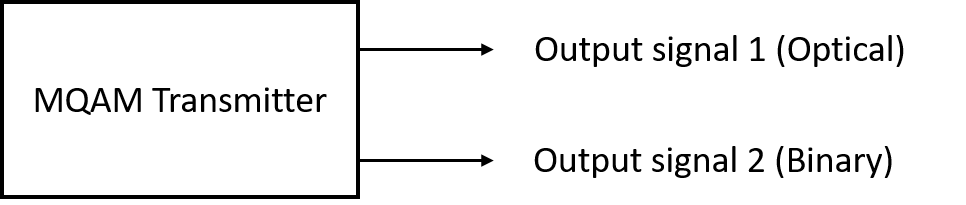
\includegraphics[width=0.5\textwidth]{figures/MQAM_transmitter_block_diagram_simple}
	\caption{Basic configuration of the MQAM transmitter}\label{MQAM_transmitter_block_diagram_simple}
\end{figure}

\subsection*{Functional description}

This block generates an optical signal (output signal 1 in figure \ref{MQAM_transmitter_block_diagram}). The binary signal generated in the internal block Binary Source (block B1 in figure \ref{MQAM_transmitter_block_diagram}) can be used to perform a Bit Error Rate (BER) measurement and in that sense it works as an extra output signal (output signal 2 in figure \ref{MQAM_transmitter_block_diagram}).

\begin{figure}[h]
	\centering
	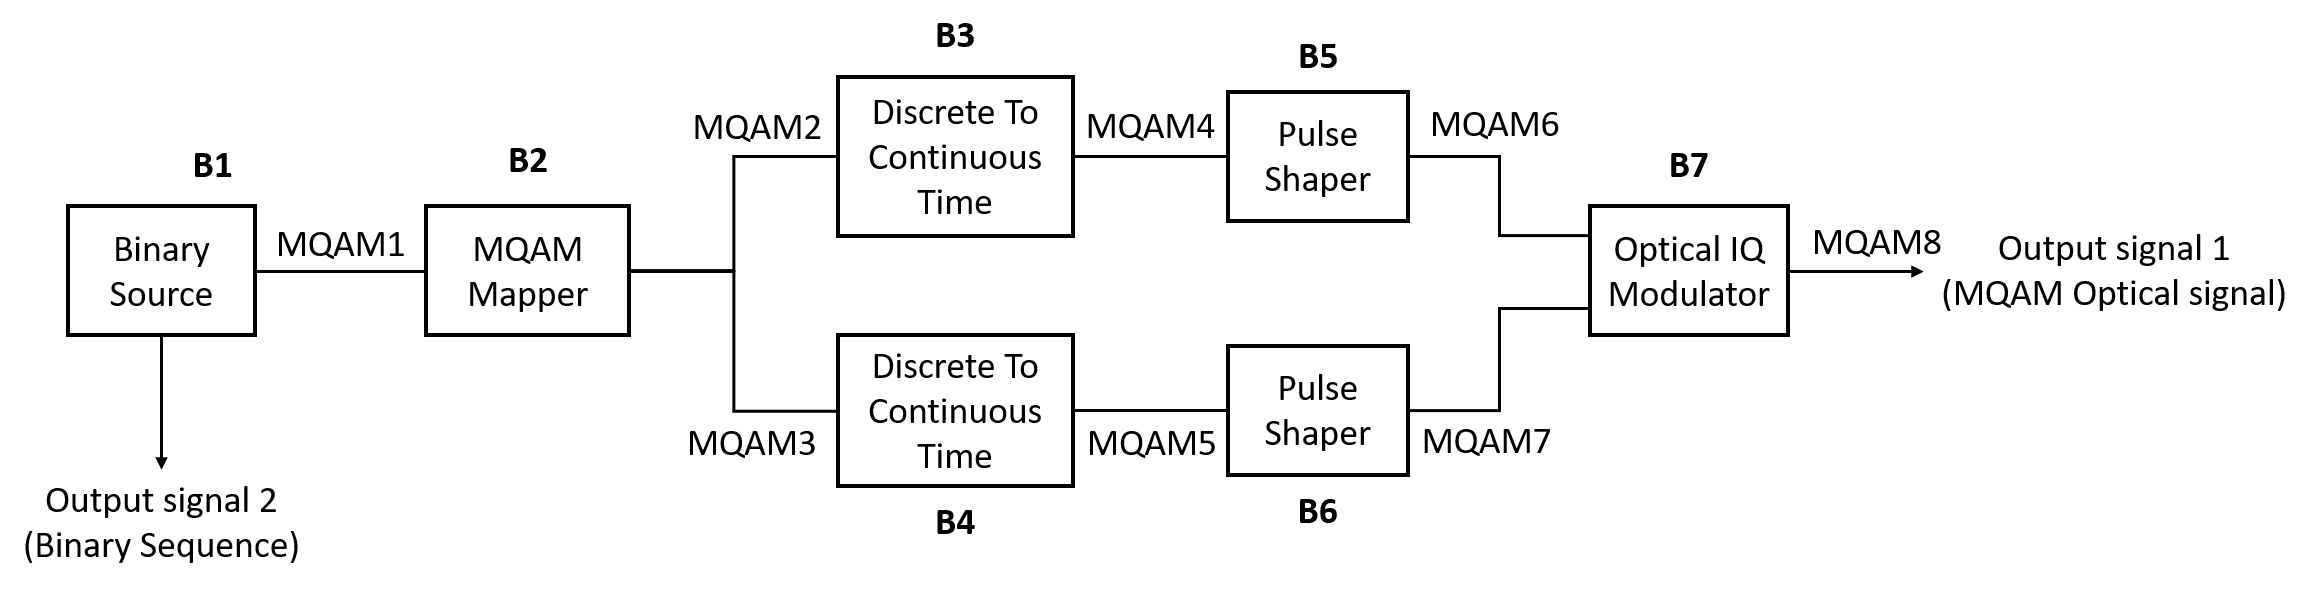
\includegraphics[width=\textwidth]{figures/MQAM_transmitter_block_diagram}
	\caption{Schematic representation of the block MQAM transmitter.}\label{MQAM_transmitter_block_diagram}
\end{figure}

\subsection*{Input parameters}

This block has a special set of functions that allow the user to change the basic configuration of the transmitter. The list of input parameters, functions used to change them and the values that each one can take are summarized in table \ref{table}.

\begin{table}[h]
\begin{center}
	\begin{tabular}{| m{3,5cm} | m{5,1cm} |  m{2,5cm} | m{4cm} | }
		\hline
		\textbf{Input parameters} & \textbf{Function} & Type & \textbf{Accepted values} \\ \hline
		Mode & setMode() & string & PseudoRandom \newline Random \newline DeterministicAppendZeros \newline DeterministicCyclic \\ \hline
		Number of bits generated & setNumberOfBits() & int & Any integer\\ \hline
		Pattern length & setPatternLength() & int & Real number greater than zero\\ \hline
		Number of bits & setNumberOfBits() & long & Integer number greater than zero\\ \hline
		Number of samples per symbol & setNumberOfSamplesPerSymbol() & int & Integer number of the type $2^n$ with n also integer\\ \hline
		Roll of factor & setRollOfFactor() & double & $\in$ [0,1] \\ \hline
		IQ amplitudes & setIqAmplitudes() & Vector of coordinate points in the I-Q plane & \textbf{Example} for a 4-qam mapping: \{ \{ 1.0, 1.0 \}, \{ -1.0, 1.0 \}, \{ -1.0, -1.0 \}, \{ 1.0, -1.0 \} \} \\ \hline
		Output optical power & setOutputOpticalPower() & int & Real number greater than zero\\ \hline
		Save internal signals & setSaveInternalSignals() & bool & True or False\\
		\hline
	\end{tabular}
	\caption{List of input parameters of the block MQAM transmitter} \label{table}
\end{center}
\end{table}

%\begin{itemize}
%	\item setMode(PseudoRandom);
%	\item setBitPeriod(1.0/50e9);
%	\linebreak (double)
%	\item setPatternLength(3);
%	\linebreak (int)
%	\item setNumberOfBits(10000);
%	\linebreak (long)
%	\item setNumberOfSamplesPerSymbol(32);
%	\linebreak (int)
%	\item setRollOffFactor(0.9);
%	\linebreak (double $\in$ [0,1])
%	\item setIqAmplitudes(\{ \{ 1, 1 \}, \{ -1, 1 \}, \{ -1, -1 \}, \{ 1, -1 \} \});
%	\item setOutputOpticalPower\_dBm(0);
%	\item setSaveInternalSignals(true);
%\end{itemize}

\pagebreak

\subsection*{Methods}

MQamTransmitter(vector$<$Signal *$>$ \&inputSignal, vector$<$Signal *$>$ \&outputSignal); (\textbf{constructor})
\bigbreak

void set(int opt);
\bigbreak
void setMode(BinarySourceMode m)
\bigbreak
BinarySourceMode const getMode(void)
\bigbreak
void setProbabilityOfZero(double pZero)
\bigbreak
double const getProbabilityOfZero(void)
\bigbreak
void setBitStream(string bStream)
\bigbreak
string const getBitStream(void)
\bigbreak
void setNumberOfBits(long int nOfBits)
\bigbreak
long int const getNumberOfBits(void)
\bigbreak
void setPatternLength(int pLength)
\bigbreak
int const getPatternLength(void)
\bigbreak
void setBitPeriod(double bPeriod)
\bigbreak
double const getBitPeriod(void)
\bigbreak
void setM(int mValue)
int const getM(void)
\bigbreak
void setIqAmplitudes(vector$<$t\textunderscore iqValues$>$ iqAmplitudesValues)
\bigbreak
vector$<$t\textunderscore iqValues$>$ const getIqAmplitudes(void)
\bigbreak
void setNumberOfSamplesPerSymbol(int n)
\bigbreak
int const getNumberOfSamplesPerSymbol(void)
\bigbreak
void setRollOffFactor(double rOffFactor)
\bigbreak
double const getRollOffFactor(void)
\bigbreak
void setSeeBeginningOfImpulseResponse(bool sBeginningOfImpulseResponse)
\bigbreak
double const getSeeBeginningOfImpulseResponse(void)
\bigbreak
void setOutputOpticalPower(t\textunderscore real outOpticalPower)
\bigbreak
t\textunderscore real const getOutputOpticalPower(void)
\bigbreak
void setOutputOpticalPower\_dBm(t\_real outOpticalPower\_dBm)
\bigbreak
t\_real const getOutputOpticalPower\_dBm(void)
\pagebreak

\subsection*{Output Signals}

\subparagraph*{Number:} 1 optical and 1 binary (optional)

\subparagraph*{Type:} Optical signal

\subsection*{Example}

\begin{figure}[h]
	\centering
	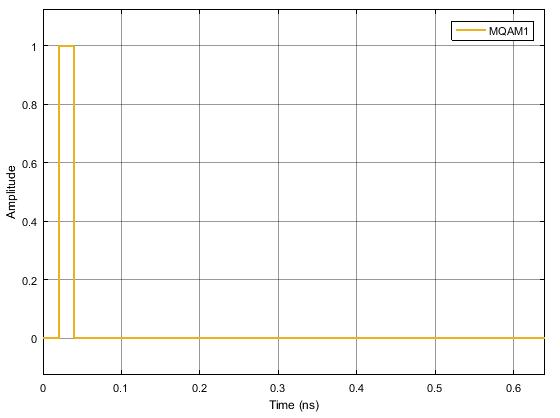
\includegraphics[width=0.8\textwidth]{figures/BinarySource_output}
	\caption{Example of the binary sequence generated by this block for a sequence 0100...}
\end{figure}

\begin{figure}[h]
	\centering
	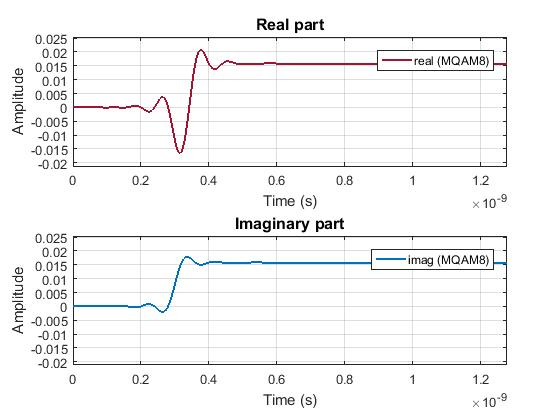
\includegraphics[width=0.8\textwidth]{figures/IQmodulator0_output}
	\caption{Example of the output optical signal generated by this block for a sequence 0100...}
\end{figure}

\subsection*{Sugestions for future improvement}

Add to the system another block similar to this one in order to generate two optical signals with perpendicular polarizations. This would allow to combine the two optical signals and generate an optical signal with any type of polarization.
 \fi
\ifdefined\optical      

\clearpage
\section{Optical Detection}

\begin{tcolorbox}	
\begin{tabular}{p{2.75cm} p{0.2cm} p{10.5cm}}
\textbf{Contributors}  &:& Nelson Muga, (2017-12-21 - ...)\\
                       &:& Diamantino Silva, (2017-08-18 - 2018-02-05)\\
                       &:& Armando Pinto (2017-08-15 - ...)\\
\textbf{Goal}          &:& Analise of various optical detection schemes.\\
\end{tabular}
\end{tcolorbox}
%
\vspace{2em}
%
The detection of light is a fundamental stage in every optical communication system, bridging the optical domain into the electrical domain.
This section will review various theoretical, practical, and implementation aspects of the most important light detection schemes.
The objective of this work is to develop numerical models for the various optical detections schemes and to validate such numerical models with experimental results.\\
%
%
\subsection{Theoretical Analysis} \label{subsec:intro}

\begin{tcolorbox}	
\begin{tabular}{p{2.75cm} p{0.2cm} p{10.5cm}}
\textbf{Contributors}  &:& Nelson Muga (2017-12-20 - )\\
                       &:& Diamantino Silva (2017-08-18 - ...)\\
                       &:& Armando Pinto (2017-08-15 - ...)\\
\textbf{Goal}          &:& Theoretical description of various optical detection schemes.\\
\end{tabular}
\end{tcolorbox}

In this subsection, we are going to calculate the signal-to-noise ratio at the input of the decision circuit for the various detection schemes under analysis.
For each detection scheme a classical and a quantum description is going to be developed and a comparative analysis is going to performed.

\subsubsection{Classical Description}

\begin{tcolorbox}	
\begin{tabular}{p{2.75cm} p{0.2cm} p{10.5cm}}
\textbf{Contributors}  &:& Nelson Muga (2017-12-20 - )\\
                       &:& Diamantino Silva (2017-08-18 - ...)\\
                       &:& Armando Pinto (2017-08-15 - ...)\\
\textbf{Goal}          &:& Develop a classical description of various optical detection schemes.\\
\end{tabular}
\end{tcolorbox}

{\bf \em Direct Detection}\\

One of the most simple detection methods is the direct detection of light with a single detector and the analysis of the resulting photocurrent.

\begin{figure}[H]
	\label{fig:detection_direct}
	\centering
	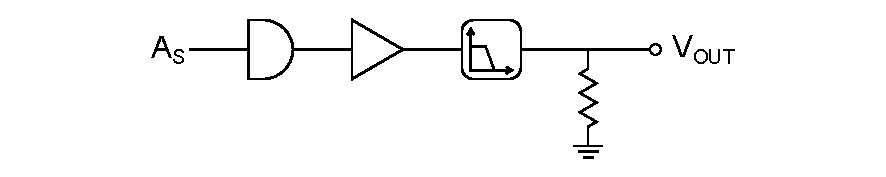
\includegraphics{./sdf/optical_detection/figures/detection-direct.pdf}
	\caption{Direct detection.}
\end{figure}

\noindent


Given an electric field generated by an ideal monochromatic single mode laser, it can be modulated in amplitude and phase by a signal $A(t)$ resulting in the function

\begin{equation}
    E_R(t)=\sqrt{2} |A(t)| cos\left(-\omega t + \theta\right) \,\,\,\, \sqrt{W}
\end{equation}
with $A(t)=|A(t)|e^{-i\theta(t)}$, and where $\omega_0$ is the carrier frequency and $\theta$ is the phase.

We will consider that the detector has a bandwidth $B$, greater that the signal $A(t)$, but much smaller than $2 \omega_0$. The calculation of power incident in the photodiode is given by the expected value of the square of the amplitude during a time interval $\Delta t = 2 \pi / \omega$\\

Measurable optical power, assuming that the detector bandwidth, $B$, is greater than the signal, $A(t)$, bandwidth but much small than $2 \omega_0$

\begin{align}
	P(t)	&= \overline{E_R^2(t)}\nonumber\\
			&= \overline{|A(t)|^2} + \overline{ |A(t)|^2 cos\left(-2 \omega t + 2\theta(t)\right)}\nonumber\\
         &= |A(t)|^2 \,\,\,\, W
\end{align}


\vspace{2em}
\noindent
To simplify calculations, the electric field can be expressed the complex notation
%
\begin{equation}
	E(t) = A(t) e^{-i \omega_0 t}
\end{equation}
%
%
The physically measurable quantities are obtained by taking the real part of the complex wave. Using this notation, the beam power, $P(t)$, is obtained by multiplying the electric field's conjugate by itself

\begin{align}
	P(t) &= E^{*}(t) E(t)\nonumber\\
         &= |A(t)|^2
\end{align}

\begin{equation}
	i(t) = \eta q \frac{P(t)}{\hbar \omega_0}
\end{equation}
in which $\eta$ is the photodiode's responsivity, q is the unit charge and $P(t)/\hbar \omega_0$ is the number of removed electrons.

The signal is ...
\begin{equation}
	E(t) = A(t) e^{-i \omega_0}
\end{equation}
Using the definition of electric power of a complex electric field representation, we will get
\begin{equation}
	P(t) = |A(t)|^2
	\label{eq:power}
\end{equation}
recovering the result of the real representation. The photocurrent can be rewriten as a function of the signal $A(t)$

\begin{equation}
	i(t) = \eta q \frac{|A(t)|^2}{\hbar \omega_0}
\end{equation}
which will use to express the second moment of the photocurrent as
\begin{equation}
	\langle i^2(t) \rangle = \eta^2 q^2 \frac{\langle |A(t)|^4 \rangle }{\hbar^2 \omega_0^2}
\end{equation}
Assuming a fase modulation, in which the amplitude is constant, the signal is simplified to
\begin{equation}
	A(t) = |A| e^{i \theta}
\end{equation}
Therefore, the current becomes constant
\begin{equation}
	i(t) = I_0 = \eta q \frac{A_s^2}{\hbar \omega_0}
\end{equation}
and it's second moment becomes simply
\begin{equation}
	\langle i^2(t) \rangle = I_0^2
\end{equation}

Shot noise in photodiodes\\

\begin{equation}
	\langle i_n^2(t) \rangle = 2 q B I_0
\end{equation}

The signal to noise ratio is obtained by the relation between the second moment of the sinal to the second moment of the noise

\begin{align}
	\frac{S}{N} &= \frac{\langle i^2(t) \rangle}{\langle i_n^2(t) \rangle} \nonumber\\
                &= \frac{I_0}{2 q B}\nonumber\\
                &= \eta \frac{ |A|^2}{\hbar \omega_0 B}
\end{align}

{\bf \em Homodyne Detection}\\

\begin{figure}[H]
	\centering
	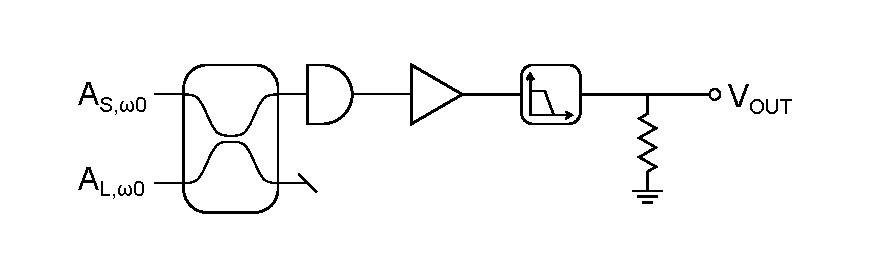
\includegraphics{./sdf/optical_detection/figures/detection-homodyne.pdf}
	\caption{Homodyne detection.}
\end{figure}
%%
The homodyne detection scheme uses an auxiliary local oscillator, which is combined in
a beamsplitter with the signal beam. After this step, it is similar to the direct detection. As we will see this has some implications in the phase detection???\\
\\
Given a splitter with intensity transmission $\epsilon$, the resulting field incident to the photodetector is
\cite{shapiro1985quantum} %p.241
%
\begin{equation}
	E(t) = \sqrt{\epsilon}E_S(t) + \sqrt{1-\epsilon}E_{LO}(t)
\end{equation}
%
in which $E_{LO} = e^{i \omega_0 t}$.
Given a local oscillator with a much larger power that the signal, then, the incident power in the photodiode is
%
\begin{align}
	P(t)	&= \eta \left[ (1-\epsilon) P_{LO}(t) + 2 \sqrt{\epsilon (1-\epsilon)} \textrm{Re} \left[ E_S(t) E^\ast_{LO}(t) \right] \right]\\
			&= \eta \left[ (1-\epsilon) P_{LO}(t) + 2 \sqrt{\epsilon (1-\epsilon)} |E_S(t)| |E_{LO}(t)| \cos{(\phi)} \right]\\
\end{align}

{\bf \em Balanced Homodyne Detection}\\
%
%

\begin{figure}[H]
	\centering
	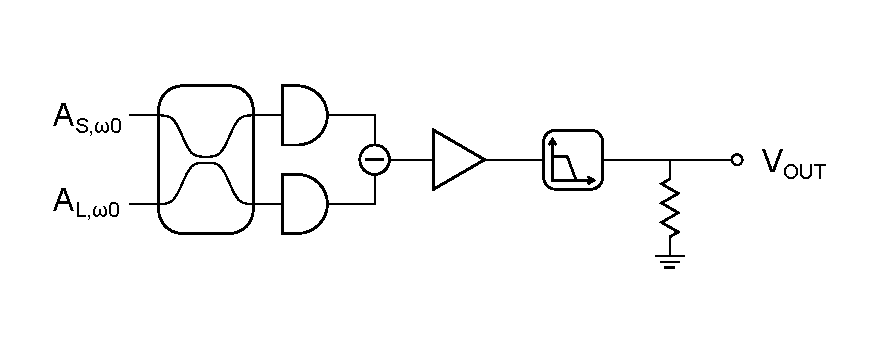
\includegraphics{./sdf/optical_detection/figures/detection-balanced-homodyne.pdf}
	\caption{Balanced homodyne detection.}
\end{figure}
%%
"In a balanced homodyne detector (BHD), the signal to be measured is mixed with a local oscillator (LO) at a beam splitter. The interference signals from the two output ports of the beam splitter are sent to two photodiodes followed by a subtraction operation, and then, amplification may be applied. The output of a BHD can be made to be proportional to either the amplitude quadrature or the phase quadrature of the input signal depending on the relative phase between the signal and the LO".
\\
\\
\\
{\bf \em IQ Homodyne Balanced Detection}\\

%%
\begin{figure}[H]
	\centering
	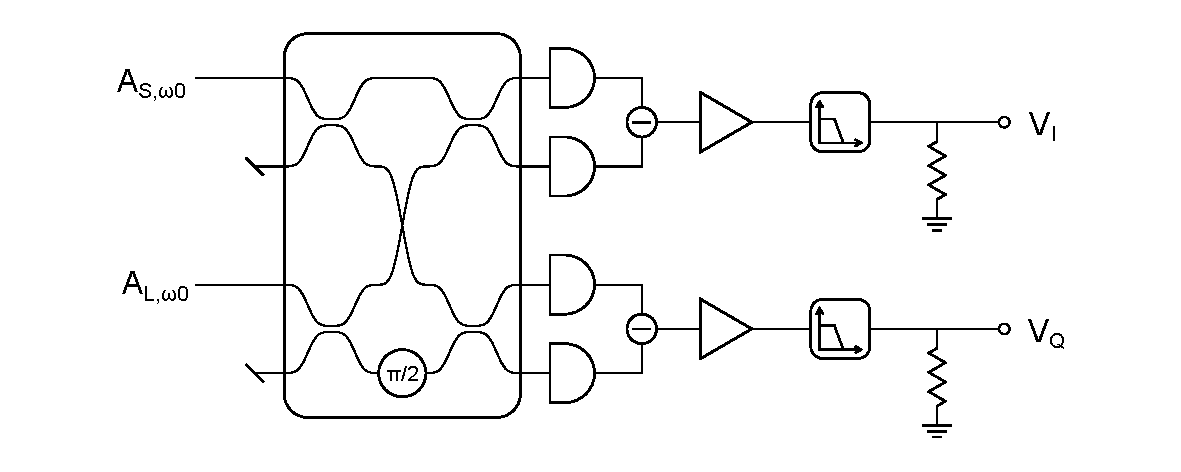
\includegraphics[width=15cm]{./sdf/optical_detection/figures/detection-IQ-balanced-homodyne.pdf}
	\caption{IQ balanced homodyne detection.}
\end{figure}
\noindent
{\bf \em Semiclassical model}\\
\\
{\bf \em Quantum model}\\


\begin{figure}[H]
	\centering
	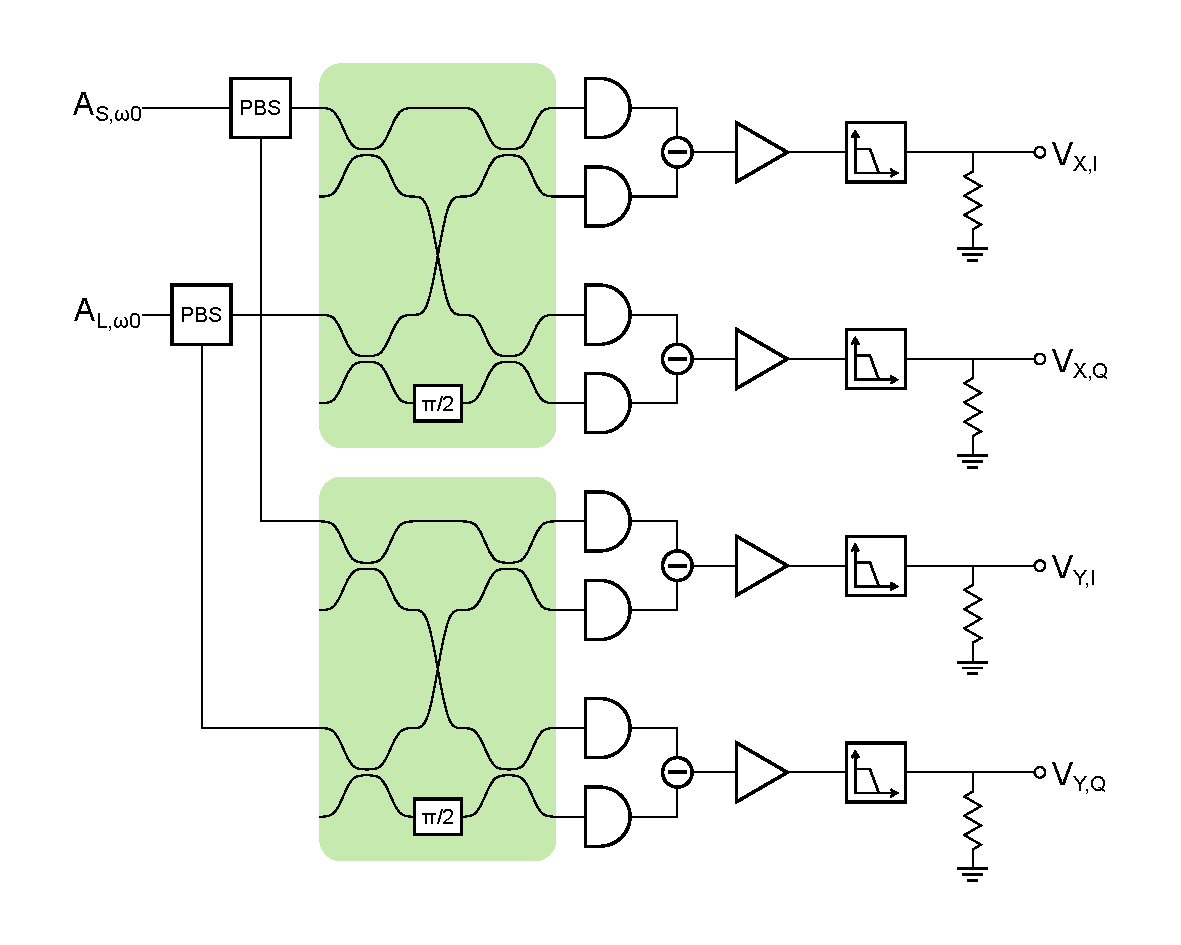
\includegraphics[width=15cm]{./sdf/optical_detection/figures/detection-double-polarized-IQ-balanced-homodyne.pdf}
	\caption{Double polarized IQ balanced homodyne detection.}
\end{figure}


\paragraph{Heterodyne Detection}\ \\
%%
\begin{figure}[H]
	\centering
	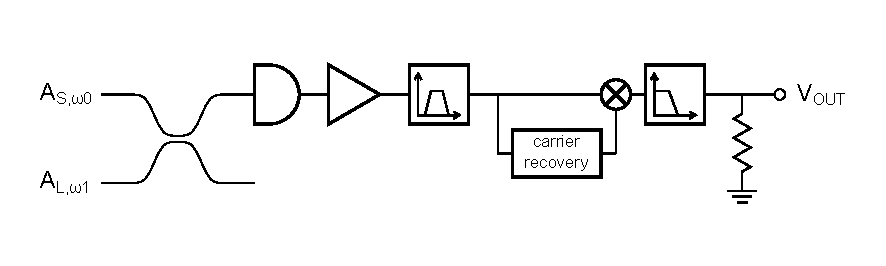
\includegraphics{./sdf/optical_detection/figures/detection-heterodyne.pdf}
	\caption{Heterodyne detection.}
\end{figure}

% inventado
In contrast with the homodyne detection, in which the frequency of the signal carrier is equal to the frequency of the local oscillator, in the heterodyne detection, these frequencies are different.\\
Because of this, the inference will result in a new signal with an intermediate frequency at...\\
% PROCURAR REFERENCIAS
\\



\paragraph{Balanced Heterodyne Detection}\ \\
%%
\begin{figure}[H]
	\centering
	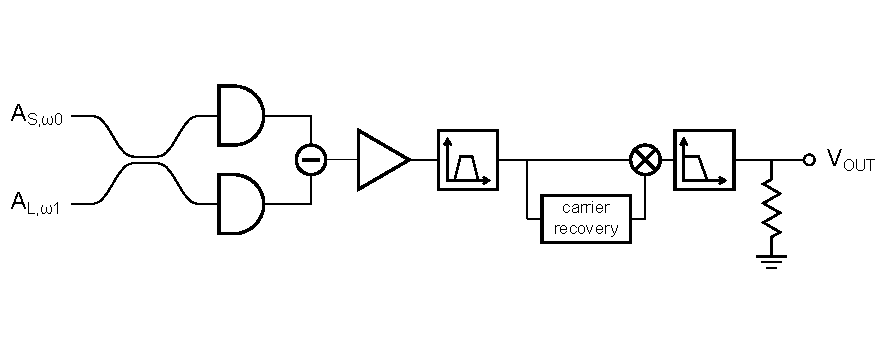
\includegraphics{./sdf/optical_detection/figures/detection-balanced-heterodyne.pdf}
	\caption{Balanced heterodyne detection.}
\end{figure}
%
\noindent
{\bf \em Semiclassical model}\\
\\
{\bf \em Quantum model}\\


\paragraph{IQ Heterodyne Balanced Detection}\ \\
%
\begin{figure}[H]
	\centering
	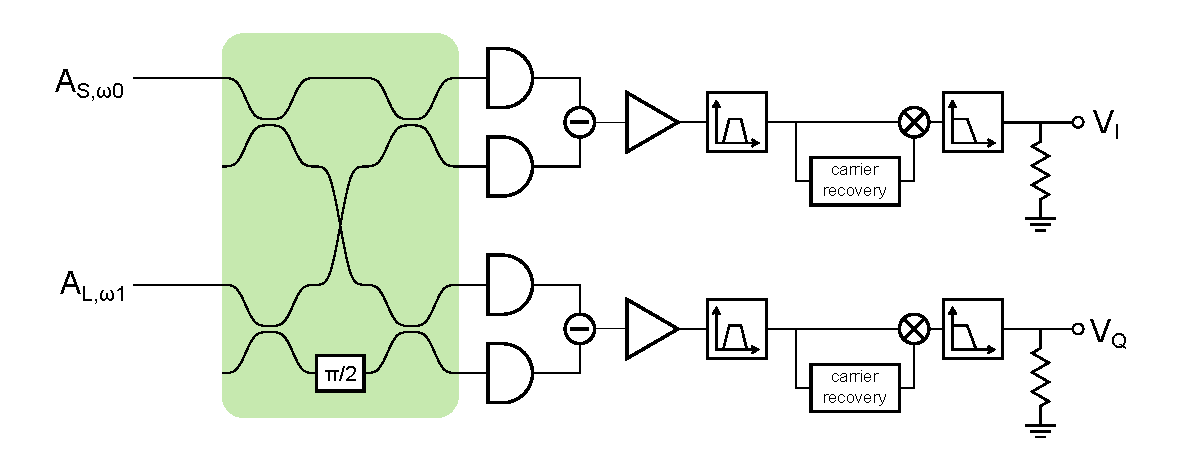
\includegraphics[width=15cm]{./sdf/optical_detection/figures/detection-IQ-balanced-heterodyne.pdf}
	\caption{IQ balanced heterodyne detection.}
\end{figure}


\begin{figure}[H]
	\centering
	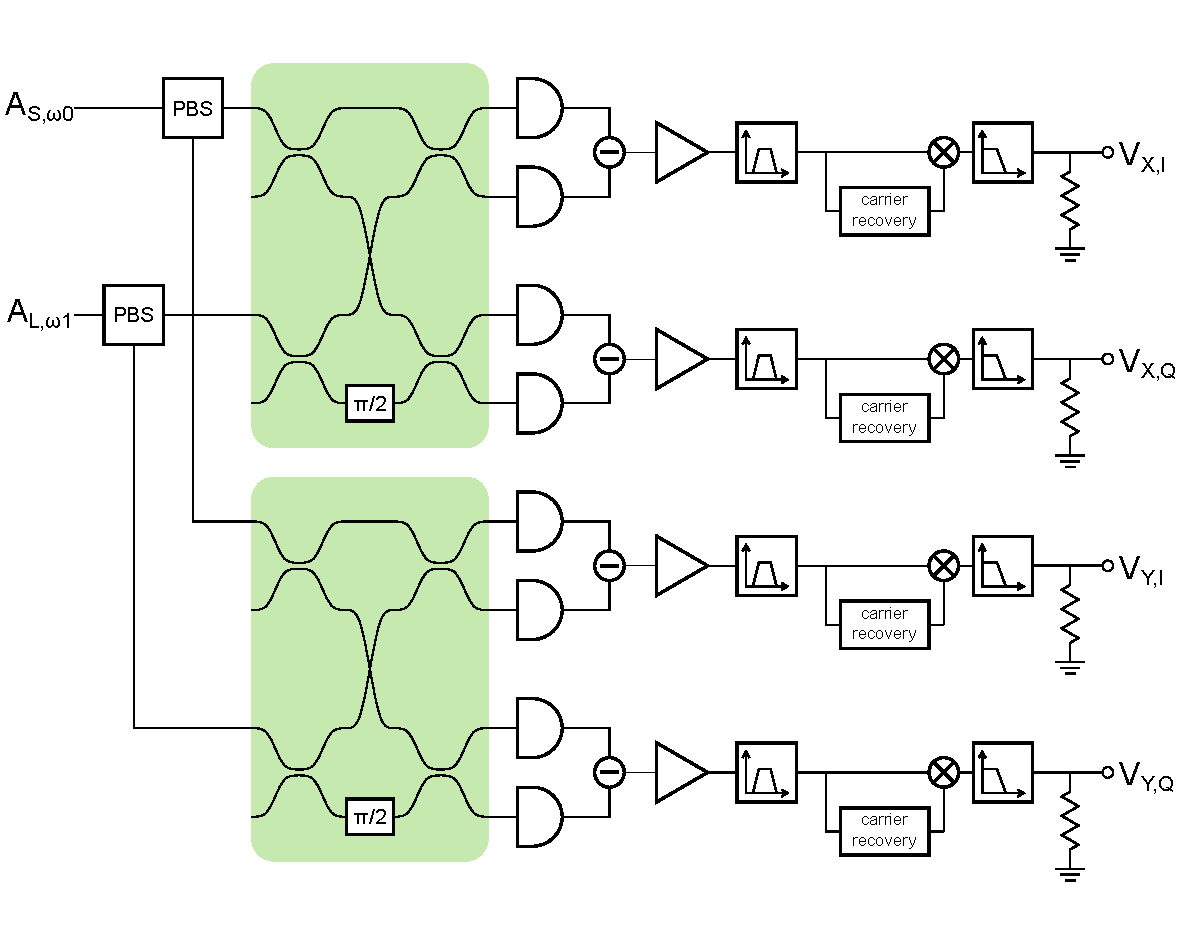
\includegraphics[width=15cm]{./sdf/optical_detection/figures/detection-double-polarized-IQ-balanced-heterodyne.pdf}
	\caption{Double polarized IQ balanced heterodyne detection.}
\end{figure}


%
\noindent
\subsubsection{Thermal noise}
Thermal noise is generated by electrons in response to temperature. It's contribution to the resulting current can be described by the following equation
\cite{fox2006}
%\footnote{Mark Fox, p. 96}
%
\begin{equation}
\braket{(\Delta i_T)^2} = 4 K_B T_0 B/R_L
\end{equation}
%
in which $K_B$ it's Boltzmann's constant, $T_0$ is the absolute temperature, $B$ is the bandwidth and $R_L$ is the receiver load impedance. The $B$ value is imposed by default or chosen when the measurements are made, but the $R_L$ value is dependent in the internal setup of the various components of the detection system. Nevertheless, for simulation purposes, we can just introduce an experimental value.\\
\vspace{1cm}
%
%


\subsubsection{Quantum Description}

\begin{tcolorbox}	
\begin{tabular}{p{2.75cm} p{0.2cm} p{10.5cm}}
\textbf{Contributors}  &:& Diamantino Silva (2017-08-18 - ...)\\
                       &:& Armando Pinto (2017-08-15 - ...)\\
\textbf{Goal}          &:& Develop a quantum description of various optical detection schemes, and compare with the classical description.\\
\end{tabular}
\end{tcolorbox}

We start by defining number states $\ket{n}$ (or Fock states), which correspond to states with perfectly fixed number of photons
%\footnote{Loundon, p.184}
\cite{loudon2000}.
Associated to those states are two operators, the creation $\hat{a}^\dagger$ and annihilation $\hat{a}$ operators, which in a simple way, remove or add one photon from a given number state
%\footnote{Mark Fox, p.155}
\cite{fox2006}.
Their action is defined as
%
\begin{center}
	\hspace{-4mm}
	\begin{minipage}{44mm}
		\noindent
		\begin{equation}
			\hat{a} \ket{n} = \sqrt{n} \ket{n-1}
		\end{equation}
	\end{minipage}
	$,\quad$
	\begin{minipage}{52mm}
		\noindent
		\begin{equation}
			\hat{a}^\dagger \ket{n} = \sqrt{n+1} \ket{n+1}
		\end{equation}
	\end{minipage}
	$,\quad$
	\begin{minipage}{35mm}
		\noindent
		\begin{equation}
			\hat{n} \ket{n} = n \ket{n}
		\end{equation}
	\end{minipage}
\end{center}
%
in which $\hat{n} = \hat{a}^\dagger\hat{a}$ is the number operator. Therefore, number states are eigenvectors of the number operator.\\
\\
Coherent states have properties that closely resemble classical electromagnetic waves, and are generated by single-mode lasers well above the threshold.
\cite{loudon2000}
%\footnote{Loudon, p.190}
We can defined them, using number states in the following manner
\begin{equation}
\ket{\alpha} = e^{-\frac{|\alpha|^2}{2}} \sum_{n=0}^\infty \frac{\alpha^n}{\sqrt{n!}} \ket{n}
\end{equation}
in which the complex number $\alpha$ is the sole parameter that characterizes it.
%\footnote{Loudon, p.184}
%\footnote{Loudon, p.186}
In fact, if we calculate the expected number of photons with $\bra{\alpha} \hat{n} \ket{\alpha}$ we will obtain $|\alpha|^2$. The coherent state is an eigenstate of the annihilation operator, $\hat{a}\ket{\alpha} = \alpha \ket{\alpha}$.\\
\\
%
%
Using the creation and annihilation operators, we can define two quadrature operators
\cite{loudon2000}
%\footnote{Loudon, p.138, (4.3.36)}
%
\begin{center}
	\begin{minipage}{41mm}
		\noindent
		\begin{equation}
			\hat{X} = \frac{1}{2} \left( \hat{a}^\dagger + \hat{a} \right)
		\end{equation}
	\end{minipage}
	$,\quad$
	\begin{minipage}{40mm}
		\noindent
		\begin{equation}
			\hat{Y} = \frac{i}{2} \left( \hat{a}^\dagger - \hat{a} \right)
		\end{equation}
	\end{minipage}
\end{center}
%
The expected value of these two operators, using a coherent state $\ket{\alpha}$ are
%
\begin{center}
	\begin{minipage}{37mm}
		\noindent
		\begin{equation}
			\braket{\hat{X}} = \textrm{Re}(\alpha)
		\end{equation}
	\end{minipage}
	$,\quad$
	\begin{minipage}{37mm}
		\noindent
		\begin{equation}
			\braket{\hat{Y}} = \textrm{Im}(\alpha)
		\end{equation}
	\end{minipage}
\end{center}
%
We see that the expected value of these operators give us the real and imaginary part of $\alpha$. Now, we can obtain the uncertainty of these operators, using:
%
\begin{equation}
\textrm{Var}(\hat{X}) = \braket{\hat{X}^2} - \braket{\hat{X}}^2
\end{equation}
%
For each of these quadrature operators the variance will be
%
\begin{equation}
\textrm{Var}(\hat{X}) = \textrm{Var}(\hat{Y}) = \frac{1}{4}
\end{equation}
%
This result show us that for both quadratures, the variance of measurement is the same and independent of the value of $\alpha$.
%
%
%
\subsubsection{Homodyne detection}

The measurent of a quadrature of an input signal (S) is made by using the balanced homodyne detection technique, which measures the phase difference between the input signal and a local oscillator (LO). The measurement of quadrature are made relative to a reference phase of the LO, such that if the measurement is made in-phase with this reference, the value will be proportional to the $\hat{X}$ quadrature of the signal. If the phase of the LO is has an offset of $\pi/2$ relative to the reference, the output will be proportional to the $\hat{Y}$ quadrature of the signal.\\
\\
Experimentally, the balanced homodyne detection requires a local oscillator with the same frequency as the input signal, but with a much larger amplitude. These two signals are combined using a 50:50 beam splitter, from were two beams emerge, which are then converted to currents using photodides. Finally, the two currents are subtracted, resulting in an output current proportional to a quadrature of the input signal
\cite{fox2006}.\\
%\footnote{Mark Fox, p. 140}
%
%The balanced homododyne technique is used to measure the phase of the input signal (S), relative to the phase of a local oscillator (LO), which has the same frequency as the input signal, but a much larger amplitude. The technique consists in combining the input signal and the local oscillator, using a 50:50 beam splitter, from whom two beams emerge, which are then converted to currents using photodides. Finally, the two currents are subtracted, resulting in an output current.\\
A phase of the local oscillator can be defined as the reference phase. A phase offset equal to $0$ or $\pi/2$ will give an output proportional to the signal's in-phase component or to the quadrature component, respectively. Therefore, the $\hat{X}$ operator will correspond to the in-phase component and $\hat{Y}$ operator correspond to quadrature component
%\cite{fox2006}.
%\footnote{Mark Fox, p. 140}
\\
%
\begin{figure}[H]
	\label{fig:scheme_homodyne}
	\centering
	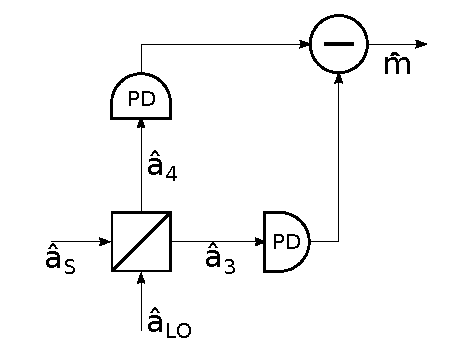
\includegraphics{./sdf/optical_detection/figures/scheme_homodyne.pdf}
	\caption{Balanced homodyne detection.}
\end{figure}
%
In the lab and in our simulations, a more complex system is used, the double balanced homodyne detection, which allows the simultaneous measurement of the $\hat{X}$ and $\hat{Y}$ components. The signal is divided in two beam with half the power of the original. One of the beams is used in a balanced homodyne detection with a local oscillator. The other beam is used in another balanced homodyne detection, but using a local oscillator with a phase difference $\pi/2$ relative to the first one.
%
\begin{figure}[H]
	\label{fig:scheme_homodyne}
	\centering
	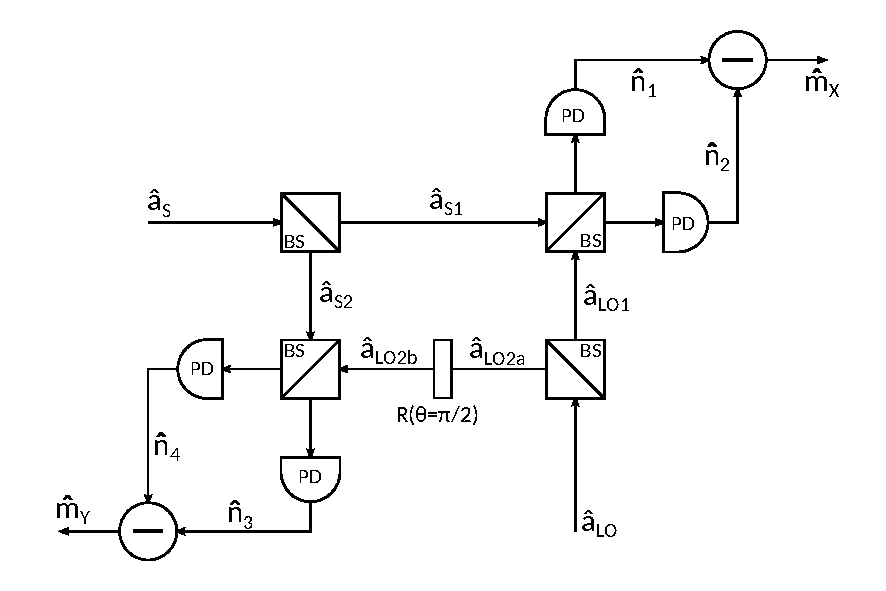
\includegraphics{./sdf/optical_detection/figures/scheme_double_homodyne.pdf}
	\caption{Balanced double homodyne detection.}
\end{figure}
%
%
%
\subsubsection{Noise sources in homodyne detection}
The detection of light using photodiodes is subjected to various sources of noise. One of these sources is the electrical field itself. The interaction of the signal with the vaccuum field adds quantum noise to the detection.
Another source of noise comes from the detection system, such as photodiodes and other electrical circuits, originating various kinds of noise, such as thermal noise, dark noise and amplifier noise
%\footnote{Hans, p.185}
\cite{hans2004}.
In the following sections, we will focus on two noise sources, quantum noise and thermal noise.
%
%
%
\subsubsection{Quantum Noise}
In order to grasp this effect, the quantum mechanical description of balanced homodyne detection will be used, employing quantum operators to describe the effect of each component in the system (fig. \ref{fig:scheme_homodyne}). We start with the operators $\hat{a}_S$ and $\hat{a}_{LO}$ corresponding to the annihilation operator for the signal and local oscillator, which are the inputs in a beam divisor. The outputs will be $\hat{a}_3$ and $\hat{a}_4$.
Using a balanced beam splitter, we can write the output as
%
\begin{center}
	\begin{minipage}{48mm}
		\noindent
		\begin{equation}
			\hat{a}_3 = \frac{1}{\sqrt{2}} \left( \hat{a}_S + \hat{a}_{LO} \right)
		\end{equation}
	\end{minipage}
	$,\quad$
	\begin{minipage}{48mm}
		\noindent
		\begin{equation}
			\hat{a}_4 = \frac{1}{\sqrt{2}} \left( \hat{a}_S - \hat{a}_{LO} \right)
		\end{equation}
	\end{minipage}
\end{center}
%
The final output of a homodyne measurement will be proportional to the difference between the photocurrents in arm $3$ and $4$. Then
%
\begin{equation}
I_{34} = I_3 - I_4 \sim \braket{\hat{n}_3 - \hat{n}_4}
\end{equation}
%
We can define an operator that describes the difference of number of photons in arm 3 and arm 4:
%
\begin{equation}
\hat{m} = \hat{a}^\dagger_3\hat{a}_3 - \hat{a}^\dagger_4\hat{a}_4
\end{equation}
%
If we assume that the local oscillator produces the the coherent state $\ket{\beta}$, then the expected value of this measurement will be
%
\begin{center}
	\begin{minipage}{58mm}
		\noindent
		\begin{equation}
			\braket{m} = 2|\alpha||\beta|\cos({\theta_\alpha - \theta_\beta})
		\end{equation}
	\end{minipage}
	$,\quad$
	\begin{minipage}{46mm}
		\noindent
		\begin{equation}
			\textrm{Var}(m) = |\alpha|^2 + |\beta|^2
		\end{equation}
	\end{minipage}
\end{center}
%
The local oscillator normally has a greater power than the signal
%VER REFERENCIAS
, then $|\alpha| \ll |\beta|$. If we use as unit, $2|\beta|$, then these two quantities can be simplified to
%
\begin{center}
	\begin{minipage}{52mm}
		\noindent
		\begin{equation}
			\label{eq:var_m}
			\braket{m} = |\alpha|\cos({\theta_\alpha - \theta_\beta})
		\end{equation}
	\end{minipage}
	$,\quad$
	\begin{minipage}{34mm}
		\noindent
		\begin{equation}
			\textrm{Var}(m) \approx \frac{1}{4}
		\end{equation}
	\end{minipage}
\end{center}
%
\cite{hans2004}
%\footnote{Referencia indirecta: Livro: Hans, p.207}
\\
Has we have seen previously, in order to measure two quadratures simultaneously, we can use double balanced homodyne detection. For each quadrature, the input signal now has half the power, so $|\alpha| \rightarrow |\alpha/\sqrt{2}|$.  If we use a local oscillator that produces states $\ket{\beta}$, then we can divide it in two beams in state $\ket{\beta/\sqrt{2}}$ and $\ket{i\beta/\sqrt{2}}$ which will be used in each homodyne detection. In this setting, the expected values for each quadrature, $X$ and $Y$, (in normalized values of $\sqrt{2}|\beta|$) are
%
\begin{center}
	\begin{minipage}{58mm}
		\noindent
		\begin{equation}
			\braket{m_X} = \left|\frac{\alpha}{\sqrt{2}}\right| \cos({\theta_\alpha - \theta_\beta})
		\end{equation}
	\end{minipage}
	$,\quad$
	\begin{minipage}{37mm}
		\noindent
		\begin{equation}
			\textrm{Var}(m_X) \approx \frac{1}{4}
		\end{equation}
	\end{minipage}
\end{center}
%
%
\begin{center}
	\begin{minipage}{58mm}
		\noindent
		\begin{equation}
			\braket{m_Y} =  \left|\frac{\alpha}{\sqrt{2}}\right| \sin({\theta_\alpha - \theta_\beta})
		\end{equation}
	\end{minipage}
	$,\quad$
	\begin{minipage}{37mm}
		\noindent
		\begin{equation}
			\textrm{Var}(m_Y) \approx \frac{1}{4}
		\end{equation}
	\end{minipage}
\end{center}
%
Therefore the measurement of each quadrature will have half the amplitude, but the same variance.
%
%
% 

\subsection{Simulation Analysis}

\begin{tcolorbox}	
\begin{tabular}{p{2.75cm} p{0.2cm} p{10.5cm}}
\textbf{Contributors}  &:& Diamantino Silva, (2017-08-18 - ...)\\
\textbf{Goal}          &:& Simulation of various optical detection schemes.\\
\textbf{Directory}     &:& sdf/optical\_detection
\end{tabular}
\end{tcolorbox}
%
\vspace{2em}
%



\begin{figure}[H]
\centering
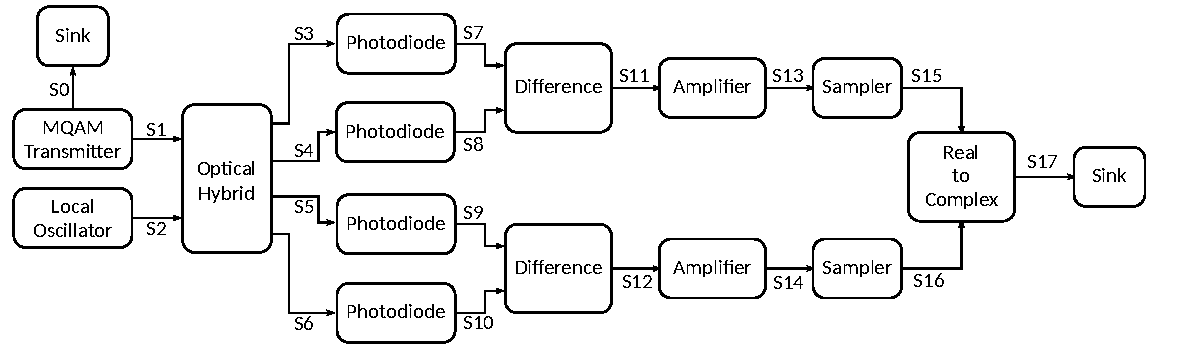
\includegraphics[width=\linewidth]{./sdf/optical_detection/figures/scheme_setup.pdf}
\caption{Overview of the simulated optical system.}
\label{fig:setup}
\end{figure}
%
\vspace{1em}
%
List of signals used in the simulation:
\begin{table}[H]
\centering
\begin{tabular}{|c|l|l|}
\hline
\bf{Signal name}	& \bf{Signal type}						& \bf{Status}\\
\hline
S0					& Binary								& check\\
S1					& OpticalSignal							& check\\
S2					& OpticalSignal							& check\\
S3					& OpticalSignal							& check\\
S4					& OpticalSignal							& check\\
S5					& OpticalSignal							& check\\
S6					& OpticalSignal							& check\\
S7					& TimeContinuousAmplitudeContinuousReal	& check\\
S8					& TimeContinuousAmplitudeContinuousReal	& check\\
S9					& TimeContinuousAmplitudeContinuousReal	& check\\
S10					& TimeContinuousAmplitudeContinuousReal	& check\\
S11					& TimeContinuousAmplitudeContinuousReal	& check\\
S12					& TimeContinuousAmplitudeContinuousReal	& check\\
S13					& TimeContinuousAmplitudeContinuousReal	& check\\
S14					& TimeContinuousAmplitudeContinuousReal	& check\\
S15					& TimeDiscreteAmplitudeContinuousReal	& check\\
S16					& TimeDiscreteAmplitudeContinuousReal	& check\\
S17					& OpticalSignal							& check\\
\hline
\end{tabular}
\end{table}
%
\vspace{2em}
%
This system takes into account the following input parameters:
\begin{table}[H]
\centering
\begin{tabulary}{1.0\textwidth}{|c|p{30mm}|p{70mm}|}
\hline
\textbf{System Parameters}	& {\bf Default value}		& \textbf{Description}\\
\hline
localOscillatorPower1		& $2.0505 \times 10^{-8}$W	& Sets the optical power, in units of W, of the local oscillator inside the MQAM\\
\hline
localOscillatorPower2		& $2.0505 \times 10^{-8}$W	& Sets the optical power, in units of W, of the local oscillator used for Bob's measurements\\
\hline
localOscillatorPhase		& $0$ rad					& Sets the initial phase of the local oscillator used in the detection\\
\hline
responsivity				& $1$ A/W					& Sets the responsivity of the photodiodes used in the homodyne detectors\\
\hline
iqAmplitudeValues			& $\{ \{ 1, 1 \}, \{ -1, 1 \},$ $ \{ -1, -1 \}, \{ 1, -1 \} \}$
														& Sets the amplitude of the states used in the MQAM\\
%
%\hline
%transferMatrix				&
%							$\frac{1}{\sqrt{2}}\{1,1,1,1\}$	
%							& Sets the transfer matrix of the beam splitter used in the homodyne detector\\
%\hline
%shotNoise (FUTURE)      & Chooses if quantum shot noise is used in the simulation\\
%\hline
%thermalNoise (FUTURE)   & Chooses if thermal noise is used in the simulation\\
%\hline
%thermalNoiseAmplitude  (FUTURE)  & Sets the amplitude of the thermal noise\\
%
\hline
\end{tabulary}
\end{table}
%
\vspace{2em}
%
The simulation setup is represented in figure \ref{fig:setup}. The starting point is the MQAM, which generates random states from the constelation given by the variable \texttt{iqAmplitudeValues}. The output from the generator is received in the Optical Hybrid where it is mixed with a local oscillator, outputing two optical signal pairs. Each pair is converted to currents by two photodiodes, and the same currents are subtracted from each other, originating another current proportional to one of the quadratures of the input state.
The other pair suffers the same process, but the resulting subtraction current will be proportional to another quadrature, dephased by $\pi/2$ relative to the other quadrature.\\
%
%\begin{table}[H]
%\centering
%\begin{tabular}{c|c}
%System Blocks                         & netxpto Blocks\\
%\hline
%M - Quadrature Amplitude Modulator    & MQamTransmitter\\
%Local Oscillator                      & LocalOscillator\\
%90deg Optical Hybrid                  & OpticalHybrid\\
%Photodiode                            & Photodiode\\
%Difference Circuit                    & Difference\\
%Sampler                               & Sampler\\
%\end{tabular}
%\end{table}


\subsection*{Required files}\label{Required files}

Header Files
\begin{table}[H]
\centering
\begin{tabulary}{1.0\textwidth}{|L|L|l|}
\hline
\textbf{File}			& \textbf{Description}									& {\bf Status}\\
\hline
netxpto.h               & Generic purpose simulator definitions.				& check\\
\hline
m\_qam\_transmitter.h   & Outputs a QPSK modulated optical signal.				& check\\
\hline
local\_oscillator.h     & Generates continuous coherent signal.					& check\\
\hline
optical\_hybrid.h       & Mixes the two input signals into four outputs.		& check\\
\hline
photodiode.h            & Converts an optical signal to a current.				& check\\
\hline
difference.h            & Ouputs the difference between two input signals.		& check\\
\hline
ideal\_amplifier.h		& Performs a perfect amplification of the input sinal	& check\\
\hline
sampler.h               & Samples the input signal.								& check\\
\hline
real\_to\_complex.h		& Combines two real input signals into a complex signal	& check\\
\hline
sink.h                  & Closes any unused signals.							& check\\
\hline
\end{tabulary}
\end{table}
%
%
Source Files
\begin{table}[H]
\centering
\begin{tabulary}{1.0\textwidth}{|L|L|l|}
\hline
\textbf{File}			& \textbf{Description}									& {\bf Status}\\
\hline
netxpto.cpp				& Generic purpose simulator definitions.				& check\\
\hline
m\_qam\_transmitter.cpp	& Outputs a QPSK modulated optical signal.				& check\\
\hline
local\_oscillator.cpp	& Generates continuous coherent signal.					& check\\
\hline
optical\_hybrid.cpp		& Mixes the two input signals into four outputs.		& check\\
\hline
photodiode.h			& Converts an optical signal to a current.				& check\\
\hline
difference.h			& Ouputs the difference between two input signals.		& check\\
\hline
ideal\_amplifier.h		& Performs a perfect amplification of the input sinal	& check\\
\hline
sampler.cpp				& Samples the input signal.								& check\\
\hline
real\_to\_complex.cpp	& Combines two real input signals into a complex signal	& check\\
\hline
sink.cpp				& Empties the signal buffer.							& check\\
\hline
\end{tabulary}
\end{table}



%\subsection*{Inputs}

%This system takes no inputs.

%\pagebreak
%\subsection*{Outputs}

%The system outputs the following objects:
%\begin{itemize}
%\item Signals:
%\begin{itemize}
%\item Binary Sequence used in the MQAM; (S$_{0}$)
%\item Local Oscillator used in the MQAM; (S$_{1}$)
%\item Local Oscillator used in the detection; (S$_{2}$)
%\item Optical Hybrid Outputs; (S$_{3}$, S$_{4}$, S$_{5}$, S$_{6}$)
%\item In phase Photodiodes output; (S$_{7}$, S$_{8}$)
%\item Quadrature Photodiode output; (S$_{9}$, S$_{10}$)
%\item In phase Difference output; (S$_{11}$)
%\item Quadrature Difference output; (S$_{12}$)
%\item In phase Sampler output; (S$_{13}$)
%\item Quadrature Sampler output; (S$_{14}$)
%\end{itemize}
%\end{itemize}


\pagebreak


\subsection*{Simulation Results}\label{subsec:SHresults}

To test the simulated implementation, a series of states $\{\ket{\phi_i}\}$ were generated and detected, resulting in a series of measurements $\{(x_i,y_i)\}$. The simulation result is presented in figure $\ref{fig:constelation}$:
%
\begin{figure}[H]
\centering
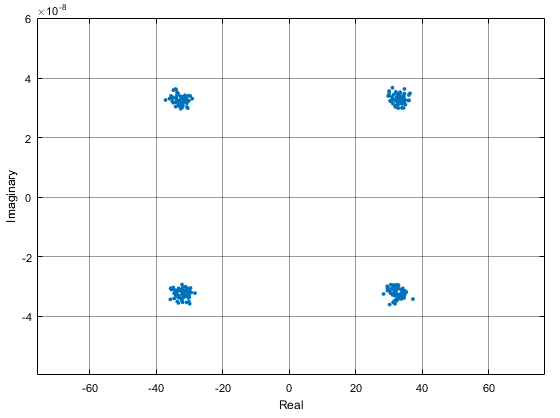
\includegraphics[width=10cm]{./sdf/optical_detection/figures/constelation1.png}
\caption{Simulation of a constelation of 4 states (n = 100)}
\label{fig:constelation}
\end{figure}
%
We see that the measurements made groups in certain regions. Each of this groups is centered in the expected value $(\braket{\textrm{X}}, \braket{\textrm{Y}})$ of one the generated states. Also, they show some variance, which was tested for various expected number of photons, $\braket{n}$, resulting in figure \ref{fig:variance}:
%
\begin{figure}[H]
\captionsetup{justification=centering}
\centering
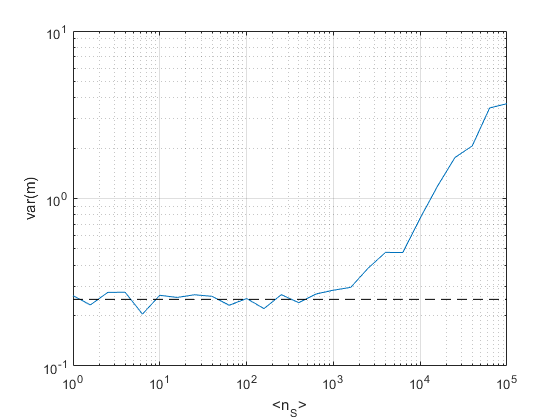
\includegraphics[width=10cm]{./sdf/optical_detection/figures/plot_var_vs_n1.png}
\caption{Simulation of the variance of $m$.\\Local oscillator expected number of photons: $10^4$}
\label{fig:variance}
\end{figure}
%
It was expected that the variance should independent of the input's signal number of photons. Plot \ref{fig:variance} shows that for low values of $n_S$, the simulation is in accordance with the theoretical prevision, with $\textrm{Var(X)} = \textrm{Var(Y)} = \frac{1}{4}$ . For large values of $n_S$, when the number of photons is about the same has the local oscillator, the quantum noise variance starts to grow proportionally to $n_S$, in accordance with the non approximated calculation of quantum noise (eq. \ref{eq:noise}).\\
\\
{\bf Noise Variance with LO power Simulation}\\
The following plot shows the behavior of current noise variance $\braket{(\Delta i)^2}$ with local oscilator power, $P_{LO}$:
%
%
\begin{figure}[H]
	\centering
	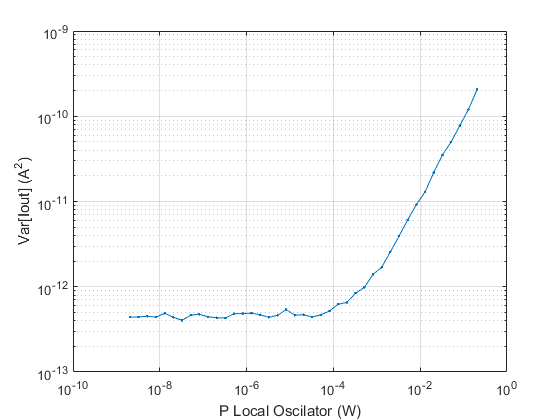
\includegraphics[width=10cm]{./sdf/optical_detection/figures/power_plot.png}
	\caption{Output current variance in function of LO power.}
	\label{fig:variance_lo_power}
\end{figure}
%
%
We see that for low LO power, the dominant noise is the thermal contribution, but for higher power, quantum noise dominates, growing proportionally to $P_{LO}$. This in accordance with equation \ref{eq:var_m}\\
%
%
%
%
\subsection{Experimental Analysis}
%
In this section, we will test experimentally the setups discussed in section \ref{subsec:intro}.
%
This comparison between the theoretical and experimental results will require a high degree of precision from the devices used in these setups. Therefore, the correct characterization of these devices must be the starting point of this experimental phase.
One of the most fundamental components is the photodetector, which performs the signal's conversion from the optical domain into the electrical domain.
%
\subsubsection{Thorlabs detector}
%
The detector used in the laboratory is the Thorlabs PDB 450C. This detector consists of two well-matched photodiodes and a transimpedance amplifier that generates an output voltage (RF OUTPUT) proportional to the difference between the photocurrents of the photodiodes.\\
Additionally, the unit has two monitor outputs (MONITOR+ and MONITOR-) to observe the optical input power level on each photodiode separately.
\cite{thorlabs}
%
\begin{figure}[H]
	\centering
	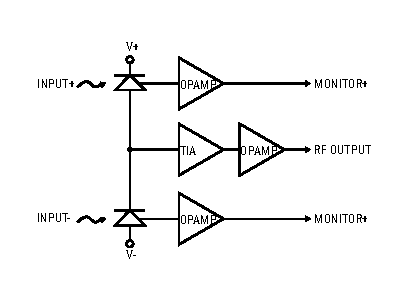
\includegraphics[width=10cm]{./sdf/optical_detection/figures/thorlabs-circuit.pdf}
	\caption{Functional block diagram of the PDB 450C Thorlabs detector \cite{thorlabs}}
	\label{fig:photodetector-circuit}
\end{figure}
%
\noindent
Figure \ref{fig:photodetector-circuit} shows a functional block diagram of the photodetector, in which the TIA (transimpedance amplifier) is an opamp-based current to voltage conversion amplifier.
In contrast to the photodiode's non-linear voltage response to incident light, it's current response is linear.
%\footnote{http://www.ti.com/lit/an/sboa035/sboa035.pdf, p.1}.
To take advantage of this linear response, the TIA is used to perform the conversion of the difference of currents between the two photodiodes into a voltage proportional to that same difference.
%\footnote{http://www.cypress.com/file/131966/download}.
Various of those parameters can be readly extracted from the device's manual, which are presented in the following tables and plots.\\
%
%
%++ ITEMS DO PROF ++
%- responsividade do pin1 e do pin2
%- ganho do meu amplificar OPAMP
%- largura de banda
%- forma do filtro, espectro do filtro
%- ruído térmico, no braço superior, no braço intermédio e no braço inferior
%
%
\begin{table}[H]
	\centering
	\begin{tabulary}{1.0\textwidth}{|L|L|}
		\hline
		\textbf{Parameter}		& \textbf{Value}\\
		\hline
		Max Responsivity		& 1.0 A/W\\
		\hline
	\end{tabulary}
	\caption{Thorlabs PDB450C PIN parameters}
	\label{table:thorlabs}
\end{table}

\begin{table}[H]
	\centering
	\begin{tabulary}{1.0\textwidth}{|L|L|}
		\hline
		\textbf{Parameter}		& \textbf{Value}\\
		\hline
		Bandwidth (-3dB)		& 1 MHz\\
		\hline
		Voltage Gain			& 10 V/mW @ peak responsivity\\
		\hline
		Voltage Noise (RMS)		& <180 \textmu V (RMS)\\
		\hline
	\end{tabulary}
	\caption{Thorlabs PDB450C MONITOR +/- output parameters}
	\label{table:thorlabs}
\end{table}
%
%\noindent
%The manual also contains plots of the response in function of the input's signal frequency, for all the photodetector's outputs.
%Plot \ref{plot:freq-response-monitor} shows the response curves for the two MONITOR outputs.
%
\begin{figure}[H]
	\centering
	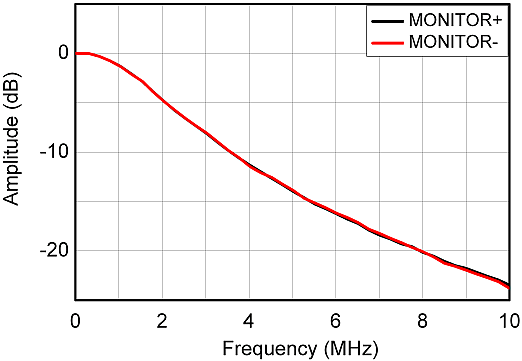
\includegraphics[width=8cm]{./sdf/optical_detection/figures/thorlabs-manual-gain-spec-monitor.png}
	\caption{MONITOR +/- output response with frequency. \cite{thorlabs}}
	\label{plot:freq-response-monitor}
\end{figure}
%
\noindent
The parameters of the RF OUTPUT have 5 values each, corresponding to the 5 gain settings of the TIA.
%
\begin{table}[H]
	\centering
	\begin{tabulary}{1.0\textwidth}{|l|cccccc|}
		\hline
		\textbf{Parameter}					& \multicolumn{6}{l|}{\textbf{Values}}\\
		\hline
		Bandwidth (-3dB)					& $150$  & $45$   & $4$    & $0.3$  & $0.1$  &MHz\\
		\hline
		Transimpedance Gain					& $10^3$ & $10^4$ & $10^5$ & $10^6$ & $10^7$ &V/A\\
		\hline
		Conversion Gain						& $10^3$ & $10^4$ & $10^5$ & $10^6$ & $10^7$ &V/W\\
		\hline
		Overall Output Voltage Noise (RMS)	& $0.50$ & $0.80$ & $1.0$  & $1.1$  & $2.0$  &mV\\
		\hline
	\end{tabulary}
	\caption{Thorlabs PDB450C RF OUTPUT parameters}
	\label{table:parameters-rf}
\end{table}
%
\begin{figure}[H]
	\centering
	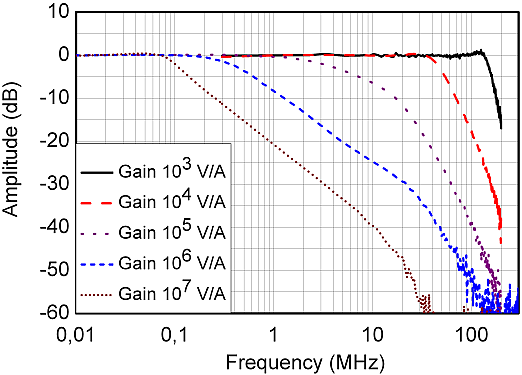
\includegraphics[width=8cm]{./sdf/optical_detection/figures/thorlabs-manual-gain-spec-rf.png}
	\caption{RF output response with frequency, for various gain values. \cite{thorlabs}}
	\label{plot:freq-response-rf}
\end{figure}
%
%
%
%

\subsubsection{Data analysis}
%
For each configuration of amplitude and frequency of the input signal, the photodetector output voltage is collected by the Digital Oscilloscope during a time interval and saved in a data file. The data consists on a sequence of pulses and it's analysis will be focused on the samples with equal phase. The steps will be the following
%
\begin{enumerate}
\item For each phase value, the average and variance of the samples with the same phase is calculated;
\item The representative amplitude and variance for the present configuration will be the obtained from the middle of the maximum plateau.
\end{enumerate}
%
%
%
%
To confirm the theoretical results obtained in section \ref{subsec:intro}, two experimental setups will be created. In the first experiement, we will study quantum noise in the single homodyne detection. The experimental setup will be based on the paper \cite{chi2011balanced}. In the second experiment, we will study quantum noise in the double homodyne detection setup, which will be basically an extension of the single homodyne detection setup.\\
\\
\subsubsection{Single homodyne detection}
%
To keep the experiment simple and avoid extra sources of noise, we will avoid using black boxes wich have complicated inner workings, having a preference in using simple components, as shown in fig. \ref{fig:experimental_homodyne_setup}:
\\
\begin{figure}[H]
	\centering
	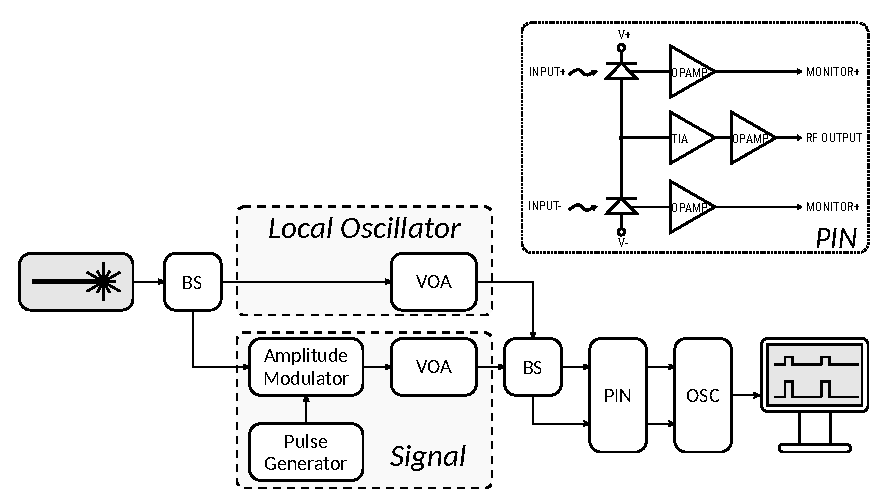
\includegraphics{./sdf/optical_detection/figures/scheme_experimental.pdf}
	\caption{Experimental setup}
	\label{fig:experimental_homodyne_setup}
\end{figure}
%
%
Material list
\begin{table}[H]
	\centering
	\begin{tabulary}{1.0\textwidth}{|L|L|l|}
		\hline
		\textbf{Device}		& \textbf{Description}\\
		\hline
		Local Oscillator	& Yenista OSICS Band C/AG\\
		\hline
		BS					& Beam Splitter\\
		\hline
		Pulse Generator		& HP 8116A Pulse Generator\\
		\hline
		Amplitude Modulator	& Mach Zehnder SDL OC 48\\
		\hline
		VOA					& Eigenlicht Power Meter 420\\
		\hline
		VOA					& Thorlabs VOA 45-APC\\
		\hline
		PIN					& Thorlabs PDB 450C\\
		\hline
		ADC					& Picoscope 6403D\\
		\hline
	\end{tabulary}
\end{table}
%
A single laser is splitted and used as the source for the signal (S) and the local oscillator (LO). The signal beam is pulsed and highly attenuated. The local oscillator is also attenuaded, but not pulsed. The signal and local oscillator interfere in a Beam Splitter originating two beams which are then converted to voltages in the PIN. These voltages are read in the Digital Oscilator (OSC) and collect in the computer. In the post processing phase, the quantum noise is measured by applying a difference between the two beams and measuring it's variance.
\\
The second stage of the experiment will be very similar to the first one, in which the signal and local oscillator branches will be divided. One of the new branches of the local oscilator will suffer a phase delay of $\pi/2$, in order to measure the quadrature component of the incoming signal.\\
%%
%%

\subsection{Comparative analysis}
%
%WARNING -- OLD DATA --\\
%
Given the theoretical, simulated and experimental frameworks, we will now compare the results obtained by each of them.
\\
%
\begin{figure}[H]
	\begin{subfigure}{.5\textwidth}
		\centering
		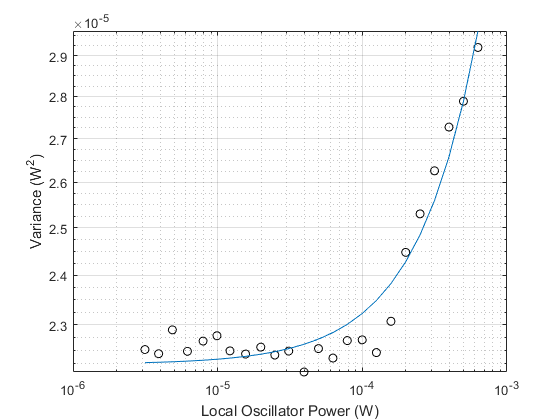
\includegraphics[width=.8\linewidth]{./sdf/optical_detection/figures/noise_exp_channel1.png}
		\caption{$X$ quadrature}
		\label{fig:noise-exp-1}
	\end{subfigure}%
	\begin{subfigure}{.5\textwidth}
		\centering
		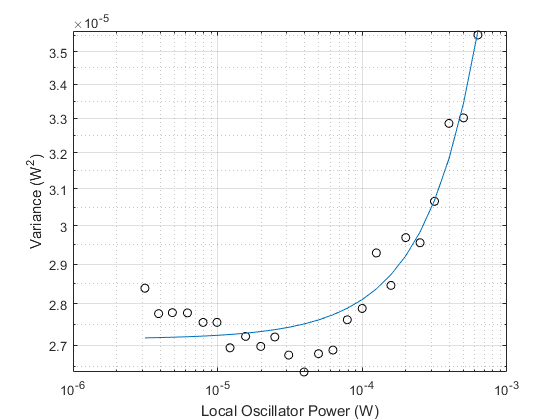
\includegraphics[width=.8\linewidth]{./sdf/optical_detection/figures/noise_exp_channel3.png}
		\caption{$Y$ quadrature}
		\label{fig:noise-exp-3}
	\end{subfigure}
	\captionsetup{justification=centering}
	\caption{Noise variance dependency with local oscilator power for two different quadratures. Experimental vs fitted data.}
\end{figure}
%
Figures $\ref{fig:noise-exp-1}$ and $\ref{fig:noise-exp-3}$ show measurements of total noise for two different quadratures. For low power of LO, the noise variance flutuates around a constant value. For high power of LO, $(P_{LO}>10^{-4}W)$, the variance of noise shows an increasing trend roughly proportional to $P_{LO}^2$. The polynomial fittings confirm this trend, showing a degree 2 coefficient much larger than the degree 1 coefficient
%
\begin{equation}
\textrm{Var}_X = 2.22 \!\! \times \!\! 10^{-5} + 9.6 \!\! \times \!\! 10^{-3} P_{LO} + 3.40 P_{LO}^2
\end{equation}
\begin{equation}
\textrm{Var}_Y = 2.71 \!\! \times \!\! 10^{-5} + 8.9 \!\! \times \!\! 10^{-3} P_{LO} + 7.25 P_{LO}^2
\end{equation}
%
The expected growth should be proportional to $P_{LO}$, but the RIN noise, originated by the electric apparatus, which grows quadratically with the power, is dominating the noise amplitude for large $P_{LO}$.\\
We see that both the simulation and experimental data display a similar behaviour, but the quadratic growth of noise for large $P_{LO}$ was not predicted in the simulations.\\



%
%
\subsection{Known problems}
%

 \fi
\ifdefined\bpsk         \input{./sdf/bpsk_system/bpsk_system} \fi
\ifdefined\m            \clearpage
\section{M-QAM Transmission System}

\begin{tcolorbox}	
	\begin{tabular}{p{2.75cm} p{0.2cm} p{10.5cm}} 	
		\textbf{Student Name}  & & Andoni Santos (2018/01/03 - )\\
							   & & Ana Luisa Carvalho (2017/04/01 - 2017/12/31) \\
		\textbf{Goal}          &:& M-QAM system implementation with BER measurement and comparison with theoretical and experimental values.\\
		\textbf{Directory} &:& sdf/m\_qam\_system
	\end{tabular}
\end{tcolorbox}

The goal of this project is to simulate a Quadrature Amplitude Modulation transmission system with M points in the constellation diagram (M-QAM) and to perform a Bit Error Rate (BER) measurement that can be compared with theoretical and experimental values.

%TODO: Verify
M-QAM systems can encode $\log_2 M$ bits per symbol which means they can transmit higher data rates keeping the same bandwidth when compared, for example, to PSK systems. However, because the states are closer together, these systems require a higher singal-to-noise ratio.
The Bit Error Rate (BER) is a measurement of how a bit stream is altered by a transmission system due to noise (among other factors). To study this effect we introduced Additive White Gaussian Noise (AWGN) to model thermal noise at the receiver.

For $M=4$ the M-QAM system can be reduced to a Quadrature Phase Shift Keying system (QPSK) system that uses four equispaced points in the constellation diagram (see figure \ref{fig:const}).

\begin{figure}[h]
	\centering
	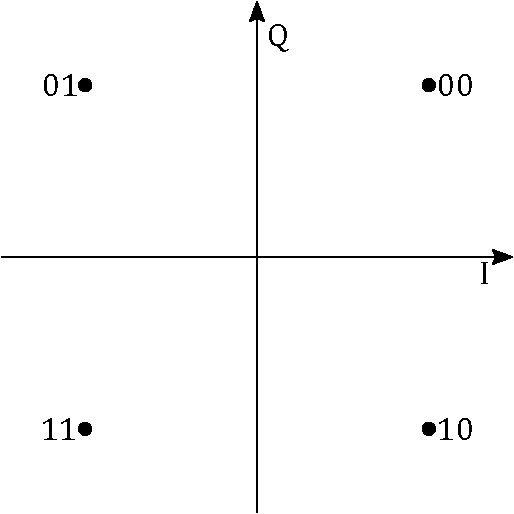
\includegraphics[width=0.5\textwidth]{./sdf/m_qam_system/figures/constellation.pdf}
	\caption{4-QAM constellation points.}
	\label{fig:const}
\end{figure}

%M can take several values: $2, 4, 16, 32, ...$. The first two correspond to BPSK and QPSK modulation, respectively.

\subsection{Theoretical Analysis}

M-QAM is a modulation scheme that takes advantage of two sinusoidal carriers with a phase difference of $\pi/2$. The resultant output consists of a signal with both amplitude and phase variations. The two carriers, referred to as I (In-phase) and Q (Quadrature), can be represented as

\begin{align}
	I(t)=A(t)\cos(\phi t) \\
	Q(t)=A(t)\sin(\phi t)
\end{align}
which means that any sinusoidal wave can be decomposed in its I and Q components:

\begin{align}
	A\cos(\omega~t+\phi)&=A\left(\cos(\omega~t)\cos(\phi)-\sin(\omega~t)\sin(\phi)\right) \\
	&=I\cos(\omega~t)-Q\sin(\omega~t),
\end{align}
where we have used the expression for the cosine of a sum and the definitions of I and Q.



For the particular case of $M=4$, considering there is no crosstalk or interference between the Q and I components, the signal can be treated as a pair of independent BPSK systems, one for the in-phase component and another for the quadrature component.
Using Gray coding, adjacent symbols differ by only one bit. As such, an error in a single component leads to a single bit error.
This means that the probability of an error in bit detection is independent among components, as there is no crosstalk or interference. That being the case, the bit error rate can be calculated for the BPSK case.

%Considering a signal with amplitude $A$ sampled at the signal peak with no inter-symbol interference, and affected by noise with variance $n_0/2$, the sampled value will be a Gaussian random variable with mean $\pm A$ and variance $n_0/2$. Thus, the probability of error is given by the probability that the value is affected by a deviation greater than $m$.

Let the $s(t)$ be the signal sampled at a given instant $t$ for either the in-phase or quadrature component, $A(t)$ be the component corresponding to the transmitted signal with value equal to $\pm A$, depending on whether the transmitted signal was 1 or 0, and $n(t)$ the component associated with the Gaussian white noise with variance $n_0/2$, such that

\begin{equation}\label{eq:sigAmpNoise}
s(t) = A(t) + n(t)
\end{equation}

\begin{figure}[H]
	\centering
	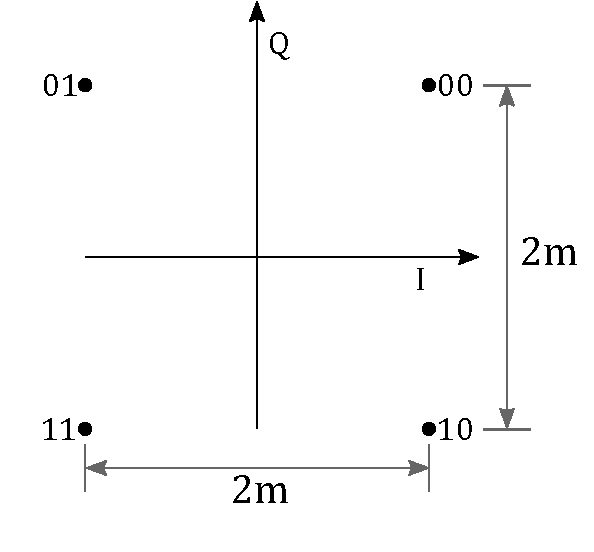
\includegraphics[width=0.5\textwidth]{./sdf/m_qam_system/figures/constellation_d.pdf}
	\caption{The relation between $m$ and the distance between constellation points.\label{fig:const_2m}}
\end{figure}

In this case, assuming the absence of inter-symbol interference, $s(t)$ will be a Gaussian random variable with average value of $\pm A$, depending on what signal was transmitted, and variance equal to $n_0/2$. In this case, using the constellation from Figure~\ref{fig:const_2m}, with a decision boundary halfway between $A$ and $-A$, an error occurs in two situations: when the a 0 is transmitted but a 1 is identified, or a 1 is transmitted and a 0 is identified. These mistakes happen when the perturbation in the signal due to noise is enough to push the value beyond the decision boundary. These situations are shown in Figures~\ref{fig:gauss} and~\ref{fig:gausserr}, by the colored area under the curve.

\begin{figure}[H]
	\centering
	\centering
	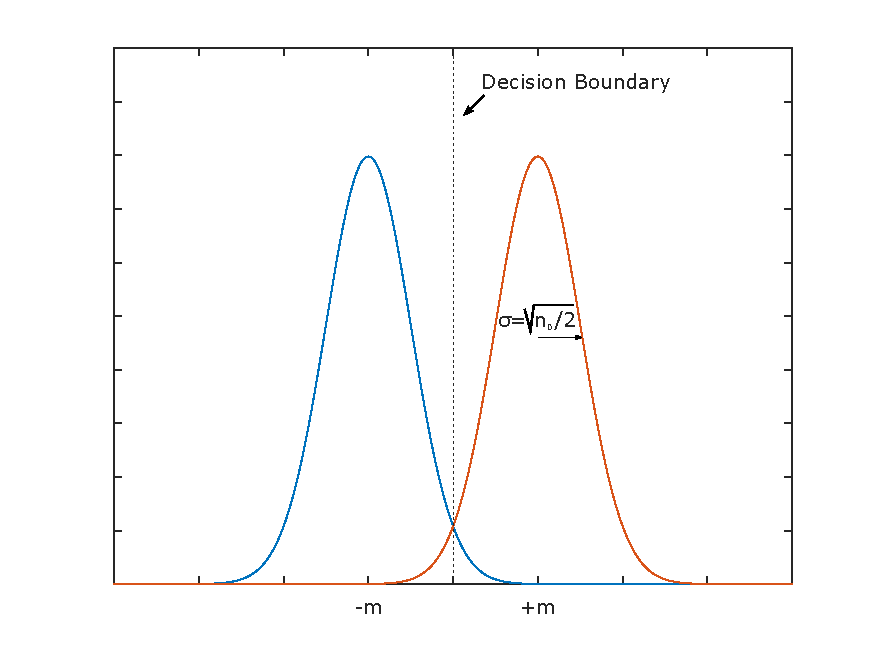
\includegraphics[ width=0.8\textwidth]{./sdf/m_qam_system/figures/gaussians.pdf}
	\caption{Probability density functions for $s(t) = m(t) + n(t)$, with $m(t)=\pm m$ and $n(t)$ as a Gaussian variable.}
	\label{fig:gauss}
\end{figure}

\begin{figure}[H]
	\centering
	\begin{subfigure}{.5\textwidth}
		\centering
		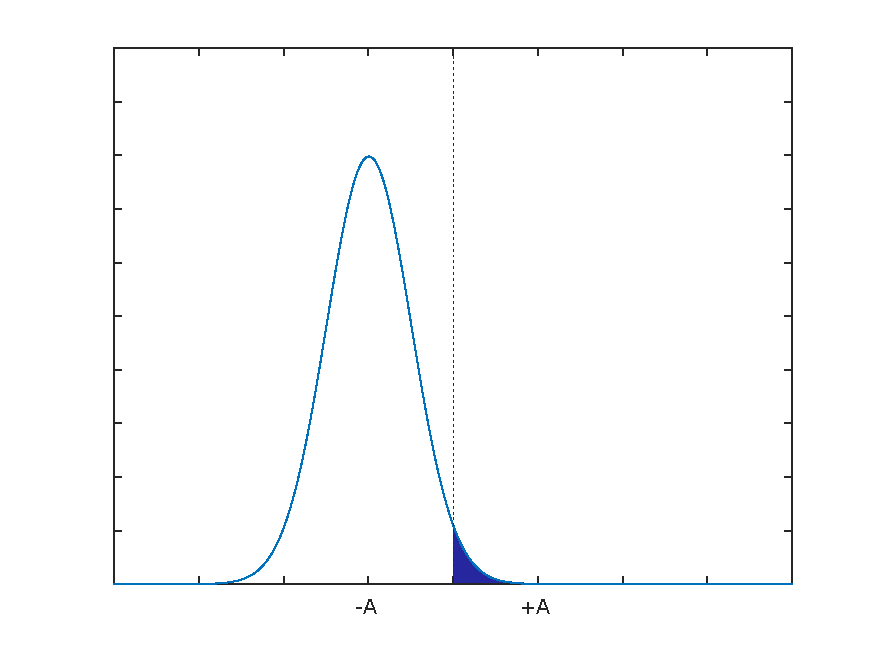
\includegraphics[clip, trim=1cm 0cm 1cm 0cm,width=\textwidth]{./sdf/m_qam_system/figures/gaussian_error_2.pdf}
	\end{subfigure}%
	\begin{subfigure}{.5\textwidth}
		\centering
		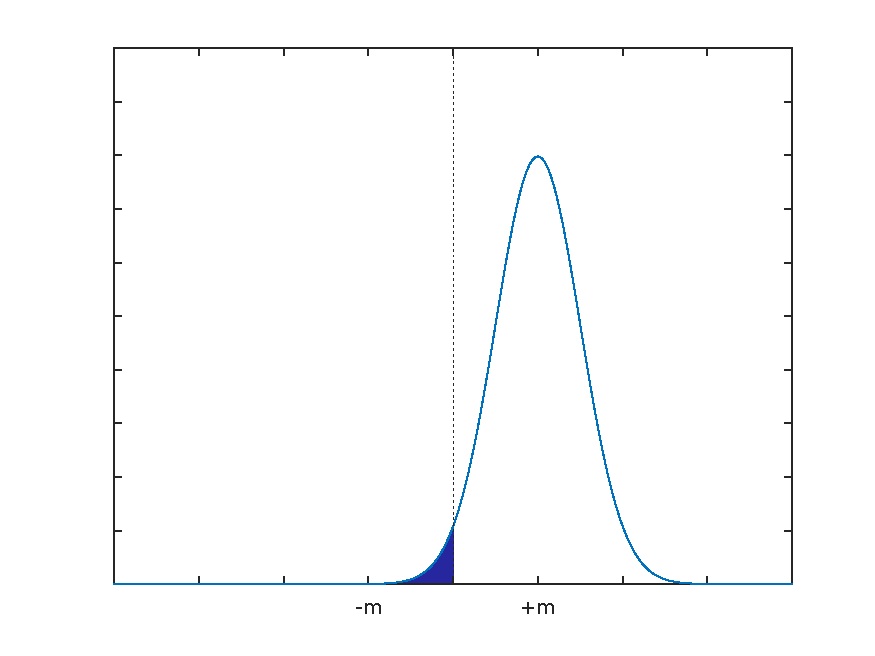
\includegraphics[clip, trim=1cm 0cm 1cm 0cm,width=\textwidth]{./sdf/m_qam_system/figures/gaussian_error.pdf}
	\end{subfigure}
	\caption{The area below the curves represents the probability of error for each transmitted bit.}
	\label{fig:gausserr}
\end{figure}

The probability of bit error can be expressed as:

\begin{equation}
P_{be} = P_0 P_{e0} + P_1 P_{e1}
\end{equation}

With equal probability for both bits, and considering the constellation's symmetry

\begin{equation}\label{eq:berMQAM}
P_{be} =  Q\left({\frac{A}{n_0}}\right) = \frac{1}{2} \text{erfc}\left({\frac{A}{N_0}}\right)
\end{equation}


%\begin{equation}
%P_b= Q\left(\sqrt{\frac{E_b}{n_0}}\right) = \frac{1}{2} erfc\left(\sqrt{\frac{E_b}{2 n_0}}\right).
%\end{equation}

%\begin{equation}\label{eq:berBPSK}
%P_{BE}= Q\left({\sqrt{\frac{2 E_b}{N_0}}}\right) = \frac{1}{2} \text{erfc}\left({\sqrt{\frac{ E_b}{N_0}}}\right).
%\end{equation}

%\begin{equation}\label{eq:berBPSK}
%BER= Q\left({G_{ele}\sqrt{\frac{2 P_L P_S}{n_0}}}\right) = \frac{1}{2} \text{erfc}\left({G_{ele}\sqrt{\frac{P_L P_S}{n_0}}}\right).
%\end{equation}

with


\begin{eqnarray}
&A &= G_{ele} \sqrt{P_L P_S} \\
&N_0 &= \sqrt{\frac{n_0}{2}}
\end{eqnarray}
%\begin{equation}\label{eq:berBPSK}
%BER= Q\left({G_{ele}\sqrt{\frac{2 P_L P_S}{n_0}}}\right) = \frac{1}{2} \text{erfc}\left({G_{ele}\sqrt{\frac{P_L P_S}{n_0}}}\right).
%\end{equation}

\noindent where $P_L$ is the local oscillator power, $P_S$ is the optical signal power, $G_{ele}$ is the gain in the transimpedance amplifier and $n_0$ is the noise spectral density. Figure~\ref{fig:const_2m} shows the relation between the constellation points and $A$. $N_0$ will be the standard deviation of the sampled values.





The symbol error rate however is not the same, as it depends on both bits being correctly detected. The probability of both bits being correctly detected is:

\begin{equation}
P_C = (1 - P_{be})^2
\end{equation}

From this, the probability of symbol error is:

\begin{eqnarray}
&P_s &= 1-P_C =\nonumber \\
&	   &= 1 - \left(1 - Q \left({\frac{A}{n_0}}\right)\right)^2 = \nonumber \\
&	   &= 2 Q\left({\frac{A}{n_0}}\right)\left[1-\frac{1}{2} Q \left({\frac{A}{n_0}}\right)\right]
\end{eqnarray}

%The bit error rate is then equal to the probability of the phase falling outside the correct detection range in a given component due to noise,


%Exact solutions for the probability of symbol and bit errors exist only for $M=4$.

%As previously mentioned, for $M=4$ the system is reduced to a QPSK system. Knowing that the AWGN is independent

%For the cases of $M>4$, an aproximation can be used.
%The probability of symbol error, $P_s$, in coherent M-PSK demodulation with AWGN can be aproximated by
%
%\begin{equation}
%	P_s=2~Q\left(\sqrt{2~\log_2 M \left(\frac{E_b}{n_0}\right)\sin^2\frac{\pi}{M}}\right)
%\end{equation}
%where $E_b$ is the energy of one bit, $n_0$ is the noise power and the function $Q$ is defined as
%\begin{equation}
%	Q(x)=\frac{1}{2} erfc\left(\frac{x}{\sqrt{2}}\right).
%	\label{eq:Ps}
%\end{equation}
%
%It is worth noting that this aproximation is only valid for high SNR values. The probability of bit errors for $M>4$ can now be estimated, as it is related to $P_s$ by
%
%\begin{equation}
%	P_b=\frac{1}{\log_2 M}P_s.
%	\label{eq:Pb}
%\end{equation}
%
%For QPSK we get, using $M=4$ in equations \ref{eq:Ps} and \ref{eq:Pb},
%\begin{equation}
%	P_b= 2 Q\left(\sqrt{\frac{2~E_b}{n_0}}\right) = erfc\left(\sqrt{\frac{E_b}{n_0}}\right).
%\end{equation}
%
%The exact probability bit error for $M=4$ are

%The Bit Error Rate curve given by~\eqref{eq:berBPSK} is plotted in figure \ref{fig:QPSK_th_curve} as a function of the optical signal power for $N_0=10^{-6}$, $P_L = 0~dBm$ and $G_{ele} = 10^3$.

%\begin{figure}[h]
%		\centering
%		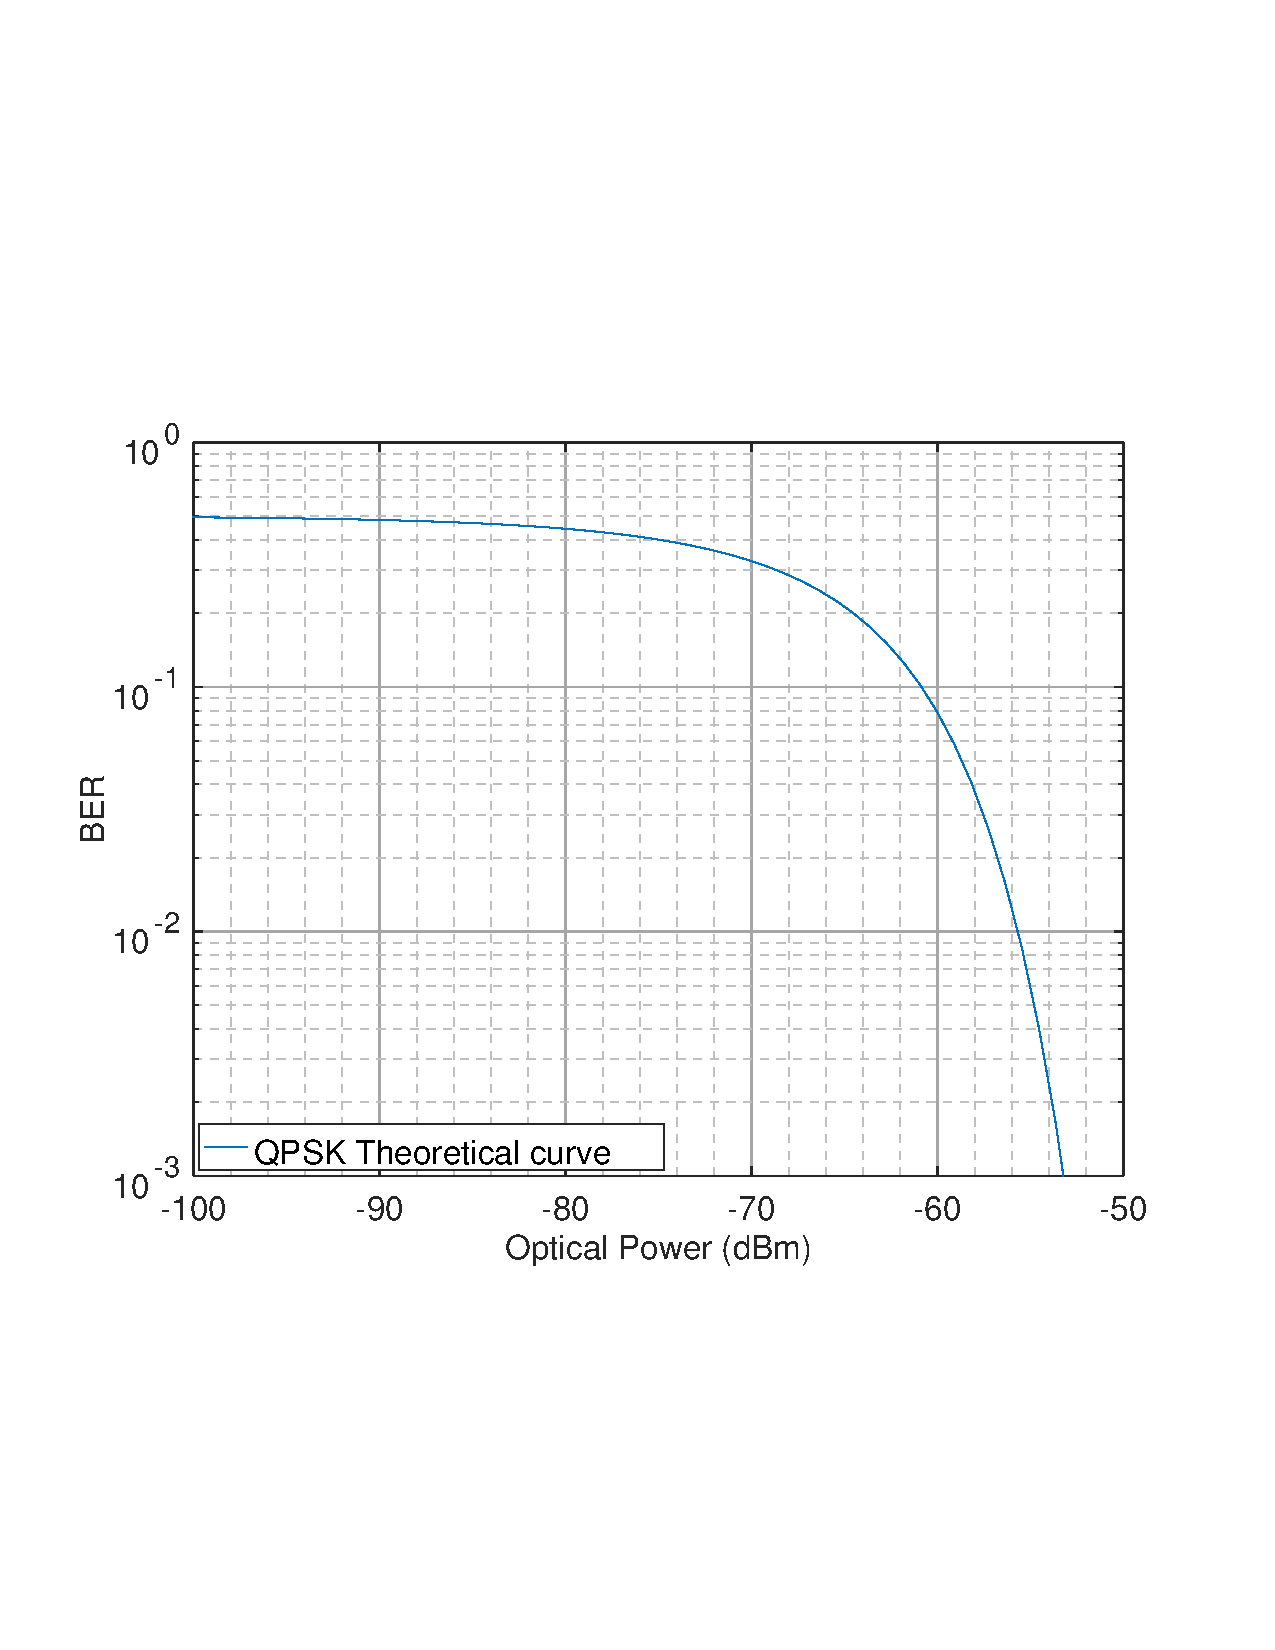
\includegraphics[clip, trim=2cm 6cm 2cm 6cm, width=0.7\textwidth]{./sdf/m_qam_system/figures/BER_QPSK_theory_20180119.pdf}
%		\caption{QPSK theoretical BER values as a function of the output optical power in dBm.}
%		\label{fig:QPSK_th_curve}
%\end{figure}

It is possible to further decrease the error rate by using a matched filter before sampling the signal. The resulting signal will still have Gaussian noise, but the signal-to-noise ratio will be greatly improved. This can be achieved, for instance by using a root-raised cosine filter at the pulse shaper and another one before the sampler. Inter-symbol interference will still be null as it is equivalent to a raised cosine filter, where half the filtering is done on the transmitter side (while pulse-shaping) and the other half is done on the receiver side, before sampling.

%As the constellation remains the same, the expression to calculate the BER is similar, but replacing the values of $m$ and $N_0$ of Equation~\eqref{eq:berMQAM} by those corresponding to the signal at the output of the filter, which can be calculated as:
Considering a signal similar to the one described by Equation~\ref{eq:sigAmpNoise}, the output of the matched filter receiver will be~\cite{mischasch}:

\begin{eqnarray}
&s_{mf} (t) &= \int_{0}^{T} s(t)\cos(\omega_0 t ) dt\nonumber\\ 
&	       &= \int_{0}^{T} m(t) \cos(\omega_0 t ) dt + \int_{0}^{T} n(t) \cos(\omega_{0} t ) dt
\end{eqnarray}

In the case of QPSK with m=4, both the quadrature and in-phase components have $m(t) = \pm A$. The values that replace $m$ and $N_0$ in Equation~\ref{eq:berMQAM} become:

\begin{eqnarray}
&m_{mf} &= \frac{A T}{2}\\
&N_{mf} &= \sqrt{\sigma_o^2} = E(n_o^2) = \sqrt{\frac{n_0 T}{4}}
\end{eqnarray}

% TODO: ADD noise and signal calculation for mf

The optimal BER that can be obtained by using matched filtering is then given by:

\begin{eqnarray}\label{eq:berBPSK}
&P_{be} &= \frac{1}{2} \text{erfc}\left({\frac{AT/2}{\sqrt{2} N_{mf}}}\right)\nonumber\\
&	    &= \frac{1}{2} \text{erfc}\left(\sqrt{{\frac{A^2T}{2 n_0}}}\right)\\
&	    &= \frac{1}{2} \text{erfc}\left(\sqrt{{\frac{E_b}{n_0}}}\right)\nonumber
\end{eqnarray}

with

\begin{eqnarray}
%&m_{mf} &= \frac{1}{2} T G_{ele} \sqrt{P_L P_S} \\
&E_b &= \frac{A^2 T}{2} \\
\end{eqnarray}

\noindent where T is the symbol period.
Figure~\ref{fig:QPSK_th_curves} show the curves for both these equations, in the case where  $n_0=10^{-6}$, $P_L = 0~dBm$ and $G_{ele} = 10^3$.
%Here, $T$ is the symbol period. 


\begin{figure}[H]
		\centering
		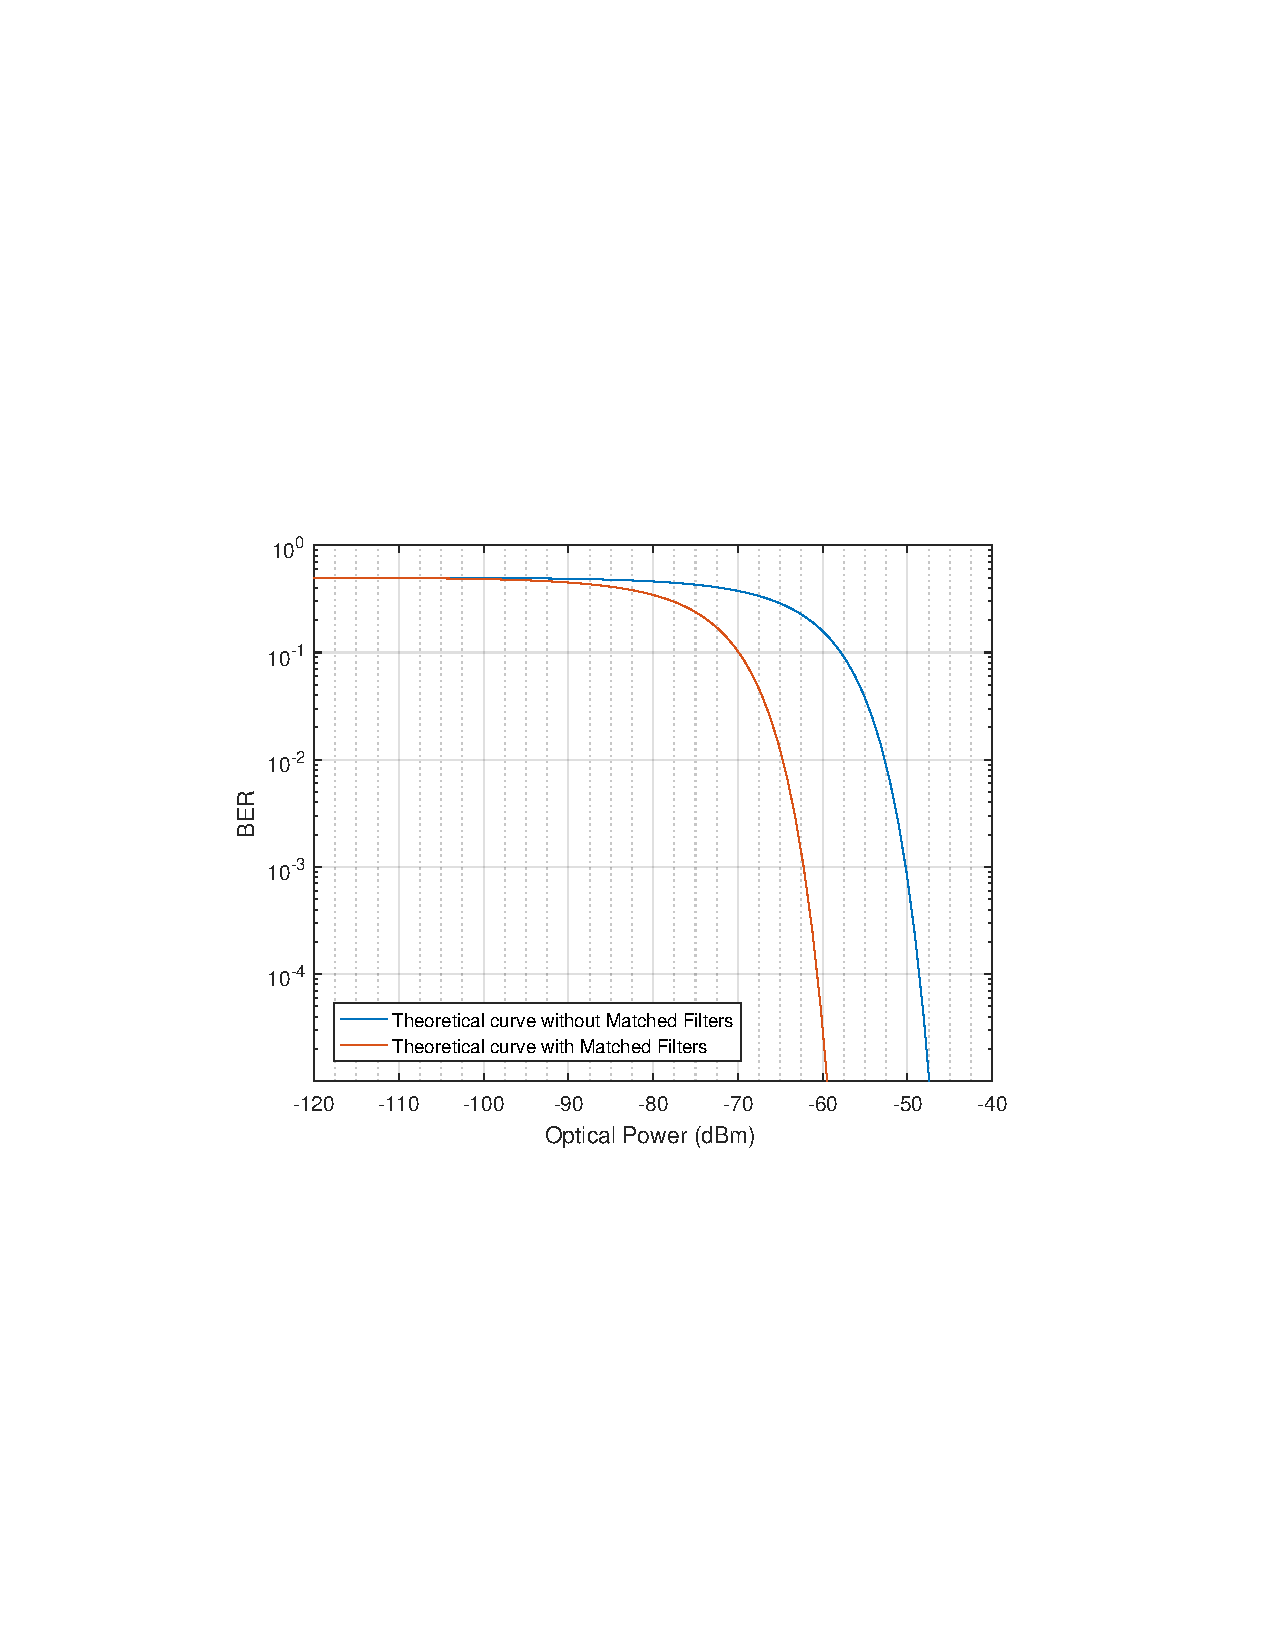
\includegraphics[clip, trim=4cm 8cm 4cm 8cm, width=0.7\textwidth]{./sdf/m_qam_system/figures/teor_BER_curves.pdf}
		\caption{QPSK theoretical BER values as a function of the output optical power in dBm.\label{fig:QPSK_th_curves}}	
\end{figure}

Figure~\ref{fig:QPSK_th_curves} shows the two theoretical curves for QPSK. The blue one is for QPSK without matched filtering and the red one is using root-raised-cosine for matched filtering, which provides optimum transmission. As the use of root-raised-cosine for matched filtering maximizes the signal-to-noise ratio to its optimal value, it allows achieving the same BER with much lower optical power. On the blue curve, on the other hand, the sampling is affected by the full effect of the random noise, as there is no filtering at the receiver. Because of this, a higher optical power is required to achieve a similar BER.


It's worth noting that these equations are only valid for M=4, as in that case the system is similar to QPSK with a 4 point constellation. For $M > 4$ a different approach is required.


\subsection{Simulation Analysis}

\begin{figure}[h]
	\centering
	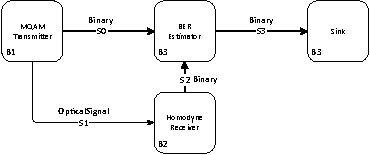
\includegraphics[width=0.8\textwidth]{./sdf/m_qam_system/figures/simulation_mqam}
	\caption{Schematic representation of the MQAM system.}\label{MQAM_system_block_diagram}
\end{figure}

The M-QAM transmission system is a complex block of code that simulates the modulation, transmission and
demodulation of an optical signal using M-QAM modulation.
It is composed of four blocks: a transmitter, a receiver, a sink and a block that performs a Bit Error Rate (BER) measurement. The schematic representation of the
system is presented in figure \ref{MQAM_system_block_diagram}.
	
\paragraph{Current state:} The system currently being implement is a QPSK system (M=4).

\paragraph{Future work:} Extend this block to include other values of M.

\subsection*{Functional description}

A complete description of the M-QAM transmitter and M-QAM homodyne receiver blocks can be found in the \textit{Library} chapter of this document as well as a detailed description of the independent blocks that compose these blocks.

The M-QAM transmitter generates one or two optical signals by encoding a binary string using M-QAM modulation. It also outputs a binary signal that is used to perform the BER measurement.

The M-QAM homodyne receiver accepts one input optical signal and outputs
a binary signal. It performs the M-QAM demodulation of the input signal by combining the optical signal with a local oscillator.

The demodulated optical signal is compared to the binary one produced by the transmitter in order to estimate the Bit Error Rate (BER).

The files used are summarized in tables~\ref{tab:sources} and~\ref{tab:headers}. These include all blocks and sub-blocks used and allow for the full operation of the M-QAM system.

\subsection*{Required files}\label{Required files}

\begin{table}[H]
    \centering
    \begin{tabulary}{1.0\textwidth}{|p{7.5cm}|p{5.5cm}|p{1cm}|}
        \hline
        \multicolumn{3}{|c|}{ \textbf{Source Files} } \\
        \hline
        \textbf{File}                      			 & \textbf{Comments} & \textbf{Status} \\ \hline
        add\_20171116.cpp                            &                   & \checkmark \\ \hline
        binary\_source\_20180118.cpp                 &                   & \checkmark \\ \hline
        bit\_error\_rate\_20171810.cpp               &                   & \checkmark \\ \hline
        decoder\_20180118.cpp                        &                   & \checkmark \\ \hline
        discrete\_to\_continuous\_time\_20180118.cpp &                   & \checkmark \\ \hline
        homodyne\_receiver\_20171203.cpp             & $^{1}$			 & \checkmark \\ \hline
        ideal\_amplififer\_20180118.cpp              &                   & \checkmark \\ \hline
        iq\_modulator\_20180118.cpp                  &                   & \checkmark \\ \hline
        local\_oscillator\_20180118.cpp              &                   & \checkmark \\ \hline
        m\_qam\_mapper\_20180118.cpp                 &                   & \checkmark \\ \hline
        m\_qam\_system.cpp                 			 & $^{2}$   		 & \checkmark \\ \hline
        m\_qam\_transmitter\_20180118.cpp            &                   & \checkmark \\ \hline
        netxpto\_20180118.cpp                        & $^{2}$ 			 & \checkmark \\ \hline
        optical\_hybrid\_20180118.cpp                &                   & \checkmark \\ \hline
        photodiode\_old\_20180118.cpp                &                   & \checkmark \\ \hline
        pulse\_shaper\_20180118.cpp                  &                   & \checkmark \\ \hline
        sampler\_20171119.cpp                        &                   & \checkmark \\ \hline
        sink\_20180118.cpp                           &                   & \checkmark \\ \hline
        super\_block\_interface\_20180118.cpp        & $^{2}$ 			 & \checkmark \\ \hline
        white\_noise\_20180118.cpp                   & 					 & \checkmark \\ \hline
    \end{tabulary}

    \caption{$^1$ The library entry is under a different name, \textit{m\_qam\_receiver};\\
    $^2$ No library entry as it is a main or general purpose file, not a specific block. 	 \label{tab:sources}}
\end{table}

\begin{table}[H]
    \centering
    \begin{tabulary}{1.0\textwidth}{|p{7cm}|p{6cm}|p{1cm}|}
        \hline
        \multicolumn{3}{|c|}{ \textbf{Header Files} } \\
        \hline
        \textbf{File}                      & \textbf{Comments} & \textbf{Status} \\ \hline
        add\_20171116.h                            & 			   & \checkmark \\ \hline
        binary\_source\_20180118 .h                &                   & \checkmark \\ \hline
        bit\_error\_rate\_20171810.h               &             & \checkmark \\ \hline
        decoder\_20180118.h                        &                   & \checkmark \\ \hline
        discrete\_to\_continuous\_time\_20180118.h &                   & \checkmark \\ \hline
        homodyne\_receiver\_20171203.h             & $^{1}$          & \checkmark \\ \hline
        ideal\_amplifier\_20180118.h               &                   & \checkmark \\ \hline
        iq\_modulator\_20180118.h                  &                   & \checkmark \\ \hline
        local\_oscillator\_20180118.h              &                   & \checkmark \\ \hline
        m\_qam\_mapper\_20180118.h                 &                   & \checkmark \\ \hline
        m\_qam\_transmitter\_20180118.h            &                   & \checkmark \\ \hline
        netxpto\_20180118.h                        & $^2$ 			   & \checkmark \\ \hline
        optical\_hybrid\_20180118.h                &                   & \checkmark \\ \hline
        photodiode\_old\_20180118.h                &                   & \checkmark \\ \hline
        pulse\_shaper\_20180118.h                  &                   & \checkmark \\ \hline
        sampler\_20171119.h                        &               & \checkmark \\ \hline
        sink\_20180118.h                           &                   & \checkmark \\ \hline
        super\_block\_interface\_20180118.h        & $^2$			   & \checkmark \\ \hline
        white\_noise\_20180118.h                   &                   & \checkmark \\ \hline
    \end{tabulary}
    \caption{$^1$ The library entry is under a different name, \textit{m\_qam\_receiver}\\
    $^2$ No library entry as it is a main or general purpose file, not a specific block. \label{tab:headers}}
\end{table}

%\begin{table}[]
%	\centering
%	\caption{Main system files}
%	\begin{tabular}{|c|c|c|c|ccc}
%		\cline{1-4}
%		\textbf{System blocks} & \textbf{Source file} & \textbf{Header file}  &  \textbf{Status} & \\ \cline{1-4}
%		Main & m\_qam\_system\_sdf.cpp & --- & \checkmark & \\ \cline{1-4}
%		M-QAM transmitter & m\_qam\_transmitter\_20180118.cpp & m\_qam\_transmitter\_20180118.h & \checkmark &  \\ \cline{1-4}
%		M-QAM receiver & homodyne\_receiver\_20180118.cpp & homodyne\_receiver\_20180118.h & \checkmark &  \\ \cline{1-4}
%		Sink & sink\_20180118.cpp & sink\_20180118.h &  \checkmark & \\ \cline{1-4}
%		BER estimator & bit\_error\_rate\_20171810.cpp & bit\_error\_rate\_20171810.h & \checkmark &\\ \cline{1-4}
%	\end{tabular}
%	\label{files_table}
%\end{table}

%\subsection*{Required Files}
%
%The required header and source files needed to run this system are summarized in table \ref{table:files}.
%
%\begin{table}
% 	\centering
% 	\caption{Required files}
% 	\begin{tabular}{|c|c|p{40mm}|c|ccp{40mm}c}
% 		\cline{1-4}
% 		\textbf{Header file} & \textbf{Source file} & \textbf{Description} &  \textbf{Status} & \\ \cline{1-4}
% 		add.h & add.cpp & Adds two signals.  & \checkmark &   \\ \cline{1-4}
% 		binary\_source.h & binary\_source.cpp & Produces a binary sequence. & \checkmark & \\ \cline{1-4}
% 		bit\_error\_rate.h & bit\_error\_rate.cpp & Computes the BER and writes it to a text file. & \checkmark & \\ \cline{1-4}
% 		discrete\_to\_continuous\_time.h & discrete\_to\_continuous\_time.cpp & Converts a signal from discrete in time to continuous in time. & \checkmark & \\ \cline{1-4}
% 		homodyne\_receiver.h & m\_qam\_homodyne\_receiver.cpp & & \\ \cline{1-4}
% 		ideal\_amplifier.h & ideal\_amplifier.cpp & Amplifies the signal. & \checkmark & \\ \cline{1-4}
% 		iq\_modulator.h & iq\_modulator.cpp & Divides the signal in its quadrature and in phase components & \checkmark &\\ \cline{1-4}
% 		local\_oscillator.h & local\_oscillator.cpp & & & \checkmark &\\ \cline{1-4}
% 		m\_qam\_mapper.h & m\_qam\_mapper.cpp & Maps the signal using the defined constellation & \checkmark & \\ \cline{1-4}
% 		m\_qam\_transmitter.h & m\_qam\_transmitter.cpp & & \checkmark & \\ \cline{1-4}
% 		netxpto.h & netxpto.cpp & General class that contains definition from signals and buffers. & \checkmark &\\ \cline{1-4}
% 		optical\_hybrid.h & optical\_hybrid.cpp & Implements an optical hybrid. & \checkmark & \\ \cline{1-4}
% 		photodiode\_old.h & photodiode\_old.cpp & Pair of photodiodes and current subtraction. & \checkmark & \\ \cline{1-4}
% 		pulse\_shaper.h & pulse\_shaper.cpp & Electrical filter. & \checkmark &\\ \cline{1-4}
% 		sampler\_20171119.h & sampler\_20171119.cpp & Samples the signal. & \checkmark &\\ \cline{1-4}
% 		sink.h & sink.cpp & Deletes signal. & \checkmark & \\ \cline{1-4}
% 		super\_block\_interface.h & super\_block\_interface.cpp & & \checkmark &\\ \cline{1-4}
% 		white\_noise.h & white\_noise.cpp & Generates white gaussian noise. & \checkmark &\\ \cline{1-4}
% 	\end{tabular}
% 	\label{table:files}
%\end{table}
\pagebreak
\subsection*{Input Parameters}

%The system accepts several input parameters that can be defined by the user. These are described in table \ref{table:in_par}.

\begin{table}[H]
	\centering
	\caption{Input parameters}
	\begin{tabular}{|c|c|p{70mm}|ccp{70mm}}
		\cline{1-3}
		\textbf{Parameter} & \textbf{Type} & \textbf{Description} &    \\ \cline{1-3}
		numberOfBitsGenerated & t\_integer & Determines the number of bits to be generated by the binary source  &    \\ \cline{1-3}
		samplesPerSymbol & t\_integer & Number of samples per symbol &    \\ \cline{1-3}
		prbsPatternLength & int & Determines the length of the pseudorandom sequence pattern (used only when the binary source is operated in \textit{PseudoRandom} mode) &    \\ \cline{1-3}
		bitPeriod & t\_real & Temporal interval occupied by one bit &    \\ \cline{1-3}
		rollOffFactor\_shp & t\_real & Parameter of the pulse shaper filter &    \\ \cline{1-3}
		rollOffFactor\_out & t\_real & Parameter of the output filter &    \\ \cline{1-3}
		shaperFilter & enum & Type of filter used in Pulse Shaper &    \\ \cline{1-3}
		outputFilter & enum & Type of filter used in output filter &    \\ \cline{1-3}
		seedType & enum & Method of seeding noise generators &    \\ \cline{1-3}
		seedArray & array<int,2> & Seeds to initialize noise generators &    \\ \cline{1-3}
		signalOutputPower\_dBm & t\_real & Determines the power of the output optical signal in dBm &  \\ \cline{1-3}
		numberOfBitsReceived & int &   Determines when the simulation should stop. If $-1$ then it only stops when there is no more bits to be sent&   \\ \cline{1-3}
		iqAmplitudeValues & vector<t\_iqValues> & Determines the constellation used to encode the signal in IQ space &    \\ \cline{1-3}
		symbolPeriod & double & Given by bitPeriod/samplesPerSymbol &    \\ \cline{1-3}
		localOscillatorPower\_dBm & t\_real & Power of the local oscillator &    \\ \cline{1-3}
		responsivity & t\_real & Responsivity of the photodiodes (1 corresponds to having all optical power transformed into electrical current) &    \\ \cline{1-3}
		amplification & t\_real & Amplification provided by the ideal amplifier &    \\ \cline{1-3}
		noiseAmplitude & t\_real & Amplitude of the white noise &    \\ \cline{1-3}
		samplesToSkip & t\_integer & Number of samples to be skipped by the \textit{sampler} block &    \\ \cline{1-3}
		confidence & t\_real & Determines the confidence limits for the BER estimation &    \\ \cline{1-3}
		midReportSize & t\_integer &  &    \\ \cline{1-3}
		bufferLength & t\_integer & Corresponds to the number of samples that can be processed in each run of the system &    \\ \cline{1-3}
		\end{tabular}
		\label{table:in_par}
		\end{table}

\subsection*{Simulation results}

In this section we show results obtained through the simulations. The
following sections show the eye diagrams of the signal obtained at three
different points in the system: the optical signal S1, the signals after
amplifying the electrical signal and adding the Gaussian white noise HMD12 and
HMD13, and the signal after the filter in the receiver. These eye diagrams will
be shown for a variety of system configurations, with varying noise and
filters, displaying the advantages of using matched filtering with an optimal
filter.

\subsubsection{Inter-symbol Interference}

These section presents the mentioned eye diagrams in configurations without any
noise added to the signal. This allows studying the effects of inter-symbol
interference caused only by the filters used at the pulse-shaper and at the
receiver, 

Figure~\ref{fig:eyespower} shows the eye diagrams for the S1 optical signals
for two different values of the output optical power. These were obtained using
a
raised-cosine filter as a pulse shaper, with a roll-off factor of 0.9. It can
be seen that no inter-symbol interference is present.

\begin{figure}[H]
	\centering
	\begin{subfigure}{.5\textwidth}
		\centering
		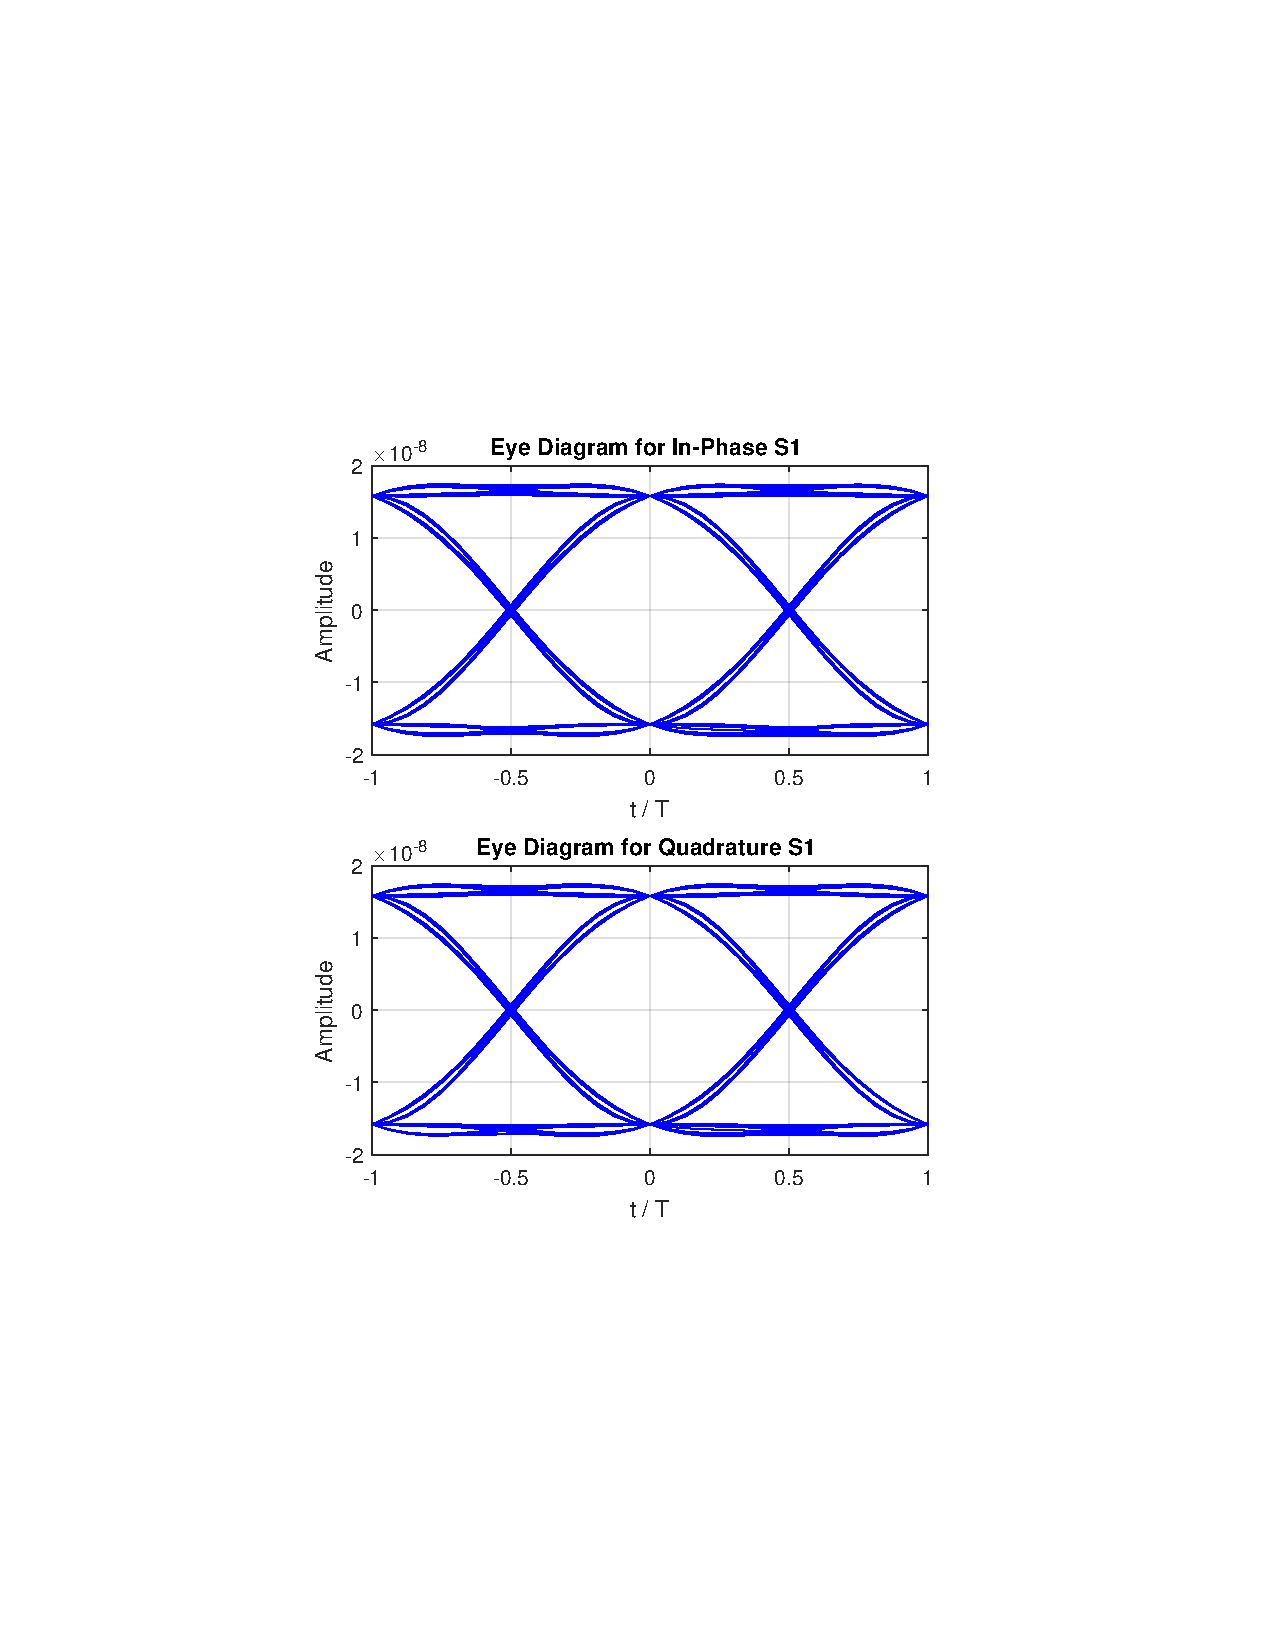
\includegraphics[clip, trim=5cm 7cm 5cm 7cm,
			width=\textwidth]{./sdf/m_qam_system/figures/eye120db09ro.pdf}
	\end{subfigure}%
	\begin{subfigure}{.5\textwidth}
		\centering
		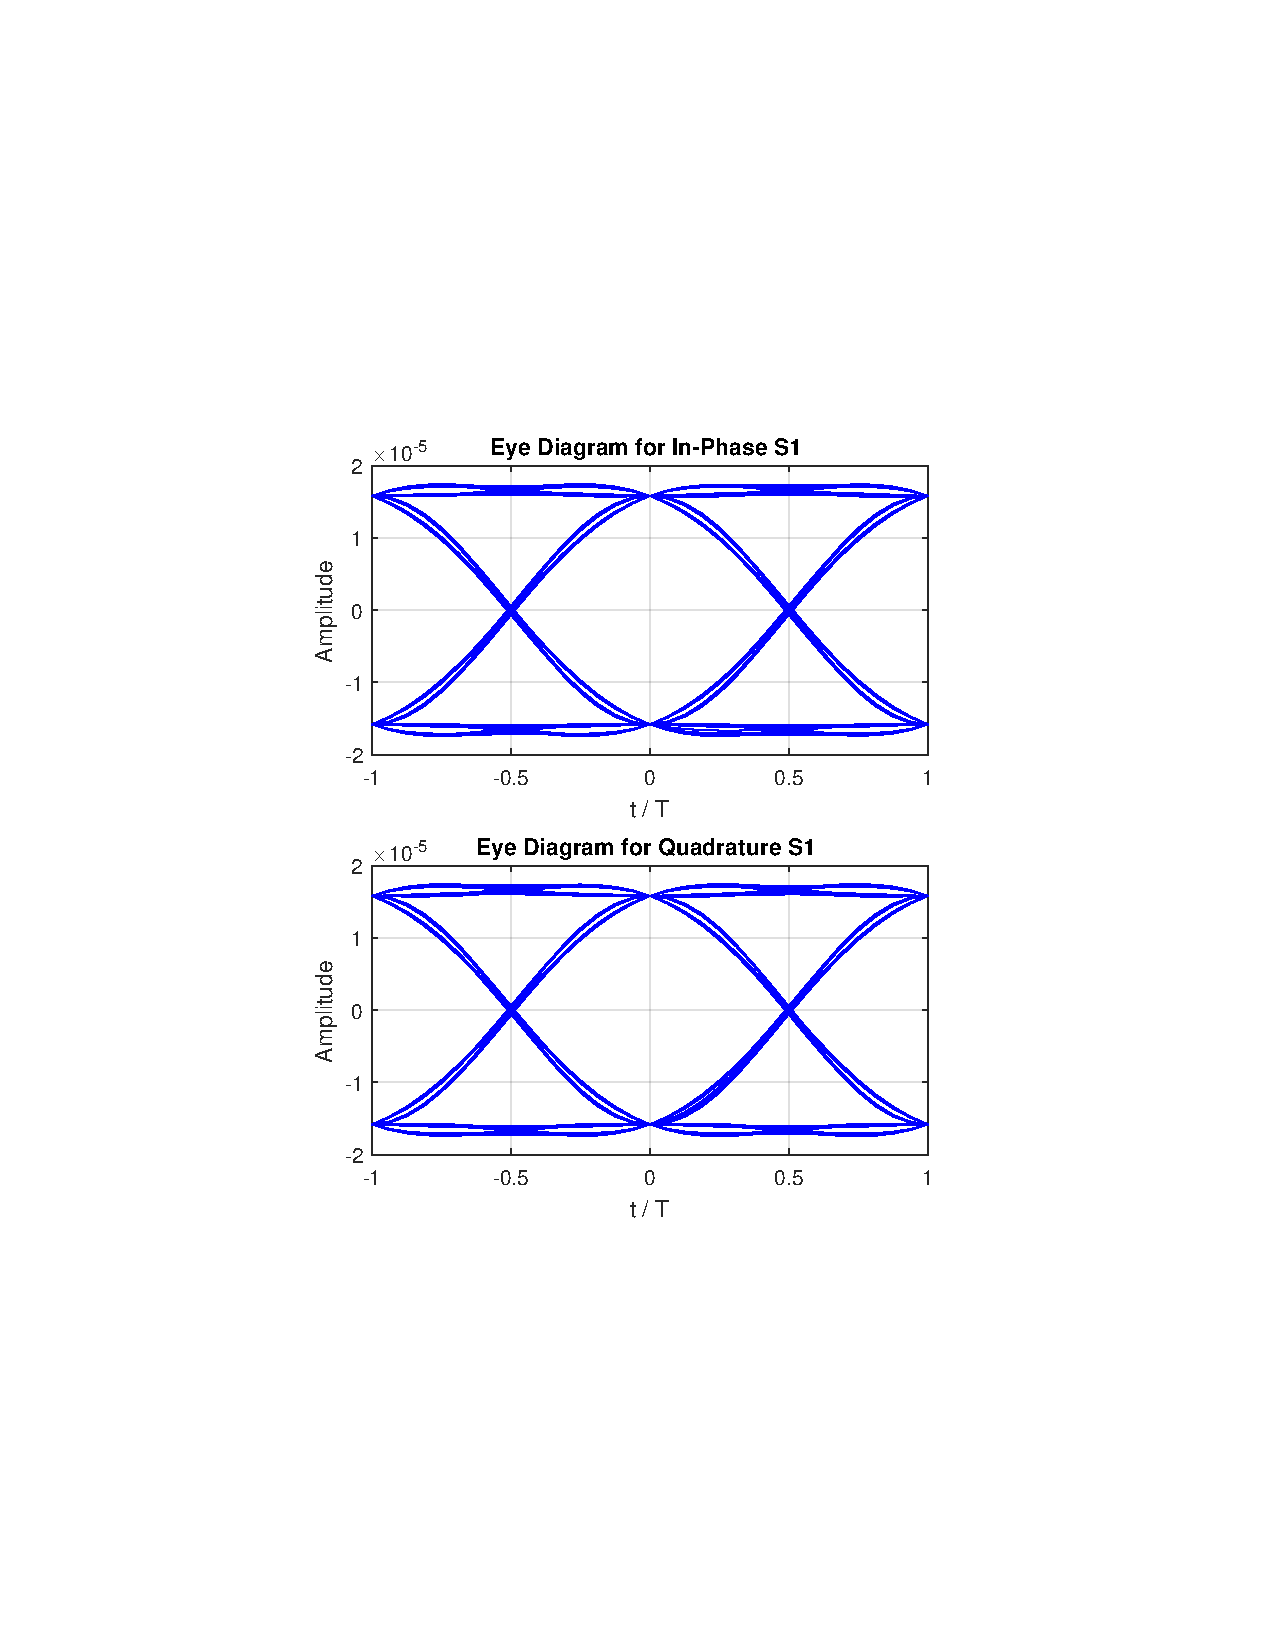
\includegraphics[clip, trim=5cm 7cm 5cm 7cm,
			width=\textwidth]{./sdf/m_qam_system/figures/eye60db09ro.pdf}
	\end{subfigure}
	\caption{Eye diagrams for the S1 bandpass signal with an output optical power
		of $-120$dBm (left) and $-60$dBm (right) with no added noise.}
	\label{fig:eyespower}
\end{figure}

As mentioned previously, using matched filters in highly beneficial, as it
allows achieving much lower error rates with the same optical power.

Figure~\ref{fig:eyes_nn_rc_09} shows the eye diagrams of the signal at the
three mentioned points, for a system without any added white noise, while using
matched filtering. The filter used in this case is a raised cosine filter with
a roll-off factor of 0.9. Although this is the ideal filter to use for pulse
shaping, as it does not cause inter-symbol-interference, it can be seen that
when used twice its results are less than ideal, as shown in the eye diagram
captured after the second filter.

\begin{figure}[H]
	\centering
	\begin{subfigure}{.45\textwidth}
		\centering
		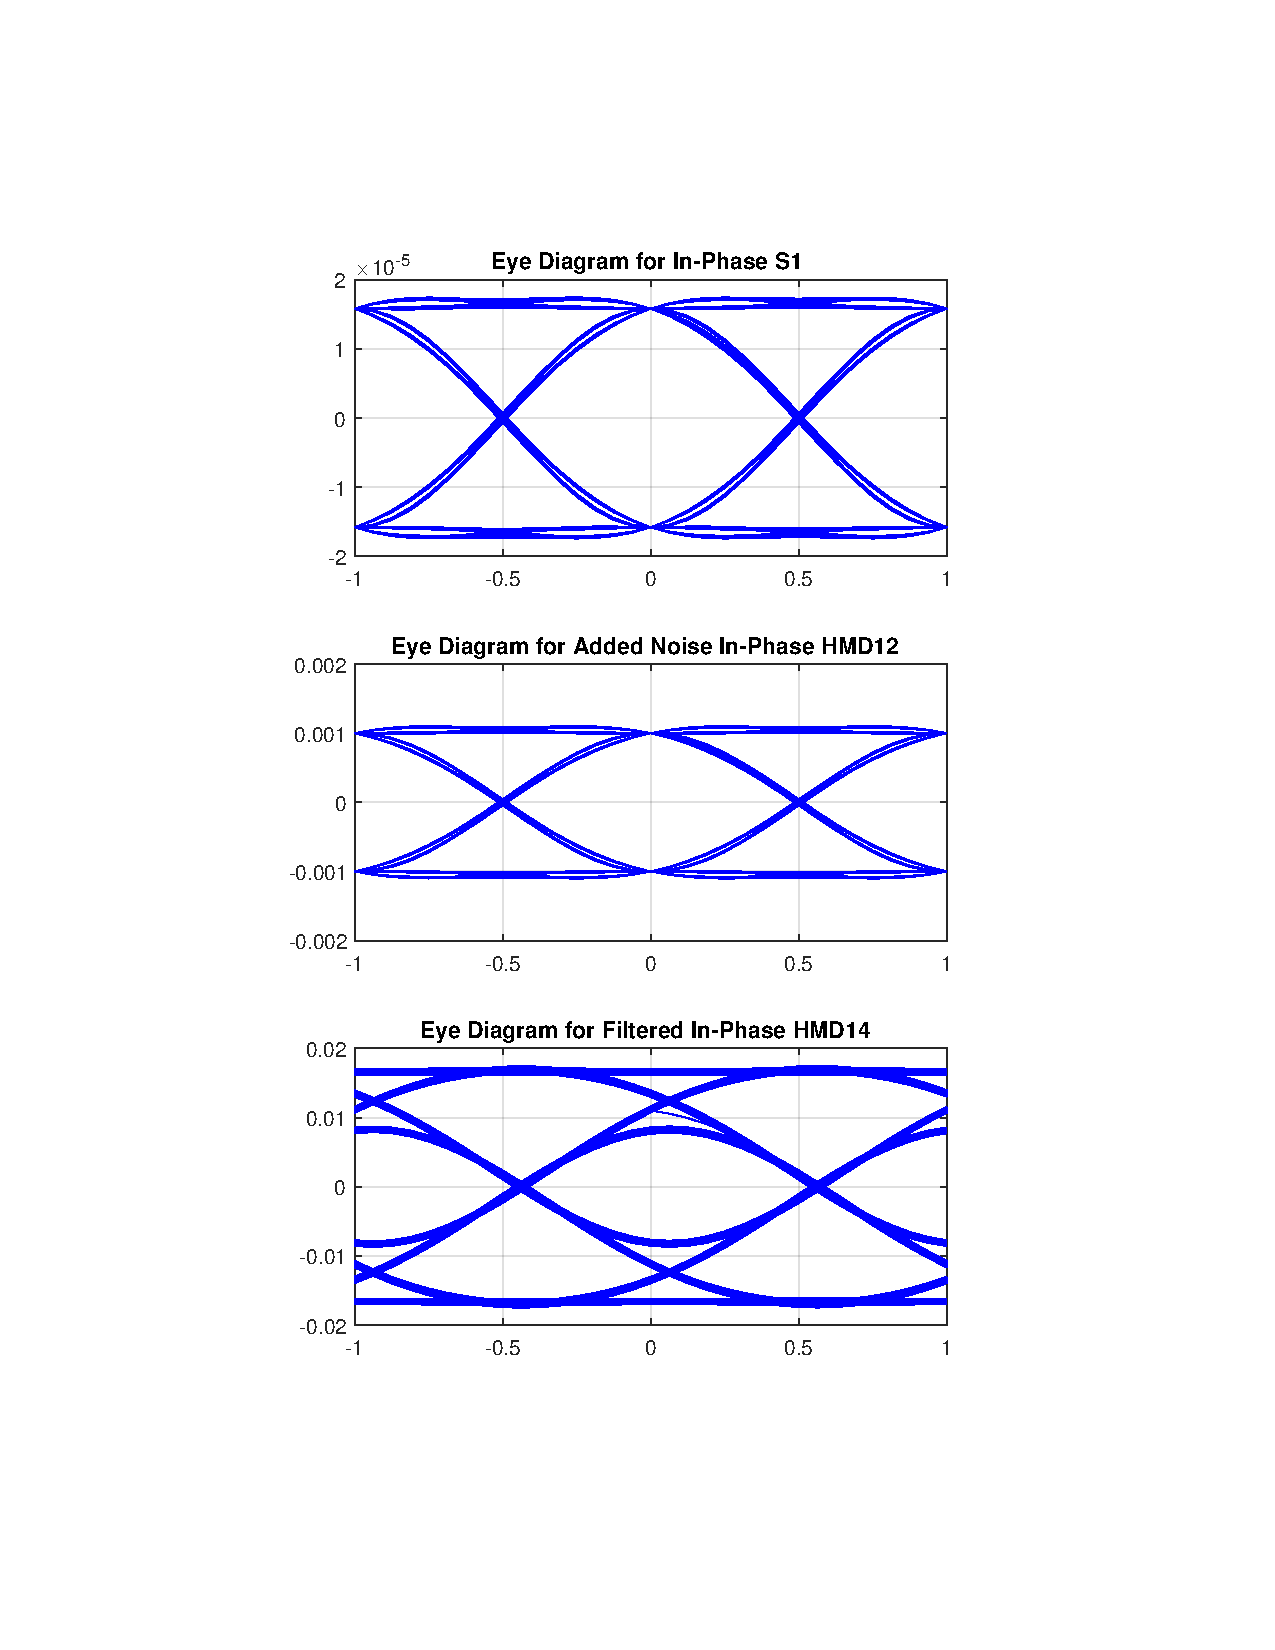
\includegraphics[clip, trim=5cm 4cm 5cm 4cm,
			width=\textwidth]{./sdf/m_qam_system/figures/eyes/if_nn_p_60_09_rc.pdf}
	\end{subfigure}
	\begin{subfigure}{.45\textwidth}
		\centering
		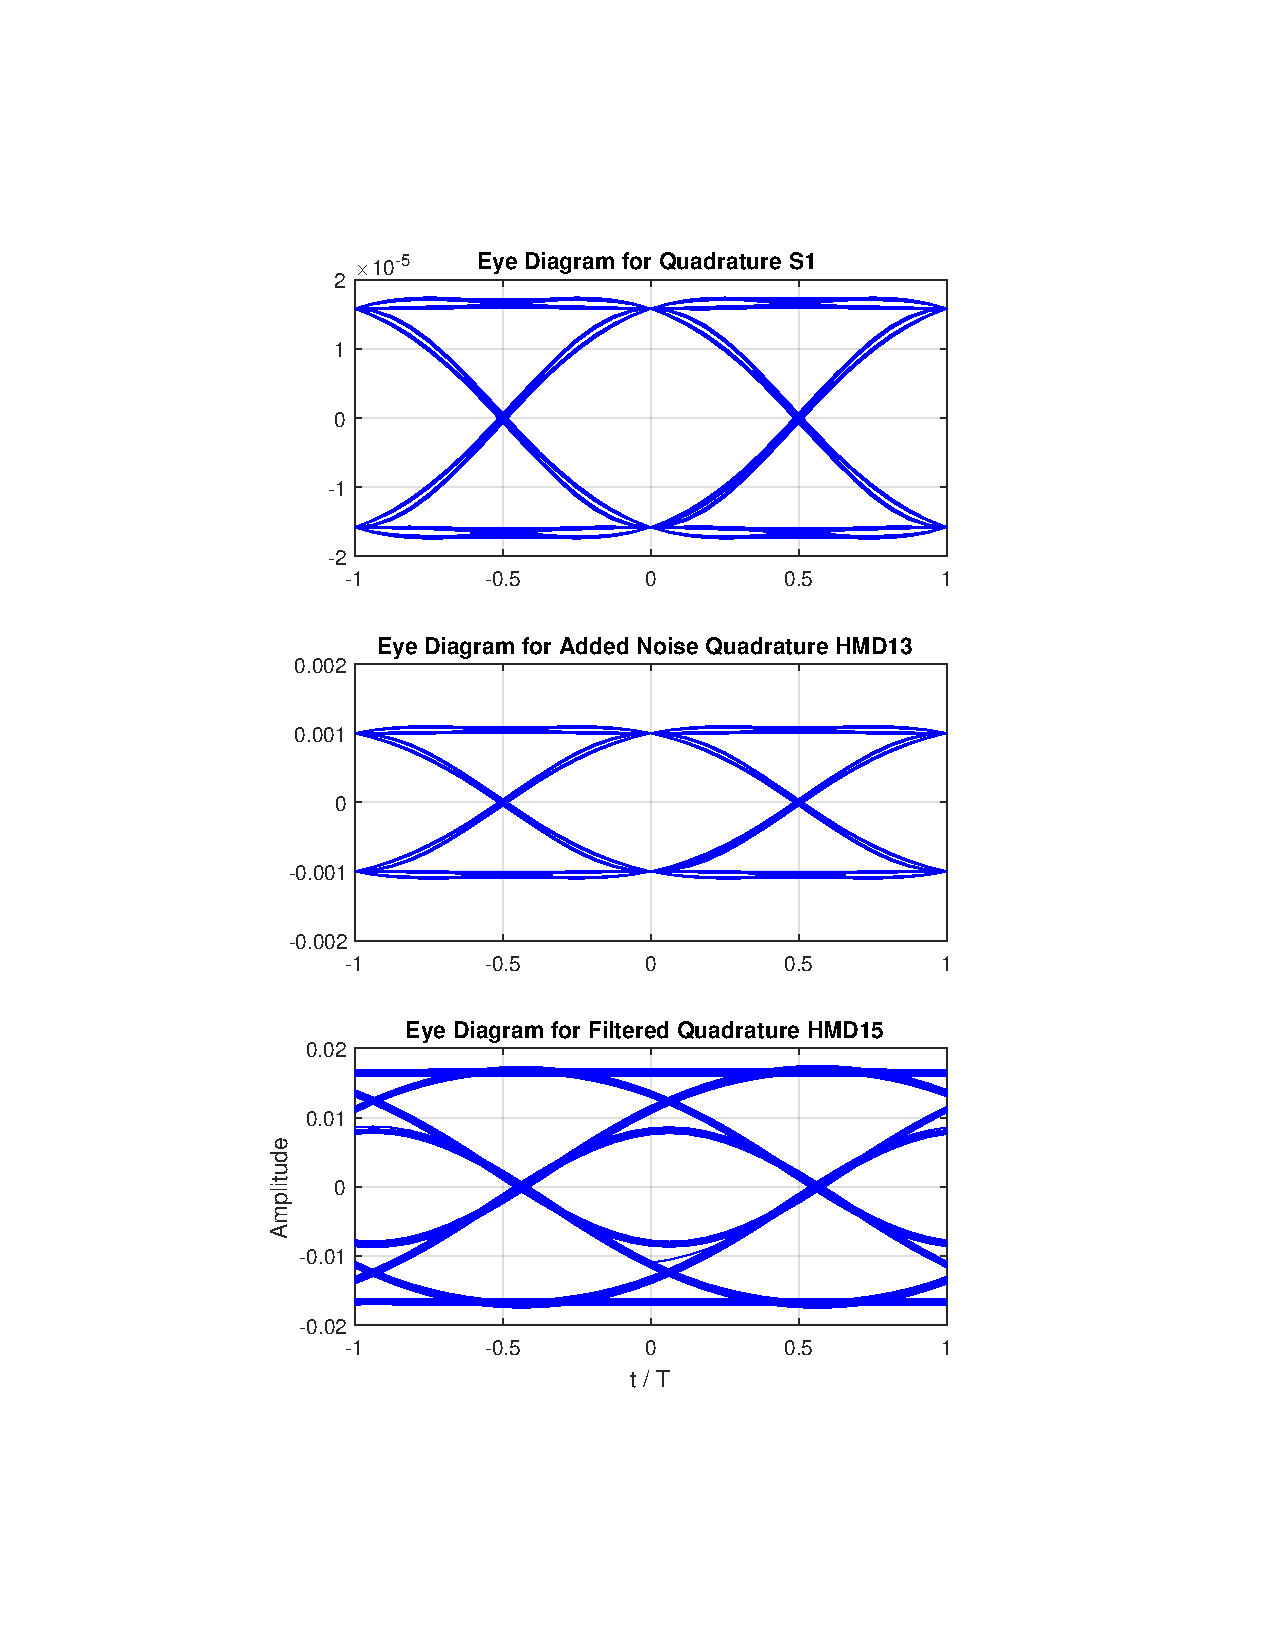
\includegraphics[clip, trim=5cm 4cm 5cm 4cm,
			width=\textwidth]{./sdf/m_qam_system/figures/eyes/q_nn_p_60_09_rc.pdf}
	\end{subfigure}
	
	\caption{Eye diagrams using matched filtering with raised-cosine at
		three different points, without AWGN: the optical output signal S1 on the top;
		the amplified signal at the middle, HMD12 and HMD13 for both components; and
		after passing through the last root-raised-cosine filter, HMD14 and HMD15, for
		both components. Obtained through simulation with an optical power output of
		-60 dBm, 0 dBm at the local oscillator, a gain of $10^3$ at the amplifier, and
		a rolloff factor of 0.9.\label{fig:eyes_nn_rc_09}}
	
\end{figure}

The optimum solution to achieving no inter-symbol interference while using
matched filtering is to use a root-raised-cosine to do the pulse-shaping at the
transmitter and the filtering at the receiver. The corresponding output of
applying twice a root-raised-cosine is exactly the same as using a
raised-cosine once. As such, the end result suffers from no inter-symbol
interference while reaping the benefits of optimum matched filtering.
Figure~\ref{fig:eyes_nn_rrc_09} shows the eye diagrams when using
root-raised-cosine filter both in the transmitter's pulse-shaper and at the
receiver's filter. The roll-off factor used in both was 0.9. It can be seen
that the shape of the eye diagram is equal to that of
Figure~\ref{fig:eyespower}, which uses a single raised cosine filter at the
pulse-shaper. Thus, it shows no sign of inter-symbol interference.

\begin{figure}[H]
	\centering
	\begin{subfigure}{.45\textwidth}
		\centering
		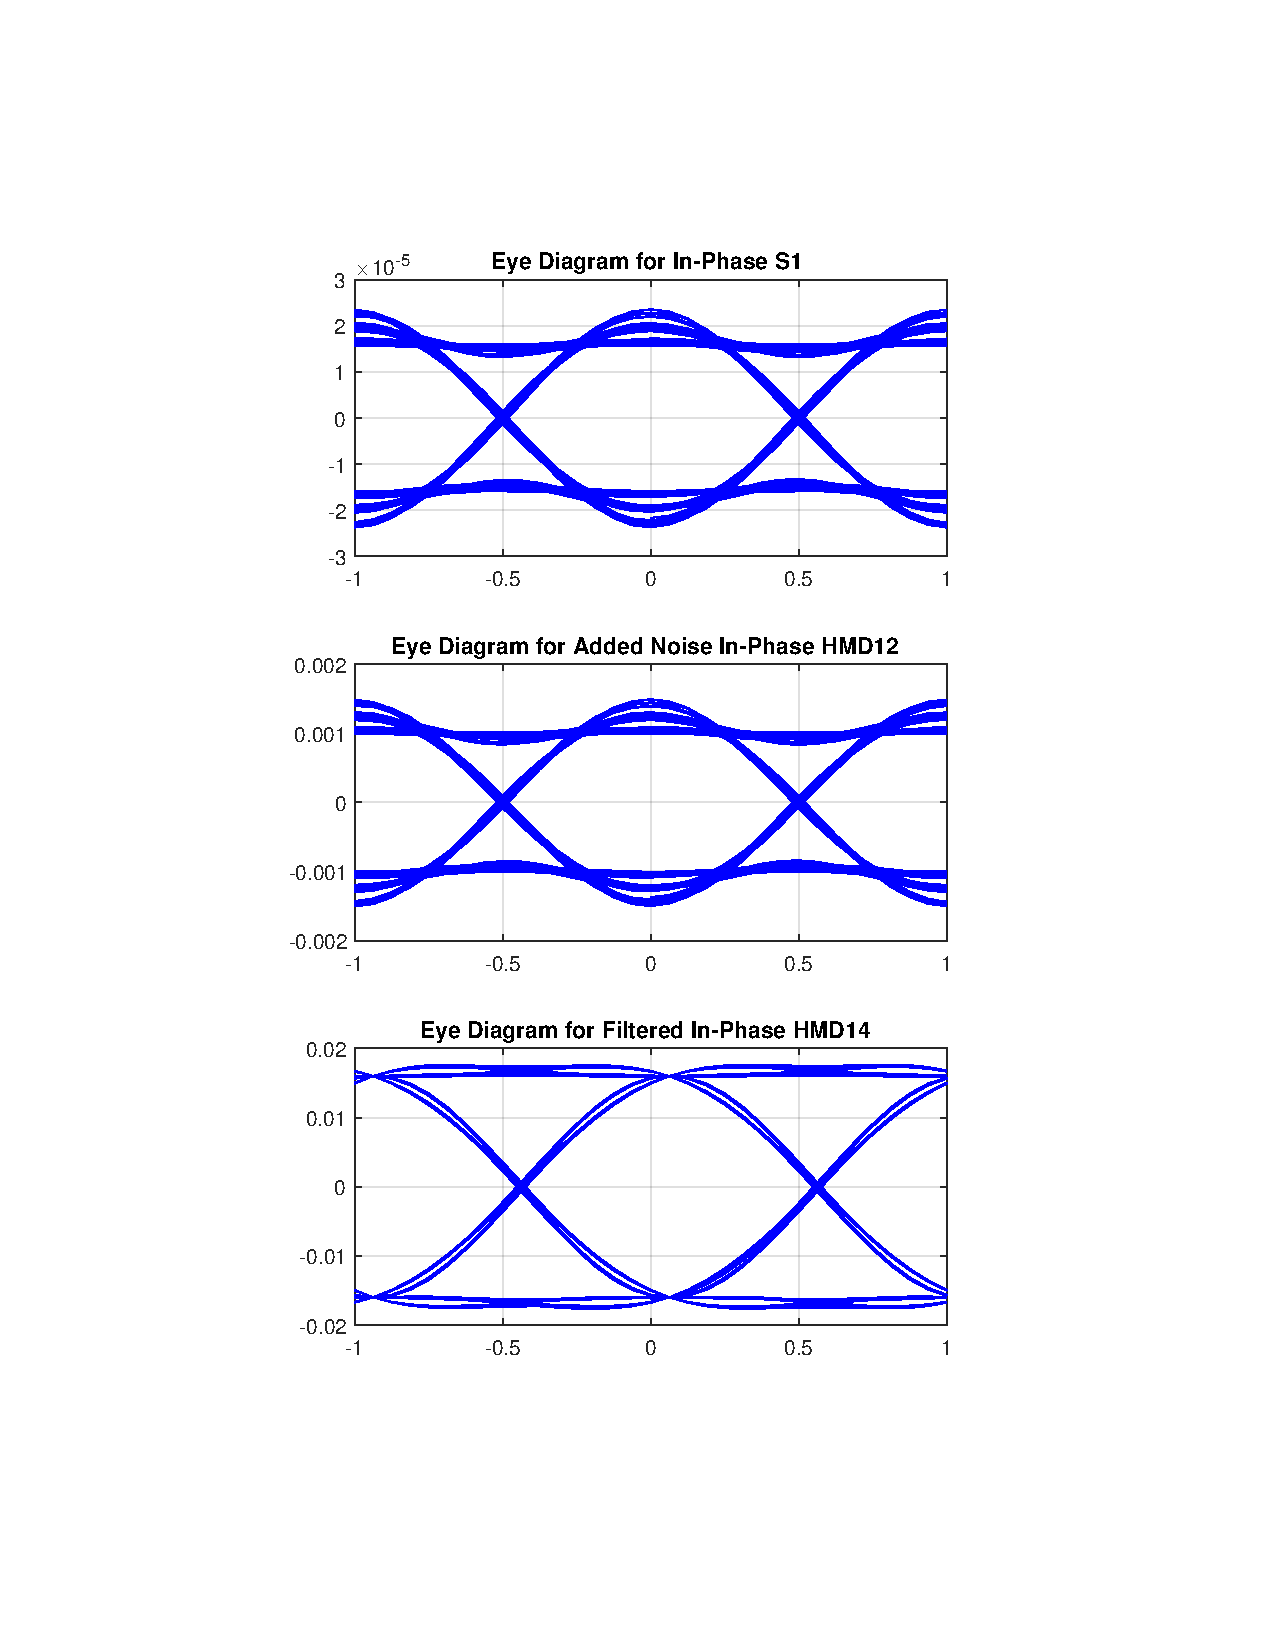
\includegraphics[clip, trim=5cm 4cm 5cm 4cm,
			width=\textwidth]{./sdf/m_qam_system/figures/eyes/if_nn_p_60_09.pdf}
	\end{subfigure}
	\begin{subfigure}{.45\textwidth}
		\centering
		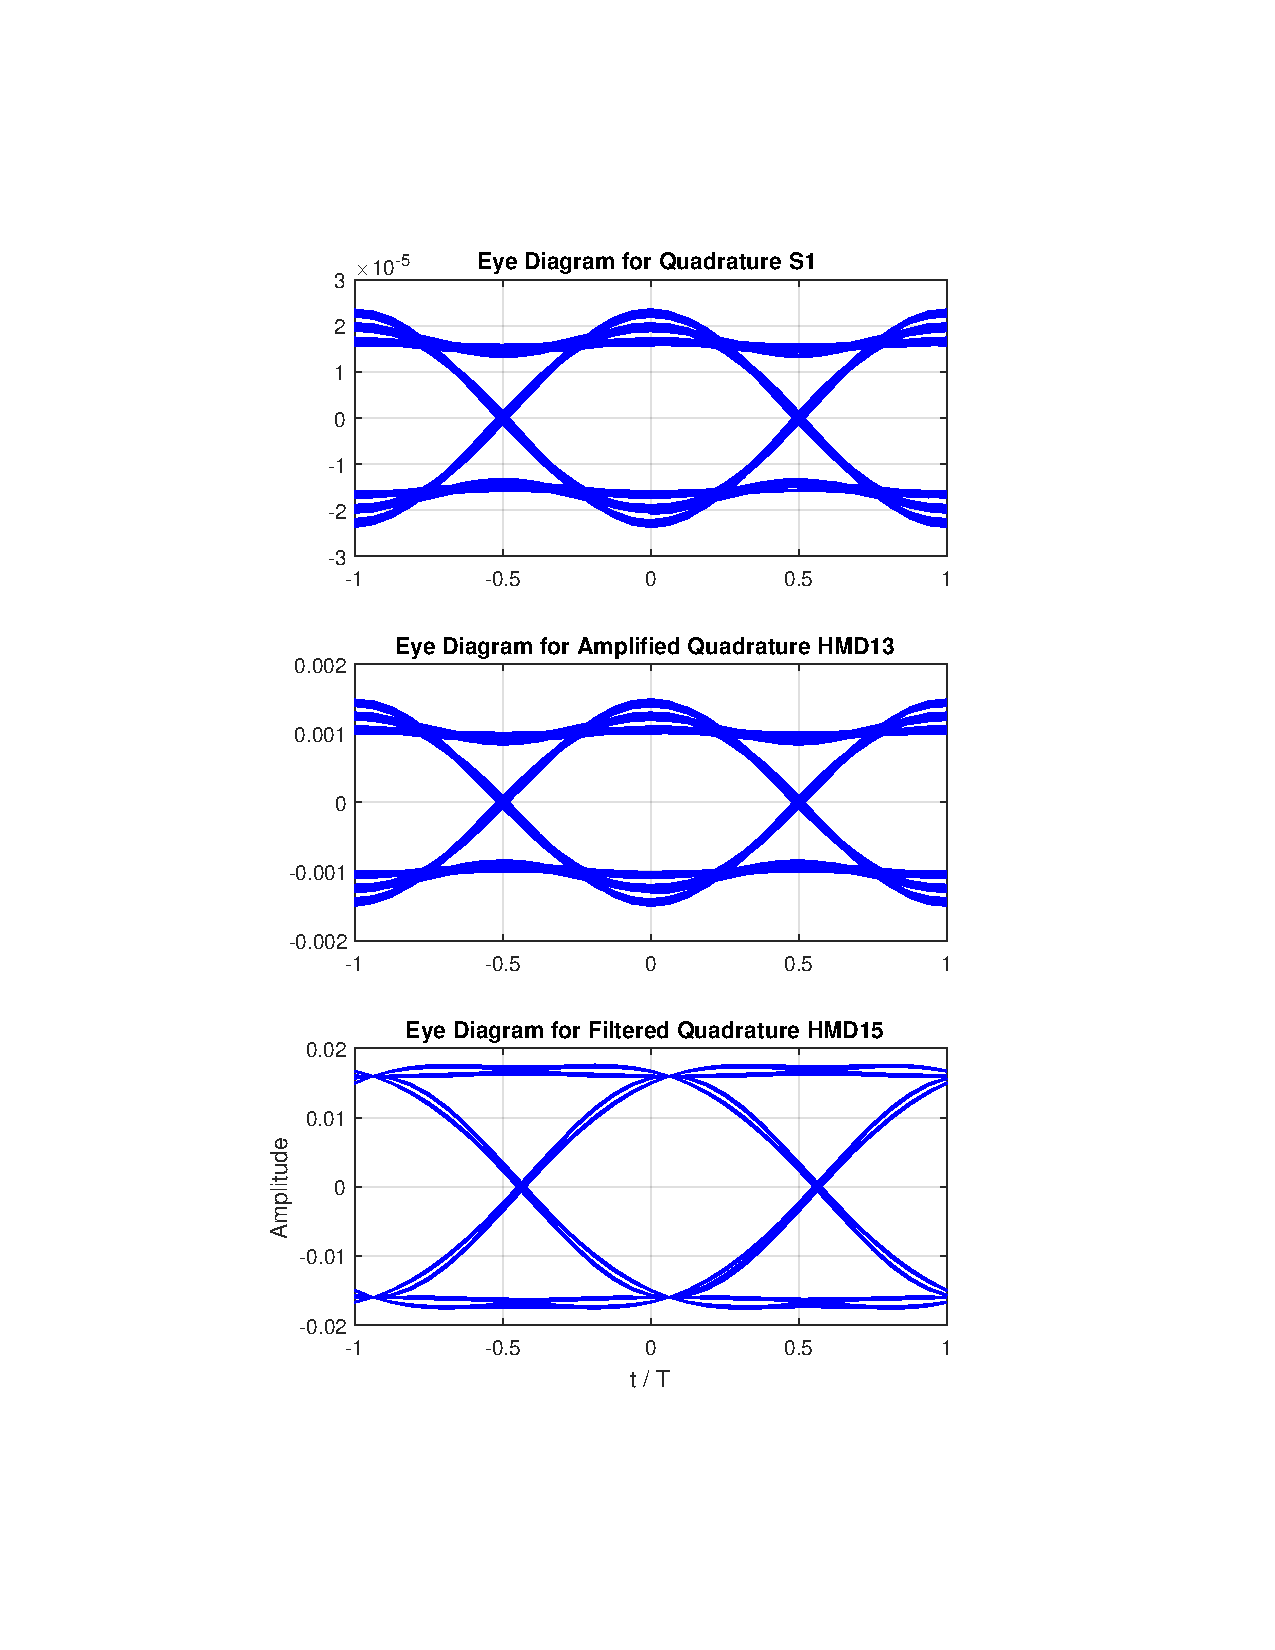
\includegraphics[clip, trim=5cm 4cm 5cm 4cm,
			width=\textwidth]{./sdf/m_qam_system/figures/eyes/q_nn_p_60_09.pdf}
	\end{subfigure}
	\caption{Eye diagrams using matched filtering with root-raised-cosine
		at three different points, without AWGN: the optical output signal S1 on the
		top; the amplified signal at the middle, HMD12 and HMD13 for both components;
		and after passing through the last root-raised-cosine filter, HMD14 and HMD15,
		for both components. Obtained through simulation with an optical power output
		of -60 dBm, 0 dBm at the local oscillator, a gain of $10^3$ at the amplifier,
		and a rolloff factor of 0.9.\label{fig:eyes_nn_rrc_09}}
	
\end{figure}

Figures~\ref{fig:eyes_nn_rrc_03} and~\ref{fig:eyes_nn_rrc_03} show a similar
comparison between matched filtering using raised-cosine or root-raised-cosine
filters, but with a roll-off factor of 0.3. Again, it can be seen that the
final shape of the eye diagram when using the root-raised-cosine for matched
filtering is the same as the shape of the optical signal S1 when using a
raised-cosine-filter.

\begin{figure}[H]
	\centering
	\begin{subfigure}{.45\textwidth}
		\centering
		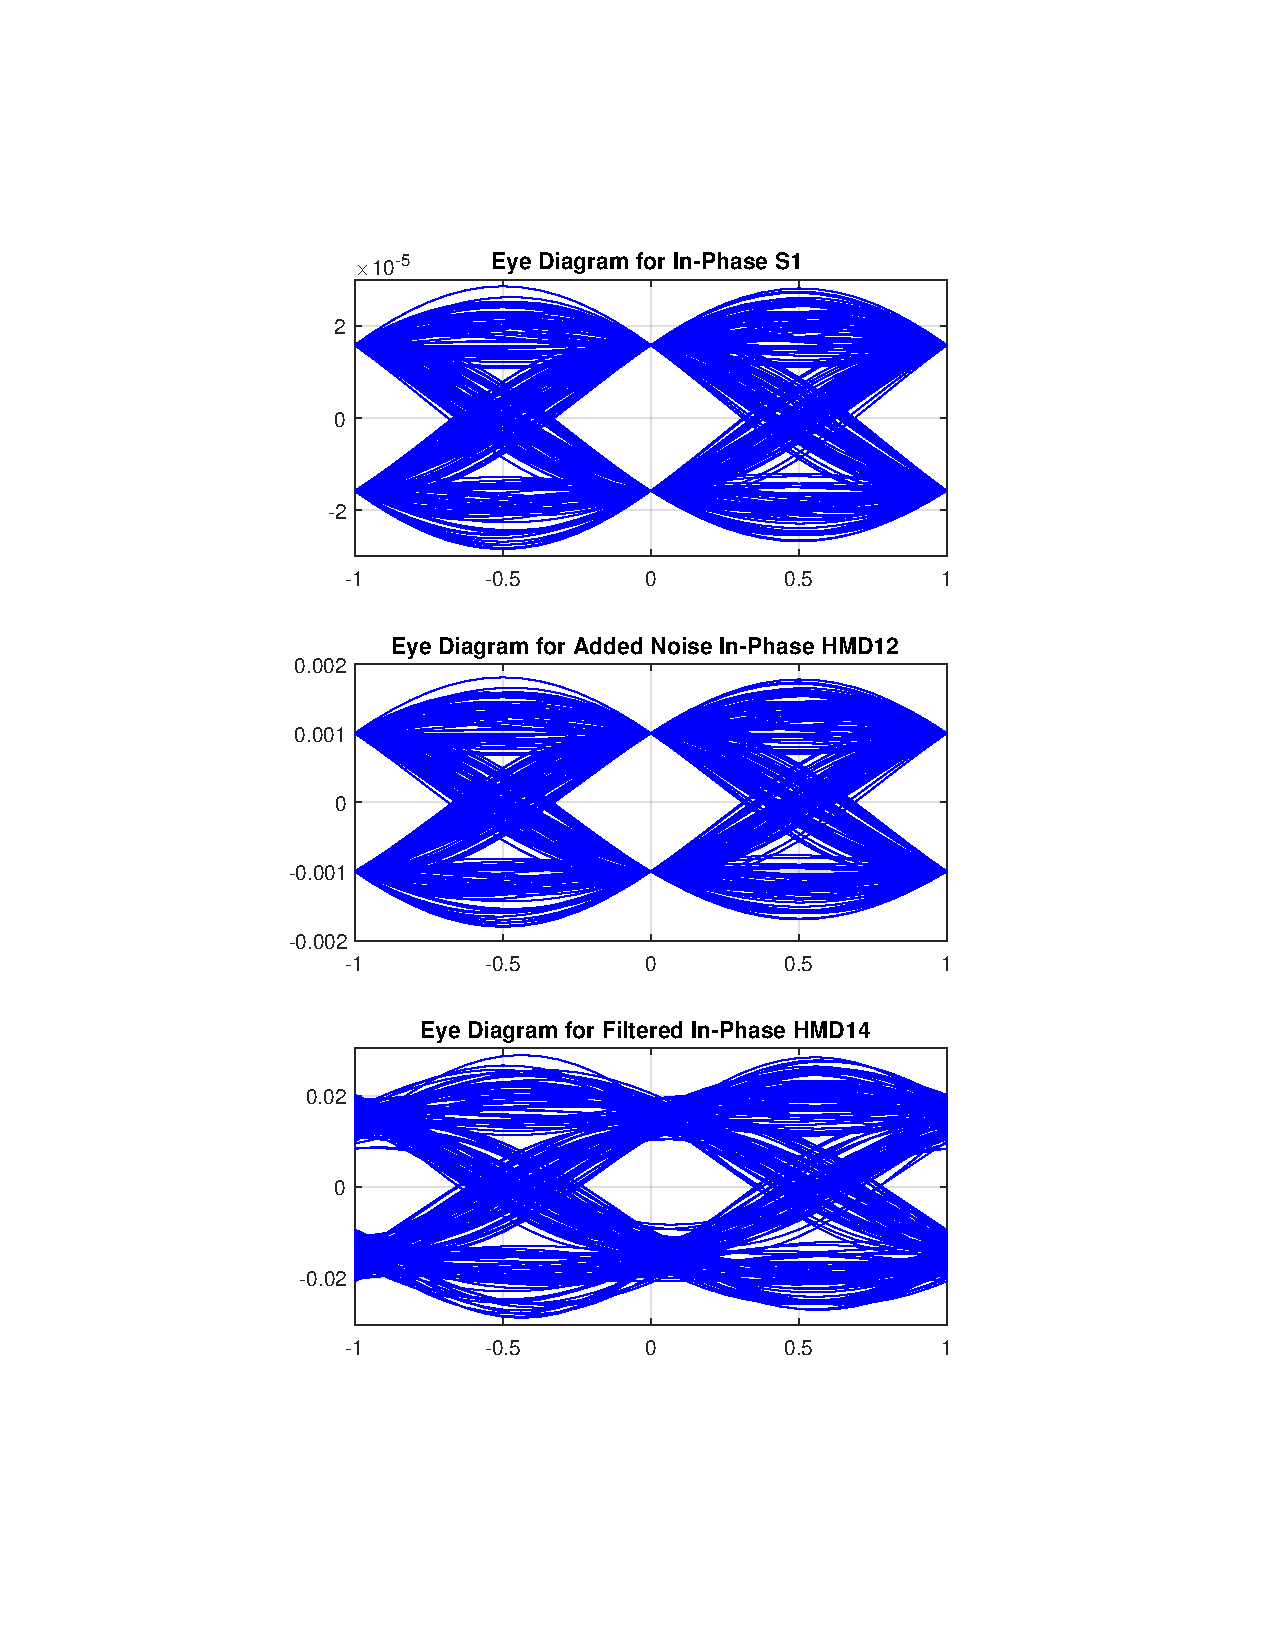
\includegraphics[clip, trim=5cm 4cm 5cm 4cm,
			width=\textwidth]{./sdf/m_qam_system/figures/eyes/if_nn_p_60_03_rc.pdf}
	\end{subfigure}
	\begin{subfigure}{.45\textwidth}
		\centering
		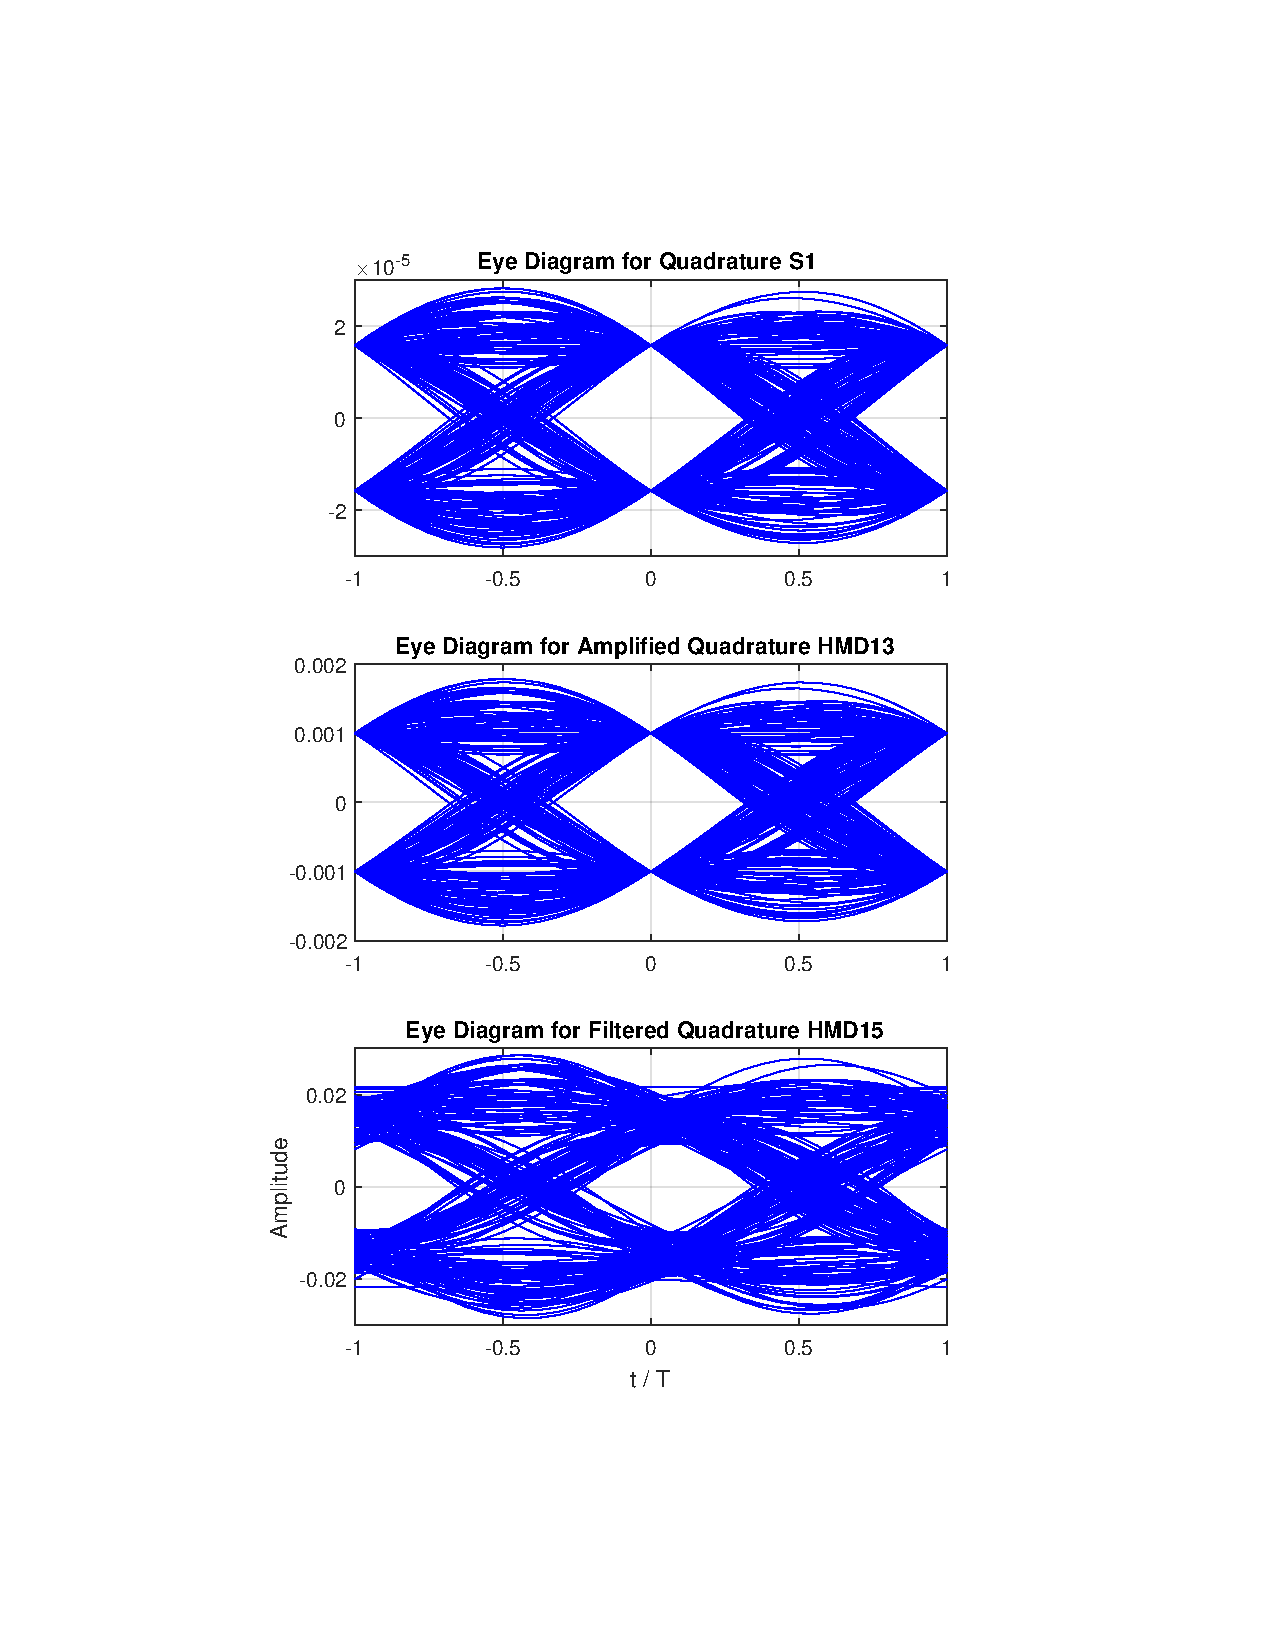
\includegraphics[clip, trim=5cm 4cm 5cm 4cm,
			width=\textwidth]{./sdf/m_qam_system/figures/eyes/q_nn_p_60_03_rc.pdf}
	\end{subfigure}
	
	\caption{Eye diagrams using matched filtering with raised-cosine at
		three different points, without AWGN: the optical output signal S1 on the top;
		the amplified signal at the middle, HMD12 and HMD13 for both components; and
		after passing through the last root-raised-cosine filter, HMD14 and HMD15, for
		both components. Obtained through simulation with an optical power output of
		-60 dBm, 0 dBm at the local oscillator, a gain of $10^3$ at the amplifier, and
		a rolloff factor of 0.3.\label{fig:eyes_nn_rc_03}}
	
\end{figure}


\begin{figure}[H]
	\centering
	\begin{subfigure}{.45\textwidth}
		\centering
		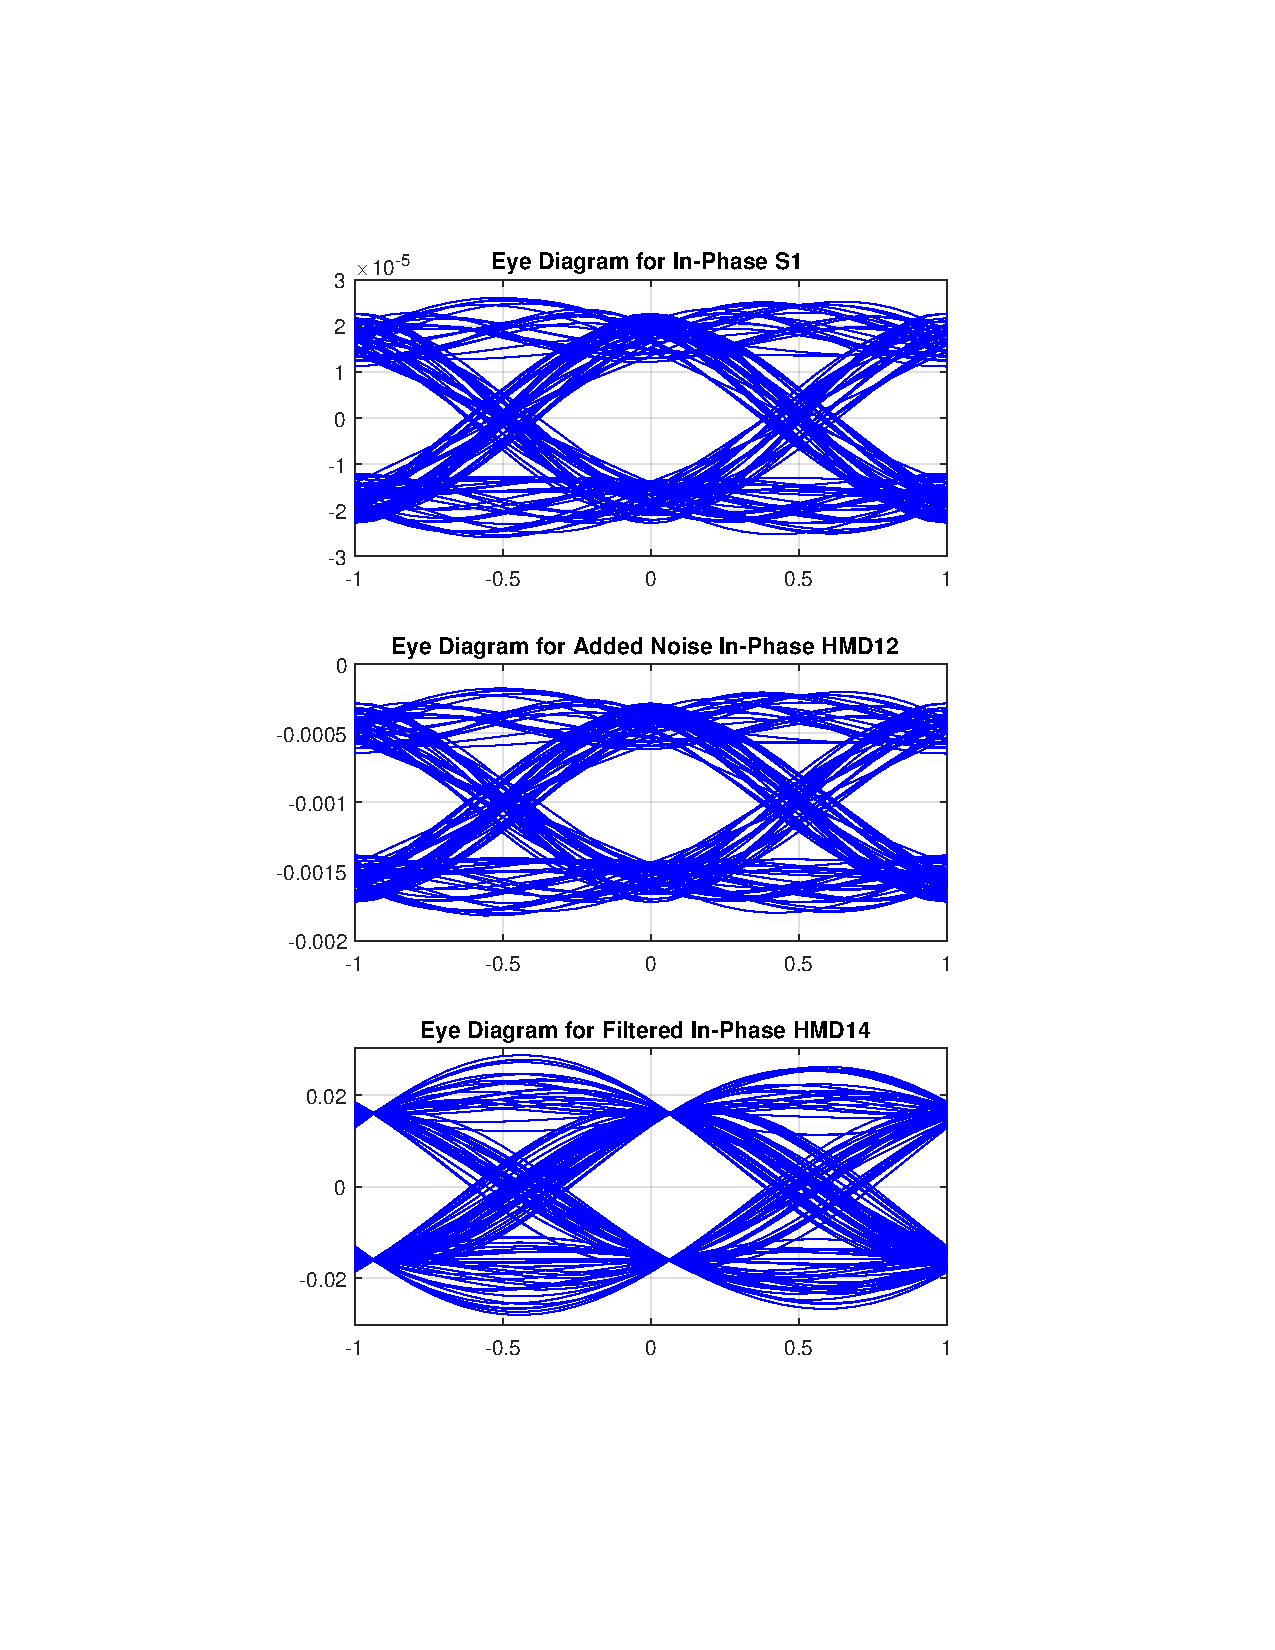
\includegraphics[clip, trim=5cm 4cm 5cm 4cm,
			width=\textwidth]{./sdf/m_qam_system/figures/eyes/if_nn_p_60_03.pdf}
	\end{subfigure}
	\begin{subfigure}{.45\textwidth}
		\centering
		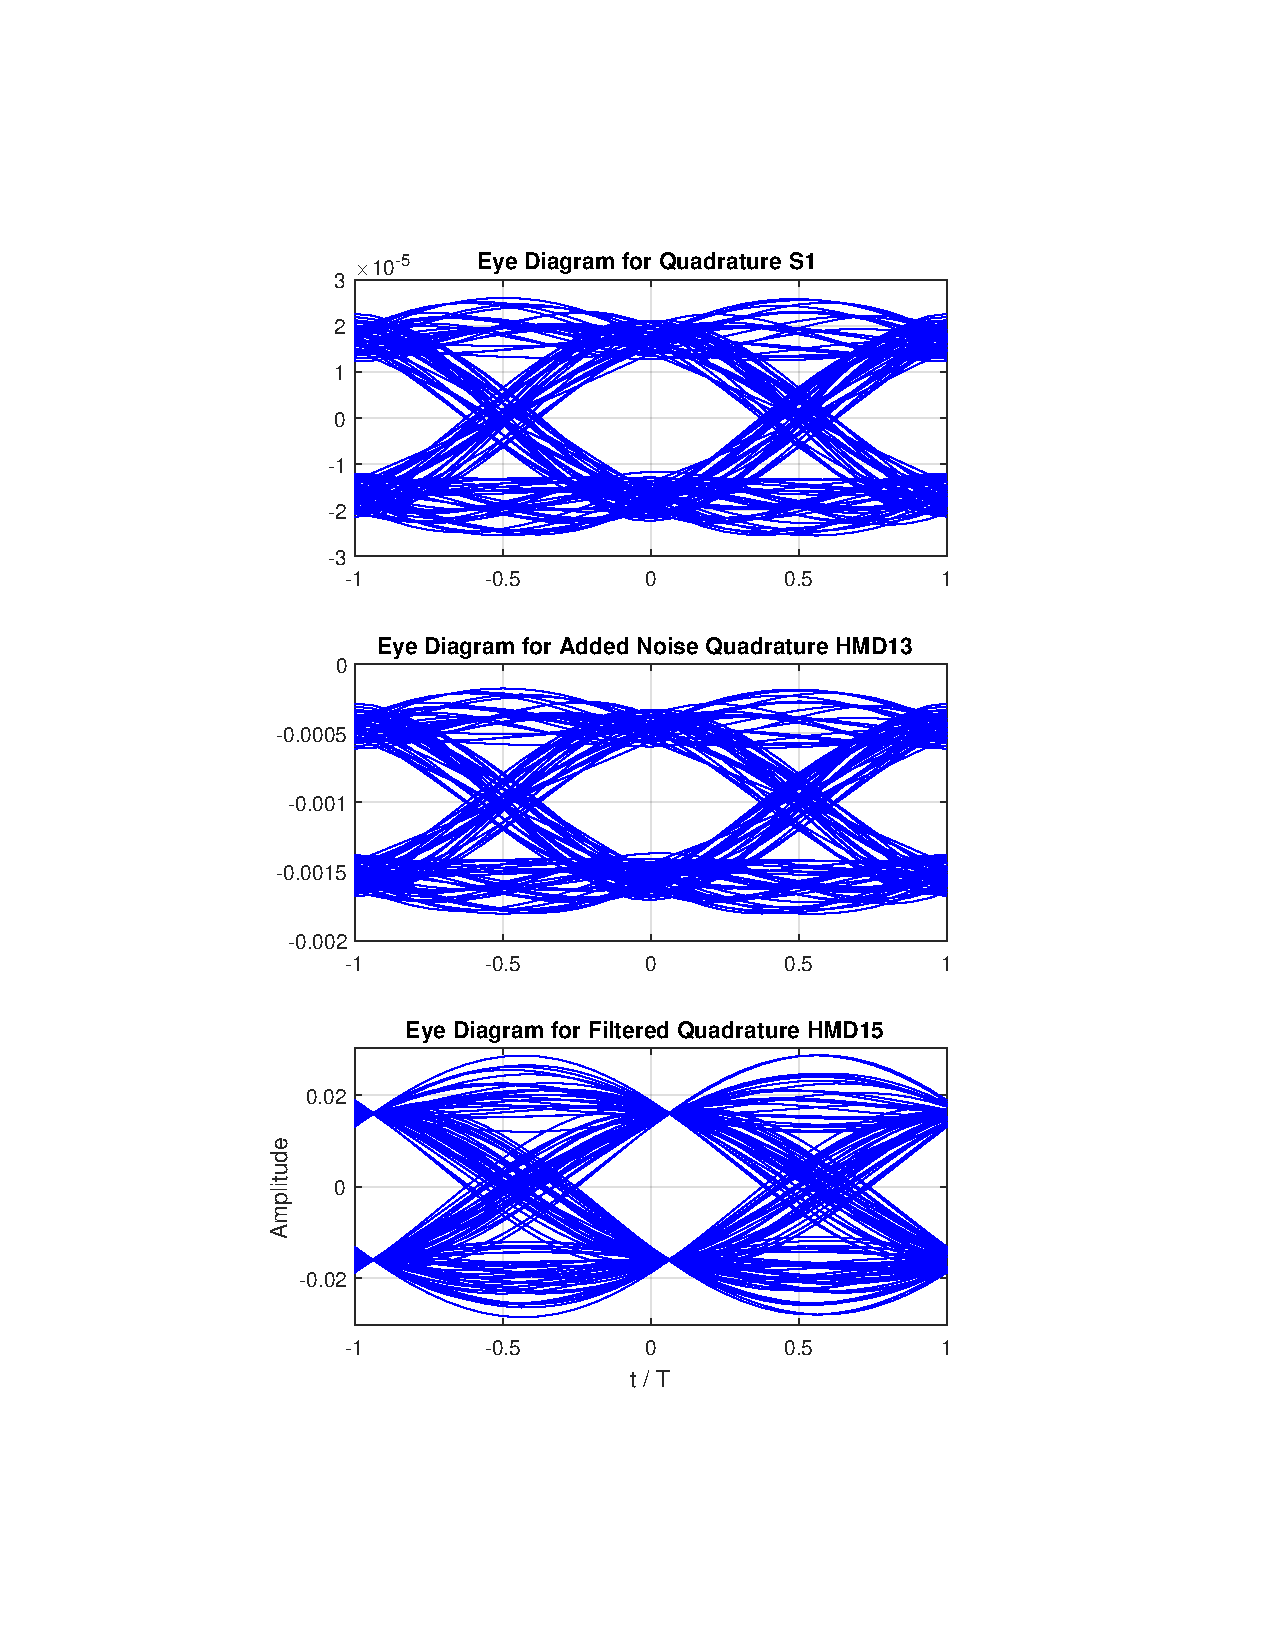
\includegraphics[clip, trim=5cm 4cm 5cm 4cm,
			width=\textwidth]{./sdf/m_qam_system/figures/eyes/q_nn_p_60_03.pdf}
	\end{subfigure}
	
	\caption{Eye diagrams using matched filtering with root-raised-cosine
		at three different points, without AWGN: the optical output signal S1 on the
		top; the amplified signal at the middle, HMD12 and HMD13 for both components;
		and after passing through the last root-raised-cosine filter, HMD14 and HMD15,
		for both components. Obtained through simulation with an optical power output
		of -60 dBm, 0 dBm at the local oscillator, a gain of $10^3$ at the amplifier,
		and a rolloff factor of 0.3.\label{fig:eyes_nn_rrc_03}}
	
\end{figure}

Thus, it can be concluded that, in order to avoid inter-symbol interference,
the filters used should be raised-cosine or root-raised-cosine, if not using a
filter at the receiver or if using matched filtering, respectively. As such,
from now on only these configurations will be used.

\subsubsection*{Signals with AWGN and high SNR}

In this section and the following one, a comparison will be presented between
not using a filter on the receiver and using matched filtering. This comparison
will be made for signals affected by added white gaussian noise, where the
noise is added to the signal after the amplifier stage and before the signal
passes through the filter on the receiver.

For the first case, where no filter is present at the receiver, a
raised-cosine filter will be used at the pulse shaper. For matched filtering, a
root-raised-cosine filter will be used at the pulse-shaper and the receiver.

Figures \ref{fig:eyes_n_rc_45_09}-\ref{fig:eyes_n_rrc_45_09} show the eye
diagrams for both these cases. The optical power used was $-45 dBm$, the
noise spectral density was set at $10^6 W/Hz$, and the roll-off factor was set
to $0.9$ in both cases. In both cases, its is still possible to visibly see the
approximate shape of the signal after noise is added, even without matched
filtering. However, it can be seen that the output signal in the case with
matched filtering is much less affected by noise, as the root-raised-cosine at
the receiver is rather effective at filtering the noise.


\begin{figure}[H]
	\centering
	\begin{subfigure}{.45\textwidth}
		\centering
		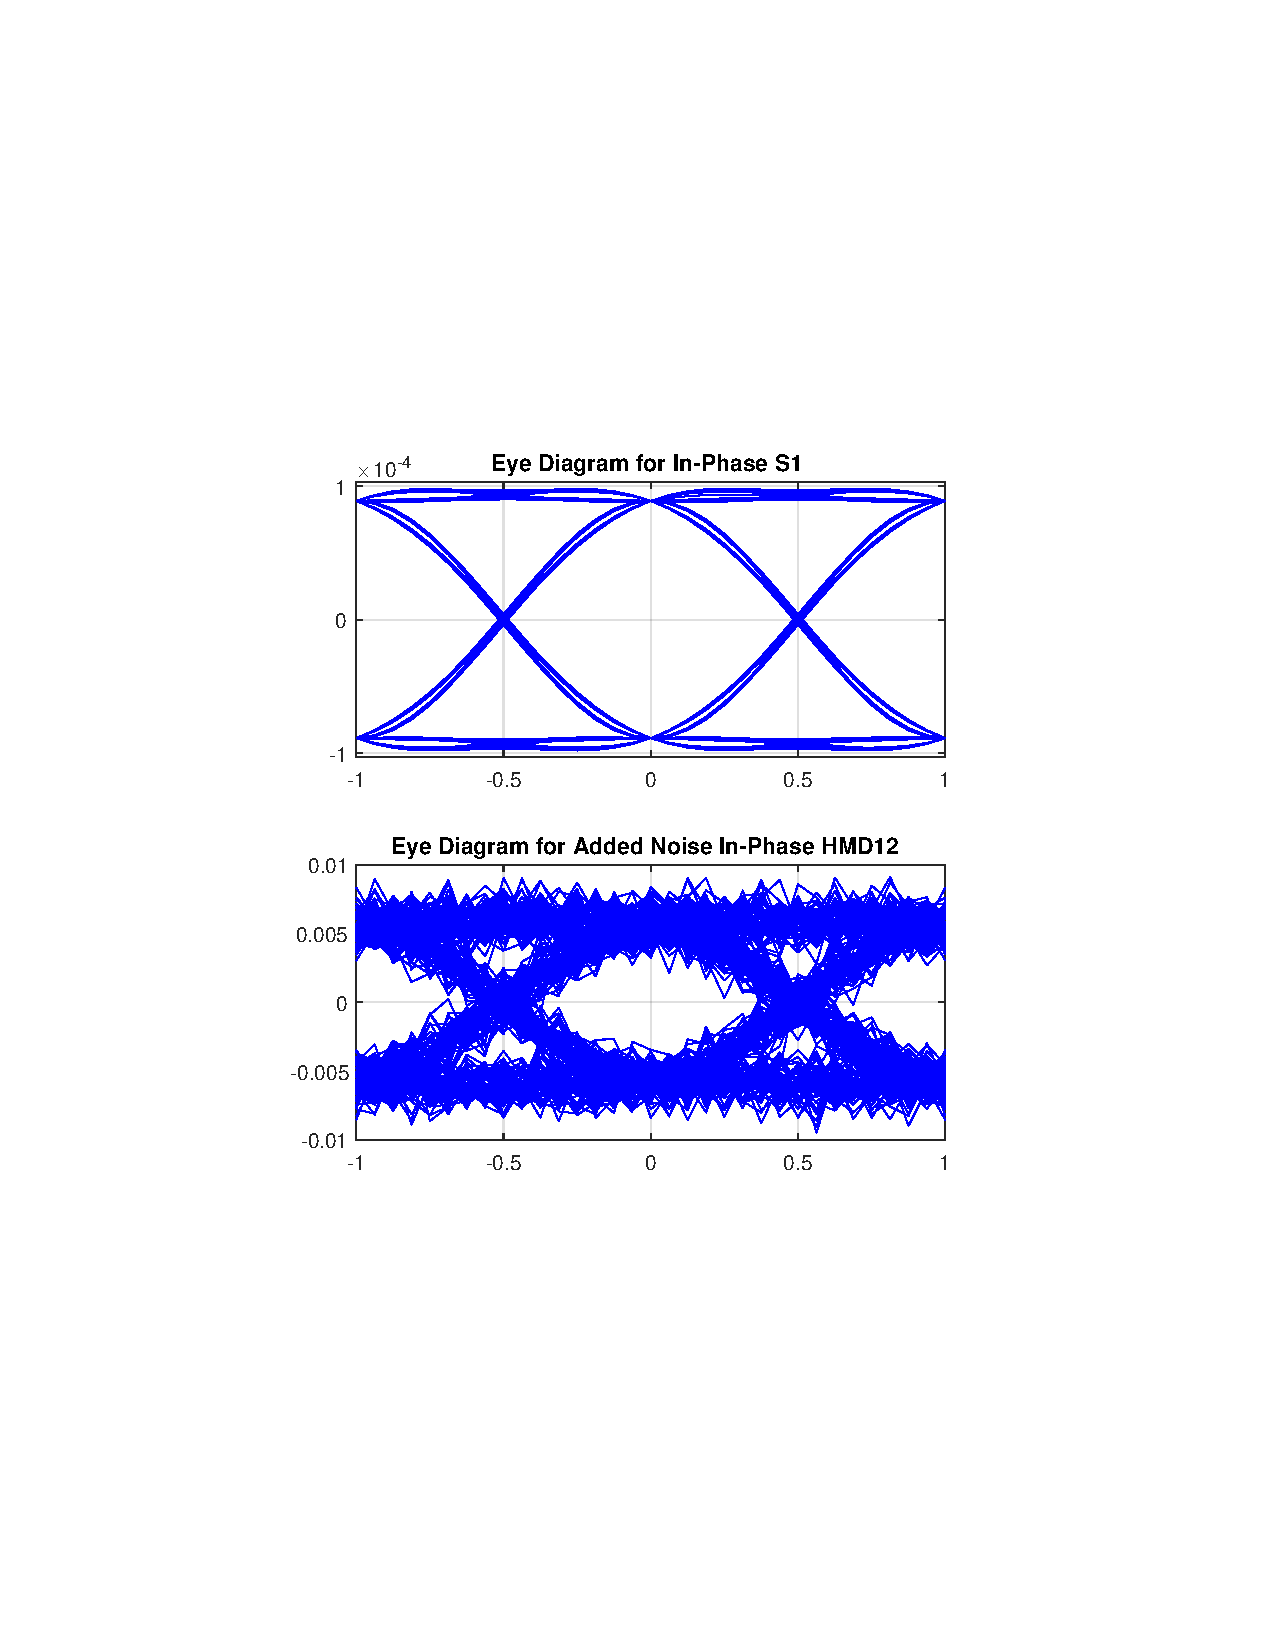
\includegraphics[clip, trim=5cm 4cm 5cm 4cm, width=\textwidth]{./sdf/m_qam_system/figures/eyes/if_n_nmf_45_60_rc_09.pdf}
	\end{subfigure}
	\begin{subfigure}{.45\textwidth}
		\centering
		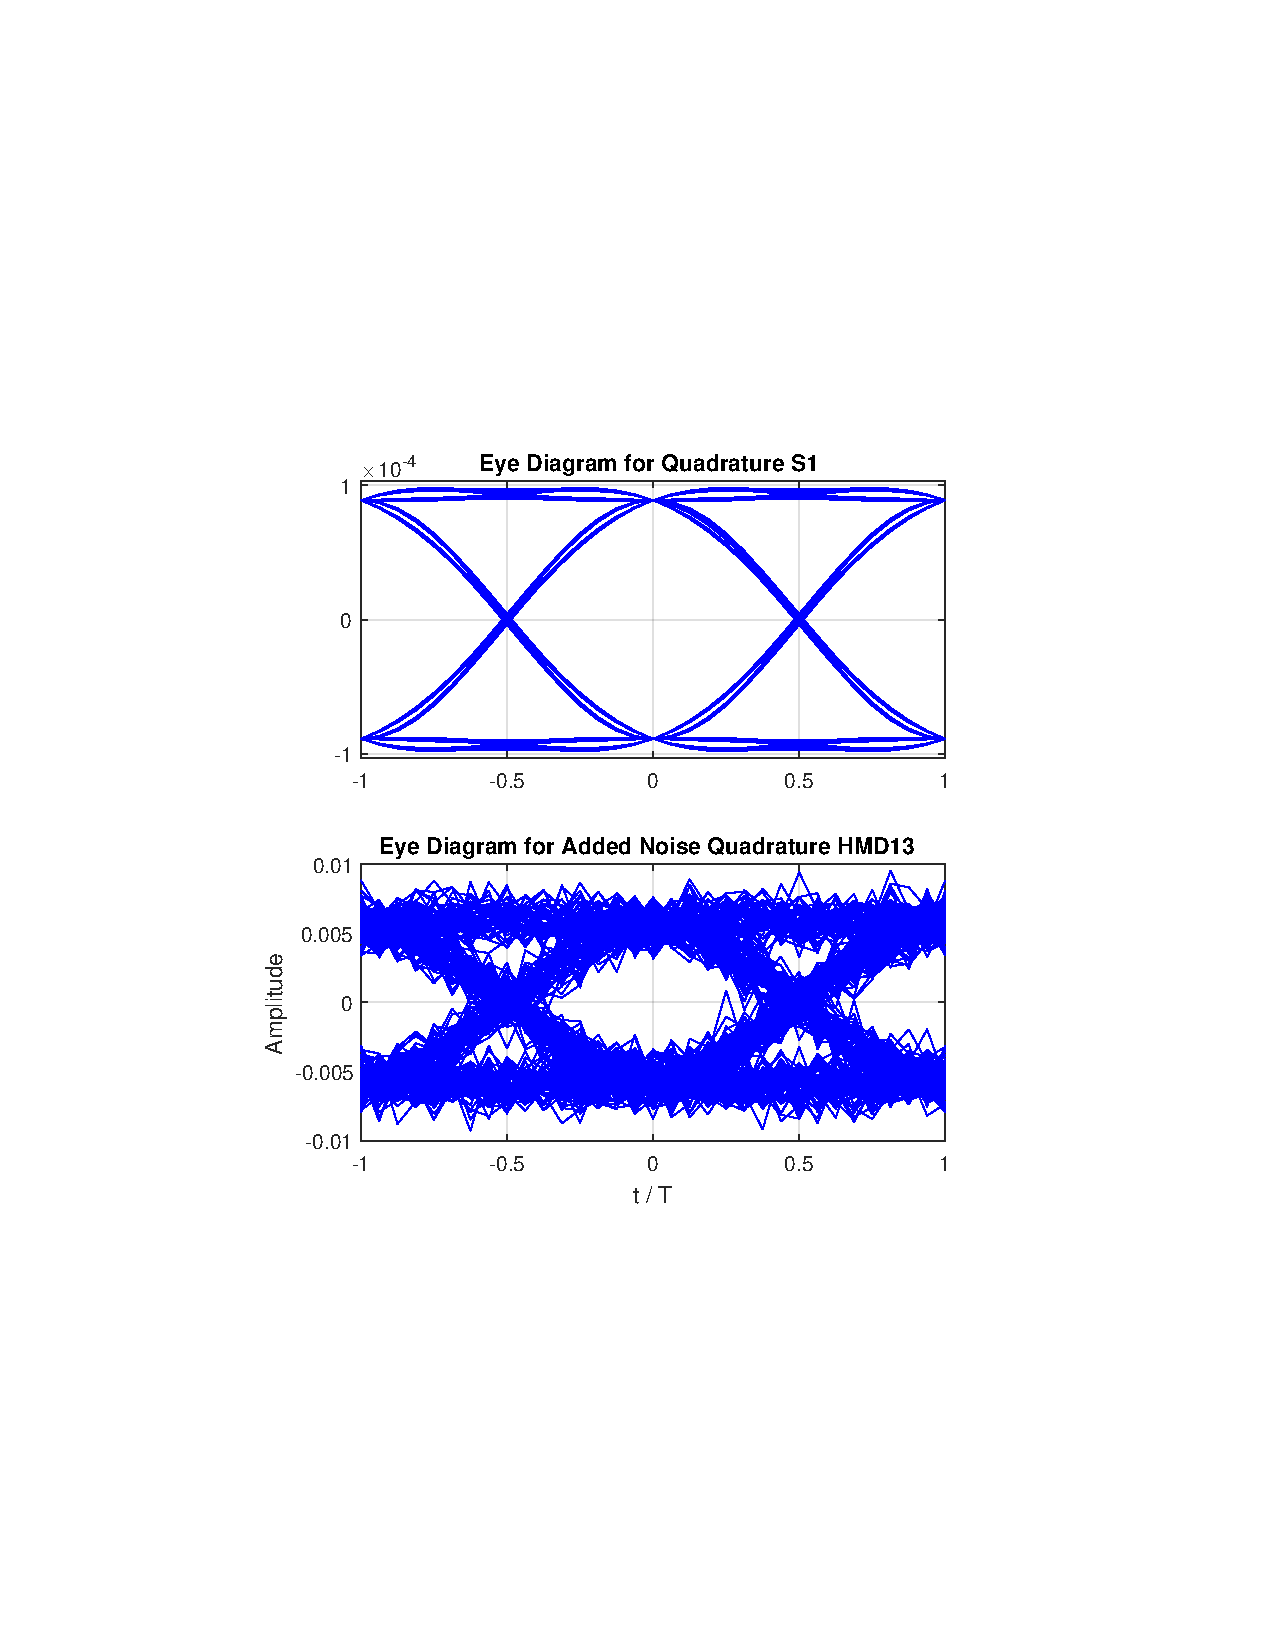
\includegraphics[clip, trim=5cm 4cm 5cm 4cm, width=\textwidth]{./sdf/m_qam_system/figures/eyes/q_n_nmf_45_60_rc_09.pdf}
	\end{subfigure}
	
	\caption{Eye diagrams without matched filtering using raised-cosine, at
		two different points: the optical output signal S1 on the top and the amplified
		signal with added noise, HMD12 and HMD13 for both components.
		Obtained through simulation with an optical power output of
		-45 dBm, 0 dBm at the local oscillator, a gain of $10^3$ at the amplifier, a
		noise spectral density of $10^{-6}$ and a rolloff factor of
		0.9.\label{fig:eyes_n_rc_45_09}}
\end{figure}

\begin{figure}[H]
	\centering
	\begin{subfigure}{.45\textwidth}
		\centering
		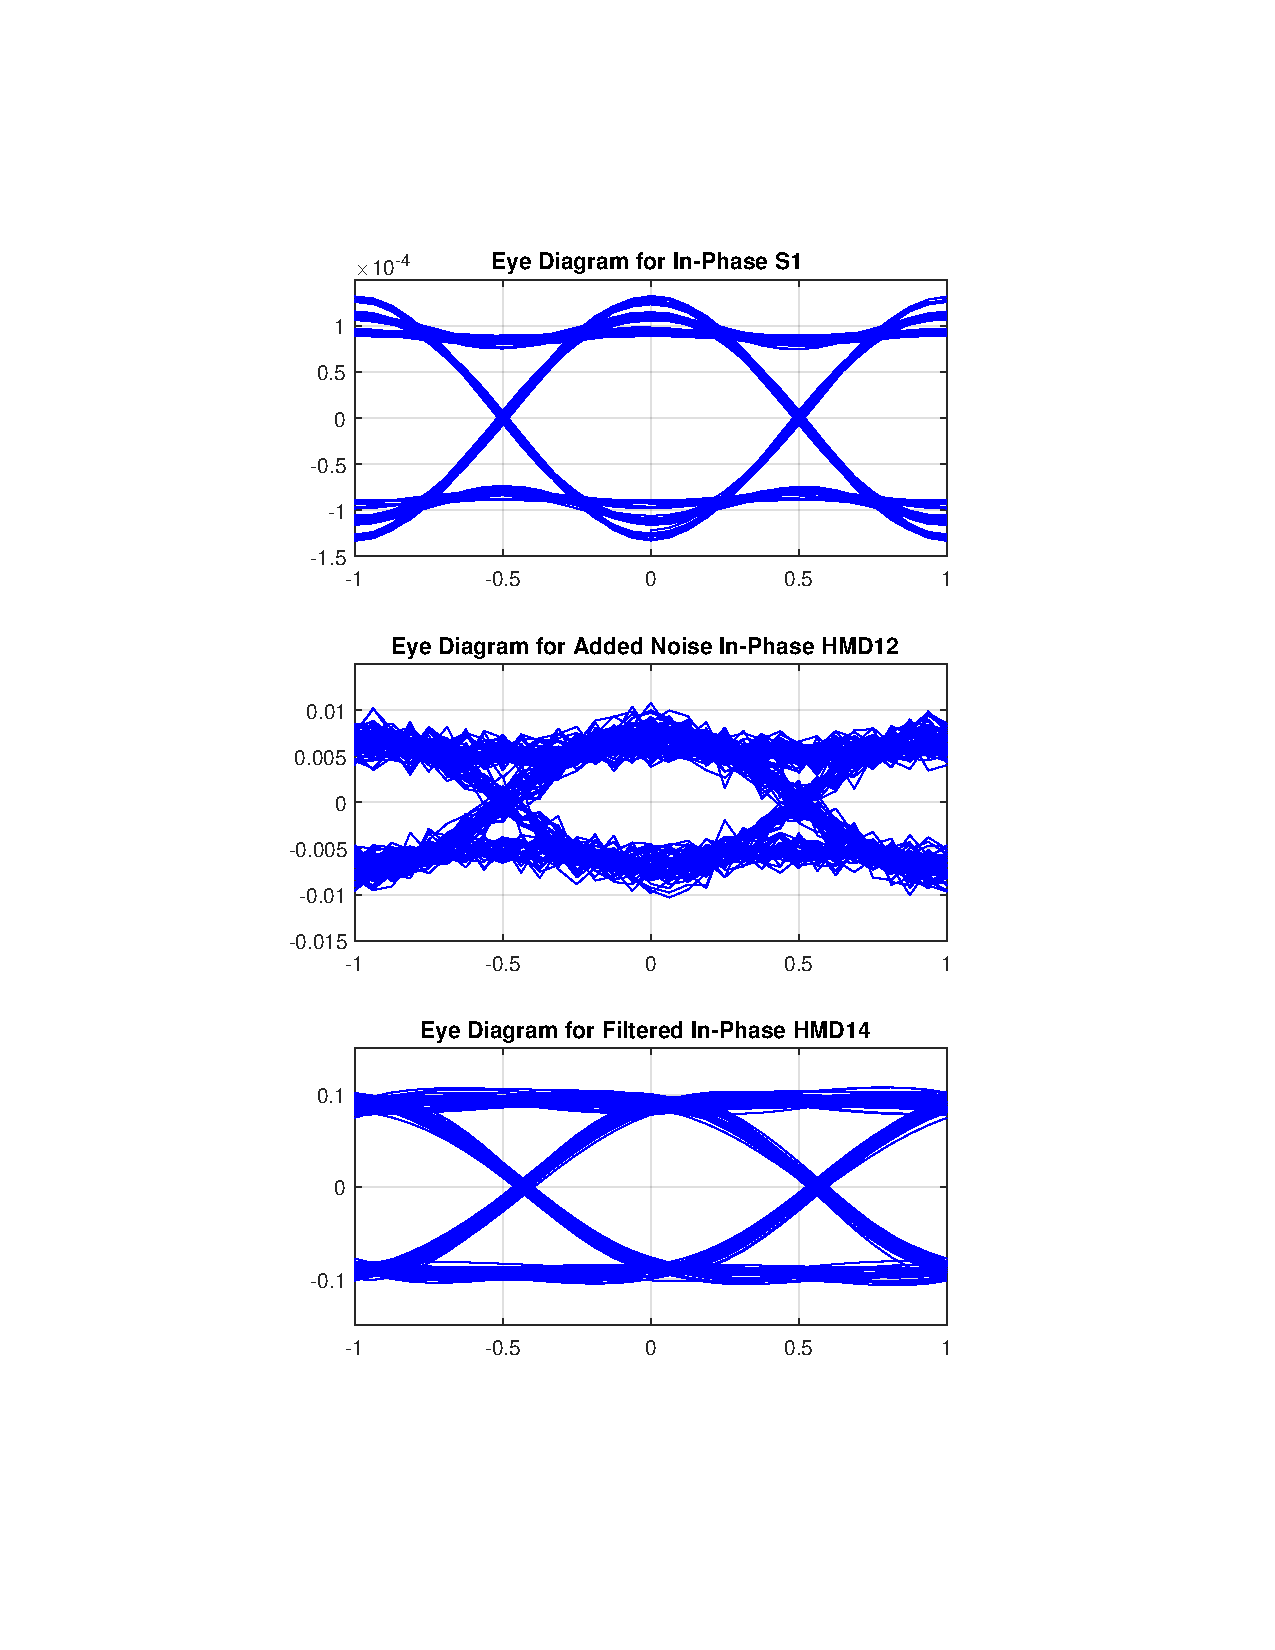
\includegraphics[clip, trim=5cm 4cm 5cm 4cm, width=\textwidth]{./sdf/m_qam_system/figures/eyes/if_p_45_09.pdf}
	\end{subfigure}
	\begin{subfigure}{.45\textwidth}
		\centering
		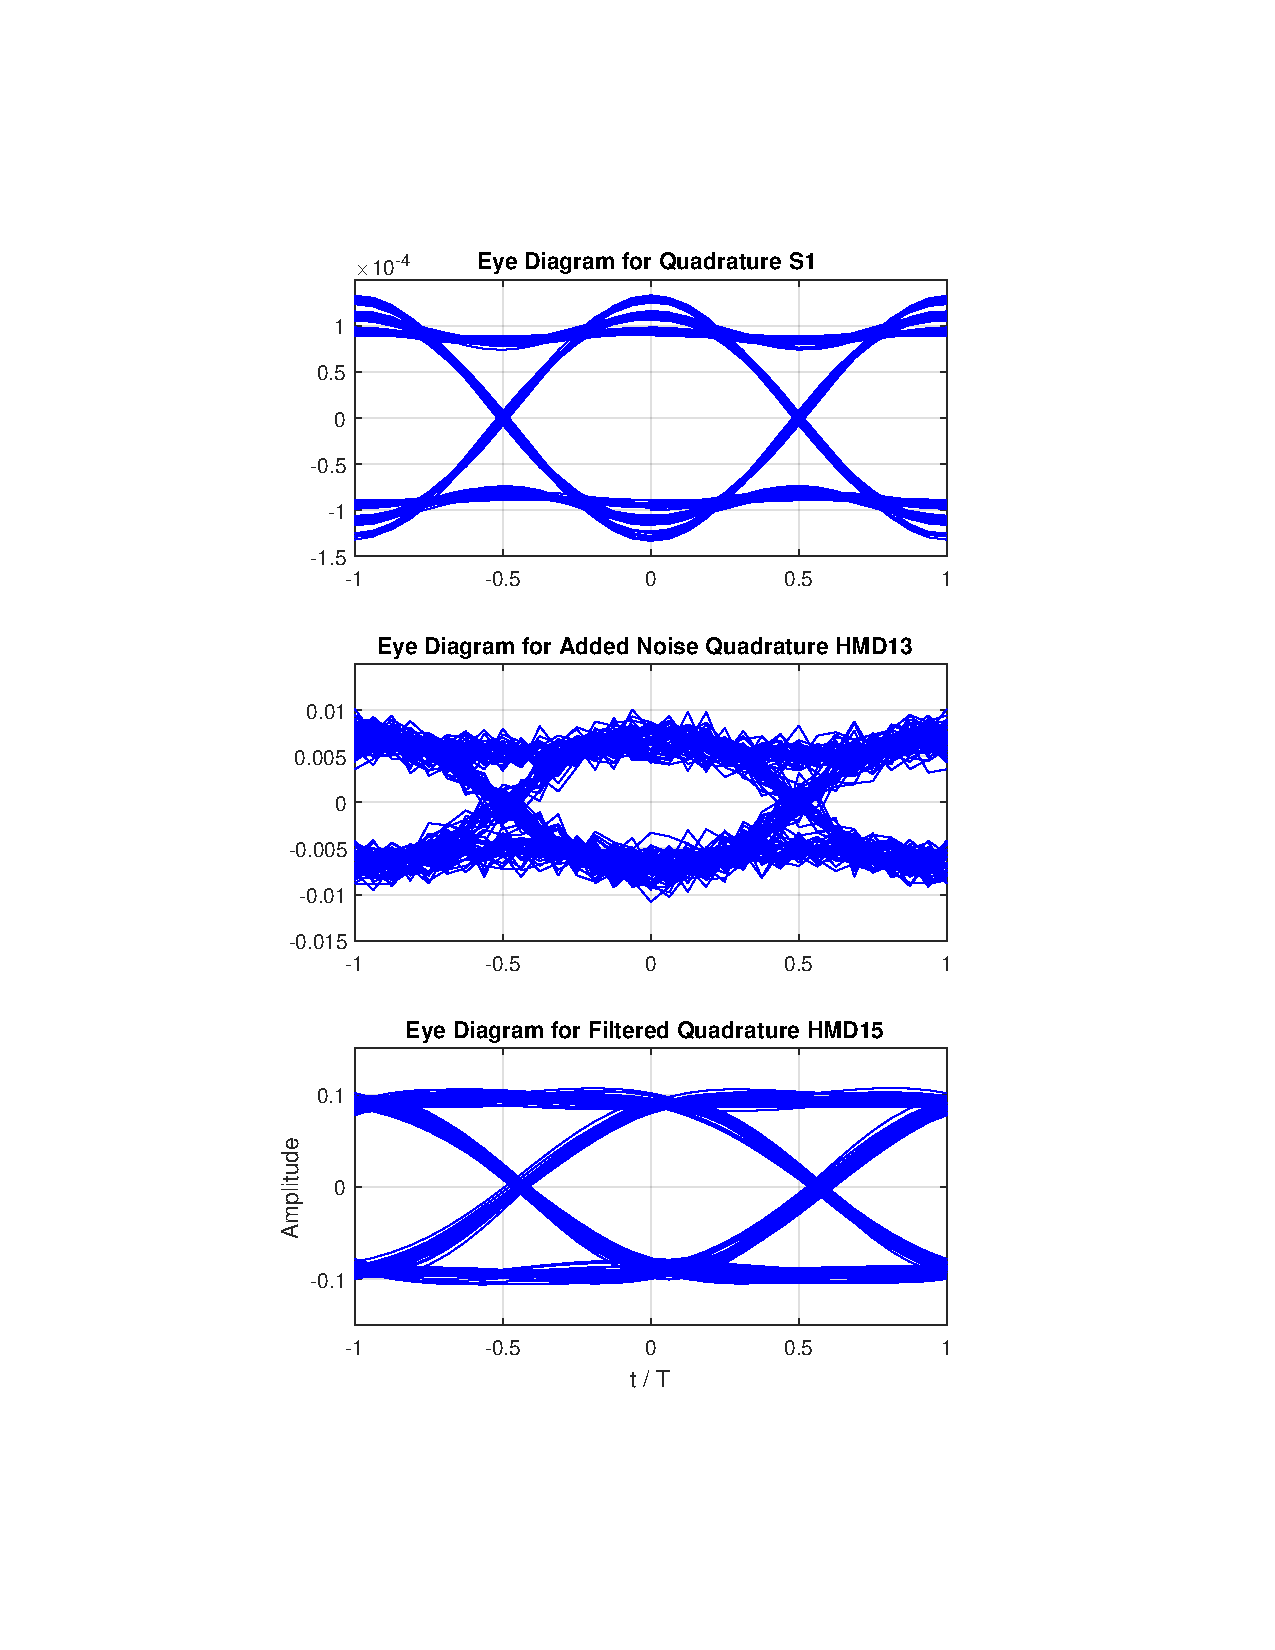
\includegraphics[clip, trim=5cm 4cm 5cm 4cm, width=\textwidth]{./sdf/m_qam_system/figures/eyes/q_p_45_09.pdf}
	\end{subfigure}
	
	\caption{Eye diagrams using matched filtering with root-raised-cosine
		at three different points: the optical output signal S1 on the top; the
		amplified signal with added noise at the middle, HMD12 and HMD13 for both
		components; and after passing through the last root-raised-cosine filter, HMD14
		and HMD15, for both components. Obtained through simulation with an optical
		power output of -45 dBm, 0 dBm at the local oscillator, a gain of $10^3$ at the
		amplifier, a noise spectral density of $10^{-6}$ and a rolloff factor of
		0.9.\label{fig:eyes_n_rrc_45_09}}
\end{figure}


Figures~\label{fig:eyes_n_rc_45_03} and~\label{fig:eyes_n_rrc_45_03} show the
cases described above, but with a roll-off factor of 0.3. It can be seen that
the case is in all aspects similar to the one presented above.


\begin{figure}[H]
	\centering
	\begin{subfigure}{.45\textwidth}
		\centering
		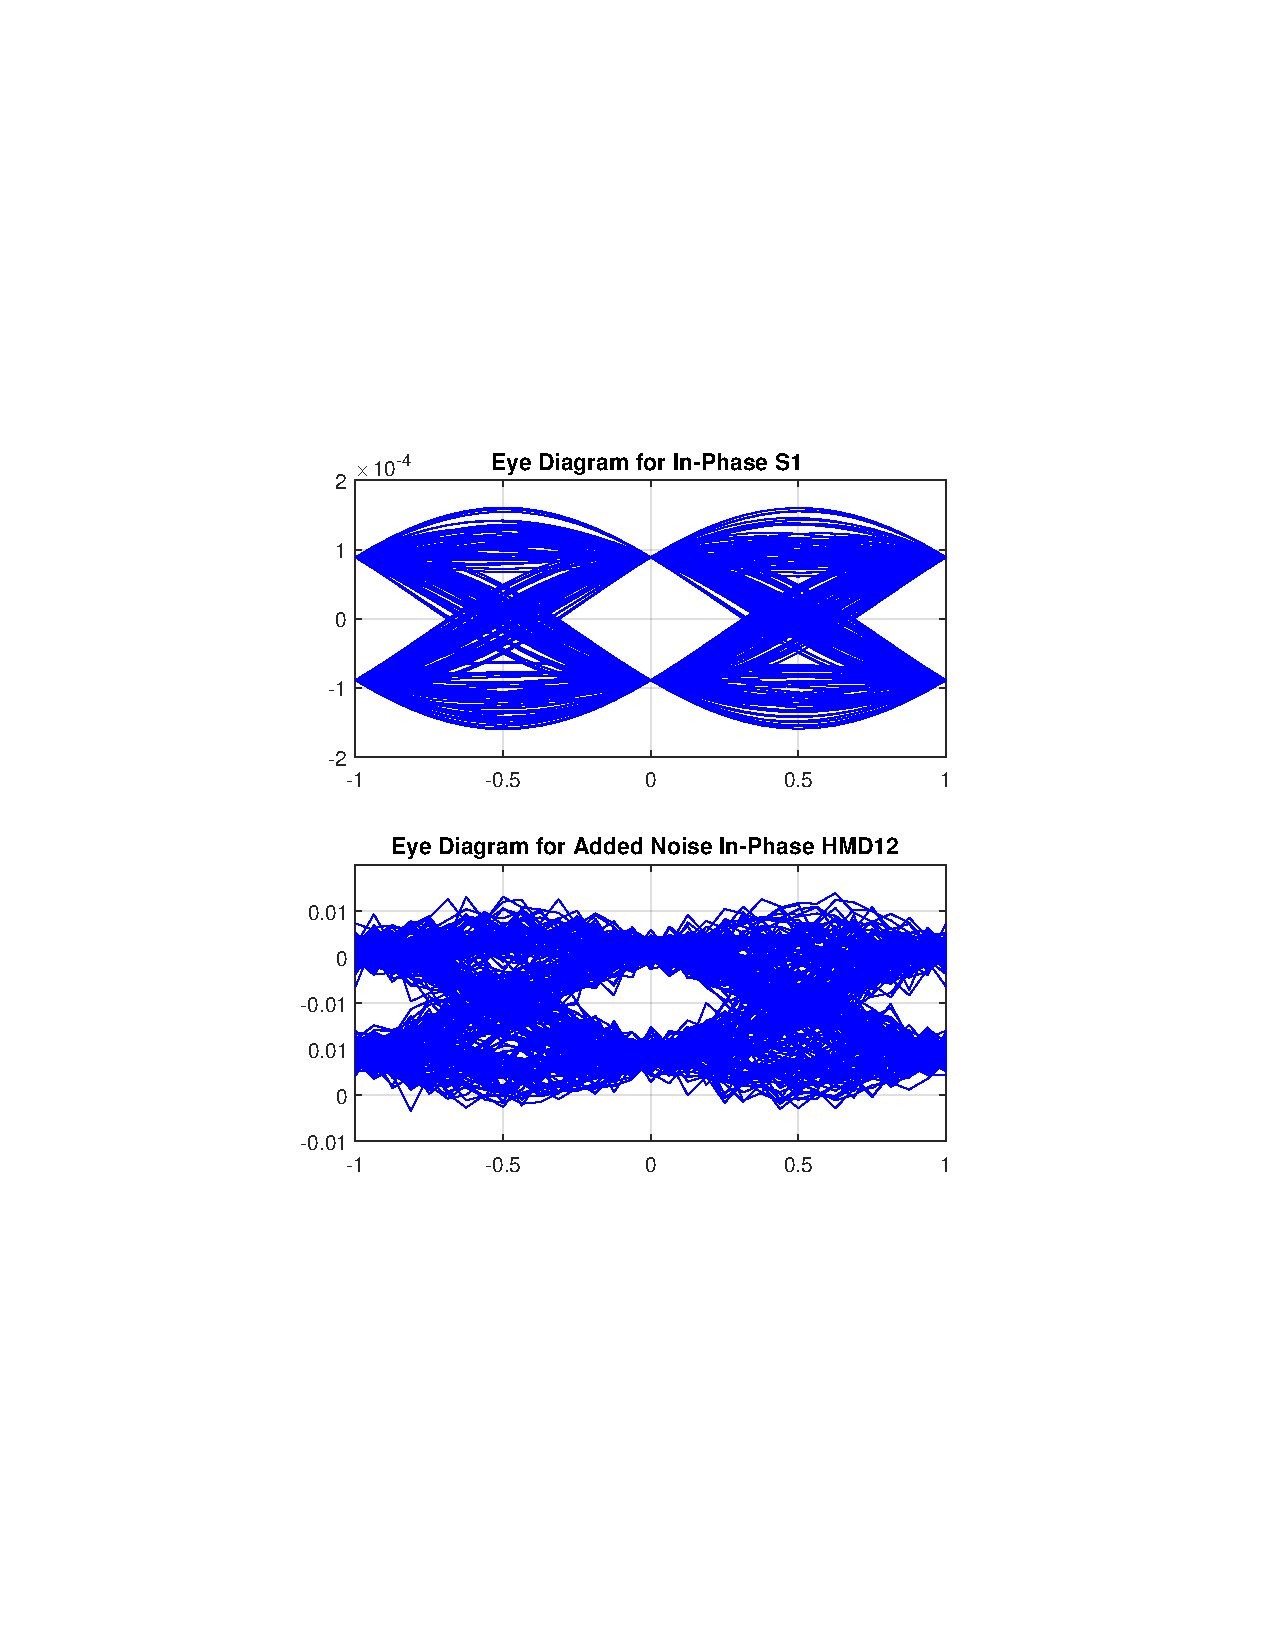
\includegraphics[clip, trim=5cm 4cm 5cm 4cm, width=\textwidth]{./sdf/m_qam_system/figures/eyes/if_n_nmf_45_60_rc.pdf}
	\end{subfigure}
	\begin{subfigure}{.45\textwidth}
		\centering
		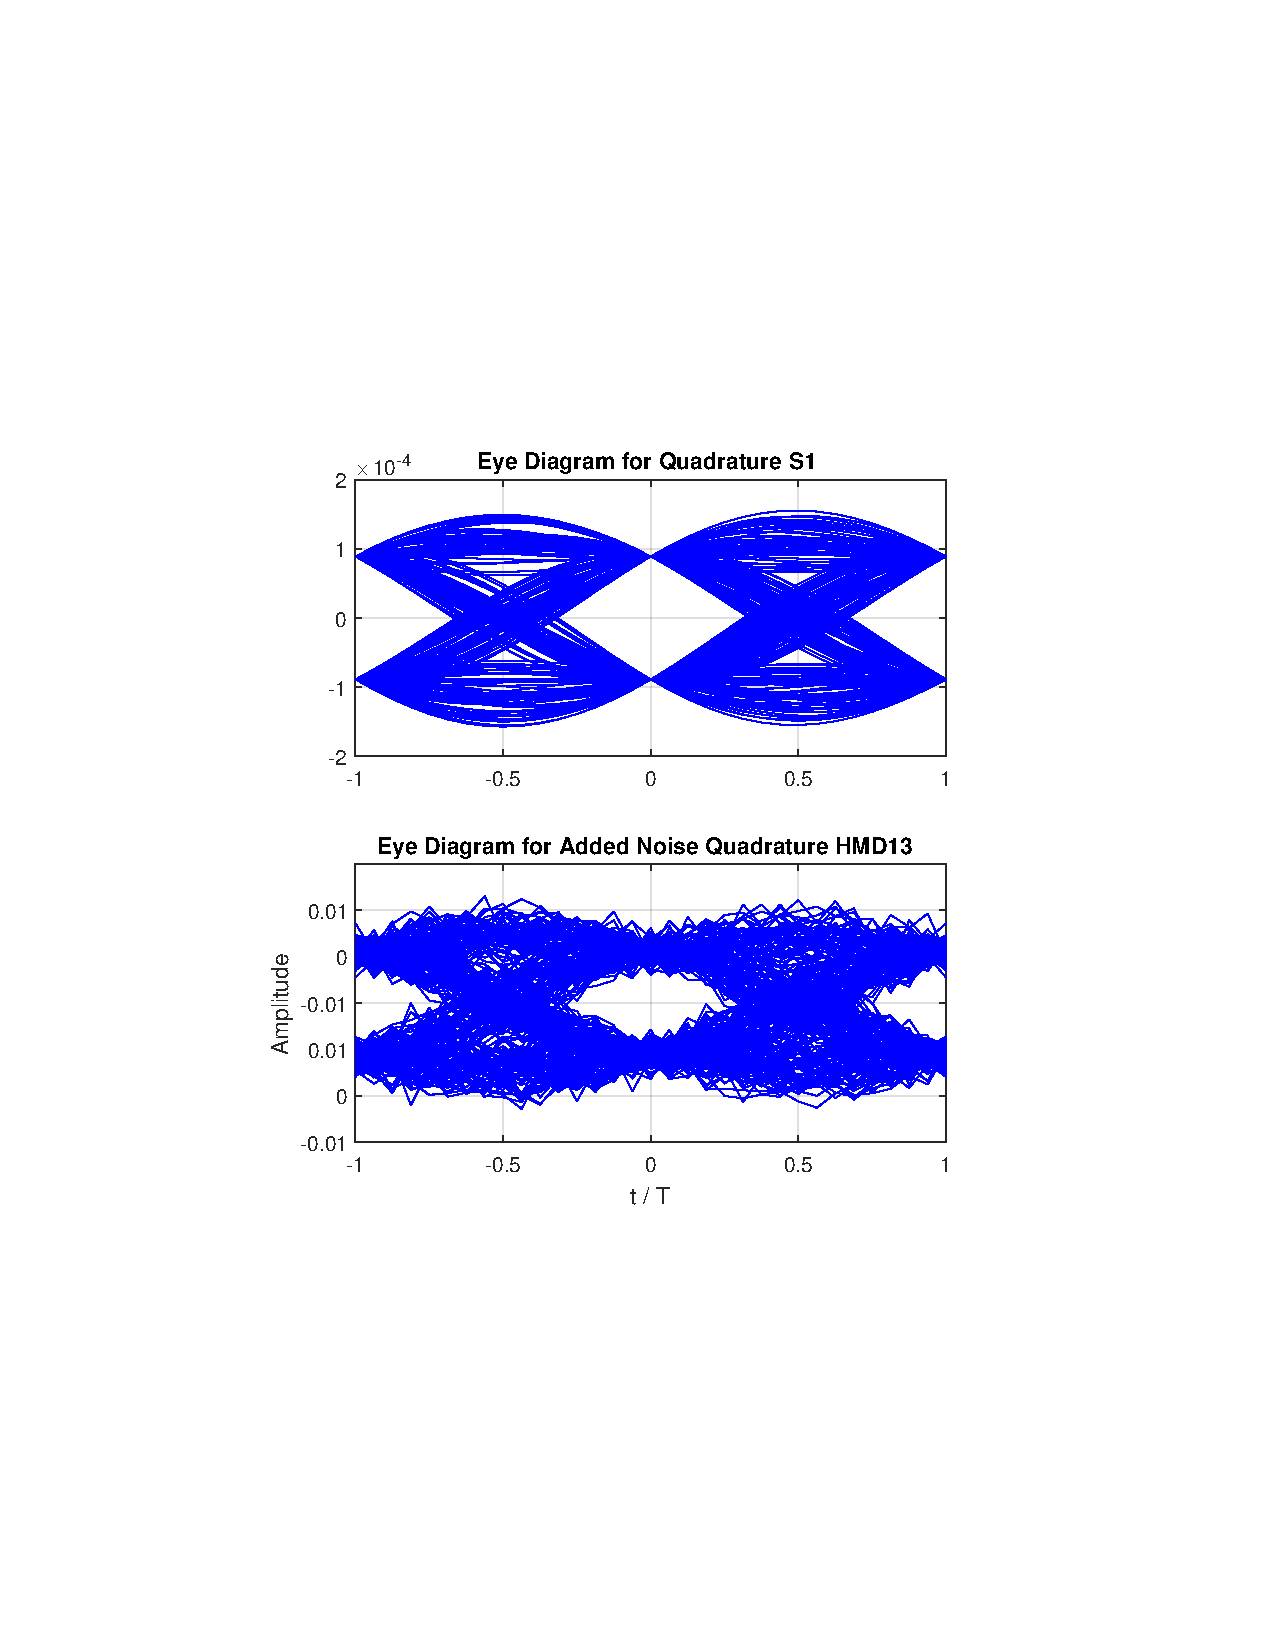
\includegraphics[clip, trim=5cm 4cm 5cm 4cm, width=\textwidth]{./sdf/m_qam_system/figures/eyes/q_n_nmf_45_60_rc.pdf}
	\end{subfigure}
	
	\caption{Eye diagrams without matched filtering with raised-cosine at
		two different points: the optical output signal S1 on the top and the amplified
		signal with added noise at the middle, HMD12 and HMD13, for
		both components. Obtained through simulation with an optical power output of
		-45 dBm, 0 dBm at the local oscillator, a gain of $10^3$ at the amplifier, a
		noise spectral density of $10^{-6}$ and a rolloff factor of
		0.3.\label{fig:eyes_n_rc_45_03}}
\end{figure}

\begin{figure}[H]
	\centering
	\begin{subfigure}{.45\textwidth}
		\centering
		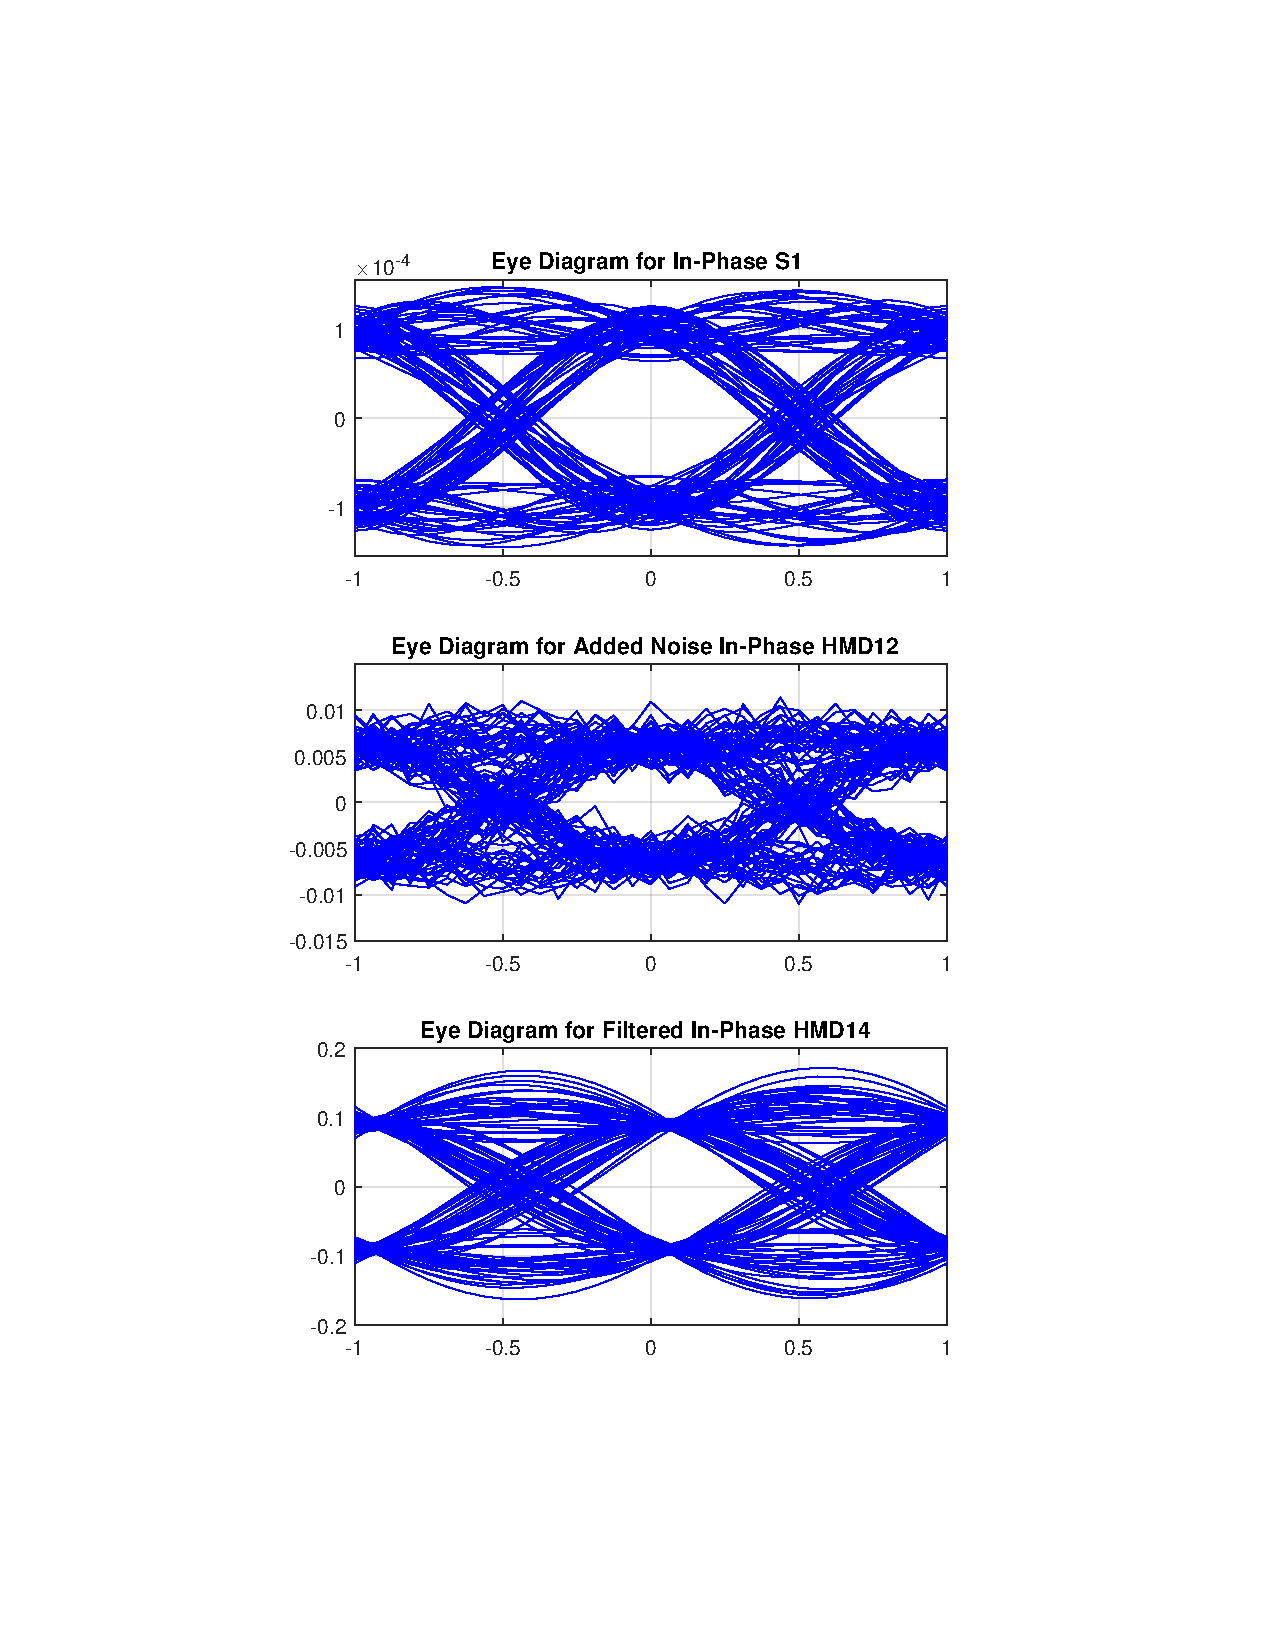
\includegraphics[clip, trim=5cm 4cm 5cm 4cm, width=\textwidth]{./sdf/m_qam_system/figures/eyes/if_p_45_03.pdf}
	\end{subfigure}
	\begin{subfigure}{.45\textwidth}
		\centering
		\includegraphics[clip, trim=5cm 4cm 5cm 4cm, width=\textwidth]{./sdf/m_qam_system/figures/eyes/q_p_45_03.pdf}
	\end{subfigure}
	
	\caption{Eye diagrams using matched filtering with root-raised-cosine
		at three different points: the optical output signal S1 on the top; the
		amplified signal with added noise at the middle, HMD12 and HMD13 for both
		components; and after passing through the last root-raised-cosine filter, HMD14
		and HMD15, for both components. Obtained through simulation with an optical
		power output of -45 dBm, 0 dBm at the local oscillator, a gain of $10^3$ at the
		amplifier, a noise spectral density of $10^{-6}$ and a rolloff factor of
		0.3.\label{fig:eyes_n_rrc_45_03}}
	
\end{figure}



\subsubsection*{Signals with AWGN and low SNR}
Figures \ref{fig:eyes_n_rrc_60_03}-\ref{fig:eyes_n_rc_60_09} show eye
diagrams similar to the previous section, but with a lower optical power ($-60~dBm$),
comparable to the spectral density of the noise ($10^{-6}$).



Figures~\ref{fig:eyes_n_rc_60_09} and~\ref{fig:eyes_n_rrc_60_09} show the
diagrams obtained without matched filtering and with matched filtering,
respectively, both using a roll-off factor of 0.9.

In this example the effects of matched filtering is even more obvious, as
without it the signal visually appears to be random noise.

\begin{figure}[H]
	\centering
	\begin{subfigure}{.45\textwidth}
		\centering
		\includegraphics[clip, trim=5cm 4cm 5cm 4cm, width=\textwidth]{./sdf/m_qam_system/figures/eyes/if_n_nmf_60_60_rc_09.pdf}
	\end{subfigure}
	\begin{subfigure}{.45\textwidth}
		\centering
		\includegraphics[clip, trim=5cm 4cm 5cm 4cm, width=\textwidth]{./sdf/m_qam_system/figures/eyes/q_n_nmf_60_60_rc_09.pdf}
	\end{subfigure}
	
	\caption{Eye diagrams without matched filtering with raised-cosine at
		two different points: the optical output signal S1 on the top and the amplified
		signal with added noise at the middle, HMD12 and HMD13 for both
		components. Obtained through simulation with an optical power output of -60
		dBm, 0 dBm at the local oscillator, a gain of $10^3$ at the amplifier, a noise
		spectral density of $10^{-6}$ and a rolloff factor of
		0.9.\label{fig:eyes_n_rc_60_09}}
\end{figure}


\begin{figure}[H]
	\centering
	\begin{subfigure}{.45\textwidth}
		\centering
		\includegraphics[clip, trim=5cm 4cm 5cm 4cm, width=\textwidth]{./sdf/m_qam_system/figures/eyes/if_p_60_09.pdf}
	\end{subfigure}
	\begin{subfigure}{.45\textwidth}
		\centering
		\includegraphics[clip, trim=5cm 4cm 5cm 4cm, width=\textwidth]{./sdf/m_qam_system/figures/eyes/q_p_60_09.pdf}
	\end{subfigure}
	
	\caption{Eye diagrams using matched filtering with root-raised-cosine at three different points: the optical output signal S1 on the top; the amplified signal with added noise at the middle, HMD12 and HMD13 for both components; and after passing through the last root-raised-cosine filter, HMD14 and HMD15, for both components. Obtained through simulation with an optical power output of -60 dBm, 0 dBm at the local oscillator, a gain of $10^3$ at the amplifier, a noise spectral density of $10^{-6}$ and a rolloff factor of 0.9.\label{fig:eyes_n_rrc_60_09}}
	
\end{figure}


Figures~\ref{fig:eyes_n_rc_60_03} and~\ref{fig:eyes_n_rrc_60_09} show the same
case but using a roll-off factor of 0.3.

\begin{figure}[H]
	\centering
	\begin{subfigure}{.45\textwidth}
		\centering
		\includegraphics[clip, trim=5cm 4cm 5cm 4cm, width=\textwidth]{./sdf/m_qam_system/figures/eyes/if_n_nmf_60_60_rc_03.pdf}
	\end{subfigure}
	\begin{subfigure}{.45\textwidth}
		\centering
		\includegraphics[clip, trim=5cm 4cm 5cm 4cm, width=\textwidth]{./sdf/m_qam_system/figures/eyes/q_n_nmf_60_60_rc_03.pdf}
	\end{subfigure}
	
	\caption{Eye diagrams without matched-filtering with raised-cosine at
		two different points: the optical output signal S1 on the top and the amplified
		signal with added noise at the middle, HMD12 and HMD13 for both components.
		Obtained through simulation with an optical power output of -60 dBm, 0 dBm at
		the local oscillator, a gain of $10^3$ at the amplifier, a noise spectral
		density of $10^{-6}$ and a rolloff factor of 0.3.\label{fig:eyes_n_rrc_60_03}}
	
\end{figure}

\begin{figure}[H]
	\centering
	\begin{subfigure}{.45\textwidth}
		\centering
		\includegraphics[clip, trim=5cm 4cm 5cm 4cm, width=\textwidth]{./sdf/m_qam_system/figures/eyes/if_p_60_03.pdf}
	\end{subfigure}
	\begin{subfigure}{.45\textwidth}
		\centering
		\includegraphics[clip, trim=5cm 4cm 5cm 4cm, width=\textwidth]{./sdf/m_qam_system/figures/eyes/q_p_60_03.pdf}
	\end{subfigure}
	
	\caption{Eye diagrams using matched filtering with root-raised-cosine
		at three different points: the optical output signal S1 on the top; the
		amplified signal with added noise at the middle, HMD12 and HMD13 for both
		components; and after passing through the last root-raised-cosine filter, HMD14
		and HMD15, for both components. Obtained through simulation with an optical
		power output of -60 dBm, 0 dBm at the local oscillator, a gain of $10^3$ at the
		amplifier, a noise spectral density of $10^{-6}$ and a rolloff factor of
		0.3.\label{fig:eyes_n_rc_60_03}} 
\end{figure}



\subsection{BER Curves}

The simulated results show agreement with the theoretical curves, as can be seen in Figure~\ref{fig:ber_pseudorandom}.
\begin{figure}[H]
	\centering
	\includegraphics[clip, trim=4cm 8cm 4cm 8cm, width=0.7\textwidth]{./sdf/m_qam_system/figures/teor_vs_simul.pdf}
	\caption{Simulation results for a random binary sequence with $40000$ bits, a noise power of $10^{-6}$ and an amplification of $10^3$. The simulated values which used a matched filter were obtained by shaping the pulse with a root-raised-cosine FIR filter and filtering the signal before the sample with the same filter. The results without matched filtering were obtained by using shaping the pulses with a raised-cosine filter. The margins shown were obtained for a 95\% confidence level.}
	\label{fig:ber_pseudorandom}
\end{figure}% 


\subsection*{Experimental Analysis}
\begin{figure}[H]
	\centering
	\includegraphics[width=0.8\textwidth]{./sdf/m_qam_system/figures/mqamExperimental20180206.pdf}
	\caption{Experimental setup}
	\label{fig:experimental_mqam_setup}
\end{figure}
%
%
\begin{table}[H]
	\centering
	\begin{tabulary}{1.0\textwidth}{|L|L|l|}
%		\hline
%		\textbf{Device}		& \textbf{Description}\\
%		\hline
%		Balanced Photodetector	& Thorlabs PDB 450C\\
%		\hline
%%		BS					& Beam Splitter\\
%		\hline
%%		Pulse Generator		& HP 8116A Pulse Generator\\
%		\hline
%%		Amplitude Modulator	& Mach Zehnder SDL OC 48\\
%		\hline
%%		VOA					& Eigenlicht Power Meter 420\\
%		\hline
%%		VOA					& Thorlabs VOA 45-APC\\
%%		\hline
%%		PIN					& Thorlabs PDB 450C\\
%		\hline
%%		ADC					& Picoscope 6403D\\
%		\hline
	\end{tabulary}
\end{table}


\subsection{Comparative Analysis}

In this section we show the simulation results and compared them with the theoretical predictions for an M-QAM system with $M=4$. Figure \ref{fig:ber_pseudorandom} shows the variation of the BER with the optical power of the signal, using $40000$ bits produced by a random number generator. The noise power was set at $10^{-6}$, the local oscillator at $0~dBm$ and the amplification at the transimpedance amplifier was set at $10^3$.
The blue line represents the theoretical curve, while the orange points represent the simulated values with the respective confidence margins. The simulation agrees closely with the theoretical values.



%\begin{figure}[h]
%	\centering
%	\includegraphics[clip, trim=4cm 8cm 4cm 8cm, width=0.7\textwidth]{./sdf/m_qam_system/figures/BER_QPSK_sim_mf_20180205.pdf}
%	\caption{Simulation result using root-raised cosine matched filtering for a random binary sequence with $40000$ bits, a noise power of $10^{-6}$ and an amplification of $10^3$.}
%	\label{fig:ber_pseudorandom_mf}
%\end{figure}% 


\subsection{Open Issues}

\newpage


%%%%%%%%%%%%%%%%%%%%%%%%%%%%%%%%%%%%%%%%%%%%%%%%%%%%%%%%%%%%%%%%%%%%%%%%%%%%%%%%%%%%%%%%%%%%%%%%%%%%%%%%%%%%
% References
%%%%%%%%%%%%%%%%%%%%%%%%%%%%%%%%%%%%%%%%%%%%%%%%%%%%%%%%%%%%%%%%%%%%%%%%%%%%%%%%%%%%%%%%%%%%%%%%%%%%%%%%%%%%

\renewcommand{\bibname}{References}
%
\bibliographystyle{myIEEEtran}
% argument is your BibTeX string definitions and bibliography database(s)
\bibliography{./sdf/m_qam_system/m_qam_system}
%
%


\cleardoublepage
 \fi
\ifdefined\sdf          \clearpage
\section{Simplified Coherent Receiver}

\begin{tcolorbox}	
\begin{tabular}{p{2.75cm} p{0.2cm} p{10.5cm}} 	
\textbf{Student Name}  &:& Romil Patel\\
\textbf{Starting Date} &:& August 16, 2017\\
\textbf{Goal}          &:& Develop a simplified structure (low cost) for a coherent receiver, that can be used in coherent PON, inter-data center connections, or metropolitan networks (optical path lengths < 100 km).
\end{tabular}
\end{tcolorbox}

%In recent days, homodyne detection has been discussed and investigated a lot due to the advancement in the DSP in the electrical domain. However, a major drawback of homodyne detection is the incoming signal should be separated into inphase and quadrature (I/Q) signals in the optical domain. Therefore, it demands more hardware to accommodate the requirement of the signal separation  in the optical domain. For instance, 4 balanced photodetectors with double hybrid structures and 4-channel ADCs are required.
%On the other hand, heterodyne receiver simplifies the detection scheme to some extent with the requirement of having only half of photodetectors and ADC.\\
In the optical communication, coherent detection scheme constitute the solution for the medium-to-long-reach application; however, the cost of coherent receiver becomes a major obstacle in the case of short-reach links applications like PON, inter-data-center communications, metropolitan network etc. In order to get rid of higher cost and to make the transceiver more applicable in short-reach links, a new architecture of optical receiver has been proposed which combines the advantages of coherent transmission and cost effectiveness of direct detection. The working principle of the receiver is based on the famous Kramers-Kronig(KK) relationship which facilitates digital post-compensation of linear propagation impairments.
\subsection{Kramers-Kronig receiver}
The key concept behind the Kramers-Kronig self coherent receiver is to aquire "\textit{minimum phase single sideband signal}".



\subsubsection{1. What are the requirements for the KK receiver scheme?}
The Kramers-Kronig receiver based communication scheme relies on identifying a condition which ensures that \textbf{the received signal is minimum phase}, in such a case its phase can be uniquely extracted from its intensity.\\ In order to facilitate the extraction of phase information from the intensity of the received minimum phase signal, it is prerequisite that the transmitted signal should be \textbf{analytical signal} in which real and imaginary parts are related to each other by means of Hilbert transform of each other.   

\subsubsection{2. What is minimum phase signal?}
A necessary and sufficient condition for a signal $E(t)$ to be minimum phase is that the curve described by $E(t)$ when $t\rightarrow -\infty$ to $t\rightarrow \infty$ \textbf{does not encircle the origin}.

\subsubsection{3. what is Analytical Signal?}
An analytic signal is a complex-valued signal that has no negative frequency components, and its real and imaginary parts are related to each other by the Hilbert transform.
\begin{equation}
s_a(t)=s(t)+i\hat{s}(t)
\label{Analytical signal}
\end{equation}
where, $s_a(t)$ is an analytical signal and $\hat{s}(t)$ is the Hilbert transform of the signal ${s}(t)$. Such analytical signal can be used to generate Single Sideband Signal (SSB) signal(See the Appendices).

\subsubsection{4. How we can use these signals and profit from them?}
This section represents the justification that why we need to use these signals into our proposed transceiver system.\\
\textbf{Analytical Signal:}\\
Analytical signal used for generating single sidebnad (SSB) signal. In the case of a SSB signal $u(t)$ described as,
\begin{equation}
u(t)=u_r(t)+iu_i(t)
\label{5.15}
\end{equation}
the real part $U_r(t)$  and the imaginary parts $U_i(t)$ are Hilbert transform of each other.
\begin{equation}
\begin{split}
u_r(t) &=-\frac{1}{\pi} p.v. \int_{-\infty}^{\infty} \frac{u_i(t')}{t-t'} dt' \\
u_i(t) &=\frac{1}{\pi} p.v. \int_{-\infty}^{\infty} \frac{u_r(t')}{t-t'} dt' \\
\end{split}
\label{Eq:5.24}
\end{equation}
These relations are known as Kramers-Kronig relation. Alternatively we can define both these relationship into the following form,
\begin{equation}
\begin{split}
u(t) &=\frac{i}{\pi} p.v. \int_{-\infty}^{\infty} \frac{u(t')}{t-t'} dt' 
\end{split}
\label{Eq:5.24}
\end{equation}\\
\textbf{Minimum Phase signal:}\\
If the trajectory of the received SSB signal never encircles the origin for $t\epsilon(-\infty,\infty)$






















%The communication scheme discussed here relies on the identifying a specific condition that ensures the received signal is minimum phase. This condition facilitates the unique way to extract the phase of the received signal from its intensity. If we denote s(t) as a complex data-carrying signals whose spectrum is contained between -B/2 to B/2, and consider a single sideband signal of the form,
%\begin{equation}
%h(t)=A+s(t)exp(i\pi Bt)
%\end{equation}
%Where $A$ is a constant. Here, Nyquist stability criterion can be used to ensure that $s(t)$ is a minimum phase signal. The condition of minimum phase signal is satisfied when $|A|>|s(t)|$ by guaranteeing Nyquist stability of the received signal.
%When $h(t)$ is a minimum-phase signal, its phase $\phi(t)$ and absolute value $|h(t)|$ are uniquely related by Hilbert transform:
%\begin{equation}
%	\phi(t)=\frac{1}{\pi}  p.v. \int_{-\infty}^{\infty} dt' \frac{log[|h(t')|]}{t-t'}
%	\label{Eq:5.15}
%\end{equation}
%where \textit{p.v.} stands for \textit{principal value}. The relationship depicted in Equation \ref{Eq:5.15} can also be conveniently implemented in frequency domain as,
%\begin{equation}
%\tilde{\phi}(\omega)=i sign(\omega) \mathcal{F} \{log[|h(t)|]\}
%\label{Eq:5.16}
%\end{equation}
%where $sign(\omega)$ is the sign function which is equal to 1 when $\omega>0$, to 0 when $\omega=0$ and to -1 when $\omega<0$. Symbol $\mathcal{F}$ denotes the Fourier transform.
\begin{figure}[h]
	\centering
	\includegraphics[width=1.0\textwidth, height=7cm]{./sdf/simplified_coherent_receiver/figures/Single_Polarization_Tx.pdf}
	\caption{Transmitter}\label{Transmitter}
\end{figure}

\subsection{KK Scheme}
If we consider the complex envelope of the incoming electric field by $E_s(t)$ confined within the optical bandwidth denoted by B. The LO assumed to be a continuous wave (CW) signal whose amplitude is $E_0$ whose frequency coincides with the left edge of the information-carrying signal spectrum. Here, we assumed that $E_0$ is real-valued and positive, which is equivalent to referring all phase value to that of LO.\\
The complex envelope of the field striking upon the photo-diode can be given as,
\begin{equation}
E(t)=E_s(t)+E_0 exp(i\pi Bt)
\end{equation}
The photo current $I$ produced by the photo-diode is proportional to the field intensity $I=|E(t)|^2$, here proportionality constant considered as 1 for the sake of simplicity. If $E_0$ is large enough to ensure that the signal $E(t)exp(i\pi Bt)=E_0+E_s(t)exp(-i\pi Bt)$ is minimum phase. Equations \ref{Eq:5.15} and \ref{Eq:5.16} can be used to reconstruct the signal $E_s(t)$ as follows:
\begin{equation}
E_s(t)=\{\sqrt{I(t)} exp[i\phi_E(t)]-E_0\} exp(i\pi Bt)
\end{equation}
\begin{equation}
\phi_E(t)=\dfrac{1}{2\pi} p.v. \int_{-\infty}^{\infty} dt' \frac{log[|I(t')|]}{t-t'}
\label{Eq:5.19}
\end{equation}
Here, the average value of the phase returned by Equation \ref{Eq:5.19} is zero, which implies the need for an additional phase-recovery procedure. 
\begin{figure}[h]
	\centering
	\includegraphics[width=1.0\textwidth, height=8cm]{./sdf/simplified_coherent_receiver/figures/detailed_subsystem.pdf}
	\caption{Tx/Rx DSP main subsystem}\label{DSP_main_subsystem}
\end{figure}

\subsection{Tx side}
Single polarization 16QAM signals (1.25 Gbaud) to be generated at the Tx through an IQ modulator (Figure \ref{DSP_main_subsystem}). The IQ modulated signal is then applied to the Hilbert transformer which generates the imaginary part for our analytical signal. In analytical signal, real and imaginary parts are related to each other by Hilbert transform and it has no negative frequency contents. Such analytical signal can be used for generating bandwidth efficient single sideband (SSB) signal.





\subsubsection{SSB Signal generation using Hilbert transformation}
This section describes the SSB signal generation using Hilbert transformation method (Phase Shift Method). Consider a message signal $m(t)$ with its frequency domain spectrum $M(F)$ as shown in Figure\ref{Original_baseband_signal}. From the Figure \ref{Original_baseband_signal}, we can see that both the side are scaled by factor '1' which means it represents the original signal.
\begin{figure}[h]
	\centering
	\includegraphics[width=1.0\textwidth, height=8cm]{./sdf/simplified_coherent_receiver/figures/SSB1.pdf}
	\caption{Original baseband signal}\label{Original_baseband_signal}
\end{figure}\\ 	
Now let's consider the modulated signal $x(t)$ given as,
\begin{equation}
x(t)=m(t) cos(2\pi f_c t)
\label{Eq:5.20}
\end{equation}
Frequency domain representation of the equation \ref{Eq:5.20} can be given as,
\begin{equation}
X(F)=\frac{1}{2}M(f-f_c)+\frac{1}{2}M(f+f_c)
\label{Eq:5.21}
\end{equation}
Here in equation \ref{Eq:5.21}, we can observe that each side band are scaled by $\dfrac{1}{2}$ on the frequency spectrum. Figure displays the frequency domain representation of the modulated signal $X(F)$.
\begin{figure}[h]
	\centering
	\includegraphics[width=1.0\textwidth, height=8cm]{./sdf/simplified_coherent_receiver/figures/SSB2.pdf}
	\caption{Original modulated signal}\label{Original_modulated_signal}
\end{figure}\\ 
Next, we will discuss something more interesting which is called as Hilbert transform of the original message signal $m(t)$. As we discussed earlier, in the frequency domain, the Hilbert transformed signal $\hat{M}(f)$ can be achieved by multiplying the Fourier transformed signal $M(F)$ with $[-j sgn(F)]$.
\begin{figure}[h]
	\centering
	\includegraphics[width=1.0\textwidth, height=8cm]{./sdf/simplified_coherent_receiver/figures/SSB3.pdf}
	\caption{Hilbert transformed modulated signal}\label{Hilbert_Transformed_signal}
\end{figure}
Suppose we modulate the Hilbert transformed message signal $\hat{m}(t)$  with the $sin(2\pi f_c t)$ (quadrature phase carrier), then we get the following results:

\begin{equation}
\begin{split}
{\hat{m}(t)} sin(2\pi f_c t)&={\hat{m}(t)}\frac{e^{j2\pi f_c t} - e^{-j2\pi f_c t} }{2}\\
&={\hat{m}(t)}\frac{e^{j2\pi f_c t}}{2} - {\hat{m}(t)}\frac{e^{-j2\pi f_c t}}{2}\\
&={\frac{\hat{M}(f-f_c)}{2j}}-{\frac{\hat{M}(f+f_c)}{2j}}\\
&={\frac{-j}{2}\hat{M}(f-f_c)}+{\frac{-j}{2}\hat{M}(f+f_c)}\\
\end{split}
\label{5.22}
\end{equation}
The detailed explanation of the equation \ref{Eq:5.22} has been described in the Figure \ref{Hilbert_Transformed_modulated_signal} and \ref{Hilbert_Final}. Figure \ref{Hilbert_Transformed_modulated_signal} displays the spectrum of the $\hat{M}(f+f_c)$ and $\hat{M}(f-f_c)$ for the positive and negative frequencies respectively. The final equation resolution of equation displays that both positive and negative side of the spectrum multiplied with $\frac{j}{2}$ and $\frac{-j}{2}$ respectively. Finally the spectrum of the signal ${\hat{m}(t)} sin(2\pi f_c t)$ can be given as Figure \ref{Hilbert_Final}.
\begin{figure}[h]
	\centering
	\includegraphics[width=1.0\textwidth, height=8cm]{./sdf/simplified_coherent_receiver/figures/SSB4.pdf}
	\caption{Hilbert transformed modulated signal}\label{Hilbert_Transformed_modulated_signal}
\end{figure}

\begin{figure}[h]
	\centering
	\includegraphics[width=1.0\textwidth, height=8cm]{./sdf/simplified_coherent_receiver/figures/SSB5.pdf}
	\caption{Hilbert transformed modulated signal}\label{Hilbert_Final}
\end{figure}

Further, summation of the two signals ${m(t)} cos(2\pi f_c t)$ and ${\hat{m}(t)} sin(2\pi f_c t)$ will generate the upper sideband SSB signal as follows,
\begin{equation}
u(t)={m(t)} cos(2\pi f_c t)-{\hat{m}(t)} sin(2\pi f_c t)
\label{5.23}
\end{equation}
From the above discussion, the spectrum of the Equation \ref{5.23} can be given by the Figure \ref{SSB_signal_spectrum}. Similarly, for the lower sideband SSB can be generated by Equation,
\begin{equation}
u(t)={m(t)} cos(2\pi f_c t)+{\hat{m}(t)} sin(2\pi f_c t)
\label{5.24}
\end{equation}
\begin{figure}[h]
	\centering
	\includegraphics[width=1.0\textwidth, height=8cm]{./sdf/simplified_coherent_receiver/figures/SSB6.pdf}
	\caption{SSB signal spectrum}\label{SSB_signal_spectrum}
\end{figure}






  



\subsection{Rx side}
At the receiver side, signal is coherently detected using a simplified coherent receiver and a local oscillator. The optical signal is then converted into the electrical domain using two balanced photodetector (BPD), or alternatively four photodetector, and amplified by a transimpedance amplifier (TIA). Following that, the signals are sampled by two 8-bit 2.5 GSa/s ADC and the this digitized signal sent to the FPGA (Virtex-7) where all post-detection DSP implemented in real-time.

\begin{thebibliography}{9}
	\bibitem{latexcompanion}
	Antonio Mecozzi, Cristian Antonelli, and Mark Shtaif.
	\textit{Kramers-Kronig Coherent Receiver}.
	Optica, vol.3, no.11, 2016, p.1220., doi:10.1364/optica.3.001220.
	
	\bibitem{latexcompanion}
	Antonio Mecozzi.
	\textit{Retrieving the full optical response from amplitude data by Hilbert transform}. Opt. Comm. 282, 4183-4187.
	
	\bibitem{latexcompanion}
	Antonio Mecozzi.
	\textit{A necessary and sufficient condition for minimum phase and implication of phase retrieval}. arXiv:1606.04861.
\end{thebibliography}

\subsubsection{\textbf{APPENDICES}}
\textbf{Apppendix A}\\
In this section, we'll discuss the brief idea of generating SSB signal using Hilbert transform method. To understand this, we may express signal $u(t)$ as a summation of the two complex-valued functions.
\begin{equation}
s(t)=\dfrac{1}{2}[s(t)+j\hat{s}(t)]+\dfrac{1}{2}[s(t)-j\hat{s}(t)]
\label{}
\end{equation}
where, the term $\dfrac{1}{2}[s(t)+j\hat{s}(t)]$ is the analytical representation of the signal $s(t)$ (from Equation \ref{Analytical signal}). Another term represents the complex conjugate $\dfrac{1}{2}[s(t)-j\hat{s}(t)]$ of this analytical signal. Such representation of the signal ${s_a}(t)$ and ${s_a^*}(t)$ divide the signal into non-negative frequency component and non-positive frequency component respectively. Alternatively, we can write it as,
\begin{equation}
\dfrac{1}{2}{S_a}(f) = \begin{cases}
S(f) &\text{for $f>0$}\\
0    &\text{for $f<0$}\\
\end{cases}
\end{equation}
where ${S_a}(f)$ and ${S}(f)$ are the Fourier transform of ${t_a}(t)$ and ${s}(t)$ respectively. The frequency translated version of ${S_a}(f-f_0)$ contains only one side (positive) of ${S}(f)$ and hence it is called single sideband signal ${s_ssb}(t)$,
\begin{equation}
{F}^{-1}\{S_a(f-f_0)\}={s_a}(t) e^{j2\pi f_0 t}={s_{ssb}}(t)+j{\hat{s}_{ssb}(t)}
\end{equation}
Therefore, from the Euler's formula,
\begin{equation}
\begin{split}
{s}_{ssb}(t)&=Re\{s_a(t)  e^{j2\pi f_0 t}\}\\
&=Re\{[s(t)+j\hat{s}(t)] [cos(2\pi f_0t)+jsin(2\pi f_0t)]\}\\
&=s(t)cos(2\pi f_0t)-\hat{s}(t)sin(2\pi f_0t)
\end{split}
\label{USB_SSB}
\end{equation}
This Equation \ref{USB_SSB} displays the mathematical modeling of the upper sideband SSB signal. Similarly, we can generate lower sideband SSB signal by,
\begin{equation}
{s}_{ssb}(t)=s(t)cos(2\pi f_0t)+\hat{s}(t)sin(2\pi f_0t)
\label{LSB_SSB}
\end{equation}\\
\textbf{Apppendix B}\\
%\subsubsection{Kramers Kronig Relation}
Suppose we have a SSB signal $u(t)$ described as,
\begin{equation}
u(t)=u_r(t)+iu_i(t)
\label{Eq:5.22}
\end{equation}
In the equation \ref{Eq:5.22}, the real and imaginary parts $U_r(t)$ and $U_i(t)$ are related through the Kramers-Kronig relation with each other. An intuitive way to analyze the relation is based on expressing its Fourier transform $\tilde{U}(\omega)$ as follows,
\begin{equation}
\tilde{U}(\omega)=\dfrac{1}{2}[1+sgn(\omega)]\tilde{U}(\omega)
\label{Eq:5.23}
\end{equation}
The equation \ref{Eq:5.23} follows the SSB signal condition $\tilde{U}(\omega)=0$ for $\omega<0$. Further, simplification0n of the signal can be summarized as follows:
\begin{equation}
\begin{split}
\tilde{U}(\omega)&=\dfrac{1}{2}[1+sgn(\omega)]\tilde{U}(\omega)\\
&=\dfrac{1}{2}\tilde{U}(\omega)+\dfrac{1}{2}sgn(\omega)\tilde{U}(\omega)
\end{split}
\label{Eq:5.23}
\end{equation}
Taking inverse Fourier transform of the equation \ref{Eq:5.23},
\begin{equation}
\begin{split}
{u}(t)&=IFT\{\tilde{}(\omega)\}\\
&=\dfrac{1}{2}{u}(t)+\underline{\dfrac{1}{2}[IFT\{sgn(\omega)\} \circledast {u}(t)]}
\end{split}
\label{Eq:5.23}
\end{equation}
The underlined term in Equation \ref{Eq:5.23} displays that multiplication in frequency domain converted into the convolution in the time domain. Further, IFT of the function $sgn(\omega)$ given as $(-i/\pi t)$. As a consequences, we can further simplify our equation as,
\begin{equation}
\begin{split}
{u}(t)&=\dfrac{1}{2}{U}(t)+\frac{1}{2}\bigg[\frac{i}{\pi t} \circledast {u}(t) \bigg]\\
\frac{{u}(t)}{2} &=\frac{1}{2}\bigg[\frac{i}{\pi t} \circledast {u}(t) \bigg]\\
{u}(t) &=i\bigg[\frac{1}{\pi t} \circledast {u}(t) \bigg]\\
{u}(t) &=\frac{i}{\pi} p.v. \int_{-\infty}^{\infty} \frac{u(t')}{t-t'} dt' 
\end{split}
\label{Eq:5.24}
\end{equation}
Using Equation \ref{Eq:5.23} into Equation \ref{Eq:5.24},
\begin{equation}
\begin{split}
u_r(t)+iu_i(t) &=\frac{i}{\pi} p.v. \int_{-\infty}^{\infty} \frac{u(t')}{t-t'} dt' 
\end{split}
\label{Eq:5.24}
\end{equation}
Therefore,
\begin{equation}
\begin{split}
u_r(t)+iu_i(t) &=\frac{i}{\pi} p.v. \int_{-\infty}^{\infty} \frac{u_r(t')+iu_i(t')}{t-t'} dt' \\
u_r(t)+iu_i(t)&=-\frac{1}{\pi} p.v. \int_{-\infty}^{\infty} \frac{u_i(t')}{t-t'} dt' + \frac{i}{\pi} p.v. \int_{-\infty}^{\infty} \frac{u_r(t')}{t-t'} dt'
\end{split}
\label{Eq:5.24}
\end{equation}
which leads to,
\begin{equation}
\begin{split}
u_r(t) &=-\frac{1}{\pi} p.v. \int_{-\infty}^{\infty} \frac{u_i(t')}{t-t'} dt' \\
u_i(t) &=\frac{1}{\pi} p.v. \int_{-\infty}^{\infty} \frac{u_r(t')}{t-t'} dt' \\
\end{split}
\label{Eq:5.24}
\end{equation}


 \fi
\ifdefined\dsp          \input{./sdf/dsp_laser_phase_compensation/dsp_laser_phase_compensation} \fi
\ifdefined\quantum      \clearpage
\section{Quantum Random Number Generator}

\begin{tcolorbox}	
\begin{tabular}{p{2.75cm} p{0.2cm} p{10.5cm}} 	
\textbf{Students Name}  &:& Mariana Ramos (12/01/2018 - )\\
\textbf{Goal}          &:& sdf/quantum\_random\_number\_generator.
\end{tabular}
\end{tcolorbox}

True random numbers are indispensable in the field of cryptography to guarantee the security of the communication protocols \cite{katsoprinakis2008quantum}. There are two approaches for random number generation, which in some applications must be unpredictable: the pseudorandom generation which are based on some kind of classical algorithms implemented on a computing device, or the physical random generators which consist in measuring some physical observable with random behaviour.

In this chapter, it is presented the theoretical analysis and simulation of a quantum random generator by measuring the polarization of single photons with a polarizing beam splitter.

\subsection{Theoretical Analysis}

Nowadays, the only known way to generate truly random numbers is by building a physical source by using quantum mechanical decisions, since the occurrence of each individual result of such a quantum mechanical decision is truly random, ie it is inestimable or unknowable \cite{Zeilinger}. One of the optical processes available as a source of randomness is the splitting of a polarized single photon beam.

\begin{figure}[H]
    \centering
        \includegraphics[clip, trim=3cm 20cm 5cm 5cm, width=1.00\textwidth]{./sdf/quantum_random_number_generator/figures_raw/Random_Number_Generator.pdf}
    \caption{Source of randomness with a polarization beam splitter PBS where the incoming light is polarized with POL at $45^{\circ}$ with respect to the PBS. Figure adapted from \cite{Zeilinger}.}\label{qrng}
\end{figure}

The principle of operation of the random generator is shown in figure \ref{qrng}. Each individual photon coming from the source is polarized at $45^\circ$ and has equal probability of found in the horizontal polarization (H) or in the vertical polarization (V) output of the PBS. However, quantum theory estimates for both cases the individual choices are truly random and independent one from each other. This way, the detection of the photons in each output of the polarization beam splitter is done with single photon detectors and combining the detection pulse in a switch, which has two possible states: '0' or '1'. When the detector \textbf{D1} fires, the switch is flipped to state '0' and does not mode until a detection event in detector \textbf{B2} occurs and it does not move until a detection occurs in detector \textbf{D1}. In the case of some detections occur in a row in the same detector, only the first detection clicks and the following detections leave the switch unaltered.

\subsection{Simulation Analysis}

\begin{figure}[h]
    \centering
        \includegraphics[clip, trim=0.5cm 5cm 0.5cm 14cm, width=1.00\textwidth]{./sdf/quantum_random_number_generator/figures_raw/Simulation_qrng.pdf}
    \caption{Block diagram of the simulation of a Quantum Random Generator.}\label{sim_qrng}
\end{figure}

The simulation diagram of the setup described in the previous section is presented in figure \ref{sim_qrng}. As one can see in the figure, there is a binary source which, in this case, produces a deterministic cycle of binary numbers. The binary stream should be set according to the polarization wished after block Polarizer. Bit stream has two bits, the first bit sets the axis direction and the second bit sets the basis. Table \ref{tb:basisbits} shows the correspondence bits to each basis.

\begin{table}[H]
    \caption{Bits correspondence to each basis.}
     \label{tb:basisbits}
    \centering
    \begin{tabular}{c|c}
    \textbf{\textit{Basis}}         &  \\ \hline
     0 & $+$ \\
     1 & $\times$ \\
    \end{tabular}

\end{table}
Table \ref{tb:rectilinear} shows the correspondent bits for each axis in rectilinear basis.

\begin{table}[H]
    \caption{Bits correspondence of Rectilinear Basis.}
    \label{tb:rectilinear}
    \centering
    \begin{tabular}{c|c}
                & Basis "+" \\ \hline
     0 & $\to (0^{\circ})$ \\
     1 & $\uparrow (90^{\circ})$ \\
    \end{tabular}

\end{table}

Table \ref{tb:diagonal} shows the correspondent bits for each axis in diagonal basis.

\begin{table}[H]
    \caption{Bits correspondence of Diagonal Basis.}
    \label{tb:diagonal}
    \centering
    \begin{tabular}{c|c}
          & Basis "$\times$" \\ \hline
     0 & $\searrow (-45^{\circ})$ \\
     1 & $\nearrow (45^{\circ})$ \\
    \end{tabular}

\end{table}

According with the previous tables, in order to have a polarizer at $45^\circ$, the bit stream in binary source block should be $\{1,1\}$. This way, single photons from source will reach the polarization beam splitter polarized at $45^\circ$ and the photon has $50\%$ of follow the horizontal path or the vertical path. Therefore, each single photon detector has the same probability of detect the photon. However, if one of the detectors flips, the other will not flip.

In addition, the photons are generated by single photon source block at a rate defined by the clock rate.

At the end of the simulation there is a circuit decision block which will outputs a binary signal with value '$0$' if the detector at the end of the horizontal path clicks or '$1$' if the detector at the end of the vertical path clicks.

In table \ref{tb:inputparameters2} are presented the input parameters of the system.


\begin{table}[H]
\centering
\caption{System Input Parameters}
\label{tb:inputparameters2}
\begin{tabular}{|c|c|c|}
\hline
\textbf{Parameter}                      & \textbf{Default Value}                                       \\ \hline
RateOfPhotons                           & 1e6                                                          \\ \hline
NumberOfSamplesPerSymbol                & 16                                                           \\ \hline
vector<t\_iqValues> iqAmplitudeValues   & \{ 0.0,0.0 \},\{ -45.0,0.0 \},\{ 90.0,0.0 \},\{ 45.0,0.0 \}  \\ \hline

\end{tabular}
\end{table}

In table \ref{tb:signals2} are presented the system signals to implement the simulation presented in figure \ref{sim_qrng}.
\begin{table}[H]
\centering
\caption{System Signals}
\label{tb:signals2}
\begin{tabular}{|c|c|c|}
\hline
\textbf{Signal name}                            & \textbf{Signal type}                      \\ \hline
S1                                              &  Binary                                   \\ \hline
S2                                              &  TimeContinuousAmplitudeContinuousReal    \\ \hline
S3                                              &  TimeDiscreteAmplitudeDiscreteReal        \\ \hline
S4                                              &  TimeDiscreteAmplitudeDiscreteReal        \\ \hline
S5                                              &  TimeContinuousAmplitudeDiscreteReal      \\ \hline
S6                                              &  TimeContinuousAmplitudeDiscreteReal      \\ \hline
S7                                              &  PhotonStreamXY                           \\ \hline
S8                                              &  PhotonStreamXY                           \\ \hline
S9                                              &  PhotonStreamXY                           \\ \hline
S10                                             &  TimeContinuousAmplitudeDiscreteReal      \\ \hline
S11                                             &  TimeContinuousAmplitudeDiscreteReal      \\ \hline
S12                                             &  Binary                                   \\ \hline
\end{tabular}
\end{table}

Table \ref{tb:signalsh} presents the header files used to implement the simulation as well as the specific parameters that should be set in each block. Finally, table \ref{tb:signalss} presents the source files.

\begin{table}[H]
\centering
\caption{Header Files}
\label{tb:signalsh}
\begin{tabular}{|c|c|c|}
\hline
\textbf{File name}                              & \textbf{Description}                                                          & \textbf{Status} \\ \hline
netxpto.h                                       &                                                                               &    \checkmark   \\ \hline
binary\_source.h                                &Mode(DeterministicCyclic)                                                      & \checkmark   \\
                                                &BitStream("01")                                                                & \checkmark   \\
                                                &BitPeriod(1/(2*RateOfPhotons))                                                 & \checkmark   \\ \hline
clock\_20171219.h                               &ClockPeriod(1 / RateOfPhotons)                                                 &    \checkmark   \\ \hline
discrete\_to\_continuous\_time.h                &NumberOfSamplesPerSymbol                                                       &    \checkmark   \\ \hline
m\_qam\_mapper.h                                &IqAmplitudes(iqAmplitudeValues)                                                &    \checkmark   \\ \hline
polarization\_beam\_splitter\_20180109.h        &                                                                               &   \checkmark   \\ \hline
polarizer\_20180113.h                           &                                                                               &    \checkmark   \\ \hline
pulse\_shaper\_20180111.h                       &FilterType(Square)                                                             &     \checkmark  \\ \hline
single\_photon\_detector\_20180111.h            &setPath(0), setPath(1)                                                         &    \checkmark   \\ \hline
single\_photon\_source\_20171218.h              &                                                                               &    \checkmark   \\ \hline
sink.h                                          &                                                                               &    \checkmark   \\ \hline
qrng\_decision\_circuit.h                       &                                                                               &    \checkmark   \\ \hline
\end{tabular}
\end{table}

\begin{table}[H]
\centering
\caption{Source Files}
\label{tb:signalss}
\begin{tabular}{|c|c|c|}
\hline
\textbf{File name}                              & \textbf{Description} & \textbf{Status} \\ \hline
netxpto.cpp                                     &                      &    \checkmark   \\ \hline
binary\_source.cpp                              &                      &    \checkmark   \\ \hline
clock\_20171219.cpp                             &                      &    \checkmark   \\ \hline
discrete\_to\_continuous\_time.cpp              &                      &    \checkmark   \\ \hline
m\_qam\_mapper.cpp                              &                      &    \checkmark   \\ \hline
polarization\_beam\_splitter\_20180109.cpp      &                      &   \checkmark   \\ \hline
polarizer\_20180113.cpp                         &                      &    \checkmark   \\ \hline
pulse\_shaper\_20180111.cpp                     &                      &     \checkmark  \\ \hline
single\_photon\_detector\_20180111.cpp          &                      &    \checkmark   \\ \hline
single\_photon\_source\_20171218.cpp            &                      &    \checkmark   \\ \hline
sink.cpp                                        &                      &    \checkmark   \\ \hline
qrng\_decision\_circuit.cpp                     &                      &    \checkmark   \\ \hline
qrng\_sdf.cpp                                   &                      &    \checkmark   \\ \hline
\end{tabular}
\end{table}

In theory, considering the results space $\Omega$ associated with a random experience and $A$ an event such that $P(A)=p\in]0,1[$. Lets $X:\Omega\longrightarrow\mathbb{R}$ such that

\begin{eqnarray}
		X(\omega) = 1&\textrm{ ,if } \omega \in A \nonumber \\
		X(\omega) = 1&\textrm{ ,if } \omega \in \bar{A} \nonumber\\
\end{eqnarray}

This way, 
\begin{eqnarray}
		P(X=1) =& P(A) & = p \nonumber\\
		P(X=0) =&P(\bar{A})&=1-p  \nonumber\\
\end{eqnarray}

$X$ follows the Bernoulli law of the parameter \textbf{p}, $X~\mathbf{B}(p)$, being the expected value of the Bernoulli random value $E(X)=p$ and the variance $VAR(X)=p(1-p)$.

We want to estimate the number of samples that we need to obtain $X$ inside a confidence interval.

We will use \textit{z-score} to calculate the number of samples by using the margin error equation,

\begin{equation}\label{eq:marginerror}
  E = z_{\alpha/2}\frac{\sigma}{\sqrt{N}},
  \nonumber
\end{equation}

where, $E$ is the error margin, $z_{\alpha/2}$ is the \textit{z-score} for a specific confidence interval, $\sigma = \hat{p}(1-\hat{p})$ is the variance and $N$ the number of samples. Lets assume $E=10^{-4}$ and the expected $\hat{p} = 0.5$, for a polarization angle of $45^{\circ}$, we have $N=165894400$ at least. This way, the simulation will be performed for $N=166 \times 10^{6}$ samples for different angles of polarization. 

For a quantum random number generator with equal probability of obtain a "0" or "1" the polarizer must be set at $45^{\circ}$. This way, we have $50\%$ possibilities to obtain a "0" and $50\%$ of possibilities to obtain a "1". These theoretical value meets the value obtained from the simulation when it is performed for the number of samples mentioned above.

\subsection{Open Issues}


\newpage
\bibliographystyle{unsrt}

\bibliography{bibliography}

\cleardoublepage
 \fi
\ifdefined\bb           \clearpage
\section{BB84 with Discrete Variables}

\begin{tcolorbox}	
\begin{tabular}{p{2.75cm} p{0.2cm} p{10.5cm}} 	
\textbf{Students Name}  &:& Mariana Ramos and Kevin Filipe\\
\textbf{Starting Date} &:& November 7, 2017\\
\textbf{Goal}          &:& BB84 implementation with discrete variables.
\end{tabular}
\end{tcolorbox}

BB84 is a key distribution protocol which involves three parties, Alice, Bob and Eve. Alice and Bob exchange information between each other by using a quantum channel and a classical channel. The main goal is continuously build keys only known by Alice and Bob, and guarantee that eavesdropper, Eve, does not gain any information about the keys.


\subsection{Protocol Analysis}
\begin{tcolorbox}	
	\begin{tabular}{p{2.75cm} p{0.2cm} p{10.5cm}} 	
		\textbf{Students Name}  &:& Kevin Filipe (7/11/2017)\\
		\textbf{Goal}          &:& BB84 - Protocol Description
	\end{tabular}
\end{tcolorbox}

BB84 protocol was created by Charles Bennett and Gilles Brassard in 1984 \cite{BB84}. It involves two parties, Alice and Bob, sharing keys through a quantum channel in which could be accessed by a eavesdropper, Eve. A basic model is depicted in figure \ref{fig:qkd model}. 

\begin{figure}[H]
	\centering
	\includegraphics[width=0.8\textwidth,height=7cm]{./sdf/bb84_with_discrete_variables/figures/QKD_Model.png}
	\caption{Basic QKD Model. Alice and Bob are connected by 2 communication channels, quantum and classical, with an eavesdropper, Eve, in the quantum communication channel (figure adapted from \cite{iqo}).}\label{fig:qkd model}
\end{figure}

We are going to analyse the BB84 protocol with bit encoding into photon state polarization. Two non-orthogonal basis are used to encode the information, the rectilinear and diagonal basis, + and x respectively. The following table shows this bit encoding.
\begin{table}[H]
	\centering
	\begin{tabular}{c|c|c}
		 Bit &  \textbf{\textit{Rectilinear Basis,+}} & \textbf{\textit{Diagonal Basis,$\times$}}\\ \hline
		0 &  0$º$ & -45$º$ \\
		1 & 90$º$ & 45$º$\\
	\end{tabular}
\end{table}

The protocol is implemented with the following steps:
\begin{enumerate}
	\item Alice generates two random bit strings. The random string , $R_{A1}$, corresponds to the data to be encoded into photon state polarization. $R_{A2}$ is a random string in which 0 and 1 corresponds to the rectilinear, +, and diagonal, $\times$, respectively.
	
	$$ R_{A1} = \{0,1,1,0,1,0,0,1,1,0,1,1,1,0,0,1,0,0,0,1\}$$
	\begin{eqnarray}
		R_{A2} = \{0,0,1,0,1,1,1,0,1,1,1,0,1,0,0,0,1,0,1,0\} \\
		= \{+,+,\times,+,\times, \times, \times, +,\times, \times, \times,+,\times,+,+,+,\times,+,\times,+\}
	\end{eqnarray}
	
	\item Alice transmits a train of photons, $S_{AB}$, obtained by encoding the bits, $R_{A1}$ with the respective photon polarization state $R_{A2}$.
	
	$$S_{AB} = \{\to, \uparrow, \searrow, \to, \searrow, \nearrow, \nearrow, \uparrow, \searrow, \nearrow, \searrow, \uparrow, \searrow, \to, \to, \uparrow, \nearrow, \to, \nearrow, \uparrow\}.$$
	
	\item Bob generates a random string, $R_{B}$, to receive the photon trains with the correspondent basis.
	\begin{eqnarray}
	R_{B} = \{0,1,1,1,0,1,0,0,1,1,0,0,1,1,0,0,1,1,0,0\} \\
	=\{+,\times,\times,\times,+,\times,+,+,\times,\times,+,+,\times,\times,+,+,\times,\times,+,+\}.
	\end{eqnarray}
	
	\item Bob performs the incoming photon states measurement, $M_{B}$, with its generated random basis, $R_{B}$. If the two photon detectors don't click, means the bit was lost during transference due to attenuation. If both photon detectors click, a false positive was detected. In the measurements, $M_{B}$, the no-click in both detectors is represented by a -1 and the false positives to -2. The measurements done in rectilinear or diagonal basis are represented by 0 and 1, respectively. This is represented \ref{fig:bb84 detector}
	
<<<<<<< HEAD
	\item If Bob chooses a matched basis compared to the one encoded in the photon, then he can correctly deduce the right bit, otherwise deduced bit is randomly read. It is considered that the channel contains attenuation, this will not click the polarization detector
=======
	$$M_{B} = \{0,1,1,1,-1,1,0,0,-2,1,0,0,-2,1,0,0,1,-1,0,0\}$$	
>>>>>>> Kevin_TQ
	
	\begin{figure}[H]
		\centering
		\includegraphics[width=0.8\textwidth,height=7cm]{./sdf/bb84_with_discrete_variables/figures/detector.png}
		\caption{Photon Detection block with false-positives, -2, and attenuation, -1, detection depending on D1 and D2 output.\label{fig:bb84 detector}}
	\end{figure}
	
\end{enumerate}

\textbf{Esta parte está muito confusa, preciso que o professor me explique melhor}	
The second phase, uses the classical communication channel:
\begin{enumerate}

	\item After the measurement, Bob sends to Alice the values of $M_{B}$
	\item Alice remove the bits from $R_{A2}$ corresponding to -1 and -2, performs a negated XOR, generating the bit sequence $B_{B}$ with correspondent key as $K_{A}$.
	
  	$$ K_{A} = \{0,1,0,1,0,1,0,1,0,1\}.$$
	
	\begin{table}[H]
		\centering
<<<<<<< HEAD
		\begin{tabular}{c|c c c c c c c c c c c c c c c c c c c c}
			$R_{A2}$ & 0 & 0 & 1 & 0 & 1 & 1 & 1 & 0 & 1 & 1 & 1 & 0 & 1 & 0 & 0 & 0 & 1 & 0 & 1 & 0 \\
			$R_{B}$  & 0 & 1 & 1 & 1 & 0 & 1 & 0 & 0 & 1 & 1 & 0 & 0 & 1 & 1 & 0 & 0 & 1 & 1 & 0 & 0 \\ \hline
			$\oplus$ & 0 & 1 & 0 & 1 & 1 & 0 & 1 & 0 & 0 & 0 & 1 & 0 & 0 & 1 & 0 & 0 & 0 & 1 & 1 & 0 \\
=======
		\begin{tabular}{c|c c c c c c c c c c c c c c c c}
			$R_{A2}$ & 0 & 0 & 1 & 0 & 1 & 1 & 0 & 1 & 1 & 0 & 0 & 0 & 0 & 1 & 1 & 0 \\
			$R_{B}$  & 0 & 1 & 1 & 1 & 1 & 0 & 0 & 1 & 0 & 0 & 1 & 0 & 0 & 1 & 0 & 0 \\ \hline
			$B_{A}$ & 1 & 0 & 1 & 0 & 1 & 0 & 1 & 1 & 0 & 1 & 0 & 1 & 1 & 1 & 0 & 1 \\ 
>>>>>>> Kevin_TQ
		\end{tabular}
	\end{table}
	
	\item Perform a scrambling over $B_{B}$ using a known algorithm by Alice and Bob to accomplish distribute the error over all key to later and avoid error burst. Later, this will permit to have a good bit error rate estimation \cite{SPREADING}. As a example, the even positions of the $B_{B}$ will be shifted 2 positions.
	\begin{tabular}{c|c c c c c c c c c c c c c c c c}
		$Positions$ & 0 & 1 & 2 & 3 & 4 & 5 & 6 & 7 & 8 & 9 & 10 & 11 & 12 & 13 & 14 & 15 \\
		$B_{A}$  & 0 & 1 & 1 & 1 & 1 & 0 & 0 & 1 & 0 & 0 & 1 & 0 & 0 & 1 & 0 & 0 \\ 
		$P_{A}$  & 0 & 1 & 1 & 1 & 0 & 0 & 0 & 1 & 1 & 0 & 0 & 0 & 0 & 1 & 0 & 0 \\
	\end{tabular}
			
	
	\item For Bob to also have the same information, he will perform the same steps, 2 and 3 as Alice and the Key will be deduced.  $K_{AB}$
	
  	$$ K_{AB} = \{0,1,0,1,0,1,0,1,0,1\}.$$
		
\end{enumerate}

	To determine the Quantum Bit Error Rate (QBER), it is necessary some input parameters such as:
	
<<<<<<< HEAD
	In the previous example, the QBER is 33$\%$, since there are 4 no clicks.	

The presence of a eavesdropper will carry the risk of changing the bits. This will produce disagreement between Bob and Alice in the bits they should agree. When Eve measures and retransmits a photon she can deduce correctly with a probability of 50\%. So by learning the correct polarization of half of the photons, the induced error is 25\%. Alice and Bob can detect Eve presence by sacrifice the secrecy of some bits in order to test.

\begin{thebibliography}{2}
\bibitem{BB84}
Bennett, C. H. and Brassard,
G. Quantum Cryptography: Public key distribution and coin tossing.
International Conference on Computers, Systems and Signal Processing, Bangalore, India, 10-12 December 1984, pp. 175-179.

\bibitem{SURV}
Mart Haitjema, A Survey of the Prominent Quantum Key Distribution Protocols

\bibitem{iqo}
Christopher Gerry, Peter Knight, "Introductory Quantum Optics" Cambridge University Press, 2005

\end{thebibliography}
\cleardoublepage

\begin{table}[H]
\centering
\begin{tabular}{c|c}
\textbf{\textit{Basis}}         &  \\ \hline
 0 & $+$ \\
 1 & $\times$ \\
\end{tabular}
\end{table}


\begin{table}[H]
\centering
\begin{tabular}{c|c}
            & Basis "+" \\ \hline
 0 & $\to (0^{\circ})$ \\
 1 & $\uparrow (90^{\circ})$ \\
\end{tabular}
\end{table}


\begin{table}[H]
\centering
\begin{tabular}{c|c}
      & Basis "$\times$" \\ \hline
 0 & $\searrow (-45^{\circ})$ \\
 1 & $\nearrow (45^{\circ})$ \\
\end{tabular}
\end{table}


\begin{enumerate}
  \item Alice randomly generate a bit sequence with length $ks$ being, in this case, $k=2$ and $s=4$ as it was defined at the beginning.
      Therefore, she must define two sets randomly: $S_{A1}$ which contains the basis values; and $S_{A2}$, which contains the key values.

      In that case, lets assume she gets the following sets $S_{A1}$ and $S_{A2}$:
      $$S_{A1} = \{0,1,1,0,0,1,0,1 \},$$
      $$S_{A2} = \{1,1,0,0,0,1,0,0 \}.$$

  \item Next, Alice sends to Bob throughout a quantum channel $ks$ photons encrypted using the basis defined in $S_{A1}$ and according to the keys defined in $S_{A2}$.
=======
	\begin{enumerate}
		\item qLB - QBER lower bound.
		\item qUB - QBER upper bound.
		\item qLim - acceptable QBER limit.
	\end{enumerate}
>>>>>>> Kevin_TQ

	Then to verify if the channel is reliable or not, the flowchart presented in figure \ref{fig:flowQber}.
	
	\begin{enumerate}
		\item Bob will reveals a bit sequence from the deduced key, $K_{AB}$ to Alice. 
		\item Alice then returns to Bob the estimated QBER value, mQBER, with a confidence interval, [qLB, qUB] using the using the equations in the Bit Error Rate section, but applied to this protocol
		\item To check if the channel is compromised or not it is necessary to check if the QBER limit is higher than the QBER upper bound. If QBER limit is between the QBER lower and upper bound it is necessary to reveal more bits from the key. Otherwise the channel is compromised and the key determination process needs to restart. 
	\end{enumerate}
	
	
\begin{figure}[H]
	\centering
	\includegraphics[width=1\textwidth,height=7cm]{./sdf/bb84_with_discrete_variables/figures/qberEstimation.png}
	\caption{Flowchart to determine if the channel is reliable or not.}\label{fig:flowQber}
\end{figure}



\newpage

\subsection{Simulation Analysis}

\begin{tcolorbox}	
\begin{tabular}{p{2.75cm} p{0.2cm} p{10.5cm}} 	
\textbf{Students Name}  &:& Mariana Ramos \\
\textbf{Starting Date} &:& November 7, 2017\\
\textbf{Goal}          &:& Perform a simulation of the setup presented bellow in order to implement BB84 communication protocol.
\end{tabular}
\end{tcolorbox}

In this sub section the simulation setup implementation will be described in order to implement the BB84 protocol. In figure \ref{toplevelsimulation} a top level diagram is presented. Then it will be presented the block diagram of the transmitter block (Alice) in figure \ref{alicesimulation}, the receiver block (Bob) in figure \ref{bobsimulation} and finally the eavesdropper block (Eve) in figure \ref{evesimulation}.

\begin{figure}[H]
	\centering
	\includegraphics[width=1.0\textwidth, height=9cm]{./sdf/bb84_with_discrete_variables/figures/toplevel_simulation.png}
	\caption{Simulation diagram at a top level}\label{toplevelsimulation}
\end{figure}

Figure \ref{toplevelsimulation} presents the top level diagram of our simulation. The setup contains three parties, Alice, Eve and Bob where the communication between them is done throughout two classical and one quantum channel. In the middle of the classical channel there is a Fork's diagram which has one input and two outputs. In the case of the classical channel \textbf{C\_C\_4} which has the information sent by Bob, the fork's block enables Alice and Eve have access to it. In the quantum communication, the information sent by Alice can be intercepted by Eve and changed by her, or can follow directly to Bob as we can see later in figure \ref{evesimulation}. Furthermore, for mutual information calculation there must be two blocks \textbf{MI}, one to calculate the mutual information between Alice and Eve, and other to calculate the mutual information between Alice and Bob.

\begin{figure}[h]
    \centering
        \includegraphics[clip, trim=0.5cm 7cm 0.5cm 10cm, width=1.00\textwidth]{./sdf/bb84_with_discrete_variables/figures_raw/Simulation_Alice_bb84.pdf}
    \caption{Simulation diagram at Alice's side}\label{alicesimulation}
\end{figure}

%\begin{figure}[h]
%	\centering
%	\includegraphics[width=1.0\textwidth, height=9cm]{./sdf/bb84_with_discrete_variables/figures/alice_simulation.png}
%	\caption{Simulation diagram at Alice's side}\label{alicesimulation}
%\end{figure}

\begin{figure}[h]
    \centering
        \includegraphics[clip, trim=0.5cm 17cm 0.5cm 2cm, width=1.00\textwidth]{./sdf/bb84_with_discrete_variables/figures_raw/Simulation_Bob_bb84.pdf}
    \caption{Simulation diagram at Bob's side}\label{bobsimulation}
\end{figure}

%\begin{figure}[h]
%	\centering
%	\includegraphics[width=1.0\textwidth, height=9cm]{./sdf/bb84_with_discrete_variables/figures/bob_simulation.png}
%	\caption{Simulation diagram at Bob's side}\label{bobsimulation}
%\end{figure}

    In figure \ref{alicesimulation} one can observe a block diagram of the simulation at Alice's side. As it is shown in the figure, Alice must have one block for random number generation which is responsible for basis generation to polarize the photons, and for key random generation in order to have a random state to encode each photon. Furthermore, she has a Processor block for all logical operations: array analysis, random number generation requests, and others. This block also receives the information from Bob after it has passed through a fork's block. In addition, it is responsible for set the initial length $l$ of the first array of photons which will send to Bob. This block also must be responsible for send classical information to Bob. Finally, Processor block will also send a real continuous time signal to single photon generator, in order to generate photons according to this signal, and finally this block also sends to the polarizer a real discrete signal in order to inform the polarizer which basis it should use. Therefore, she has two more blocks for quantum tasks: the single photon generator and the polarizer block which is responsible to encode the photons generated from the previous block and send them throughout a quantum channel from Alice to Bob.

    Finally, Alice's processor has an output to Mutual Information top level block, $Ms_{A}$.

     In figure \ref{bobsimulation} one can observe a block diagram of the simulation at Bob's side. From this side, Bob has one block for Random Number Generation which is responsible for randomly generate basis values which Bob will use to measure the photons sent by Alice throughout the quantum channel. Like Alice, Bob has a Processor block responsible for all logical tasks, analysing functions, requests for random number generator block, etc. Additionally, it receives information from Alice throughout a classical channel after passed through a fork's block and a quantum channel. However, Bob only sends information to Alice throughout a classical channel. Furthermore, Bob has one more block for single photon detection which receives from processor block a real discrete time signal, in order to obtain the basis it should use to measure the photons.

    Finally, Bob's processor has an output to Mutual Information top level block, $Ms_{B}$.



\begin{figure}[h]
	\centering
	\includegraphics[width=1.1\textwidth, height=14cm]{./sdf/bb84_with_discrete_variables/figures/eve_simulation.png}
	\caption{Simulation diagram at Eve's side}\label{evesimulation}
\end{figure}

Figure \ref{evesimulation} presents the Eve's side diagram. Eve's processor has two receiver classical signals, one from Alice (\textbf{C\_C\_2}) and other from Bob (\textbf{C\_C\_5}). About quantum channel, Eve received a quantum message from Alice through the channel \textbf{Q\_C\_1} and depends on her decision the photon can follows directly to Bob or the photon's state can be changed by her. In this case, the photon is received by a block similar to Bob's diagram \ref{bobsimulation} and this block sends a message to Eve's processor in order to reveal the measurement result. After that, Eve's processor sends a message to Alice's diagram similar to figure \ref{alicesimulation} and this block is responsible for encode the photon in a new state. Now, the changed photon is sent to Bob.

In addition, Eve's diagram has one more output $Ms_{E}$ which is a message sent to the mutual information block as an input parameter.

\begin{table}[H]
\centering
\caption{System Signals}
\label{tb:signals}
\begin{tabular}{|c|c|c|}
\hline
\textbf{Signal name}            & \textbf{Signal type}                      & \textbf{Status} \\ \hline
NUM\_A                          &  Binary                                   &                 \\ \hline
MI\_A                           &  Binary                                   &                 \\ \hline
CLK\_A                          &  TimeContinuousAmplitudeContinuous        &                 \\ \hline
CLK\_A\_1                       &  TimeContinuousAmplitudeContinuous        &                 \\ \hline
S2                              &  PhotonStreamXY                           &                 \\ \hline
S3                              &  TimeContinuousAmplitudeDiscreteReal      &                 \\ \hline
C\_C\_1                         &  Messages                                 &                 \\ \hline
C\_C\_6                         &  Messages                                 &                 \\ \hline
Q\_C\_1                         &  PhotonStreamXY                           &                 \\ \hline

\end{tabular}
\end{table}

Table \ref{tb:signals} presents the system signals as well as them type.

\begin{table}[H]
\centering
\caption{System Input Parameters}
\label{tb:inputparameters}
\begin{tabular}{|c|c|c|}
\hline
\textbf{Parameter}                      & \textbf{Default Value}                                & \textbf{Description} \\ \hline
RateOfPhotons                           & 1K                                                    &                 \\ \hline
vector<t\_iqValues> iqAmplitudeValues   & \{-45.0,0.0\},\{0.0,0.0\},\{45.0,0.0\},\{90.0,0.0\}   &                 \\ \hline

\end{tabular}
\end{table}

\begin{table}[H]
\centering
\caption{Header Files}
\label{tb:signals}
\begin{tabular}{|c|c|c|}
\hline
\textbf{File name}              & \textbf{Description} & \textbf{Status} \\ \hline
netxpto.h                             &                      &    \checkmark   \\ \hline
alice\_qkd.h                          &                      &  Working on     \\ \hline
binary\_source.h                      &                      &    \checkmark   \\ \hline
bob\_qkd.h                            &                      &   Missing       \\ \hline
clock\_20171219.h                     &                      &    \checkmark   \\ \hline
discrete\_to\_continuous\_time.h      &                      &    \checkmark   \\ \hline
eve\_qkd.h                            &                      &   Missing       \\ \hline
m\_qam\_mapper.h                      &                      &    \checkmark   \\ \hline
optical\_switch.h                     &                      &   Missing       \\ \hline
polarization\_beam\_splitter.h        &                      &  Working on     \\ \hline
polarizer.h                           &                      &  Working on     \\ \hline
pulse\_shaper.h                       &                      &     \checkmark  \\ \hline
rotator\_linear\_polarizer.h          &                      &  Working on     \\ \hline
single\_photon\_detector.h            &                      &   Missing       \\ \hline
single\_photon\_source\_20171218.h    &                      &    \checkmark   \\ \hline
sink.h                                &                      &    \checkmark   \\ \hline
super\_block\_interface.h             &                      &    \checkmark   \\ \hline
\end{tabular}
\end{table}

\begin{table}[H]
\centering
\caption{Source Files}
\label{tb:signals}
\begin{tabular}{|c|c|c|}
\hline
\textbf{File name}                      & \textbf{Description} & \textbf{Status} \\ \hline
netxpto.cpp                             &                      &    \checkmark   \\ \hline
bb84\_with\_discrete\_variables.cpp     &                      &  Working on     \\ \hline
alice\_qkd.cpp                          &                      &  Working on     \\ \hline
binary\_source.cpp                      &                      &    \checkmark   \\ \hline
bob\_qkd.cpp                            &                      &   Missing       \\ \hline
clock\_20171219.cpp                     &                      &    \checkmark   \\ \hline
discrete\_to\_continuous\_time.cpp      &                      &    \checkmark   \\ \hline
eve\_qkd.cpp                            &                      &   Missing       \\ \hline
m\_qam\_mapper.cpp                      &                      &    \checkmark   \\ \hline
optical\_switch.cpp                     &                      &   Missing       \\ \hline
polarization\_beam\_splitter.cpp        &                      &  Working on     \\ \hline
polarizer.cpp                           &                      &  Working on     \\ \hline
pulse\_shaper.cpp                       &                      &     \checkmark  \\ \hline
rotator\_linear\_polarizer.cpp          &                      &  Working on     \\ \hline
single\_photon\_detector.cpp            &                      &   Missing       \\ \hline
single\_photon\_source\_20171218.cpp    &                      &    \checkmark   \\ \hline
sink.cpp                                &                      &    \checkmark   \\ \hline
super\_block\_interface.cpp             &                      &    \checkmark   \\ \hline
\end{tabular}
\end{table}

<<<<<<< HEAD
\subsection{Open Issues}

There still are some open issues in simulation code.

One of them was detected in block \textbf{single\_photon\_source\_20171218.cpp}. This block should assume each sample with 4 real values, since it writes two complex values each time the block runs, i.e each \textit{bufferput()} should write an array of two complex values in outputSignal, outputSignals[0]->bufferPut(valueXY), where \textit{t\_complex\_xy valueXY = \{valueX, valueY\}} and \textit{t\_complex valueX = (realValue\_1,realValue\_2)}. This way, independently of the number of samples these four values should always be written. However, if we chose a number of samples which is not divisible by 4, the four numbers are not written in the last "sample" and the array data for X's values and Y's values have different sizes which is wrong. For example, if we chose 10 samples to acquire, the last values correspond to X's values instead of Y's values and the first array data is longer than the other. 
=======
\begin{thebibliography}{2}
	\bibitem{BB84} 
	Bennett, C. H. and Brassard,
	G. Quantum Cryptography: Public key distribution and coin tossing.
	International Conference on Computers, Systems and Signal Processing, Bangalore, India, 10-12 December 1984, pp. 175-179.
	
	\bibitem{SURV}
	Mart Haitjema, A Survey of the Prominent Quantum Key Distribution Protocols
	
	\bibitem{iqo}
	Christopher Gerry, Peter Knight, "Introductory Quantum Optics" Cambridge University Press, 2005
	
	\bibitem{SPREADING}
	Varadarajan, S., Ngo, H. Q., \& Srivastava, J. (n.d.). An Adaptive , Perception-Driven Error Spreading Scheme in Continuous Media Streaming.
	
\end{thebibliography}
\cleardoublepage
>>>>>>> Kevin_TQ
 \fi
\ifdefined\qokd         \clearpage
\section{Quantum Oblivious Key Distribution with Discrete Variables}

\begin{tcolorbox}	
\begin{tabular}{p{2.75cm} p{0.2cm} p{10.5cm}} 	
\textbf{Student Name}  &:& Mariana Ramos\\
\textbf{Starting Date} &:& September 18, 2017\\
\textbf{Goal}          &:& Quantum oblivious key distribution (QOKD) implementation with discrete variables.\\
\textbf{Directory}     &:& sdf/ot\_with\_discrete\_variables.
\end{tabular}
\end{tcolorbox}

Oblivious Transfer (OT) is a fundamental primitive in multi-party computation. The one-out-of-two OT consists in a communication protocol between Alice and Bob. At the beginning of the protocol Alice has two messages $m_1$ and $m_2$ and Bob wants to know one of them, $m_b$, without Alice knowing which one, i.e. without Alice knowing $b$, and Alice wants to keep the other message private, i.e. without Bob knowing $m_{\bar{b}}$. therefore two conditions must be fulfilled:
\begin{enumerate}
	\item{The protocol must be concealing, i.e at the beginning of the protocol Bob does not know nothing about Alice's messages, while at the end of the protocol Bob will learn the message $m_{b}$ chosen by him.}
	\item{The protocol is oblivious, i.e Alice cannot learn anything about Bob's choice, bit $b$, and Bob cannot learning nothing about the other message $m_{\bar{b}}$.}
\end {enumerate}

In order to implement OT between two parties (Alice and Bob) they must be able to exchange continuously oblivious keys, i.e a QOKD system must exist between them.

\subsection{Quantum Oblivious Key Distribution System (QOKD)}

In this section we are going to describe the Quantum Oblivious Key Distribution system (QOKD).
The QOKD system enables two parties (Alice and Bob) to share a set of keys. These keys have the particularity of being half right and half wrong. Only Bob knows which are right and wrong keys.

Considering a discrete variables implementation, both Alice and Bob agree with the following correspondence, where $+$ corresponds to \textit{Rectilinear Basis} and $\times$ corresponds to \textit{Diagonal Basis},

\begin{table}[H]
\centering
\begin{tabular}{c|c}
\textbf{\textit{Basis}}         &  \\ \hline
 0 & $+$ \\
 1 & $\times$ \\
\end{tabular}
\end{table}
Alice and Bob also agree with the bit correspondence for each direction for each basis. For \textit{Rectilinear basis}, "$+$",

\begin{table}[H]
\centering
\begin{tabular}{c|c}
            & Basis "+" \\ \hline
 0 & $\to (0^{\circ})$ \\
 1 & $\uparrow (90^{\circ})$ \\
\end{tabular}
\end{table}
and for \textit{Diagonal Basis}, "$\times$",

\begin{table}[H]
\centering
\begin{tabular}{c|c}
      & Basis "$\times$" \\ \hline
 0 & $\searrow (-45^{\circ})$ \\
 1 & $\nearrow (45^{\circ})$ \\
\end{tabular}
\end{table}

\begin{enumerate}
  \item The first step is to establish for both Alice and Bob the block length $l$. In this case, lets assume $l=16$. Alice randomly generate a bit sequence with length $l$.
      Therefore, she must define two sets randomly: $S_{A1}$ which contains the basis values; and $S_{A2}$, which contains the key values.

      In that case, lets assume she generates the following sets $S_{A1'}$ and $S_{A2'}$:
      $$S_{A1'} = \{0,0,1,1,1,0,0,1,1,0,0,1,1,1,0,1 \},$$
      $$S_{A2'} = \{1,1,1,0,0,0,0,0,1,1,0,0,1,0,1,1 \}.$$

  \item Next, Alice sends to Bob throughout a quantum channel $l$ photons encoded using the basis defined in $S_{A1'}$ and according to the key bits defined in $S_{A2'}$.

      Therefore, in the current example, Alice sends the following photons,

      \begin{align*}
        S_{AB} & = \{\space { }\uparrow \ \space { }\space { },\space { }\uparrow \ \space { }\space { }, \space { }\nearrow \ \space { }\space { },\space { } \searrow \ \space { }\space { } \ , \space { }\searrow \ \space { }\space { }, \to \ , \to \ ,\space { } \searrow \ \space { }\space { },\space { } \nearrow \ \space { },\space { }\uparrow \ \space { }\space { }, \space { }\to \ ,\space { } \searrow\space { }\space { },\space { }\nearrow\space { }\space { },\space { }\searrow \ \ \space { }\space { },\space { }\uparrow \ \space { }\space { },\space { }\nearrow \space { }\space { }\} \\
          & =\{90^{\circ},90^{\circ}, 45^{\circ}, -45^{\circ},-45^{\circ}, 0^{\circ}, 0^{\circ}, -45^{\circ}, 45^{\circ},90^{\circ}, 0^{\circ}, -45^{\circ}, 45^{\circ}, -45^{\circ}, 90^{\circ}, 45^{\circ} \}.
        \label{eq:photonsalice}
      \end{align*}


  \item Bob also randomly generates $l=16$ bits, which are going to define his measurement basis, $S_{B1'}$. Lets assume,
        \begin{align*}
             S_{B1'} & = \{0 \ ,1 \ ,1 \ ,0 \ ,0 \ ,1 \ ,0 \ ,1 \ ,1 \ ,0 \ ,1 \ ,1 \ ,0 \ ,0 \ ,0 \ ,1 \  \} \\
                    & = \{ +,\times,\times,+,+,\times,+,\times, \times,+, \times, \times \,+,+,+,\times \}.
        \end{align*}

      Bob will get $l$ results:
      $$S_{B2'} = \{1,-,\underline{0},0,-,1,\underline{1},-,1,-,1,0,1,1,\underline{0},1 \}.$$

      The "$-$"\space{ } corresponds to no clicks in Bob's detector, due to attenuation. The underlined values are bits which were measured with a correct basis but an error has occurred due to imperfections in the quantum communication system.

  \item Bob is going to send a "$-1$"\space{ } or a hash value to Alice for each measurement that he performed, thereby being "$-1$"\space{ } the measurements which correspond to no clicks. In this case, we are going to assume that the hash value is calculated using the \textit{SHA-256} algorithm \cite{Liu2009}. In detail, Bob has two sets $S_{B1'}$ and $S_{B2'}$ and he is going to generate the set $S_{BH1}$ with $l$ values ("$-1$"\space{ } or hash values calculated for each position of $S_{B1'}$ with the correspondent position of $S_{B2'}$). Therefore, Bob will send to Alice the following set:
      $$S_{BH1}=\{{S}_{1},-1,{S}_{2},{S}_{3}, -1,{S}_{4},{S}_{5},-1,{S}_{6},-1,{S}_{7},{S}_{8},{S}_{9},{S}_{10},{S}_{11},{S}_{12} \}.$$


  \item Since Alice has received the confirmation of measurement from Bob, i.e after Alice has received $S_{BH1}$, she sends throughout a classical channel the basis which she has used to codify the photons updated with the information about the no received photons, $$S_{A1'} = \{0,-1,1,1,-1,0,0,-1,1,-1,0,1,1,1,0,1 \}$$.

      Due to attenuation, the previous sets are reduced to the length $12$ and they shall be replaced by the following:
      $$S_{A1}=\{0,1,1,0,0,1,0,1,1,1,0,1 \},$$
      $$S_{A2}=\{1,1,0,0,0,1,0,0,1,0,1,1 \},$$
      $$S_{B1}=\{0,1,0,1,0,1,1,1,0,0,0,1 \},$$
      $$S_{B2}=\{1,\underline{0},0,1,\underline{1},1,1,0,1,1,\underline{0},1 \}$$
      Note that $S_{B2}$ still has errors.

  \item In order to know which photons were measured correctly, Bob does the operation $S_{B3}=S_{B1} \oplus S_{A1}$.
      In the current example,

  \begin{table}[H]
    \centering
    \begin{tabular}{c|c c c c c c c c c c c c }
     $S_{B1}$ & 0 & 1 & 0 & 1 & 0 & 1 & 1 & 1 & 0 & 0 & 0 & 1\\
     $S_{A1}$ & 0 & 1 & 1 & 0 & 0 & 1 & 0 & 1 & 1 & 1 & 0 & 1\\ \hline
     $\oplus$ & 1 & 1 & 0 & 0 & 1 & 1 & 0 & 1 & 0 & 0 & 1 & 1
    \end{tabular}
    \end{table}

      In this way, Bob gets $$S_{B3} = \{1,1,0,0,1,1,0,1,0,0,1,1 \}.$$ When Bob uses the right basis he gets the values correctly, apart from possible errors in transmission, when he uses the wrong basis he just guess the value. The values "1"\space{ } correspond to the values he measured correctly and "0" \space{ }to the values he just guessed.
      Thus, Bob is building two sets of keys, one with correct basis measurements values and other with the wrong basis measurement values that he just guessed.

      Thus, Bob has two pair of sets, one for the right basis,

      $$S_{B_{rp}}= \{1,2,5,6,8,11,12 \},$$ $$ S_{B_{rb}} = \{1,0,1,1,0,0,1 \},$$
      where $S_{B_{rp}}$ is the set of positions and $SB_{rb}$ is the set of bit values he measured for each position. The other pair is for photons he measured with the wrong basis and then he just guessed the values,
      $$S_{B_{wp}}= \{3,4,7,9,10 \},$$ $$S_{B_{wb}} = \{0,1,1,1,1 \},$$
      where $S_{B_{wp}}$ is the set of positions and $S_{B_{wb}}$ is the set of bit values he measured for each position.

      Nevertheless, due to errors in transmission, some bits in $S_{B_{rb}}$ may be not right.

      At this point, in order to test Bob's honesty and to estimate the \textit{QBER} of the channel, Alice is going to ask Bob to open some pairs of the Bob's sets. The definition of the protocol to test Bob's honesty is still an open issue. However, depending on the \textit{QBER} estimated by her, Alice must have a parameter to set the number of right position she wants to open, i.e she must open a minimum number of right position in order to guarantee a minimum \textit{QBER}. This will increase the security of the protocol. Alice chooses some positions to open and tells Bob which positions she wants to open. Bob sends to Alice the pairs she chose and then these pairs are eliminated from them sets. Lets assume she asked to open the positions $10$, $11$ and $12$. If she concludes Bob is not being honest, she stops the protocol and they must start it again. Otherwise, the protocol continues. Lets assume Alice has verified these pairs using the hash function committed by Bob and concluded that he is being honest. Therefore, she sends to Bob the \textit{QBER} estimated by her.

      Now, Bob has the previous sets replaced by the following,
      \begin{align*}
        S_{B_{rp}} & = \{1,2,5,6,8 \} \\
        S_{B_{rb}} & = \{1,0,1,1,0 \} \\
        S_{B_{wp}} & = \{3,4,7,9 \} \\
        S_{B_{wb}} & = \{0,1,1,1 \}
      \end{align*}


      Bob is going to use a modified version of \textit{Cascade algorithm} to correct the errors due transmission.

      \subsubsection{Modified version of Cascade Algorithm}
      The Cascade algorithm is often used with a key set where all values are supposed right. In this case, Bob has two pairs of sets, one with the position and bit values of photon he measured with the correct basis and other with position and bit values of photon he measured with the wrong basis. He only needs to apply the Cascade algorithm in the set that he measured the photons correctly \cite{Brassard1994}. However, he must apply a modified version of the Cascade in the other set in order to keep in secret from Alice which set corresponds to right and which set corresponds to wrong measurements.

      Bob randomly generates a bit value. If he gets $0$, he will send to Alice the set $\{ S_{B_{rp}}, S_{B_{wp}}\}$. Otherwise, if he gets $1$ he will send the set $\{S_{B_{wp}}, S_{B_{rp}}\}$. This guarantee that Alice does not know which is the right or wrong set. Lets assume this random bit is "0" and he sends $\{S_{B_{rp}}, S_{B_{wp}}\}$.

      \begin{enumerate}
        \item Bob starts by applying the normal cascade to the set $S_{B_{rb}}$. After both know the error estimative Bob determine if the error rate is above the fail threshold. If it is truth they must start the procedure again. Lets assume the estimated error rate is acceptable. Bob and Alice use a random permutation which is represented in figure \ref{cascadepermutation} for a larger number of bits (agreed at the beginning) by applying it to the shifted keys, in order to guarantee the spread out of the error bits randomly and to separate consecutive errors from each other.

            \begin{figure}[h]
            	\centering
            	\includegraphics[width=0.6\textwidth, height=4cm]{./sdf/qokd_with_discrete_variables/figures/cascade_permutation.png}
                	\caption{Cascade Algorithm - permutation}\label{cascadepermutation}
            \end{figure}

        \item Bob and Alice divide all the shifted key bits into blocks of N bits depending on the estimated error rate in order to have one or no error per block. In general, the sets of keys are too large and it is easier to explain the algorithm based on a larger number of bits. Therefore, figure \ref{cascade_1} represents the typical cascade initial steps. However, in this case, the set to be corrected only has five bits, therefore they divide the set in two sub-blocks, one with $3$ bits and other with $2$ bits.

             \begin{figure}[h]
            	\centering
            	\includegraphics[width=0.8\textwidth, height=6cm]{./sdf/qokd_with_discrete_variables/figures/cascade_1.png}
                	\caption{Cascade Algorithm}\label{cascade_1}
            \end{figure}

        \item They use a classical channel to compare the block parities. For blocks with different parities, an odd number of errors must exist, otherwise an even number of errors would mask each other. Thus, the block in which the parities disagree is divided in half into two smaller blocks of length $\frac{N}{2}$, and another parity check is performed on the first sub-block, as one can see in figure \ref{cascade_2}. As it was referred above, there is at least one error in one sub-block being the error location revealed by the parity of one sub-block. In other words, if the parity of the first sub-block passes, the error will be in the second sub-block. The sub-block with error will be sub-divided until the error is found.

            \begin{figure}[h]
            	\centering
            	\includegraphics[width=0.6\textwidth, height=6cm]{./sdf/qokd_with_discrete_variables/figures/cascade_2.png}
                	\caption{Cascade Algorithm - example of error correction}\label{cascade_2}
            \end{figure}

        \item When the error is corrected, the last bit of the block is discard in order to prevent the gain of additional information by Bob.


            In this case, lets assume the set of right positions was corrected with the algorithm described above and it will be replaced by the following:

            \begin{align*}
              S_{B_{rp}} & = \{1,2,5,6,8 \} \\
              S_{B_{rb}} & = \{1,1,0,1,0 \} \\
            \end{align*}

             In order to test Alice's honesty, Bob must verify if the \textit{QBER} sent by Alice is a realistic value. If it is not he stops the protocol and they must start again. Otherwise, the protocol continues.

      \end{enumerate}

      After that, Bob needs to apply the Fake Cascade to the set $S_{B_{wb}}$. The main goal of this step is to convince Alice she is performing the real Cascade but she is not.

      \begin{enumerate}
        \item First of all, based on the positions contained in $S_{B_{wb}}$, Bob must build an array with the correspondent bits in a random order and informs Alice the order of positions. In order to best explain this version of the algorithm, lets assume a larger set of bits.

            Bob sends to Alice throughout a classical channel the new positions order as if it were the permutation step represented in figure \ref{cascadepermutation} in real Cascade algorithm.

        \item Assuming each of them has a set with 32 bits randomly organized by Bob, they divide the supposed shifted keys in blocks with N bits according to the estimated error rate. As the \textit{QBER} is the same as for real cascade, Bob will assume the same number of errors, even if he starts for this modified version he can know the number of errors from \textit{QBER} estimated by Alice.

        \item Bob and Alice use a classical channel to compare the block parities. Alice sends to Bob her parity list. Based on Alice's parity list, Bob sends a block list with odd parities, i.e the blocks position in which parity supposed disagree. This list is randomly built based on the number of errors considered by Bob, i.e if he considered five errors from \textit{QBER} estimative, he will distributed them randomly and after that he will fill the remaining spaces with even parities. Bob sends to Alice the set with the list of odd parities, i.e the list of sub-sets he has different parities than Alice.

        \item The blocks with errors will be consecutively divided until they found the supposed errors. Since we have assumed there were five errors, this is the number of errors that Alice must supposedly correct.

            \begin{figure}[h]
            	\centering
            	\includegraphics[width=0.6\textwidth, height=6cm]{./sdf/qokd_with_discrete_variables/figures/fake_cascade.png}
                	\caption{Fake cascade - example of error correction}\label{fake cascade}
            \end{figure}

            Lets assume one of the blocks with error and analyse figure \ref{fake cascade}. Bob starts with a set filled with random bits, therefore we do not need to know which bits are. Alice starts by dividing her set in half with two blocks with $N$ bits.

            \begin{description}
              \item [Step 1:] Bob chooses one of the to blocks and informs Alice she must send the parity of this block. Lets assume he chose sub-block 2. She sends the parity and Bob is going to send his parity, which after know Alice's block parity he send the opposite parity. As referred in normal Cascade, there must be one error or no error in each block. Thus, since the parities disagree, the error must be in seconde block. They start the procedure to correct it.
              \item [Step 2:] Bob divides again the sub-block in half with $\frac{N}{2}$ bits and asks Alice for the parity of the first sub-block. She sends her parity equals to 0 and Bob sends to her the opposite parity again.

              \item [Step 3:] They divide the sub-block in half again and Bob asks Alice for the parity of the first bit. Alice sends to him the parity equals to her. As the error is not in the first be, it must be in the second, therefore Bob is able to correct this bit with the information sent by Alice.
            \end{description}

            Note that Bob make his choice of which half analyse first using a random bit generator result. If he got "0" \  he starts with the first half of the sub-block, otherwise, if he got "1", he starts with the second half. In addition, they must discard the last bit of each block and sub-block in which fake Cascade were applied in order to guarantee that Bob does not gain additional information.

            In this case, after apply the fake Cascade to $S_{B_{wb}}$, lets assume,
            \begin{align*}
                S_{B_{wp}} & = \{3,4,7,9 \} \\
                S_{B_{wb}} & = \{0,1,1,0 \}
            \end{align*}


      \end{enumerate}

      If Bob starts by applying the fake Cascade, he must test Alice's honesty at the beginning of the real Cascade application, based on the number of errors he has. If he thinks that the \textit{QBER} sent by Alice is unrealistic, he stops the protocol at this point.


  \item When Alice sends to Bob a photons set, they are building a set of pairs (array positions and bit values which correspond to measured photons at Bob's side and to the key bit with the photon was encoded at Alice's side).
      The main goal is to guarantee that Bob has the same number of right and wrong pairs. In addition, they must know information about $t$ (represented in figure \ref{alicebobkeys}) which corresponds to the points where the previous condition is verified.

      Since Bob has sent to Alice the information about the smallest set, in this example, Alice know that there are four pairs of wrong positions and five pairs of right positions. Alice must destroy one of the right pairs by asking Bob to open it. Therefore, at $t=8$ both know that there are the same number of right and wrong pairs thereby being the main goal guaranteed.

    \begin{figure}[h]
    	\centering
    	\includegraphics[width=1.0\textwidth, height=9cm]{./sdf/qokd_with_discrete_variables/figures/alicebobkeys.png}
        	\caption{Alice and Bob key sets.}\label{alicebobkeys}
    \end{figure}

     As we can see in figure \ref{alicebobkeys}, unlike Bob, Alice does not know which positions corresponds to right or wrong measurements performed by Bob.
     They have been building these sets during all protocol.
\end{enumerate}

\subsection{OT Protocol with QOKD system}
    At this time, we are going to describe the oblivious transfer protocol with detail. As it was referred at the beginning, Alice sends two messages to Bob and he wants to know one of them. Alice does not know which message Bob wants and Bob only know the message he wants, i.e he does not know anything about the other message.
    Furthermore, only Alice knows information about messages $m_{0}$ and $m_{1}$.
    In this case, lets assume the following two messages with size $s=4$, $m_{0} = \{0 0 1 1\}$ and $m_{1} = \{0 0 0 1\}$.
    Alice must guarantee $t = s \times 2$. In order to do that, she must destroy the remaining pairs. In this case, there is no need to do that because they have a set for $t=8$ with the same number of wrong and right pairs.

  \begin{enumerate}
  \item Bob defines two new sub-sets, $I_{0}$ and $I_{1}$. $I_{0}$ is a set of values with photons array positions which Bob just guessed the measurement since he did not measure them with the same basis as Alice, $I_{1}$ is a set of values with photons array positions which Bob measured correctly since he used the same basis as Alice used to encoded them. The position of the pairs of each right and wrong message are in the keys sets that they have been building during the protocol.

  In this example, the message size is 4. Since, at this time $t=10$ and we have $5$ right pairs and $5$ wrong pairs, Alice ask to Bob to open one right pair and one wrong pair in order to both have exactly the message's size number of right and wrong pairs. Lets assume that Alice opened two pairs, position $15$ which is a wrong measurement and position $10$ which is a right measurement. We have now $t=8$.

  Next, Bob defines two sub-sets with size $s=4$:
  $$I_{0}=\{3,4,7,9 \},$$
  and $$I_{1}= \{1,2,6,8 \},$$ where $I_{0}$ is the sequence of positions in which Bob was wrong about basis measurement and $I_{1}$ is the sequence of positions in which Bob was right about basis measurement. Bob sends to Alice the set $S_{b}$

  Thus, if Bob wants to know $m_{0}$ he must send to Alice throughout a classical channel the set $S_{0}=\{I_{1},I_{0} \}$, otherwise if he wants to know $m_{1}$ he must send to Alice throughout a classical channel the set $S_{1}=\{I_{0},I_{1} \}$.


  \item Alice is sure about Bob's honesty, since she knows he only has $4$ right basis to measure the photons. In addition, Alice cannot know which message Bob chose because she did not know the order that he sent the sets.

  \item Lets assume Bob sent $S_{0}=\{I_{1},I_{0} \}$.
   Alice defines two encryption keys $K_{0}$ and $K_{1}$ using the values in positions defined by Bob in the set sent by him. In this example, lets assume: $$K_{0}=\{1,1,1,0\}$$ $$K_{1}=\{0,0,0,1\}.$$

   Alice does the following operations:
   $$m = \{m_{0}\oplus K_{0}, m_{1} \oplus K_{1} \}.$$

   \begin{table}[H]
    \centering
    \begin{tabular}{c|c c c c c c c c}
     $m_{0}$ & 0 & 0 & 1 & 1 \\
     $K_{0}$ & 1 & 1 & 1 & 0 \\ \hline
     $\oplus$ & 1 & 1 & 0 & 1
    \end{tabular}
    \end{table}

   \begin{table}[H]
    \centering
    \begin{tabular}{c|c c c c c c c c}
     $m_{1}$ & 0 & 0 & 0 & 1 \\
     $K_{1}$ & 0 & 0 & 0 & 1 \\ \hline
     $\oplus$ & 0 & 0 & 0 & 0
    \end{tabular}
    \end{table}

    Adding the two results, $m$ will be: $$m=\{1,1,0,1,0,0,0,0\}.$$

   After that, Alice sends to Bob the encrypted message $m$ through a classical channel.

  \item When Bob receives the message $m$, in the same way as Alice, Bob uses $S_{B1\prime}$ values of positions given by $I_{1}$ and $I_{0}$ and does the decrypted operation. In this case, he does following operation:

      \begin{table}[H]
        \centering
        \begin{tabular}{c|c c c c c c c c}
         $m$ & 1 & 1 & 0 & 1 & 0 & 0 & 0 & 0 \\
             & 1 & 1 & 1 & 0 & 0 & 1 & 1 & 0 \\ \hline
         $\oplus$ & 0 & 0 & 1 & 1 & 0 & 1 & 1 & 0 \\
        \end{tabular}
        \end{table}

      The first four bits corresponds to message 1 and he received $\{0,0,1,1\}$, which is the right message $m_{0}$ and $\{0,1,1,0\}$ which is a wrong message for $m_{1}$.


\end{enumerate}

\subsection{Simulation}

First of all, the protocol will be simulated and then a experimental setup will be built in the laboratory.

The main goal of this simulation is to demonstrate that Bob was able to learn correctly message $m_{b}$ and he does not know the message $m_{\overline{b}}$.

\begin{figure}[H]
	\centering
	\includegraphics[width=1.0\textwidth, height=9cm]{./sdf/qokd_with_discrete_variables/figures/Simulation_diagram_top.png}
	\caption{Simulation diagram at a top level}\label{toplevelsimulation}
\end{figure}

As one may see in figure \ref{toplevelsimulation} this simulation will have three top level blocks. Two of them are Alice and Bob and they are connected through two classical channels and one quantum channel. In addition, a third block will be performed in order to calculate the \textit{Mutual Information}. The mutual information (MI) between Alice and Bob is defined in terms of their join distribution.


\begin{enumerate}
  \item

  \begin{figure}[h]
	\centering
	\includegraphics[width=1.1\textwidth, height=9cm]{./sdf/qokd_with_discrete_variables/figures/Simulation_Alice.png}
	\caption{Simulation diagram - Alice's side}\label{simulationalice}
\end{figure}

    In figure \ref{simulationalice} one can observe a block diagram of the simulation at Alice's side. As it is shown in the figure, Alice must have one block for random number generation which is responsible for basis generation to polarize the photons, and for key random generation in order to have a random state to encode each photon. Furthermore, she has a Processor block for all logical operations: array analysis, hash function results validation, random number generation requests, and others. This block also receives the start information, i.e. message size s and messages $m_{0}$ and $m_{1}$, as well as information from Bob, i.e sets $I_{0}$ and $I_{1}$, hash function results, and others. In addition it is responsible for set the initial length $l$ of the first array of photons which will send to Bob. This block also must be responsible for send classical information to Bob. Finally, Processor block will also send a real continuous time signal to single photon generator, in order to generate photons according to this signal, and finally this block also sends to polarizer a real discrete signal in order to inform the polarizer which basis it should use. Therefore, she has two more blocks for quantum tasks: the single photon generator and the polarizer block which is responsible to encode the photons generated from the previous block and send them throughout a quantum channel from Alice to Bob.

    Finally, Alice's processor has an output to Mutual Information top level block, $Ms_{A}$.


  \item

  \begin{figure}[h]
	\centering
	\includegraphics[width=1.1\textwidth, height=9cm]{./sdf/qokd_with_discrete_variables/figures/Simulation_Bob.png}
	\caption{Simulation diagram - Bob's side}\label{simulationbob}
\end{figure}

    In figure \ref{simulationbob} one can observe a block diagram of the simulation at Bob's side. From this side, Bob has one block for Random Number Generation which is responsible for randomly generate basis values which Bob will use to measure the photons sent by Alice throughout the quantum channel. Furthermore, this Block will generate the random bits that Bob needs in Modified Version of Cascade Algorithm. Like Alice, Bob has a Processor block responsible for all logical tasks, i.e Hash function generation, analysing functions, requests for random number generator block, etc. Additionally, it receives information from Alice throughout a classical channel and a quantum channel but it sends information to Alice only throughout a classical channel. Furthermore, Bob has one more block for single photon detection which receives from processor block a real discrete time signal, in order to obtain the basis it should use to measure the photons.

    Finally, Bob's processor has an output to Mutual Information top level block, $Ms_{B}$.

  \item Mutual Information calculation

\end{enumerate}


\begin{table}[hbt]
\centering
\caption{System Signals}
\label{my-label}
\begin{tabular}{|l|l|l|}
\hline
\textbf{Signal name} & \textbf{Signal type} & \textbf{Status} \\ \hline
NUM\_A                &  Binary signal       &                 \\ \hline
NUM\_B                &  Binary signal       &                 \\ \hline
CLK\_A                &  Real continuous Time&                 \\ \hline
CLK\_B                &  Real continuous Time&                 \\ \hline
C\_A\_B                &  Message             &                 \\ \hline
C\_B\_A                &  Message             &                 \\ \hline
S\_A1                 &  Real continuous Time&                 \\ \hline
S\_A2                 &  Real discrete   Time&                 \\ \hline
S\_A3                 &  Photon Stream       &                 \\ \hline
Q\_A\_B                &  Photon Stream       &                 \\ \hline
Ms\_A                 &  Message             &                 \\ \hline
Ms\_B                 &  Message             &                 \\ \hline
S\_B1                 &  Real continuous Time&                 \\ \hline
S\_B2                 &  Real continuous Time&                 \\ \hline

\end{tabular}
\end{table}

\begin{table}[H]
\centering
\caption{System input parameters}
\label{my-label}
\begin{tabular}{|c|c|c|}
\hline
\textbf{Parameter} & \textbf{Default Value} & \textbf{Description}                   \\ \hline
messageSize                              & 4                                           & Size of the message Alice must send to Bob.\\ \hline
blockLenght                              & 16                                          & Block length.                                                  \\ \hline
systemRate                               &                                             &                                                 \\ \hline
\end{tabular}
\end{table}

\begin{table}[H]
\centering
\caption{Header Files}
\label{tab:headerfiles}
\begin{tabular}{|c|c|c|}
\hline
\textbf{File name}           & \textbf{Description}  & \textbf{Status}       \\ \hline
random\_number\_generator.h  &                       &                       \\ \hline
real\_continuous\_time.h     &                       &                       \\ \hline
real\_discrete\_time.h       &                       &                       \\ \hline
single\_photons\_generator.h &                       &                       \\ \hline
single\_photons\_detector.h  &                       &                       \\ \hline
encorder.h                   &                       &                       \\ \hline
decoder.h                    &                       &                       \\ \hline
message\_toSend.h              &                       &                       \\ \hline
message\_toReceive.h           &                       &                       \\ \hline
alice\_tasks.h               &                       &                       \\ \hline
Bob\_tasks.h                 &                       &                       \\ \hline
mutual\_information.h        &                       &                       \\ \hline
cascade\_truth.h               &                       &                       \\ \hline
cascade\_fake.h                &                       &                       \\ \hline
Sha256.h                     &                       &                       \\ \hline
\end{tabular}
\end{table}

\begin{table}[H]
\centering
\caption{Source Files}
\label{tab:sourcefiles}
\begin{tabular}{|c|c|c|}
\hline
\textbf{File name}           & \textbf{Description}  & \textbf{Status}       \\ \hline
random\_number\_generator.c  &                       &                       \\ \hline
real\_continuous\_time.c     &                       &                       \\ \hline
real\_discrete\_time.c       &                       &                       \\ \hline
single\_photons\_generator.c &                       &                       \\ \hline
single\_photons\_detector.c  &                       &                       \\ \hline
encorder.c                   &                       &                       \\ \hline
decoder.c                    &                       &                       \\ \hline
message\_toSend.c              &                       &                       \\ \hline
message\_toReceive.c           &                       &                       \\ \hline
alice\_tasks.c               &                       &                       \\ \hline
Bob\_tasks.c                 &                       &                       \\ \hline
mutual\_information.c        &                       &                       \\ \hline
QOKD\_main.c                 &                       &                       \\ \hline
cascade\_truth.c               &                       &                       \\ \hline
cascade\_fake.c                &                       &                       \\ \hline
Sha256.c                     &                       &                       \\ \hline
\end{tabular}
\end{table}

\subsection{Experimental}

In figure \ref{experimental_setup} are presented the experimental setup to be performed in the lab. The main goal is to build an experimental setup in with Alice and Bob communicate through two classical channels and one quantum channel that will have only one direction (Alice to Bob).

\begin{figure}[hbt]
	\centering \includegraphics[width=1.1\textwidth,height=10cm]{./sdf/qokd_with_discrete_variables/figures/Experimental_setup.png}
	\caption{QOKD Experimental setup}\label{experimental_setup}
\end{figure}


We will use a experimental setup which has already been used in BB84 protocol implementation \cite{Wang16}. In figure \ref{experimental_setup} there are at Alice's side a Laser Semiconductor (\textbf{LD}), a Mach-Zenhder Modulator (\textbf{MZM}), three Faraday Mirrors (\textbf{FM1, FM2, FM3}), a four-port polarization beam splitter (\textbf{PBS1}), a polarization-insensitive phase modulator (\textbf{PM1}), a optical circulator (\textbf{OC1}) to allows the input and output optical pulses to be separated and finally a variable optical attenuator (\textbf{VOA}) in order to achieve the single-photon regime.
At Bob's side there is first a polarizer controller (\textbf{PC}) to correct the birefringence effects introduced by the quantum channel, a optical circulator (\textbf{OC2}) to separate the input and output optical pulses, the photons received are decoded by using the same system which were used to encode them, and then the photon are recorded by two single photon detectors \textbf{D1, D2}) after a half-wave plate and a three-port polarization beam splitter (\textbf{PBS3}).
Furthermore, the two processors (Alice and Bob) must be able to communicate in a bi-directional classical channel to exchange all information that they need.

In table \ref{tb:mat} are described all components needed to build the experimental setup.

\begin{table}[hbt]
\centering
\caption{List of material}
\label{tb:mat}
\begin{tabular}{|c|c|c|}
\hline
\textbf{Material Name}                          & \textbf{Quantity} & \textbf{Status} \\ \hline
Laser semiconductor 1550nm                      & 1                 &  \checkmark     \\ \hline
Manual polarization controller                  & 5                 &       \\ \hline
Faraday Mirror (FM)                             & 6                 & \\ \hline
Mach-Zehnder Modulator                          & 1                 &  \checkmark 2.56GHz   \\ \hline
Single Photon Detector                          & 2                 &  \checkmark     \\ \hline
Phase modulator                                 & 2                 &     \\ \hline
Four-port polarization beam splitter            & 2                 &\\ \hline
Three-port polarization beam splitter           & 1                 &\\ \hline
Half-wave plate                                 & 1                 & \\ \hline
Optical circulator                              & 2                 &    \\ \hline
Variable Optical Attenuator                     & 1                 &  \checkmark     \\ \hline
Computer                                        & 1                 &     \\ \hline
\end{tabular}
\end{table}



\bibliographystyle{unsrt}

\bibliography{bibliography}
 \fi
\ifdefined\quantumA     \clearpage
\section{Quantum Noise}


\begin{tcolorbox}	
\begin{tabular}{p{2.75cm} p{0.2cm} p{10.5cm}}
\textbf{Student Name}  &:& Diamantino Silva\\
\textbf{Starting Date} &:& October 19, 2017\\
\textbf{Goal}          &:& Simulation of quantum noise in double homodyne detection.\\
\textbf{Directory}     &:& sdf/quantum\_noise
\end{tabular}
\end{tcolorbox}
%
\vspace{2em}
%
Quantum noise is an intrinsic property of light, a manifestation of the vaccum field fluctuations
\cite{fox2006}.
%\footnote{Mark Fox, p.132}
Contrarily to the majority of noise sources, that are overcomed by better equipment, quantum noise has a lower bound, given by the Heisenberg uncertanty principle, which cannot be broken. This propertie can be useful in some areas, such in quantum cryptography, were many protocols depend on it to ensure their security.\\ 
The objective of this module is the simulation of a simple communication system based on the transmission of coherent states, which will be subjected to various sources of noise, in particular to quantum noise, and compared to analytical and experimental results.\\

%REF:
%https://www.rp-photonics.com/quantum_noise.html

\subsection{Theoretical Introduction}\label{sec:intro}

We start by defining number states $\ket{n}$ (or Fock states), which correspond to states with perfectly fixed number of photons
%\footnote{Loundon, p.184}
\cite{loudon2000}.
Associated to those states are two operators, the creation $\hat{a}^\dagger$ and annihilation $\hat{a}$ operators, which in a simple way, remove or add one photon from a given number state
%\footnote{Mark Fox, p.155}
\cite{fox2006}.
Their action is defined as
%
\begin{center}
	\hspace{-4mm}
	\begin{minipage}{44mm}
		\noindent
		\begin{equation}
			\hat{a} \ket{n} = \sqrt{n} \ket{n-1}
		\end{equation}
	\end{minipage}
	$,\quad$
	\begin{minipage}{52mm}
		\noindent
		\begin{equation}
			\hat{a}^\dagger \ket{n} = \sqrt{n+1} \ket{n+1}
		\end{equation}
	\end{minipage}
	$,\quad$
	\begin{minipage}{35mm}
		\noindent
		\begin{equation}
			\hat{n} \ket{n} = n \ket{n}
		\end{equation}
	\end{minipage}
\end{center}
%
in which $\hat{n} = \hat{a}^\dagger\hat{a}$ is the number operator. Therefore, number states are eigenvectors of the number operator.\\
\\
Coherent states have properties that closely resemble classical electromagnetic waves, and are generated by single-mode lasers well above the threshold.
\cite{loudon2000}
%\footnote{Loudon, p.190}
We can defined them, using number states in the following manner
\begin{equation}
\ket{\alpha} = e^{-\frac{|\alpha|^2}{2}} \sum_{n=0}^\infty \frac{\alpha^n}{\sqrt{n!}} \ket{n}
\end{equation}
in which the complex number $\alpha$ is the sole parameter that characterizes it.
%\footnote{Loudon, p.184}
%\footnote{Loudon, p.186}
In fact, if we calculate the expected number of photons with $\bra{\alpha} \hat{n} \ket{\alpha}$ we will obtain $|\alpha|^2$. The coherent state is an eigenstate of the annihilation operator, $\hat{a}\ket{\alpha} = \alpha \ket{\alpha}$.\\
\\
%
%
Using the creation and annihilation operators, we can define two quadrature operators
\cite{loudon2000}
%\footnote{Loudon, p.138, (4.3.36)}
%
\begin{center}
	\begin{minipage}{41mm}
		\noindent
		\begin{equation}
			\hat{X} = \frac{1}{2} \left( \hat{a}^\dagger + \hat{a} \right)
		\end{equation}
	\end{minipage}
	$,\quad$
	\begin{minipage}{40mm}
		\noindent
		\begin{equation}
			\hat{Y} = \frac{i}{2} \left( \hat{a}^\dagger - \hat{a} \right)
		\end{equation}
	\end{minipage}
\end{center}
%
The expected value of these two operators, using a coherent state $\ket{\alpha}$ are
%
\begin{center}
	\begin{minipage}{37mm}
		\noindent
		\begin{equation}
			\braket{\hat{X}} = \textrm{Re}(\alpha)
		\end{equation}
	\end{minipage}
	$,\quad$
	\begin{minipage}{37mm}
		\noindent
		\begin{equation}
			\braket{\hat{Y}} = \textrm{Im}(\alpha)
		\end{equation}
	\end{minipage}
\end{center}
%
We see that the expected value of these operators give us the real and imaginary part of $\alpha$. Now, we can obtain the uncertainty of these operators, using:
%
\begin{equation}
\textrm{Var}(\hat{X}) = \braket{\hat{X}^2} - \braket{\hat{X}}^2
\end{equation}
%
For each of these quadrature operators the variance will be
%
\begin{equation}
\textrm{Var}(\hat{X}) = \textrm{Var}(\hat{Y}) = \frac{1}{4}
\end{equation}
%
This result show us that for both quadratures, the variance of measurement is the same and independent of the value of $\alpha$.
%
%
%
\subsubsection{Homodyne detection}

The measurent of a quadrature of an input signal (S) is made by using the balanced homodyne detection technique, which measures the phase difference between the input signal and a local oscillator (LO). The measurement of quadrature are made relative to a reference phase of the LO, such that if the measurement is made in-phase with this reference, the value will be proportional to the $\hat{X}$ quadrature of the signal. If the phase of the LO is has an offset of $\pi/2$ relative to the reference, the output will be proportional to the $\hat{Y}$ quadrature of the signal.\\
\\
Experimentally, the balanced homodyne detection requires a local oscillator with the same frequency as the input signal, but with a much larger amplitude. These two signals are combined using a 50:50 beam splitter, from were two beams emerge, which are then converted to currents using photodides. Finally, the two currents are subtracted, resulting in an output current proportional to a quadrature of the input signal
\cite{fox2006}.\\
%\footnote{Mark Fox, p. 140}
%
%The balanced homododyne technique is used to measure the phase of the input signal (S), relative to the phase of a local oscillator (LO), which has the same frequency as the input signal, but a much larger amplitude. The technique consists in combining the input signal and the local oscillator, using a 50:50 beam splitter, from whom two beams emerge, which are then converted to currents using photodides. Finally, the two currents are subtracted, resulting in an output current.\\
%A phase of the local oscillator can be defined as the reference phase. A phase offset equal to $0$ or $\pi/2$ will give an output proportional to the signal's in-phase component or to the quadrature component, respectively. Therefore, the $\hat{X}$ operator will correspond to the in-phase component and $\hat{Y}$ operator correspond to quadrature component
%\cite{fox2006}.
%\footnote{Mark Fox, p. 140}
\\
In the lab and in our simulations, a more complex system is used, the double balanced homodyne detection, which allows the simultaneous measurement of the $\hat{X}$ and $\hat{Y}$ components. The signal is divided in two beam with half the power of the original. One of the beams is used in a balanced homodyne detection with a local oscillator. The other beam is used in another balanced homodyne detection, but using a local oscillator with a phase difference $\pi/2$ relative to the first one.
%
\begin{figure}[H]
\label{fig:scheme_homodyne}
\centering
\includegraphics{./sdf/quantum_noise/figures/scheme_homodyne.pdf}
\caption{Balanced double homodyne detection.}
\end{figure}
%
%
%
\subsubsection{Noise sources in homodyne detection}
The detection of light using photodiodes is subjected to various sources of noise. One of these sources is the electrical field itself. The interaction of the signal with the vaccuum field adds quantum noise to the detection.
Another source of noise comes from the detection system, such as photodiodes and other electrical circuits, originating various kinds of noise, such as thermal noise, dark noise and amplifier noise
%\footnote{Hans, p.185}
\cite{hans2004}.
In the following sections, we will focus on two noise sources, quantum noise and thermal noise.
%
%
%
\subsubsection{Quantum Noise}
In order to grasp this effect, the quantum mechanical description of balanced homodyne detection will be used, employing quantum operators to describe the effect of each component in the system (fig. \ref{fig:scheme_homodyne}). We start with the operators $\hat{a}_S$ and $\hat{a}_{LO}$ corresponding to the annihilation operator for the signal and local oscillator, which are the inputs in a beam divisor. The outputs will be $\hat{a}_3$ and $\hat{a}_4$.
Using a balanced beam splitter, we can write the output as
%
\begin{center}
	\begin{minipage}{48mm}
		\noindent
		\begin{equation}
			\hat{a}_3 = \frac{1}{\sqrt{2}} \left( \hat{a}_S + \hat{a}_{LO} \right)
		\end{equation}
	\end{minipage}
	$,\quad$
	\begin{minipage}{48mm}
		\noindent
		\begin{equation}
			\hat{a}_4 = \frac{1}{\sqrt{2}} \left( \hat{a}_S - \hat{a}_{LO} \right)
		\end{equation}
	\end{minipage}
\end{center}
%
The final output of a homodyne measurement will be proportional to the difference between the photocurrents in arm $3$ and $4$. Then
%
\begin{equation}
I_{34} = I_3 - I_4 \sim \braket{\hat{n}_3 - \hat{n}_4}
\end{equation}
%
We can define an operator that describes the difference of number of photons in arm 3 and arm 4:
%
\begin{equation}
\hat{m} = \hat{a}^\dagger_3\hat{a}_3 - \hat{a}^\dagger_4\hat{a}_4
\end{equation}
%
If we assume that the local oscillator produces the the coherent state $\ket{\beta}$, then the expected value of this measurement will be
%
\begin{center}
	\begin{minipage}{58mm}
		\noindent
		\begin{equation}
			\braket{m} = 2|\alpha||\beta|\cos({\theta_\alpha - \theta_\beta})
		\end{equation}
	\end{minipage}
	$,\quad$
	\begin{minipage}{46mm}
		\noindent
		\begin{equation}
			\textrm{Var}(m) = |\alpha|^2 + |\beta|^2
		\end{equation}
	\end{minipage}
\end{center}
%
The local oscillator normally has a greater power than the signal
%VER REFERENCIAS
, then $|\alpha| \ll |\beta|$. If we use as unit, $2|\beta|$, then these two quantities can be simplified to
%
\begin{center}
	\begin{minipage}{52mm}
		\noindent
		\begin{equation}
			\braket{m} = |\alpha|\cos({\theta_\alpha - \theta_\beta})
		\end{equation}
	\end{minipage}
	$,\quad$
	\begin{minipage}{34mm}
		\noindent
		\begin{equation}
			\textrm{Var}(m) \approx \frac{1}{4}
		\end{equation}
	\end{minipage}
\end{center}
%
\cite{hans2004}
%\footnote{Referencia indirecta: Livro: Hans, p.207}
\\
Has we have seen previously, in order to measure two quadratures simultaneously, we can use double balanced homodyne detection. For each quadrature, the input signal now has half the power, so $|\alpha| \rightarrow |\alpha/\sqrt{2}|$.  If we use a local oscillator that produces states $\ket{\beta}$, then we can divide it in two beams in state $\ket{\beta/\sqrt{2}}$ and $\ket{i\beta/\sqrt{2}}$ which will be used in each homodyne detection. In this setting, the expected values for each quadrature, $X$ and $Y$, (in normalized values of $\sqrt{2}|\beta|$) are
%
\begin{center}
	\begin{minipage}{58mm}
		\noindent
		\begin{equation}
			\braket{m_X} = \left|\frac{\alpha}{\sqrt{2}}\right| \cos({\theta_\alpha - \theta_\beta})
		\end{equation}
	\end{minipage}
	$,\quad$
	\begin{minipage}{37mm}
		\noindent
		\begin{equation}
			\textrm{Var}(m_X) \approx \frac{1}{4}
		\end{equation}
	\end{minipage}
\end{center}
%
%
\begin{center}
	\begin{minipage}{58mm}
		\noindent
		\begin{equation}
			\braket{m_Y} =  \left|\frac{\alpha}{\sqrt{2}}\right| \sin({\theta_\alpha - \theta_\beta})
		\end{equation}
	\end{minipage}
	$,\quad$
	\begin{minipage}{37mm}
		\noindent
		\begin{equation}
			\textrm{Var}(m_Y) \approx \frac{1}{4}
		\end{equation}
	\end{minipage}
\end{center}
%
Therefore the measurement of each quadrature will have half the amplitude, but the same variance.
%
%
%
\subsubsection{Thermal noise}
Thermal noise is generated by electrons in response to temperature. It's contribution to the resulting current can be described by the following equation
\cite{fox2006}
%\footnote{Mark Fox, p. 96}
%
\begin{equation}
\braket{(\Delta i_T)^2} = 4 K_B T_0 B/R_L
\end{equation}
%
in which $K_B$ it's Boltzmann's constant, $T_0$ is the absolute temperature, $B$ is the bandwidth and $R_L$ is the receiver load impedance. The $B$ value is imposed by default or chosen when the measurements are made, but the $R_L$ value is dependent in the internal setup of the various components of the detection system. Nevertheless, for simulation purposes, we can just introduce an experimental value.\\
\vspace{1cm}
%
%
\subsection{Simulation}

\begin{figure}[H]
\centering
\includegraphics[width=\linewidth]{./sdf/quantum_noise/figures/scheme_setup.pdf}
\caption{Overview of the simulated optical system.}
\label{fig:setup}
\end{figure}
%
\vspace{1em}
%
List of signals used in the simulation:
\begin{table}[H]
\centering
\begin{tabular}{|c|l|l|}
\hline
\bf{Signals}	& \bf{Type}								& \bf{Description}\\
\hline
S0				& Binary								& Binary sequence used in the MQAM\\
S1				& OpticalSignal							& MQAM signal outputp\\
S2				& OpticalSignal							& Local Oscillator output\\
S3, S4, S5, S6  & Optical signal						& Optical Hybrid output \\
S7,S8			& TimeContinuousAmplitudeContinuousReal	& In phase Photodiodes output\\
S9,S10			& TimeContinuousAmplitudeContinuousReal	& Quadrature Photodiodes output\\
S11				& TimeContinuousAmplitudeContinuousReal	& In phase difference\\
S12				& TimeContinuousAmplitudeContinuousReal	& Quadrature difference\\
S13				& TimeDiscreteAmplitudeContinuousReal	& In phase measurement\\
S14				& TimeDiscreteAmplitudeContinuousReal	& Quadrature measurement\\
\hline
\end{tabular}
\end{table}
%
\vspace{2em}
%
This system takes into account the following input parameters:
\begin{table}[H]
\centering
\begin{tabulary}{1.0\textwidth}{|c|p{11cm}|}
\hline
\textbf{System Parameters} & \textbf{Description}\\
\hline
localOscillatorPower1	& Sets the optical power, in units of W, of the local oscillator inside the MQAM\\
\hline
localOscillatorPower2	& Sets the optical power, in units of W, of the local oscillator used for Bob's measurements\\
\hline
localOscillatorPhase	& Sets the initial phase of the local oscillator used in the detection\\
\hline
transferMatrix			& Sets the transfer matrix of the beam splitter used in the homodyne detector\\
\hline
responsivity			& Sets the responsivity of the photodiodes used in the homodyne detectors\\
\hline
iqAmplitudeValues		& Sets the amplitude of the states used in the MQAM\\
%\hline
%shotNoise (FUTURE)      & Chooses if quantum shot noise is used in the simulation\\
%\hline
%thermalNoise (FUTURE)   & Chooses if thermal noise is used in the simulation\\
%\hline
%thermalNoiseAmplitude  (FUTURE)  & Sets the amplitude of the thermal noise\\
\hline
\end{tabulary}
\end{table}
%
\vspace{2em}
%
The simulation setup is represented in figure \ref{fig:setup}. The starting point is the MQAM, which generates random states from the constelation given by the variable \texttt{iqAmplitudeValues}. The output from the generator is received in the Optical Hybrid where it is mixed with a local oscillator, outputing two optical signal pairs. Each pair is converted to currents by two photodiodes, and the same currents are subtracted from each other, originating another current proportional to one of the quadratures of the input state. 
The other pair suffers the same process, but the resulting subtraction current will be proportional to another quadrature, dephased by $\pi/2$ relative to the other quadrature.\\
%
%\begin{table}[H]
%\centering
%\begin{tabular}{c|c}
%System Blocks                         & netxpto Blocks\\
%\hline
%M - Quadrature Amplitude Modulator    & MQamTransmitter\\
%Local Oscillator                      & LocalOscillator\\
%90deg Optical Hybrid                  & OpticalHybrid\\
%Photodiode                            & Photodiode\\
%Difference Circuit                    & Difference\\
%Sampler                               & Sampler\\
%\end{tabular}
%\end{table}


\subsection*{Required files}\label{Required files}

Header Files
\begin{table}[H]
\centering
\begin{tabulary}{1.0\textwidth}{|L|L|}
\hline
\textbf{File}           & \textbf{Description}\\
\hline
netxpto.h               & Generic purpose simulator definitions.\\
\hline
m\_qam\_transmitter.h   & Outputs a QPSK modulated optical signal.\\
\hline
local\_oscillator.h     & Generates continuous coherent signal.\\
\hline
optical\_hybrid.h       & Mixes the two input signals into four outputs.\\
\hline
photodiode.h            & Converts an optical signal to a current.\\
\hline
difference.h            & Ouputs the difference between two input signals.\\
\hline
sampler.h               & Samples the input signal.\\
\hline
sink.h                  & Closes any unused signals.\\
\hline
\end{tabulary}
\end{table}
%
%
Source Files
\begin{table}[H]
\centering
\begin{tabulary}{1.0\textwidth}{|L|L|}
\hline
\textbf{File}                   & \textbf{Description}\\
\hline
netxpto.cpp                     & Generic purpose simulator definitions.\\
\hline
m\_qam\_transmitter.cpp         & Outputs a QPSK modulated optical signal.\\
\hline
local\_oscillator.cpp           & Generates continuous coherent signal.\\
\hline
optical\_hybrid.cpp             & Mixes the two input signals into four outputs.\\
\hline
photodiode.h                    & Converts an optical signal to a current.\\
\hline
difference.h                    & Ouputs the difference between two input signals.\\
\hline
sampler.cpp                     & Samples the input signal.\\
\hline
sink.cpp                        & Empties the signal buffer.\\
\hline
\end{tabulary}
\end{table}



%\subsection*{Inputs}

%This system takes no inputs.

%\pagebreak
%\subsection*{Outputs}

%The system outputs the following objects:
%\begin{itemize}
%\item Signals:
%\begin{itemize}
%\item Binary Sequence used in the MQAM; (S$_{0}$)
%\item Local Oscillator used in the MQAM; (S$_{1}$)
%\item Local Oscillator used in the detection; (S$_{2}$)
%\item Optical Hybrid Outputs; (S$_{3}$, S$_{4}$, S$_{5}$, S$_{6}$)
%\item In phase Photodiodes output; (S$_{7}$, S$_{8}$)
%\item Quadrature Photodiode output; (S$_{9}$, S$_{10}$)
%\item In phase Difference output; (S$_{11}$)
%\item Quadrature Difference output; (S$_{12}$)
%\item In phase Sampler output; (S$_{13}$)
%\item Quadrature Sampler output; (S$_{14}$)
%\end{itemize}
%\end{itemize}    


\pagebreak


\subsection*{Simulation Results}\label{subsec:SHresults}

To test the simulated implementation, a series of states $\{\ket{\phi_i}\}$ were generated and detected, resulting in a series of measurements $\{(x_i,y_i)\}$. The simulation result is presented in figure $\ref{fig:constelation}$:
%
\begin{figure}[H]
\centering
\includegraphics[width=10cm]{./sdf/quantum_noise/figures/constelation1.png}
\caption{Simulation of a constelation of 4 states (n = 100)}
\label{fig:constelation}
\end{figure}
%
We see that the measurements made groups in certain regions. Each of this groups is centered in the expected value $(\braket{\textrm{X}}, \braket{\textrm{Y}})$ of one the generated states. Also, they show some variance, which was tested for various expected number of photons, $\braket{n}$, resulting in figure \ref{fig:variance}:
%
\begin{figure}[H]
\captionsetup{justification=centering}
\centering
\includegraphics[width=10cm]{./sdf/quantum_noise/figures/plot_var_vs_n1.png}
\caption{Simulation of the variance of $m$.\\Local oscillator expected number of photons: $10^4$}
\label{fig:variance}
\end{figure}
%
It was expected that the variance should independent of the input's signal number of photons. Plot \ref{fig:variance} shows that for low values of $n_S$, the simulation is in accordance with the theoretical prevision, with $\textrm{Var(X)} = \textrm{Var(Y)} = \frac{1}{4}$ . For large values of $n_S$, when the number of photons is about the same has the local oscillator, the quantum noise variance starts to grow proportionally to $n_S$, in accordance with the non approximated calculation of quantum noise (eq. \ref{eq:noise}).\\
\\
{\bf Noise Variance with LO power Simulation}\\
The following plot shows the behavior of current noise variance $\braket{(\Delta i)^2}$ with local oscilator power, $P_{LO}$:
%
%
\begin{figure}[H]
\centering
\includegraphics[width=10cm]{./sdf/quantum_noise/figures/power_plot.png}
\caption{Output current variance in function of LO power.}
\label{fig:variance_lo_power}
\end{figure}
%
%
We see that for low LO power, the dominant noise is the thermal contribution, but for higher power, quantum noise dominates, growing proportionally to $P_{LO}$. This in accordance with equation \ref{eq:approx_noise}\\
\\
\\
{\bf Comparison to experimental results}\\
As we have seen earlier, the system will manifest noise even in the absence of input signal (eq \ref{eq:noise}). The experimental procedure for this measurement consisted in just inputing the local oscillator laser and no signal. For each value of  $P_{LO}$, the local oscillator was pulsed, and for each pulse, the variance of the plateau of the maximum was calculated. The final variance was simply the mean of the variances of all pulses.
%
\begin{figure}[H]
    \begin{subfigure}{.5\textwidth}
        \centering
        \includegraphics[width=.8\linewidth]{./sdf/quantum_noise/figures/noise_exp_channel1.png}
        \caption{$X$ quadrature}
        \label{fig:noise-exp-1}
    \end{subfigure}%
    \begin{subfigure}{.5\textwidth}
        \centering
        \includegraphics[width=.8\linewidth]{./sdf/quantum_noise/figures/noise_exp_channel3.png}
        \caption{$Y$ quadrature}
        \label{fig:noise-exp-3}
    \end{subfigure}
    \captionsetup{justification=centering}
    \caption{Noise variance dependency with local oscilator power for two different quadratures. Experimental vs fitted data.}
\end{figure}
%
Figures $\ref{fig:noise-exp-1}$ and $\ref{fig:noise-exp-3}$ show measurements of total noise for two different quadratures. For low power of LO, the noise variance flutuates around a constant value. For high power of LO, $(P_{LO}>10^{-4}W)$, the variance of noise shows an increasing trend roughly proportional to $P_{LO}^2$. The polynomial fittings confirm this trend, showing a degree 2 coefficient much larger than the degree 1 coefficient
%
\begin{equation}
\textrm{Var}_X = 2.22 \!\! \times \!\! 10^{-5} + 9.6 \!\! \times \!\! 10^{-3} P_{LO} + 3.40 P_{LO}^2
\end{equation}
\begin{equation}
\textrm{Var}_Y = 2.71 \!\! \times \!\! 10^{-5} + 8.9 \!\! \times \!\! 10^{-3} P_{LO} + 7.25 P_{LO}^2
\end{equation}
%
The expected growth should be proportional to $P_{LO}$, but the RIN noise, originated by the electric apparatus, which grows quadratically with the power, is dominating the noise amplitude for large $P_{LO}$.\\
We see that both the simulation and experimental data display a similar behaviour, but the quadratic growth of noise for large $P_{LO}$ was not predicted in the simulations.\\
%
%



\bibliography{./sdf/quantum_noise/quantum_noise}
 \fi
\ifdefined\cv           %\documentclass[a4paper]{article}
%
%% subfile handling packages
%\usepackage{subfiles}
%\newcommand{\onlyinsubfile}[1]{#1}
%\newcommand{\notinsubfile}[1]{}
%
%% document packages
%\usepackage[top=1in, bottom=1.25in, left=1.25in, right=1.25in]{geometry}
%\usepackage{amsmath}
%\usepackage{multicol}
%\usepackage{caption}
%\usepackage{subcaption}
%\usepackage{graphicx}
%\usepackage{multirow}
%\usepackage{tabulary}
%\usepackage{hhline}
%\usepackage{indentfirst}
%\RequirePackage{ltxcmds}[2010/12/07]
%\graphicspath{{../../images/}}
%%\graphicspath
%\usepackage{float}
%\usepackage{amsfonts}
%\usepackage{hyperref}
%\usepackage{footnote}
%\makesavenoteenv{tabular}
%\usepackage{braket}
%%opening
%\title{Safety study}
%\author{}
%\date{}
%
%
%\begin{document}
%\maketitle
<<<<<<< HEAD
\clearpage
\section{Continuos Variable Quantum Transmission System}\label{sec:intro}

In this section a continuous varible quantum transmission system is analyzed.
=======

\section{Continuos Variable Quantum Transmission System}\label{sec:intro}

In this section a continuous varible qauntum transmission system is analyzed.
>>>>>>> 526292907dd2ff7d6ea618152856721b6b80e5dd
The results here presented follow closely the~\cite{namiki2003security}.
In~\cite{namiki2003security}, the security of a continuous variable quantum key distribution (CV-QKD) system is studied theoretically, here we complete that theoretical study with simulations results.

\begin{figure}[h]
\centering
\includegraphics[width=.5\linewidth]{./sdf/cv_system/figures/constellation.png}
\caption{State constellation}
\label{fig:const}
\end{figure}

The state constellation used in the system is presented in Figure~\ref{fig:const}.
The emitter (usually named Alice) is going to use two basis, the $45º$ base and the $-45º$ base.
In the $45º$ base, Alice sends one of two values, $1$ and $-1$, which correspond to the states $\ket{\alpha}$ and $\ket{-\alpha}$.
In the $-45º$ base, Alice can also send one of two values, $1$ and $-1$, which correspond to the states $\ket{-i\alpha}$ and $\ket{i\alpha}$.
At the end Alice is going to send one of the four states $\ket{\alpha}$, $\ket{-\alpha}$, $\ket{-i\alpha}$, and $\ket{i\alpha}$, with equal probability.

Because we don't know $\grave{a}$ prior which state is going be transmitted, neither which basis is going to be used, and to incorporate our ``ignorance"\, in the system description, we can work with the density operator. The density operator is a proper tool to describe ``statistical mixtures". A ``statistical mixtures" is one state, from a possible set, but we don't know which state it is. There is no state superposition.

Since all states have the same probability of occurring, the state density operator is given by:

\begin{equation}\label{eq:statedensity}
\hat{\rho}=\frac{1}{4}\left(\ket{\alpha}\bra{\alpha}+\ket{-\alpha}\bra{-\alpha}+\ket{i\alpha}\bra{i\alpha}+\ket{-i\alpha}\bra{-i\alpha}\right).
\end{equation}

The probability to detect at the receiver the state $\ket{\alpha}$ is given by
\begin{equation}\label{eq:statedensity}
P(\alpha)=\bra{\alpha}\hat{\rho}\ket{\alpha}=\frac{1}{4}.
\end{equation}


Note that the density operator is equivalent to the wave function in terms of the system description.

From the receiver perspective, i.e. from the Bob perspective, and after knowing the base used by Alice.
The density operator can be reduce to,

\begin{align}
\hat{\rho}_1&=\frac{1}{2}\left(\ket{\alpha}\bra{\alpha}+\ket{-\alpha}\bra{-\alpha}\right),\label{eq:statedensity1} \\
\hat{\rho}_2&=\frac{1}{2}\left(\ket{i\alpha}\bra{i\alpha}+\ket{-i\alpha}\bra{-i\alpha}\right).\label{eq:statedensity2}
\end{align}

where $1$ corresponds to the $45º$ base and $-1$ corresponds to $-45º$.

<<<<<<< HEAD
\subsubsection*{Single Base Homodyne Detection}
=======
\subsection{Single Base Homodyne Detection}
>>>>>>> 526292907dd2ff7d6ea618152856721b6b80e5dd


The probability of obtaining a quadrature $\hat{X}_\phi=\hat{X}_1\cos\phi+\hat{X}_2\sin\phi$ when measuring the coherent state $\ket{\alpha}$ is given by the following gaussian distribution:

\begin{equation}
\left|\braket{X_\phi|\alpha}\right|^2=\sqrt{\frac{2}{\pi}}e^{-2(X_\phi-\alpha\cos\phi)^2},
\end{equation}

We can define the "correct" and "wrong" basis measurement probability density, respectively, as:

\begin{equation}\label{eq:probdensity}
\bra{X_i}\hat{\rho}_j\ket{X_i}=
\begin{cases}
\frac{1}{\sqrt{2\pi}}\left(e^{-2(X_i-\alpha)^2}+e^{-2(X_i+\alpha)}\right), & i=j\\
\sqrt{\frac{2}{\pi}}e^{-2X_i^2}, &i\neq j
\end{cases}.
\end{equation}

The post selection efficiency (PSE) can be defined as the probability of a measurement in the correct basis yields a result that satisfies the limit value $X_0$:

\begin{equation}\label{eq:postselecteff}
\begin{aligned}
P(X_0,\alpha)&=\int^{-X_0}_{-\infty}\bra{X_1}\hat{\rho}_1\ket{X_1}dX_1+\int^{\infty}_{X_0}\bra{X_1}\hat{\rho}_1\ket{X_1}dX_1\\
&=\frac{1}{2}\left[\text{erfc}(\sqrt{2}(X_0+\alpha))+\text{erfc}(\sqrt{2}(X_0-\alpha))\right].
\end{aligned}
\end{equation}

The bit error rate (BER) is the normalized probability of, after choosing the correct basis, obtaining the wrong bit value:

\begin{equation}\label{eq:biterrorratio}
Q(X_0,\alpha)=\frac{1}{P(X_0,\alpha)}\int_{-\infty}^{-X_0}\left|\braket{X_i|\alpha}\right|dX_i=\frac{\text{erfc}\left(\sqrt{2}(X_0+\alpha)\right)}{2P(X_0,n)}
\end{equation}

\begin{figure}[h]
\centering
\includegraphics[width=\linewidth, trim= 0mm 60mm 0mm 70mm]{./sdf/cv_system/figures/singlehomodyne.pdf}
\caption{BER and PSE in function of $\alpha$ for the single homodyne setup. $X_0=1$ was used}
\label{fig:ber}
\end{figure}



<<<<<<< HEAD
\subsubsection*{Double Homodyne setup}
=======
\subsection{Double Homodyne setup}
>>>>>>> 526292907dd2ff7d6ea618152856721b6b80e5dd

In our proposed double homodyne protocol both quadratures are measured simultaneously, as such the concept of correct and wrong basis measurements has no value. Our protocol also makes use of a locally generated Local Oscillator (LO), obtained from a different laser than the one used to generate the signal, thus we have to take into account the phase drift between both lasers. High intensity reference pulses are sent periodically to allow for an estimation of the phase drift. The double homodyne setup requires the signal to be divided into the two utilized detectors, so each measurement is made on a coherent state with half the amplitude of the incoming signal $\alpha\rightarrow\frac{\alpha}{\sqrt{2}}$
\par
For each incoming pulse we measure quadratures $X_\phi$ and $Y_\phi$. $\phi$ has contributions from both the encoded angle, $\theta$, and the phase difference between lasers, $\epsilon$, we assume $\phi=\theta+\epsilon$. On the reference pulses no phase is encoded, that is $\theta=0$, thus $\epsilon$ can be estimated. Assuming $\epsilon$ doesn't change between a reference pulse and the following signal pulse, the measured quadratures can be cast into the originally sent quadratures $X_\theta$ and $Y_\theta$ via:
\begin{equation}
\begin{aligned}
X_\theta&=X_\phi\cos\epsilon-Y_\phi\sin\epsilon\\
Y_\theta&=X_\phi\sin\epsilon+Y_\phi\sin\epsilon
\end{aligned}
\end{equation}
Assuming an announcement of the coding basis, the density operators~\eqref{eq:statedensity1} and~\eqref{eq:statedensity2} still apply. We can now define the probability density of obtaining results $X_\theta$ and $Y_\theta$, assuming a state in the $X_1$ base was sent, as:
\begin{align}
\braket{X_\theta|\hat{\rho}_1|X_\theta}&= \frac{\sqrt{\frac{2}{\pi}}}{4}\left(e^{-2\left(x_\theta-\frac{\alpha}{\sqrt{2}}\cos\theta\right)^2}+e^{-2\left(x_\theta+\frac{\alpha}{\sqrt{2}}\cos\theta\right)^2}\right),\\
\braket{Y_\theta|\hat{\rho_1}|Y_\theta}&= \frac{\sqrt{\frac{2}{\pi}}}{4}\left(e^{-2\left(y_\theta-\frac{\alpha}{\sqrt{2}}\sin\theta\right)^2}+e^{-2\left(y_\theta+\frac{\alpha}{\sqrt{2}}\sin\theta\right)^2}\right).
\end{align}
\par
Now each state needs to satisfy two limit values, $X_0$ and $Y_0$, to be accepted. Thus, the PSE is now defined as:
\begin{equation}
\begin{aligned}
P_{DH}(X_0,Y_0,\alpha)&=\int^{-X_0}_{-\infty}\braket{X_\theta|\hat{\rho}_1|X_\theta}dx_\theta\int^{-Y_0}_{-\infty}\braket{Y_\theta|\hat{\rho}_1|Y_\theta}dy_\theta+\\
&\int_{X_0}^{\infty}\braket{X_\theta|\hat{\rho}_1|X_\theta}dx_\theta\int_{Y_0}^{\infty}\braket{Y_\theta|\hat{\rho}_1|Y_\theta}dy_\theta\\
&=\frac{1}{4}\left\lbrace\text{erfc}\left[\sqrt{2}\left(X_0-\frac{\alpha}{\sqrt{2}}\cos\theta\right)\right]+\text{erfc}\left[\sqrt{2}\left(X_0+\frac{\alpha}{\sqrt{2}}\cos\theta\right)\right]\right\rbrace\\
&\left\lbrace\text{erfc}\left[\sqrt{2}\left(Y_0-\frac{\alpha}{\sqrt{2}}\sin\theta\right)\right]+\text{erfc}\left[\sqrt{2}\left(Y_0+\frac{\alpha}{\sqrt{2}}\sin\theta\right)\right]\right\rbrace,
\end{aligned}
\end{equation}
The DH subscript denotes Double Homodyne. In a somewhat similar manner, the BER is now defined as:
\begin{equation}\label{eq:adaptedBER}
\begin{aligned}
Q_{DH}(X_0,Y_0,\alpha)&=\frac{1}{P_{DH}}\left(\int^{-X_0}_{-\infty}\left|\braket{X_\theta|\frac{\alpha}{\sqrt{2}}}\right|^2dx_\theta\int^{-Y_0}_{-\infty}\left|\braket{Y_\theta|\frac{\alpha}{\sqrt{2}}}\right|^2dy_\theta+\right.\\
&\left.\int_{X_0}^{\infty}\left|\braket{X_\theta|-\frac{\alpha}{\sqrt{2}}}\right|^2dx_\theta\int_{Y_0}^{\infty}\left|\braket{Y_\theta|-\frac{\alpha}{\sqrt{2}}}\right|^2dy_\theta\right)\\
&=\frac{1}{2P_{DH}}\text{erfc}\left[\sqrt{2}\left(X_0+\frac{\alpha}{\sqrt{2}}\cos\theta\right)\right]\text{erfc}\left[\sqrt{2}\left(Y_0+\frac{\alpha}{\sqrt{2}}sin\theta\right)\right],
\end{aligned}
\end{equation}
note that, in this definition for BER, only values $\theta\in\left[0,\frac{\pi}{2}\right]$ make sense (the sent state was $\alpha$).

\begin{figure}[h]
\centering
\begin{subfigure}{.48\linewidth}
\includegraphics[width=\linewidth, trim= 0mm 60mm 0mm 70mm]{doublehomodynePSE.pdf}
\caption{PSE in function of $\alpha$ and $\theta$ for the double homodyne setup. $X_0=1$ was used}
\end{subfigure}
~
\begin{subfigure}{.48\linewidth}
\includegraphics[width=\linewidth, trim= 0mm 60mm 0mm 70mm]{doublehomodyneBER.pdf}
\caption{BER in function of $\alpha$ and $\theta$ for the double homodyne setup. $X_0=1$ was used}
\end{subfigure}
\caption{Theoretical results for double homodyne setup.}
\end{figure}

<<<<<<< HEAD
\subsection*{Functional Description}
=======
\section{Functional Description}
>>>>>>> 526292907dd2ff7d6ea618152856721b6b80e5dd

Simplified diagrams of the systems being simulated are presented in Figures~\ref{fig:singleH}. and~\ref{fig:doubleH}. Two optical signals are generated, one with a constant power level of 10~dBm and the other with power in multiples of the power corresponding to a single photon per sampling time (6.4078e$\times10^{-13}$~W for a sampling time of 200~ns). The two signals are mixed, with a Balanced Beam Splitter in the single homodyne case and with a 90$^\text{o}$ Optical Hybrid in the double homodyne one, and are subsequently evaluated with recourse to Homodyne Receivers.

\begin{figure}[h]
\centering
\begin{subfigure}{\linewidth}
\includegraphics[width=\linewidth]{singlehomodyneSimuBlock.png}
\caption{Single homodyne simulation block diagram.}
\label{fig:singleH}
\end{subfigure}
\\
~
\\
\begin{subfigure}{\linewidth}
\includegraphics[width=\linewidth]{doublehomodyneSimuBlock.png}
\caption{Double homodyne simulation block diagram.}
\label{fig:doubleH}
\end{subfigure}
\caption{Block diagrams of both simulation results presented in this report.}
\end{figure}

\begin{table}[H]
\centering
\begin{tabular}{c|c}
System Blocks          & netxpto Blocks       \\ \hline
Local Oscillator       & LocalOscillator      \\
Homodyne Receiver      & I\_HomodyneReceiver   \\
Balanced Beam Splitter & BalancedBeamSplitter \\
90$^\text{o}$ Optical Hybrid     & OpticalHybrid
\end{tabular}
\end{table}

\pagebreak
<<<<<<< HEAD
\subsection*{Required files}\label{Required files}
=======
\section{Required files}\label{Required files}
>>>>>>> 526292907dd2ff7d6ea618152856721b6b80e5dd

Header Files
\begin{table}[H]
\centering
\begin{tabulary}{1.0\textwidth}{|L|L|}
\hline
\textbf{File}              & \textbf{Description} 				            \\ \hline
netxpto.h                  & Generic purpose simulator definitions.	        \\ \hline
local\_oscillator.h        & Generates continuous coherent signal.            \\ \hline
balanced\_beam\_splitter.h & Mixes the two input signals into two outputs.    \\ \hline
optical\_hybrid.h          & Mixes the two input signals into four outputs.   \\ \hline
homodyne\_reciever.h       & Performs coherent detection on the input signal. \\ \hline
sink.h                     & Closes any unused signals.                       \\ \hline
\end{tabulary}
\end{table}
%
Source Files
\begin{table}[H]
\centering
\begin{tabulary}{1.0\textwidth}{|L|L|}
\hline
\textbf{File}                & \textbf{Description} 					          \\ \hline
netxpto.cpp                  & Generic purpose simulator definitions.	          \\ \hline
local\_oscillator.cpp        & Generates continuous coherent signal.            \\ \hline
balanced\_beam\_splitter.cpp & Mixes the two input signals into two outputs.    \\ \hline
optical\_hybrid.cpp          & Mixes the two input signals into four outputs.   \\ \hline
homodyne\_reciever.cpp       & Performs coherent detection on the input signal. \\ \hline
sink.cpp                     & Closes any unused signals.                       \\ \hline
\end{tabulary}
\end{table}


<<<<<<< HEAD
\subsection*{System Input Parameters}
=======
\section{System Input Parameters}
>>>>>>> 526292907dd2ff7d6ea618152856721b6b80e5dd

This system takes into account the following input parameters:
\begin{table}[H]
\centering
\begin{tabulary}{1.0\textwidth}{|C|C|}
\hline
\textbf{System Parameters} & \textbf{Description}                                                                   \\ \hline
numberOfBitsGenerated      & Gives the number of bits to be simulated                                               \\ \hline
bitPeriod                  & Sets the time between adjacent bits                                                    \\ \hline
samplesPerSymbol           & Establishes the number of samples each bit in the string is given                      \\ \hline
localOscillatorPower\_dBm1 & Sets the optical power, in units of dBm, at the reference output	                      \\ \hline
localOscillatorPower2      & Sets the optical power, in units of W, of the signal                                   \\ \hline
localOscillatorPhase1      & Sets the initial phase of the local oscillator used for reference                      \\ \hline
localOscillatorPhase2      & Sets the initial phase of the local oscillator used for signal                         \\ \hline
transferMatrix             & Sets the transfer matrix of the beam splitter used in the homodyne detector            \\ \hline
responsivity               & Sets the responsivity of the photodiodes used in the homodyne detector                 \\ \hline
amplification              & Sets the amplification of the trans-impedance amplifier used in the homodyne detector  \\ \hline
electricalNoiseAmplitude   & Sets the amplitude of the gaussian thermal noise added in the homodyne detector        \\ \hline
shotNoise                  & Chooses if quantum shot noise is used in the simulation                                \\ \hline
\end{tabulary}
\end{table}		

<<<<<<< HEAD
\subsection*{Inputs}

This system takes no inputs.
%
\subsection*{Outputs}
=======
\section{Inputs}

This system takes no inputs.
%
\section{Outputs}
>>>>>>> 526292907dd2ff7d6ea618152856721b6b80e5dd

The single homodyne system outputs the following objects:
\begin{itemize}
\item Signals:
\begin{itemize}
\item Local Oscillator Optical Reference; (S$_{1}$)
\item Local Oscillator Optical Signal; (S$_{2}$)
\item Beam Splitter Outputs; (S$_{3}$, S$_{4}$)
\item Homodyne Detector Electrical Output; (S$_{5}$)
\end{itemize}
\end{itemize}
\par
The double homodyne system outputs the following objects:
\begin{itemize}
\item Signals:
\begin{itemize}
\item Local Oscillator Optical Reference; (S$_{1}$)
\item Local Oscillator Optical Signal; (S$_{2}$)
\item 90$^\text{o}$ Optical Hybrid Outputs; (S$_{3}$, S$_{4}$, S$_{5}$, S$_{6}$)
\item Homodyne Detector Electrical Output; (S$_{7}$)
\end{itemize}
\end{itemize}		

<<<<<<< HEAD
\subsection*{Simulation Results}
\subsubsection*{Single homodyne results}\label{subsec:SHresults}
=======
\section{Simulation Results}
\subsection{Single homodyne results}\label{subsec:SHresults}
>>>>>>> 526292907dd2ff7d6ea618152856721b6b80e5dd

The numerical results presented in Figure~\ref{fig:directber} were obtained with the simulation described by the block diagram in Figure~\ref{fig:singleH}. Theoretical results are a direct trace of~\eqref{eq:biterrorratio}. One can see that the numerical results adhere quite well to the expected curve.

\begin{figure}[h]
\centering
\includegraphics[width=\linewidth, trim= 0mm 60mm 0mm 70mm]{directBER.pdf}
\caption{BER in function of $\alpha$ for the single homodyne setup. $X_0=0$ was used}
\label{fig:directber}
\end{figure}

<<<<<<< HEAD
\subsubsection*{Double homodyne results}\label{subsec:DHresults}
=======
\subsection{Double homodyne results}\label{subsec:DHresults}
>>>>>>> 526292907dd2ff7d6ea618152856721b6b80e5dd

The numerical results presented in Figure~\ref{fig:adaptedber} were obtained with the simulation described by the block diagram in Figure~\ref{fig:doubleH}. Theoretical results are a direct trace of~\eqref{eq:adaptedBER} with $\theta=\frac{\pi}{4}$. One can see that the numerical results adhere quite well to the expected curve.

\begin{figure}[h]
\centering
\includegraphics[width=\linewidth, trim= 0mm 60mm 0mm 70mm]{adaptedBER.pdf}
\caption{BER in function of $\alpha$ for the double homodyne setup. $X_0=0$ was used}
\label{fig:adaptedber}
\end{figure}

<<<<<<< HEAD
%\section{Block Description}
%
%\subsection{Homodyne Receiver}
%\subfile{./lib/i_homodyne_receiver}
%
%\subsection{Local Oscillator}
%\subfile{./lib/localoscillator}
%
%\subsection{Beam Splitter}
%\subfile{./lib/beamsplitter}
%
%\subsection{90$^\text{o}$ Optical Hybrid}
%
%\subsection{Photodiode}
%\subfile{./lib/photodiode}
%
%\subsection{Amplifier}
%\subfile{./lib/ideal_amplifier}
%
%\subsection{Electrical Filter}
%\subfile{./lib/pulse_shaper}

\subsection*{Known Problems}
=======
\section{Block Description}

\subsection{Homodyne Receiver}
\subfile{./lib/i_homodyne_receiver}

\subsection{Local Oscillator}
\subfile{./lib/localoscillator}

\subsection{Beam Splitter}
\subfile{./lib/beamsplitter}

\subsection{90$^\text{o}$ Optical Hybrid}

\subsection{Photodiode}
\subfile{./lib/photodiode}

\subsection{Amplifier}
\subfile{./lib/ideal_amplifier}

\subsection{Electrical Filter}
\subfile{./lib/pulse_shaper}

\section{Known Problems}
>>>>>>> 526292907dd2ff7d6ea618152856721b6b80e5dd
\begin{enumerate}
    \item Homodyne Super-Block not functioning
    \item 90$^\text{o}$ Optical Hybrid PDF needs to be written
\end{enumerate}


\bibliographystyle{unsrt}
\bibliography{bibliography}
<<<<<<< HEAD
%\end{document} 
=======
\end{document} 
>>>>>>> 526292907dd2ff7d6ea618152856721b6b80e5dd
 \fi
\ifdefined\intradyne    \input{./sdf/intradyne_cv_system/intradyne_cv_system} \fi 
\ifdefined\classicalMpc \section{Classical Multi-Party Computation}

\begin{refsection}

\subsection{Introduction}
Multi-Party Computation (MPC), also known as Secure Function Evaluation, allows two or more parties
to correctly compute a function of their private inputs without exposure, i.e., without
the input of one party being revealed to the other parties.
A generic function \textit{f} receives as input a set $A = \{a_1,a_2,\dots,a_n\}$
of arguments, where $a_i$ is the input of the i-th party, and $1\leq i\leq n$, and outputs a value \textit{z}, which represents the result
of the joint computation of \textit{f}, as shown in Figure \ref{fig:mpcscheme}.
The output of \textit{f} is given by the following expression,
\begin{equation}\label{eq:mpc}
z = f(a_1,a_2,\dots,a_n)
\end{equation}

\renewcommand{\figurename}{Figure}
\begin{figure}[H]
\centering
\includegraphics[width=.45\linewidth]{./sdf/classical_mpc/figures/mpc_scheme}
\caption{Multi-Party Computation Diagram}
\label{fig:mpcscheme}
\end{figure}
\pagebreak

\subsection{Two-Party Computation}
Two-Party Computation (2PC) is a specific case of MPC, where a generic function \textit{f} receives as input a set $\{a,b\}$
of arguments, where \textit{a} is the input from the first party and \textit{b} is the input from the second,
and outputs a value \textit{c}, as shown in Figure \ref{fig:tpcscheme}.
The output of \textit{f} is given by the following expression,
\begin{equation}\label{eq:tpc}
c = f(a,b)
\end{equation}

\renewcommand{\figurename}{Figure}
\begin{figure}[H]
\centering
\includegraphics[width=.4\linewidth]{./sdf/classical_mpc/figures/two_party_computation_scheme}
\caption{Two-Party Computation Diagram}
\label{fig:tpcscheme}
\end{figure}

\subsection{Known Problems}
\subsubsection{Message Access}
Consider 2 parties, Alice and Bob. Alice has a set of messages $A=\{m_0,m_1,m_2,\ldots,m_{n-1}\}$
and Bob has an index $b$. The output of this function should be $m_b$, i.e., the message from Alice's set of index $b$. Bob should not gain
any more information other than $m_b$ and Alice should not know the value of $b$.
\begin{equation}\label{eq:messageaccess}
f(A,b) = A_b
\end{equation}

\subsubsection{The Millionaire' Problem}
Consider 2 parties, Alice and Bob, with inputs $a$ and $b$ respectively. The output of this function is $1$ when $a < b$
and $0$ when $a \geq b$. In other terms,
\[
f(a,b) = \left \{
          \begin{tabular}{ccc}
          0, if $a \geq b$ \\
          1, if $a < b$
          \end{tabular}
        \right.
\]

\subsubsection{Average Value}
Consider 2 parties, Alice and Bob, with inputs $a$ and $b$ respectively. The output of this function should be the average value of $a$ and $b$
. In other terms,
\begin{equation}\label{eq:tpc}
f(a,b) = \frac{a+b}{2}
\end{equation}

\subsection{Solutions}
In this section we will be presenting the classic solutions to the 3 previous problems. We will later present our approach.
\subsubsection{With a Third Trusted Party}
For this case we assume that the computation of the function is done by a Trusted Third Party (TTP).
We will also assume an ideal scenario, where the TTP is not corrupted.
Alice and Bob do not have access to the computation of the function.

\subsubsection{Message Access}
For this example, we will assume that $A = \{1101,0011\}$ and $b = 1$.
\begin{enumerate}
\item Alice and Bob send their inputs, $A$ and $b$ respectively, to the TTP
\item The TTP computes the function and determines $A_1$
\item The TTP sends $0011$ to Alice and Bob
\end{enumerate}

\subsubsection{The Millionaire' Problem}
For this example, we will assume that $a = 1101$ and $b = 1100$.
\begin{enumerate}
\item Alice and Bob send their inputs, $a$ and $b$ respectively, to the TTP
\item The TTP computes the function and determines $a < b$
\item The TTP sends $0$ to Alice and Bob
\end{enumerate}

\subsubsection{Average Value}
For this example, we will assume that $a = 0100$ and $b = 0010$.
\begin{enumerate}
\item Alice and Bob send their inputs, $a$ and $b$ respectively, to the TTP
\item The TTP computes the function and determines $\frac{a+b}{2}$
\item The TTP sends $0011$ to Alice and Bob
\end{enumerate}

\subsubsection{One Party Computes the Function}
For this case we consider only 2 parties (a TTP is not necessary) and we assume that the computation is done by one party.
The other party does not have access to the computation.

\subsubsection{Message Access}
%Complete this section
\subsubsection{The Millionaire' Problem}
%Complete this section
\subsubsection{Average Value}
%Complete this section

\subsubsection{Both Parties Compute the Function}
For this example we consider 2 parties, Alice and Bob. These parties will perform a joint computation of the function, without revealing
their inputs. They have access to their part of the computation.

\subsubsection{Message Access}
%Complete this section
\subsubsection{The Millionaire' Problem}
This method was proposed by Andrew C. Yao in 1982. Let $E_a$ be Alice's public key, $E_a(x)$ the process of encrypting input $x$ by performing
a bitwise XOR between $x$ and Alice's public key and $D_a(x)$ the process of decrypting input x.
For this example, we will assume the following values: $a = 7$, $b = 3$, $N = 16$, $x = 39226$, $p = 211$ and $E_a = 24698$.

\begin{enumerate}
\item Bob picks a random N-bit integer, $x$, and computes privately the value of $E_a(x)$; calls the result k.
\begin{equation}\label{eq:encryptingX}
k = E_a(x) = x \oplus E_a = 63808
\end{equation}
%%%%%%%%%%%%%%%%%%%%%%%%%%%%%%%%%%%%%%%%%%%%%%%%%%%%%%%%%%%%%%%%%%%%%%
\item Bob sends Alice the number $k - b + 1$
\begin{equation}\label{eq:encryptingX}
k - b + 1 = 63806
\end{equation}
%%%%%%%%%%%%%%%%%%%%%%%%%%%%%%%%%%%%%%%%%%%%%%%%%%%%%%%%%%%%%%%%%%%%%%
\item Alice computes privately the values of $Y_u = D_a(k - b + u)$ for $u = 1,2,\ldots,10$\\
\[
Y_u = \begin{bmatrix}
        39236,&39237,&39226,&39227,&39224,&39225,&39230,&39231,&39228,&39229
      \end{bmatrix}
\]
%%%%%%%%%%%%%%%%%%%%%%%%%%%%%%%%%%%%%%%%%%%%%%%%%%%%%%%%%%%%%%%%%%%%%%
\item Alice generates a random prime $p$ of $N/2$ bits, and computes $Z_u = Y_u$  mod  $p$
\[
Z_u = \begin{bmatrix}
        201,&202,&191,&192,&189,&190,&195,&196,&193,&194
      \end{bmatrix}
\]
%%%%%%%%%%%%%%%%%%%%%%%%%%%%%%%%%%%%%%%%%%%%%%%%%%%%%%%%%%%%%%%%%%%%%%
\item Alice sends the prime $p$ and the following 10 numbers to Bob: $Z_1,Z_2,\ldots,Z_a$
followed by $Z_{a+1}+1,\ldots,Z_{10}+1$
\[
M = \begin{bmatrix}
        201,&202,&191,&192,&189,&190,&195,&197,&194,&195
      \end{bmatrix}
\]
Note that only the elements of $Z_u$ and $M$ with indexes 7, 8, 9 and 10 are different, since $a = 7$
%%%%%%%%%%%%%%%%%%%%%%%%%%%%%%%%%%%%%%%%%%%%%%%%%%%%%%%%%%%%%%%%%%%%%%
\item Bob looks at the b-th number sent by Alice, and decides that $a \geq b$ if it is equal to $x$ mod $p$,
and $a < b$ otherwise. In other terms,
\[
f(a,b) = \left \{
          \begin{tabular}{ccc}
          0, if $M_b = x$ mod $p$ \\
          1, if $M_b \ne x$ mod $p$
          \end{tabular}
        \right.
\]
Since $M_b = x$ mod $p = 191$, we have $f(a,b) = 0$, which means that $a \geq b$.
%%%%%%%%%%%%%%%%%%%%%%%%%%%%%%%%%%%%%%%%%%%%%%%%%%%%%%%%%%%%%%%%%%%%%%
\end{enumerate}


\subsubsection{Average Value}
%Complete this section



\subsection{Oblivious Transfer}
Oblivious Transfer (OT) is a protocol that allows the sender to transfer one piece of information
to a receiver, but remains oblivious as to what piece has been transferred.
For example, consider two parties, Alice and Bob, where Alice has a set $M = \{m_0,m_1\}$ of messages
and Bob wants to obtain one of those messages, but won't reveal which one. By OT, Bob is able to
receive the message he wanted from Alice without Alice knowing which one she sent to Bob.

\renewcommand{\figurename}{Figure}
\begin{figure}[H]
\centering
\includegraphics[width=.4\linewidth]{./sdf/classical_mpc/figures/OT}
\caption{Oblivious Transfer Diagram}
\label{fig:otscheme}
\end{figure}

\subsection{Garbled Circuit Protocol}
Introduced in 1986 by Andrew Yao, the Garbled Circuit protocol (GC) addresses the case
of Two-Party Computation (2PC), without the presence of a trusted third party.
GC allows a secure evaluation of a function given as a Boolean circuit that is represented as a series of logic gates.
The circuit is known to both parties.\\

\subsection{Hardware Description Languages}
Contrary to Programming Languages such as C or C++, which are used to specify a set of instructions to a computer, Hardware Description Languages (HDL) are computer languages used to describe the structure and behavior of digital logic circuits. They allow for the synthesis of HDL description code into a netlist (specification of physical eletronic components, such as AND gates or NOT gates, and how they are connected together).

\subsection{TinyGarble}
TinyGarble is a GC framework that takes advantage of powerful logic synthesis techniques, provided by both HDL synthesis tools
and TinyGarble's custom libraries, in order improve the overall efficiency of the GC protocol.
It it possible to describe the circuit using High-Level Programming Languages (HLPL) such as C, although High-Level Synthesis (HLS) is required. HLS is performed by High-Level Synthesis tools, such as SPARK for the C language.

\renewcommand{\figurename}{Figure}
\begin{figure}[H]
\centering
\includegraphics[width=.9\linewidth]{./sdf/classical_mpc/figures/tinygarble_flow_diagram}
\caption{TinyGarble Flow Diagram}
\label{fig:tgdiagram}
\end{figure}

\subsection{ARM2GC}
Although circuit description in HLPL is possible, it is not very efficient when compared to HDL circuit description. ARM2GC addresses this problem, significantly improving the performance of garbled circuits described in HLPL.\\
In the case of 2PC, ARM2GC's approach to GC is based on the ARM processor architecture and consists in providing a public parameter to function \textit{f}, so that its output would be given by the following expression,
\begin{equation}\label{eq:arm2gc}
z = f(a,b,p)
\end{equation}
, where $p$ represents a public parameter, known to both parties.\\
In ARM2GC the Boolean circuit required to perform GC is that of a processor to which the compiled binary of the function is given as a public input ($p$\textit{ = compiled binary of the function}). This optimization is performed by the SkipGate algorithm.



% bibliographic references for the section ----------------------------
\clearpage
\printbibliography[heading=subbibliography]
\end{refsection}
\addcontentsline{toc}{subsection}{Bibliography}
\cleardoublepage
% ---------------------------------------------------------------------  \fi 

% ------------------------------------------------------------------------
\chapter{Library}

\clearpage

\section{Add}

\begin{tcolorbox}	
\begin{tabular}{p{2.75cm} p{0.2cm} p{10.5cm}} 	
\textbf{Header File}   &:& add.h \\
\textbf{Source File}   &:& add.cpp \\
\textbf{Version}       &:& 20180118
\end{tabular}
\end{tcolorbox}

\subsection*{Input Parameters}

This block takes no parameters.

\subsection*{Input Signals}

\textbf{Number}: 2\\
\textbf{Type}: Real, Complex or Complex\_XY signal (ContinuousTimeContinuousAmplitude)

\subsection*{Output Signals}

\textbf{Number}: 1\\
\textbf{Type}: Real, Complex or Complex\_XY signal (ContinuousTimeContinuousAmplitude)

\subsection*{Functional Description}

This block accepts two signals and outputs one signal built from a sum of the two inputs. The input and output signals must be of the same type, if this is not the case the block returns an error.

%\end{document}

\clearpage

\section{Balanced Beam Splitter}

\begin{tcolorbox}	
\begin{tabular}{p{2.75cm} p{0.2cm} p{10.5cm}} 	
\textbf{Header File}   &:& balanced\_beam\_splitter.h \\
\textbf{Source File}   &:& balanced\_beam\_splitter.cpp \\
\textbf{Version}       &:& 20180124
\end{tabular}
\end{tcolorbox}

\subsection*{Input Parameters}

\begin{table}[H]
\centering
\begin{tabular}{|l|l|l|}
\hline
Name           & Type    & Default Value     \\ \hline
Matrix         & array <double, 4> & $\lbrace~\lbrace \frac{1}{\sqrt{2}},~\frac{1}{\sqrt{2}},~\frac{1}{\sqrt{2}},~\frac{-1}{\sqrt{2}} \rbrace~\rbrace$                             \\ \hline
Mode           & double  & 0                 \\ \hline
\end{tabular}
\end{table}

\subsection*{Input Signals}

\textbf{Number}: 1 or 2\\
\textbf{Type}: Complex

\subsection*{Output Signals}

\textbf{Number}: 2\\
\textbf{Type}: Complex

\subsection*{Functional Description}
The structure of the beam splitter can be controlled with the parameter mode. When Mode = 0 the beam splitter will have one input port and two output ports - \textbf{1x2 Beam Splitter}. If Mode has a value different than 0 the splitter will have two input ports and two output ports 


%%%%%%%%%%%%%%%%%%%%%%%%%%%%%%%%%%%%%%%%%%%%%%%%%%%%%%%%%%%%%%%%%%%%%%%%%%%%%%%%%%%%%%%%%%%%%%%%%%%%%%%%%%%%
% References
%%%%%%%%%%%%%%%%%%%%%%%%%%%%%%%%%%%%%%%%%%%%%%%%%%%%%%%%%%%%%%%%%%%%%%%%%%%%%%%%%%%%%%%%%%%%%%%%%%%%%%%%%%%%

%\renewcommand{\bibname}{References}
%
%\bibliographystyle{unsrt}
% argument is your BibTeX string definitions and bibliography database(s)
\bibliography{./lib/balanced_beam_splitter/balanced_beam_splitter}
%
%


\documentclass[a4paper]{article}
\usepackage[top=1in, bottom=1.25in, left=1.25in, right=1.25in]{geometry}
\usepackage{amsmath}
\usepackage{multicol}
\usepackage{graphicx}
\usepackage[utf8]{inputenc}
\usepackage[english]{babel}
\setlength{\parskip}{0.03cm plus4mm minus3mm}
\RequirePackage{ltxcmds}[2010/12/07]

\usepackage{hyperref}
%opening
\title{Binary Source}

\begin{document}

\maketitle
This block generates a sequence of binary values (1 or 0) and it can work in four different modes: 

\begin{multicols}{2}
\begin{enumerate}
	\item Random
	\item PseudoRandom 
	\item DeterministicCyclic 
	\item DeterministicAppendZeros 
\end{enumerate}
\end{multicols}

This blocks doesn't accept any input signal. It produces any number of output signals.

\subsection*{Input Parameters}

	\begin{itemize}
		\item mode\{PseudoRandom\}\linebreak
		(Random, PseudoRandom, DeterministicCyclic, DeterministicAppendZeros)
		\item probabilityOfZero\{0.5\}\linebreak
		(real $\in$ [0,1])
		\item patternLength\{7\} \linebreak
		(integer $\in$ [1,32]) 
		\item bitStream\{"0100011101010101"\} \linebreak
		(string of 0's and 1's)
		\item numberOfBits\{-1\} \linebreak
		(long int)
		\item bitPeriod\{1.0/100e9\} \linebreak
		(double)
	\end{itemize}

\subsection*{Methods}

BinarySource(vector$\langle$Signal *$\rangle$ \&InputSig, vector$\langle$Signal *$\rangle$ \&OutputSig) :Block(InputSig, OutputSig)\{\};
\bigbreak	 
void initialize(void);
\bigbreak	 
bool runBlock(void);
\bigbreak	 
void setMode(BinarySourceMode m)
BinarySourceMode const getMode(void)
\bigbreak	 
void setProbabilityOfZero(double pZero) 
\bigbreak
double const getProbabilityOfZero(void) 
\bigbreak	 
void setBitStream(string bStream) 
\bigbreak
string const getBitStream(void) 
\bigbreak	 
void setNumberOfBits(long int nOfBits)
\bigbreak
long int const getNumberOfBits(void) 
\bigbreak	 
void setPatternLength(int pLength) 
\bigbreak
int const getPatternLength(void) 
\bigbreak	 
void setBitPeriod(double bPeriod)
\bigbreak
double const getBitPeriod(void) 

\subsection*{Functional description}

The \textit{mode} parameter allows the user to select between one of the four operation modes of the binary source.

\subparagraph*{Random Mode}
Generates a 0 with probability \textit{probabilityOfZero} and a 1 with probability 1-\textit{probabilityOfZero}.

\subparagraph*{Pseudorandom Mode} 
Generates a pseudorandom sequence with period $2^\textit{patternLength}-1$.

\subparagraph*{DeterministicCyclic Mode}
Generates the sequence of 0's and 1's specified by \textit{bitStream} and then repeats it.

\subparagraph*{DeterministicAppendZeros Mode}
Generates the sequence of 0's and 1's specified by \textit{bitStream} and then it fills the rest of the buffer space with zeros.

\subsection*{Input Signals}


\subparagraph*{Number:} 0

\subparagraph*{Type:} Binary (DiscreteTimeDiscreteAmplitude)

\subsection*{Output Signals}

\subparagraph*{Number:} 1 or more

\subparagraph*{Type:} Binary (DiscreteTimeDiscreteAmplitude)

\subsection*{Examples} 

\paragraph*{Random Mode}

\paragraph*{PseudoRandom Mode}
As an example consider a pseudorandom sequence with \textit{patternLength}=3 which contains a total of 7 ($2^3-1$) bits. In this sequence it is possible to find every combination of 0's and 1's that compose a 3 bit long subsequence with the exception of $000$. For this example the possible subsequences are $010$, $110$, $101$, $100$, $111$, $001$ and $100$ (they appear in figure \ref{BinarySequenceN3} numbered in this order). Some of these require wrap. 

\begin{figure}[h]
	\centering
\includegraphics[width=0.5\textwidth]{BinarySequenceN3}
\caption{Example of a pseudorandom sequence with a pattern length equal to 3.}\label{BinarySequenceN3}
\end{figure}

\paragraph*{DeterministicCyclic Mode}

As an example take the \textit{bit stream} '0100011101010101'. The generated binary signal is displayed in.

\paragraph*{DeterministicAppendZeros Mode}

Take as an example the \textit{bit stream} '0100011101010101'. The generated binary signal is displayed in \ref{MQAM1_DeterministAppendZeros}.

\begin{figure}
	\centering
	\includegraphics[width=\textwidth]{MQAM1_DeterministAppendZeros}
	
	\caption{Binary signal generated by the block operating in the \textit{PseudoRandom} mode}\label{MQAM1_DeterministAppendZeros}
\end{figure}

\subsection*{Sugestions for future improvement}

Implement an input signal that can work as trigger.

\end{document}
\clearpage

\section{Bit Error Rate}

\subsection*{Input Parameters}

\begin{multicols}{2}
	\begin{itemize}
		\item setConfidence
		\item setMidReportSize
	\end{itemize}
\end{multicols}

\subsection*{Functional Description}\label{bercalc}

This block accepts two binary strings and outputs a binary string, outputting a 1 if the two input samples are equal to each other and 0 if not. This block also outputs \textit{.txt} files with a report of the estimated Bit Error Rate (BER), $\widehat{\text{BER}}$ as well as the estimated confidence bounds for a given probability $\alpha$.
\par
The $\widehat{\text{BER}}$ is obtained by counting both the total number received bits, $N_T$, and the number of coincidences, $K$, and calculating their relative ratio:
\begin{equation}
\widehat{\text{BER}}=1-\frac{K}{N_T}.
\end{equation}
The upper and lower bounds, $\text{BER}_\text{UB}$ and $\text{BER}_\text{LB}$ respectively, are calculated using the Clopper-Pearson confidence interval, which returns the following simplified expression for $N_T>40$~\cite{almeida2016continuous}:
\begin{align}
\text{BER}_\text{UB}&=\widehat{\text{BER}}+\frac{1}{\sqrt{N_T}}z_{\alpha/2}\sqrt{\widehat{\text{BER}}(1-\widehat{\text{BER}})}+\frac{1}{3N_T}\left[2\left(\frac{1}{2}-\widehat{\text{BER}}\right)z_{\alpha/2}^2+(2-\widehat{\text{BER}})\right]\\
\text{BER}_\text{LB}&=\widehat{\text{BER}}-\frac{1}{\sqrt{N_T}}z_{\alpha/2}\sqrt{\widehat{\text{BER}}(1-\widehat{\text{BER}})}+\frac{1}{3N_T}\left[2\left(\frac{1}{2}-\widehat{\text{BER}}\right)z_{\alpha/2}^2-(1+\widehat{\text{BER}})\right],
\end{align}
where $z_{\alpha/2}$ is the $100\left(1-\frac{\alpha}{2}\right)$th percentile of a standard normal distribution.

The block allows for mid-reports to be generated, the number of bits between reports is customizable, if it is set to 0 then the block will only output the final report.

\subsection*{Input Signals}

\textbf{Number}: 2

\textbf{Type}: Binary (DiscreteTimeDiscreteAmplitude)

\subsection*{Output Signals}

\textbf{Number}: 1

\textbf{Type}: Binary (DiscreteTimeDiscreteAmplitude)

\bibliographystyle{unsrt}
 
\bibliography{bibliography}
\clearpage

\section{Bit Decider}

\begin{tcolorbox}	
\begin{tabular}{p{2.75cm} p{0.2cm} p{10.5cm}} 	
\textbf{Header File}   &:& bit\_decider.h \\
\textbf{Source File}   &:& bit\_decider.cpp \\
\textbf{Version}       &:& 20170818
\end{tabular}
\end{tcolorbox}

\subsection*{Input Parameters}

\begin{table}[H]
\centering
\begin{tabular}{|l|l|l|}
\hline
Name           & Type   & Default Value     \\ \hline
decisionLevel  & double &  0.0              \\ \hline
\end{tabular}
\end{table}

\subsection*{Functional Description}

This block accepts one real discrete signal and outputs a binary string, outputting a 1 if the input sample is greater than the decision level and 0 if it is less or equal to the decision level.

\subsection*{Input Signals}

\textbf{Number}: 1

\textbf{Type}: Real signal (DiscreteTimeContinuousAmplitude)

\subsection*{Output Signals}

\textbf{Number}: 1

\textbf{Type}: Binary (DiscreteTimeDiscreteAmplitude)

\documentclass[a4paper]{article}
\usepackage[top=1in, bottom=1.25in, left=1.25in, right=1.25in]{geometry}
\usepackage{amsmath}
\usepackage{multicol}
\usepackage{graphicx}
\usepackage[utf8]{inputenc}
\usepackage[english]{babel}
\setlength{\parskip}{0.03cm plus4mm minus3mm}
\RequirePackage{ltxcmds}[2010/12/07]

\usepackage{hyperref}
%opening
\title{Clock}

\begin{document}

\maketitle

This block doesn't accept any input signal. It outputs one signal that corresponds to a sequence of Dirac's delta functions with a user defined \textit{period}.

\subsection*{Input Parameters}

\begin{itemize}
	\item period\{ 0.0 \};
	\item samplingPeriod\{ 0.0 \};
\end{itemize}

\subsection*{Methods}
 
Clock() {}
\bigbreak
Clock(vector$<$Signal *$>$ \&InputSig, vector$<$Signal *$>$ \&OutputSig) :Block(InputSig, OutputSig) {}
\bigbreak
void initialize(void)
\bigbreak
bool runBlock(void)
\bigbreak
void setClockPeriod(double per)
\bigbreak
void setSamplingPeriod(double sPeriod)
\subsection*{Functional description}


\pagebreak

\subsection*{Input Signals}

\subparagraph*{Number:} 0

\subsection*{Output Signals}

\subparagraph*{Number:} 1

\subparagraph*{Type:} Sequence of Dirac's delta functions. (TimeContinuousAmplitudeContinuousReal)

\subsection*{Examples} 

\subsection*{Sugestions for future improvement}


\end{document}
\clearpage

\section{Clock\_20171219}

This block doesn't accept any input signal. It outputs one signal that corresponds to a sequence of Dirac's delta functions with a user defined \textit{period}, \textit{phase} and \textit{sampling period}.

\subsection*{Input Parameters}

\begin{itemize}
	\item period\{ 0.0 \};
	\item samplingPeriod\{ 0.0 \};
    \item phase \{0.0\};
\end{itemize}

\subsection*{Methods}

Clock() {}
\bigbreak
Clock(vector$<$Signal *$>$ \&InputSig, vector$<$Signal *$>$ \&OutputSig) :Block(InputSig, OutputSig) {}
\bigbreak
void initialize(void)
\bigbreak
bool runBlock(void)
\bigbreak
void setClockPeriod(double per)
double getClockPeriod()
\bigbreak
void setClockPhase(double pha)
double getClockPhase()
\bigbreak
void setSamplingPeriod(double sPeriod)
double getSamplingPeriod()

\subsection*{Functional description}


\subsection*{Input Signals}

\subparagraph*{Number:} 0

\subsection*{Output Signals}

\subparagraph*{Number:} 1

\subparagraph*{Type:} Sequence of Dirac's delta functions. (TimeContinuousAmplitudeContinuousReal)

\subsection*{Examples}

\begin{figure}[h]
	\centering
	\includegraphics[width=\textwidth]{./lib/clock_20171219/figures/clock_withoutpha}
	\caption{Example of the output signal of the clock without phase shift.}
\end{figure}

\begin{figure}[h]
	\centering
	\includegraphics[width=\textwidth]{./lib/clock_20171219/figures/clockPhased}
	\caption{Example of the output signal of the clock with phase shift.}
\end{figure}

\subsection*{Sugestions for future improvement}


\clearpage
\section{Coupler 2 by 2}

In general, the matrix representing 2x2 coupler can be summarized in the following way,
\begin{equation}
\begin{bmatrix}
A' \\
B'
\end{bmatrix}=\begin{bmatrix}
  					T  & iR \\
					iR & T
			  \end{bmatrix} \dot{}{\begin{bmatrix}
			  				     A \\
			  	                 B
			  	                 \end{bmatrix}}
\end{equation}
Where, A and B represent inputs to the 2x2 coupler and A' and B' represent output of the 2x2 coupler. Parameters T and R represent transmitted and reflected part respectively which can be quantified in the following form,

\begin{equation}
T=\sqrt{1-\eta_{R}}
\end{equation}

\begin{equation}
R=\sqrt{\eta_{R}}
\end{equation}
Where, value of the $\sqrt{\eta_{R}}$ lies in the range of $0 \leq \sqrt{\eta_{R}} \leq 1$.
\begin{figure}
	\centering
	\includegraphics[width=\textwidth]{./lib/coupler_2_by_2/figures/coupler_2_by_2.pdf}
	\caption{2x2 coupler}\label{}
\end{figure}

It is worth to mention that if we put $\eta_{R}=1/2$ then it leads to a special case of "Balanced Beam splitter" which equally distribute the input power into both output ports.

\clearpage

\section{Decoder}

\begin{tcolorbox}	
	\begin{tabular}{p{2.75cm} p{0.2cm} p{10.5cm}} 	
		\textbf{Header File}   &:& decoder.h \\
		\textbf{Source File}   &:& decoder.cpp \\
	\end{tabular}
\end{tcolorbox}


This block accepts a complex electrical signal and outputs a sequence of binary values (0's and 1's). Each point of the input signal corresponds to a pair of bits.

\subsection*{Input Parameters}

%\begin{itemize}
%	\item\texttt{t\_integer} m\{ 4 \}
%	\item vector$<$\texttt{t\_complex}$>$ iqAmplitudes\{ \{ 1.0, 1.0 \},\{ -1.0, 1.0 \},\{ -1.0, -1.0 \},\{ 1.0, -1.0 \} \};
%\end{itemize}


\begin{table}[h]
	\centering
	\begin{tabular}{|c|c|c|c|ccp{60mm}}
		\cline{1-4}
		\textbf{Parameter} & \textbf{Type} & \textbf{Values} &   \textbf{Default}& \\ \cline{1-4}
		m & int & $\geq 4$ & $4$ \\ \cline{1-4}
		iqAmplitudes & vector$<$\texttt{t\_complex}$>$ & \---- & \{ \{ 1.0, 1.0 \},\{ -1.0, 1.0 \},\{ -1.0, -1.0 \},\{ 1.0, -1.0 \} \} \\ \cline{1-4}
	\end{tabular}
	\caption{Binary source input parameters}
	\label{table:decoder_in_par}
\end{table}

\subsection*{Methods}

Decoder() {}
\bigbreak
Decoder(vector$<$Signal *$>$ \&InputSig, vector$<$Signal *$>$ \&OutputSig) :Block(InputSig, OutputSig) {}
\bigbreak
void initialize(void)
\bigbreak
bool runBlock(void)
\bigbreak
void setM(int mValue)
\bigbreak
void getM()
\bigbreak
void setIqAmplitudes(vector$<$\texttt{t\_iqValues}$>$ iqAmplitudesValues)
\bigbreak
vector$<$\texttt{t\_iqValues}$>$getIqAmplitudes()

\subsection*{Functional description}

This block makes the correspondence between a complex electrical signal and pair of binary values using a predetermined constellation.

To do so it computes the distance in the complex plane between each value of the input signal and each value of the \textit{iqAmplitudes} vector selecting only the shortest one. It then converts the point in the IQ plane to a pair of bits making the correspondence between the input signal and a pair of bits.

\pagebreak

\subsection*{Input Signals}

\subparagraph*{Number:} 1

\subparagraph*{Type:} Electrical complex (TimeContinuousAmplitudeContinuousReal)

\subsection*{Output Signals}

\subparagraph*{Number:} 1

\subparagraph*{Type:} Binary

\subsection*{Examples}

As an example take an input signal with positive real and imaginary parts. It would correspond to the first point of the \textit{iqAmplitudes} vector and therefore it would be associated to the  pair of bits $00$.

\begin{figure}[h]
	\centering
	\includegraphics[clip, trim=0.5cm 9cm 0.5cm 9cm, width=\textwidth]{./lib/decoder/figures/MQAM_decoder_output.pdf}
	\caption{Example of the output signal of the decoder for a binary sequence 01. As expected it reproduces the initial bit stream}\label{Decoder_output}
\end{figure}

\subsection*{Sugestions for future improvement}

\documentclass[a4paper]{article}
\usepackage[top=1in, bottom=1.25in, left=1.25in, right=1.25in]{geometry}
\usepackage{amsmath}
\usepackage{multicol}
\usepackage{graphicx}
\RequirePackage{ltxcmds}[2010/12/07]
%opening
\title{Discrete to Continuous Time}


\begin{document}

\maketitle

This block converts a signal discrete in time to a signal continuous in time. It accepts one input signal that is a sequence of 1's and -1's and it produces one output signal that is a sequence of Dirac delta functions.

\subsection*{Input Parameters}

\begin{itemize}
	\item numberOfSamplesPerSymbol\{8\} \linebreak
	(int)
\end{itemize}

\subsection*{Methods}

DiscreteToContinuousTime(vector$<$Signal *$>$ \&inputSignals, vector$<$Signal *$>$ \&outputSignals) :Block(inputSignals, outputSignals)\{\};
\bigbreak	
void initialize(void);
\bigbreak	
bool runBlock(void);
\bigbreak	
void setNumberOfSamplesPerSymbol(int nSamplesPerSymbol)
\bigbreak
int const getNumberOfSamplesPerSymbol(void)

\subsection*{Functional Description}

This block reads the input signal buffer value, puts it in the output signal buffer and it fills the rest of the space available for that symbol with zeros. The space available in the buffer for each symbol is given by the parameter \textit{numberOfSamplesPerSymbol}.

\subsection*{Input Signals}

\subparagraph*{Number}: 1

\subparagraph*{Type}: Sequence of 1's and -1's. (DiscreteTimeDiscreteAmplitude)

\subsection*{Output Signals}

\subparagraph*{Number}: 1

\subparagraph*{Type}: Sequence of Dirac delta functions (ContinuousTimeDiscreteAmplitude)

\subsection*{Example}

\begin{figure}[h]
	\centering
	\includegraphics[width=\textwidth]{TimeDiscreteToContinuous_output}
	\label{MQAM4_DeterministicAppendZeros}\caption{Example of the type of signal generated by this block for a binary sequence 0100...}
\end{figure}

%\subsection*{Sugestions for future improvement}

\pagebreak



\end{document}
\clearpage

\section{Fork}

\begin{tcolorbox}	
\begin{tabular}{p{2.75cm} p{0.2cm} p{10.5cm}} 	
\textbf{Header File}   &:& fork\_20171119.h \\
\textbf{Source File}   &:& fork\_20171119.cpp \\
\textbf{Version}       &:& 20171119 (Romil Patel)
\end{tabular}
\end{tcolorbox}


\begin{figure}[h]
	\centering
	\includegraphics[width=0.6\textwidth, height=4.5cm]{./lib/fork/figures/fork.pdf}
	\caption{Fork}\label{}
\end{figure}

\subsection*{Input Parameters}

--- NA ---

\subsection*{Input Signals}

\textbf{S1}\\
\textbf{Type}: BinaryValue, IntegerValue, RealValue, ComplexValue, ComplexValueXY, PhotonValue, PhotonValueMP, Message.

\subsection*{Output Signals}

\textbf{S2}\\
\textbf{Type}: Same as applied to the input.\\
\\
\textbf{S3}\\
\textbf{Type}: Same as applied to the input.

\subsection*{Functional Description}

This block accepts any type signal and outputs two replicas of the input signal.

\clearpage

\section{Homodyne receiver}

This block of code simulates the reception and demodulation of an optical signal (which is the input signal of the system) outputing a binary signal. A simplified schematic representation of this block is shown in figure \ref{MQAM_receiver_block_diagram_simple}.

\begin{figure}[h]
	\centering
	\includegraphics[width=0.8\textwidth]{figures/MQAM_receiver_block_diagram_simple}
	\caption{Basic configuration of the MQAM receiver}\label{MQAM_receiver_block_diagram_simple}
\end{figure}

\subsection*{Functional description}

This block accepts one optical input signal and outputs one binary signal that corresponds to the M-QAM demodulation of the input signal. It is a complex block (as it can be seen from figure \ref{MQAM_receiver_block_diagram}) of code made up of several simpler blocks whose description can be found in the \textit{lib} repository.

In can also be seen from figure \ref{MQAM_receiver_block_diagram} that there's an extra internal (generated inside the homodyne receiver block) input signal generated by the \textit{Clock}. This block is used to provide the sampling frequency to the \textit{Sampler}.


\begin{figure}[h]
	\centering
	\includegraphics[width=\textwidth]{figures/MQAM_receiver_block_diagram}
	\caption{Schematic representation of the block homodyne receiver.}\label{MQAM_receiver_block_diagram}
\end{figure}

\subsection*{Input parameters}

This block has some input parameters that can be manipulated by the user in order oto change the basic configuration of the receiver. Each parameter has associated a function that allows for its change. In the following table (table~\ref{table}) the input parameters and corresponding functions are summarized.

\begin{table}[h]
	\begin{center}
		\begin{tabular}{| m{3,5cm} | m{5,8cm} |  m{2,5cm} | m{4cm} | }
			\hline
			\textbf{Input parameters} & \textbf{Function} & Type & \textbf{Accepted values} \\ \hline
			IQ amplitudes & setIqAmplitudes & Vector of coordinate points in the I-Q plane & \textbf{Example} for a 4-qam mapping: \{ \{ 1.0, 1.0 \}, \{ -1.0, 1.0 \}, \{ -1.0, -1.0 \}, \{ 1.0, -1.0 \} \} \\ \hline
			Local oscillator power (in dBm) & setLocalOscillatorOpticalPower\_dBm & double(t\_real) & Any double greater than zero\\ \hline
			Local oscillator phase & setLocalOscillatorPhase & double(t\_real) & Any double greater than zero\\ \hline
			Responsivity of the photodiodes & setResponsivity & double(t\_real) &$\in$ [0,1] \\ \hline
			Amplification (of the TI amplifier) & setAmplification & double(t\_real) & Positive real number\\ \hline
			Noise amplitude (introduced by the TI amplifier) & setNoiseAmplitude & double(t\_real) & Real number greater than zero \\ \hline
			Samples to skipe & setSamplesToSkip & int(t\_integer) &  \\ \hline
			Save internal signals & setSaveInternalSignals & bool & True or False\\ \hline
			Sampling period & setSamplingPeriod & double & Givem by \textit{symbolPeriod}/\textit{samplesPerSymbol}\\
			\hline
		\end{tabular}
		\caption{List of input parameters of the block MQAM receiver} \label{table}
	\end{center}
\end{table}

\pagebreak

\subsection*{Methods}

HomodyneReceiver(vector$<$Signal *$>$ \&inputSignal, vector$<$Signal *$>$ \&outputSignal) (\textbf{constructor})
\bigbreak
void setIqAmplitudes(vector$<$t\_iqValues$>$ iqAmplitudesValues)
\bigbreak
vector$<$t\_iqValues$>$ const getIqAmplitudes(void)
\bigbreak
void setLocalOscillatorSamplingPeriod(double sPeriod)
\bigbreak
void setLocalOscillatorOpticalPower(double opticalPower)
\bigbreak
void setLocalOscillatorOpticalPower\_dBm(double opticalPower\_dBm)
\bigbreak
void setLocalOscillatorPhase(double lOscillatorPhase)
\bigbreak
void setLocalOscillatorOpticalWavelength(double lOscillatorWavelength)
\bigbreak
void setSamplingPeriod(double sPeriod)
\bigbreak
void  setResponsivity(t\_real Responsivity)
\bigbreak
void setAmplification(t\_real Amplification)
\bigbreak
void setNoiseAmplitude(t\_real NoiseAmplitude)
\bigbreak
void setImpulseResponseTimeLength(int impResponseTimeLength)
\bigbreak
void setFilterType(PulseShaperFilter fType)
\bigbreak
void setRollOffFactor(double rOffFactor)
\bigbreak
void setClockPeriod(double per)
\bigbreak
void setSamplesToSkip(int sToSkip)

\pagebreak

\subsection*{Input Signals}

\subparagraph*{Number:} 1

\subparagraph*{Type:} Optical signal

\subsection*{Output Signals}

\subparagraph*{Number:} 1

\subparagraph*{Type:} Binary signal

\subsection*{Example}

\subsection*{Sugestions for future improvement}

\clearpage

\section{IQ modulator}

This blocks accepts one inupt signal continuous in both time and amplitude and it can produce either one or two output signals. It generates an optical signal and it can also generate a binary signal. 

\subsection*{Input Parameters}

\begin{itemize}
	\item outputOpticalPower\{1e-3\} \linebreak
	(double)
	\item outputOpticalWavelength\{1550e-9\} \linebreak (double)
	\item outputOpticalFrequency\{speed$\_$of$\_$light/outputOpticalWavelength\} \linebreak
	(double)
\end{itemize}

\subsection*{Methods}

IqModulator(vector$<$Signal *$>$ \&InputSig, vector$<$Signal *$>$ \&OutputSig) :Block(InputSig, OutputSig)\{\};
\bigbreak
void initialize(void);
\bigbreak
bool runBlock(void);
\bigbreak
void setOutputOpticalPower(double outOpticalPower) 
\bigbreak
void setOutputOpticalPower$\_$dBm(double outOpticalPower$\_$dBm) 
\bigbreak
void setOutputOpticalWavelength(double outOpticalWavelength) 
\bigbreak
void setOutputOpticalFrequency(double outOpticalFrequency) 

\subsection*{Functional Description}

This block takes the two parts of the signal: in phase and in amplitude and it combines them to produce a complex signal that contains information about the amplitude and the phase.

This complex signal is multiplied by $\frac{1}{2}\sqrt{\textit{outputOpticalPower}}$ in order to reintroduce the information about the energy (or power) of the signal. This signal corresponds to an optical signal and it can be a scalar or have two polarizations along perpendicular axis. It is the signal that is transmited to the receptor. 

The binary signal is sent to the Bit Error Rate (BER) meaurement block.

\subsection*{Input Signals}

\subparagraph*{Number}: 2

\subparagraph*{Type}: Sequence of impulses modulated by the filter (ContinuousTimeContiousAmplitude))

\subsection*{Output Signals}

\subparagraph*{Number}: 1 or 2

\subparagraph*{Type}: Complex signal (optical) (ContinuousTimeContinuousAmplitude) and binary signal (DiscreteTimeDiscreteAmplitude)

\subsection*{Example}
\begin{figure}[h]
	\centering
	\includegraphics[width=\textwidth]{../m_qam_transmitter/figures/IQmodulator0_output}
	\label{MQAM8_DeterministicAppendZeros}\caption{Example of a signal generated by this block for the initial binary signal 0100...}
\end{figure}

%\subsection*{Sugestions for future improvement}

\clearpage

\section{Local Oscillator}

\begin{tcolorbox}	
	\begin{tabular}{p{2.75cm} p{0.2cm} p{10.5cm}} 	
		\textbf{Header File}   &:& local\_oscillator.h \\
		\textbf{Source File}   &:& local\_oscillator.cpp \\
        \textbf{Version}       &:& 20180130
	\end{tabular}
\end{tcolorbox}

This block simulates a local oscillator with constant power and initial phase. It produces one output complex signal and it doesn't accept input signals.

\subsection*{Input Parameters}

\begin{table}[h]
	\centering
	\begin{tabular}{|c|c|c|c|cccc}
		\cline{1-4}
		\textbf{Parameter} & \textbf{Type} & \textbf{Values} &   \textbf{Default}& \\ \cline{1-4}
		opticalPower & double & any & $1\text{e}-3$ \\ \cline{1-4}
		outputOpticalWavelength & double & any & $1550\text{e}-9$ \\ \cline{1-4}
		outputOpticalFrequency & double & any &  SPEED\_OF\_LIGHT / outputOpticalWavelength \\ \cline{1-4}
		phase & double & $\in \left[0,\frac{\pi}{2}\right]$ & $0$ \\ \cline{1-4}
		samplingPeriod & double & any & $0.0$ \\ \cline{1-4}
        symbolPeriod   & double & any & $0.0$ \\ \cline{1-4}
        signaltoNoiseRatio & double & any & $0.0$ \\ \cline{1-4}
        laserLineWidth & double & any & $0.0$ \\ \cline{1-4}
        laserRIN       & double & any & $0.0$ \\ \cline{1-4}
	\end{tabular}
	\caption{Binary source input parameters}
	\label{table:LO_in_par}
\end{table}

%
%\begin{itemize}
%	\item opticalPower\{ 1e-3 \}
%	\item wavelength\{ 1550e-9 \}
%	\item frequency\{ SPEED\_OF\_LIGHT / wavelength \}
%	\item phase\{ 0 \}
%	\item samplingPeriod\{ 0.0 \}
%\end{itemize}

\subsection*{Methods}

LocalOscillator() {}
\bigbreak
LocalOscillator(vector$<$Signal *$>$ \&InputSig, vector$<$Signal *$>$ \&OutputSig) :Block(InputSig, OutputSig)\{\};
\bigbreak
void initialize(void);
\bigbreak
bool runBlock(void);
\bigbreak
void setSamplingPeriod(double sPeriod);
\bigbreak
void setSymbolPeriod(double sPeriod);
\bigbreak
void setOpticalPower(double oPower);
\bigbreak
void setOpticalPower\_dBm(double oPower\_dBm);
\bigbreak
void setWavelength(double wlength);
\bigbreak
void setFrequency(double freq);
\bigbreak
void setPhase(double lOscillatorPhase);
\bigbreak
void setSignaltoNoiseRatio(double sNoiseRatio);
\bigbreak
void setLaserLinewidth(double laserLinewidth);
\bigbreak
void setLaserRIN(double laserRIN);

\subsection*{Functional description}

This block generates a complex signal with a specified phase given by the input parameter \textit{phase}.

\subsection*{Input Signals}

\textbf{Number:} 0

\subsection*{Output Signals}

\textbf{Number:} 1\\
\textbf{Type:} Optical signal


\clearpage

\section{MQAM Mapper}

\begin{tcolorbox}	
	\begin{tabular}{p{2.75cm} p{0.2cm} p{10.5cm}} 	
		\textbf{Header File}   &:& m\_qam\_mapper.h \\
		\textbf{Source File}   &:& m\_qam\_mapper.cpp \\
	\end{tabular}
\end{tcolorbox}

This block does the mapping of the binary signal using a \textit{m}-QAM modulation. It accepts one input signal of the binary type and it produces two output signals which are a sequence of 1's and -1's.

\subsection*{Input Parameters}

\begin{table}[h]
	\centering
	\begin{tabular}{|c|c|c|p{50mm}|cccp{50mm}}
		\cline{1-4}
		\textbf{Parameter} & \textbf{Type} & \textbf{Values} &   \textbf{Default}& \\ \cline{1-4}
		m & int & $2^n$ with $n$ integer & $4$ \\ \cline{1-4}
		iqAmplitudes & vector$<$\texttt{t\_complex}$>$ & \---- & \{ \{ 1.0, 1.0 \},\{ -1.0, 1.0 \},\{ -1.0, -1.0 \},\{ 1.0, -1.0 \} \} \\ \cline{1-4}
	\end{tabular}
	\caption{Binary source input parameters}
	\label{table:mapper_in_par}
\end{table}

%\begin{itemize}
%	\item m\{4\} \linebreak
%	(m should be of the form $2^n$ with n integer)
%	\item iqAmplitudes\{\{ 1.0, 1.0 \}, \{ -1.0, 1.0 \}, \{ -1.0, -1.0 \}, \{ 1.0, -1.0 \}\} \linebreak
%	
%\end{itemize}

\subsection*{Methods}

MQamMapper(vector$<$Signal *$>$ \&InputSig, vector$<$Signal *$>$ \&OutputSig) :Block(InputSig, OutputSig) \{\};
\bigbreak	
void initialize(void);
\bigbreak	
bool runBlock(void);
\bigbreak	
void setM(int mValue);
\bigbreak	
void setIqAmplitudes(vector$<$t\_iqValues$>$ iqAmplitudesValues);

\subsection*{Functional Description}

In the case of m=4 this block atributes to each pair of bits a point in the I-Q space. The constellation used is defined by the \textit{iqAmplitudes} vector. The constellation used in this case is ilustrated in figure \ref{constellation}.

\begin{figure}
	\centering
	\includegraphics[width=\textwidth]{./sdf/m_qam_system/figures/MQAM_constellation.pdf}
	
	\caption{Constellation used to map the signal for m=4 }\label{constellation}
	
\end{figure}

\subsection*{Input Signals}

\subparagraph*{Number}: 1

\subparagraph*{Type}: Binary (DiscreteTimeDiscreteAmplitude)

\subsection*{Output Signals}

\subparagraph*{Number}: 2

\subparagraph*{Type}: Sequence of 1's and -1's (DiscreteTimeDiscreteAmplitude)

\subsection*{Example}

\begin{figure}[h]
	\centering
	\includegraphics[clip, trim=0.5cm 9cm 0.5cm 9cm, width=\textwidth]{./lib/m_qam_mapper/figures/MQAM_mapper_output.pdf}
	
	\caption{Example of the type of signal generated by this block for the initial binary signal 0100... }\label{DeterministicAppendZeros}

\end{figure}

%\subsection*{Sugestions for future improvement}

\documentclass[a4paper]{article}
\usepackage[top=1in, bottom=1.25in, left=1.25in, right=1.25in]{geometry}
\usepackage{amsmath}
\usepackage{multicol}
\usepackage{graphicx}
\usepackage[utf8]{inputenc}
\usepackage[english]{babel}
\setlength{\parskip}{0.03cm plus4mm minus3mm}
\RequirePackage{ltxcmds}[2010/12/07]
\usepackage{array}
\usepackage{hyperref}
\renewcommand{\arraystretch}{1.5}
%\setlength{\arrayrulewidth}{1mm}
%opening
\title{MQAM transmitter}

\begin{document}

\maketitle
This block generates a MQAM optical signal. It can also output the binary sequence. A schematic representation of this block is shown in figure \ref{MQAM_transmitter_block_diagram_simple}.

\begin{figure}[h]
	\centering
	\includegraphics[width=0.5\textwidth]{MQAM_transmitter_block_diagram_simple}
	\caption{Basic configuration of the MQAM transmitter}\label{MQAM_transmitter_block_diagram_simple}
\end{figure}

\subsection*{Functional description}

This block generates an optical signal (output signal 1 in figure \ref{MQAM_transmitter_block_diagram}). The binary signal generated in the internal block Binary Source (block B1 in figure \ref{MQAM_transmitter_block_diagram}) can be used to perform a Bit Error Rate (BER) measurement and in that sense it works as an extra output signal (output signal 2 in figure \ref{MQAM_transmitter_block_diagram}).

\begin{figure}[h]
	\centering
	\includegraphics[width=\textwidth]{MQAM_transmitter_block_diagram}
	\caption{Schematic representation of the block MQAM transmitter.}\label{MQAM_transmitter_block_diagram}
\end{figure}

\subsection*{Input parameters}

This block has a special set of functions that allow the user to change the basic configuration of the transmitter. The list of input parameters, functions used to change them and the values that each one can take are summarized in table \ref{table}.

\begin{table}[h]
\begin{center}
	\begin{tabular}{| m{3,5cm} | m{5,1cm} |  m{2,5cm} | m{4cm} | }
		\hline 
		\textbf{Input parameters} & \textbf{Function} & Type & \textbf{Accepted values} \\ \hline
		Mode & setMode() & string & PseudoRandom \newline Random \newline DeterministicAppendZeros \newline DeterministicCyclic \\ \hline
		Number of bits generated & setNumberOfBits() & int & Any integer\\ \hline
		Pattern length & setPatternLength() & int & Real number greater than zero\\ \hline
		Number of bits & setNumberOfBits() & long & Integer number greater than zero\\ \hline
		Number of samples per symbol & setNumberOfSamplesPerSymbol() & int & Integer number of the type $2^n$ with n also integer\\ \hline
		Roll of factor & setRollOfFactor() & double & $\in$ [0,1] \\ \hline
		IQ amplitudes & setIqAmplitudes() & Vector of coordinate points in the I-Q plane & \textbf{Example} for a 4-qam mapping: \{ \{ 1.0, 1.0 \}, \{ -1.0, 1.0 \}, \{ -1.0, -1.0 \}, \{ 1.0, -1.0 \} \} \\ \hline
		Output optical power & setOutputOpticalPower() & int & Real number greater than zero\\ \hline
		Save internal signals & setSaveInternalSignals() & bool & True or False\\
		\hline
	\end{tabular}
	\caption{List of input parameters of the block MQAM transmitter} \label{table} 
\end{center}
\end{table}

%\begin{itemize}
%	\item setMode(PseudoRandom);
%	\item setBitPeriod(1.0/50e9);
%	\linebreak (double)
%	\item setPatternLength(3);
%	\linebreak (int)
%	\item setNumberOfBits(10000);
%	\linebreak (long)
%	\item setNumberOfSamplesPerSymbol(32);
%	\linebreak (int)
%	\item setRollOffFactor(0.9);
%	\linebreak (double $\in$ [0,1])
%	\item setIqAmplitudes(\{ \{ 1, 1 \}, \{ -1, 1 \}, \{ -1, -1 \}, \{ 1, -1 \} \});
%	\item setOutputOpticalPower\_dBm(0);
%	\item setSaveInternalSignals(true);
%\end{itemize}

\pagebreak

\subsection*{Methods}

MQamTransmitter(vector$<$Signal *$>$ \&inputSignal, vector$<$Signal *$>$ \&outputSignal); (\textbf{constructor})
\bigbreak

void set(int opt);
\bigbreak
void setMode(BinarySourceMode m)
\bigbreak
BinarySourceMode const getMode(void)
\bigbreak
void setProbabilityOfZero(double pZero)
\bigbreak
double const getProbabilityOfZero(void)
\bigbreak
void setBitStream(string bStream) 
\bigbreak
string const getBitStream(void)
\bigbreak
void setNumberOfBits(long int nOfBits)
\bigbreak
long int const getNumberOfBits(void)
\bigbreak
void setPatternLength(int pLength) 
\bigbreak
int const getPatternLength(void) 
\bigbreak
void setBitPeriod(double bPeriod) 
\bigbreak
double const getBitPeriod(void) 
\bigbreak
void setM(int mValue)
int const getM(void) 
\bigbreak
void setIqAmplitudes(vector$<$t\textunderscore iqValues$>$ iqAmplitudesValues) 
\bigbreak
vector$<$t\textunderscore iqValues$>$ const getIqAmplitudes(void)
\bigbreak
void setNumberOfSamplesPerSymbol(int n)
\bigbreak
int const getNumberOfSamplesPerSymbol(void)
\bigbreak
void setRollOffFactor(double rOffFactor)
\bigbreak
double const getRollOffFactor(void)
\bigbreak
void setSeeBeginningOfImpulseResponse(bool sBeginningOfImpulseResponse)
\bigbreak
double const getSeeBeginningOfImpulseResponse(void)
\bigbreak
void setOutputOpticalPower(t\textunderscore real outOpticalPower)
\bigbreak
t\textunderscore real const getOutputOpticalPower(void)
\bigbreak
void setOutputOpticalPower\_dBm(t\_real outOpticalPower\_dBm) 
\bigbreak
t\_real const getOutputOpticalPower\_dBm(void)
\pagebreak

\subsection*{Output Signals}

\subparagraph*{Number:} 1 optical and 1 binary (optional)

\subparagraph*{Type:} Optical signal

\subsection*{Example} 

\subsection*{Sugestions for future improvement}

Add to the system another block similar to this one in order to generate two optical signals with perpendicular polarizations. This would allow to combine the two optical signals and generate an optical signal with any type of polarization.


\end{document}
\clearpage

\section{Alice QKD}

\maketitle
This block is the processor for Alice does all tasks that she needs. This block accepts binary, messages, and real continuous time signals. It produces messages, binary and real discrete time signals.


\subsection*{Input Parameters}

	\begin{itemize}
		\item double RateOfPhotons\{1e3\}
	
		\item int StringPhotonsLength\{ 12 \}
	\end{itemize}

\subsection*{Methods}
    AliceQKD (vector <Signal*> \&inputSignals, vector <Signal*> \&outputSignals) : Block(inputSignals, outputSignals) \{\};

	void initialize(void);

	bool runBlock(void);

	void setRateOfPhotons(double RPhotons) \{ RateOfPhotons = RPhotons; \};
	double const getRateOfPhotons(void) \{ return RateOfPhotons; \};

	void setStringPhotonsLength(int pLength) \{ StringPhotonsLength = pLength; \};
	int const getStringPhotonsLength(void) \{ return StringPhotonsLength; \};


\subsection*{Functional description}

This block receives a sequence of binary numbers (1's or 0's) and a clock signal which will set the rate of the signals produced to generate single polarized photons. The real discrete time signal \textbf{SA\_1} is generated based on the clock signal and the real discrete time signal \textbf{SA\_2} is generated based on the random sequence of bits received through the signal \textbf{NUM\_A}. This last sequence is analysed by the polarizer in pairs of bits in which each pair has a bit for basis choice and other for direction choice.

This block also produces classical messages signals to send to Bob as well as binary messages to the mutual information block with information about the photons it sent.

\subsection*{Input Signals}
\paragraph*{Number}: 3
\paragraph*{Type}: Binary, Real Continuous Time and Messages signals.

\subsection*{Output Signals}
\paragraph*{Number}: 3
\paragraph*{Type}: Binary, Real Discrete Time and Messages signals.

\subsection*{Examples}


\subsection*{Sugestions for future improvement}




\clearpage

\section{Polarizer\_20170113}

\maketitle
This block is responsible of changing the polarization of the input photon stream signal by using the information from the other real time discrete input signal. This way, this block accepts two input signals: one photon stream and other real discrete time signal. The real discrete time input signal must be a signal discrete in time in which the amplitude can be 0 or 1. The block will analyse the pairs of values by interpreting them as basis and polarization direction.


\subsection*{Input Parameters}

	\begin{itemize}
		\item m\{4\}
		\item Amplitudes \{ \{1,1\}, \{-1,1 \}, \{-1,-1 \}, \{ 1,-1\} \}
	\end{itemize}

\subsection*{Methods}

Polarizer (vector <Signal*> \&inputSignals, vector <Signal*>\&outputSignals) : Block(inputSignals, outputSignals) \{\};

void initialize(void);

bool runBlock(void);

void setM(int mValue);

void setAmplitudes(vector <t\_iqValues> AmplitudeValues);


\subsection*{Functional description}
Considering m=4, this block atributes for each pair of bits a point in space. In this case, it is be considered four possible polarization states: $0^\circ$, $45^\circ$, $90^\circ$ and $^135^\circ$.


\subsection*{Input Signals}
\subparagraph*{Number}: 2
\subparagraph*{Type}: Photon Stream and a Sequence of 0's and '1s (DiscreteTimeDiscreteAmplitude).

\subsection*{Output Signals}
\subparagraph*{Number}:1
\subparagraph*{Type}: Photon Stream

\subsection*{Examples}


\subsection*{Sugestions for future improvement} 
\clearpage

\section{Bob QKD}

\maketitle
This block is the processor for Bob does all tasks that she needs. This block accepts and produces:

\begin{enumerate}
  \item 
  \item 
\end{enumerate}


\subsection*{Input Parameters}

	\begin{itemize}
		\item
		\item
		
	\end{itemize}

\subsection*{Methods}



\subsection*{Functional description}



\subsection*{Input Signals}


\subsection*{Examples}


\subsection*{Sugestions for future improvement} 
\clearpage

\section{Eve QKD}

\maketitle
This block is the processor for Eve does all tasks that she needs. This block accepts and produces:

\begin{enumerate}
    \item
    \item
\end{enumerate}


\subsection*{Input Parameters}

	\begin{itemize}
		\item
		\item
		
	\end{itemize}

\subsection*{Methods}



\subsection*{Functional description}



\subsection*{Input Signals}


\subsection*{Examples}


\subsection*{Sugestions for future improvement}

\clearpage

\section{Rotator Linear Polarizer}

\maketitle
This block accepts a Photon Stream signal and a Real discrete time signal. It produces a photon stream by rotating the polarization axis of the linearly polarized input photon stream by an angle of choice.


\subsection*{Input Parameters}
    \begin{itemize}
		\item m\{2\}
		\item axis \{ \{1,0\}, \{$\frac{\sqrt{2}}{2}$,$\frac{\sqrt{2}}{2}$ \} \}
	\end{itemize}

\subsection*{Methods}

RotatorLinearPolarizer(vector <Signal*> \&inputSignals, vector <Signal*> \&outputSignals) : Block(inputSignals, outputSignals) \{\};

void initialize(void);

bool runBlock(void);

void setM(int mValue);

void setAxis(vector <t\_iqValues> AxisValues);

\subsection*{Functional description}
This block accepts the input parameter m, which defines the number of possible rotations. In this case m=2, the block accepts the rectilinear basis, defined by the first position of the second input parameter axis, and the diagonal basis, defined by the second position of the second input parameter axis.
This block rotates the polarization axis of the linearly polarized input photon stream to the basis defined by the other input signal. If the discrete value of this signal is 0, the rotator is set to rotate the input photon stream by $0^\circ$, otherwise, if the value is 1, the rotator is set to rotate the input photon stream by an angle of $45^\circ$.


\subsection*{Input Signals}
\paragraph*{Number}: 2
\paragraph*{Type}: Photon Stream and a Sequence of 0's and '1s (DiscreteTimeDiscreteAmplitude)

\subsection*{Output Signals}
\paragraph*{Number}: 1
\paragraph*{Type}: Photon Stream

\subsection*{Examples}


\subsection*{Sugestions for future improvement} 
\clearpage

\section{Optical Switch}

\maketitle
This block has one input signal and two input signals. Furthermore, it accepts an additional input binary input signal which is used to decide which of the two outputs is activated. 


\subsection*{Input Parameters}
    No input parameters.

\subsection*{Methods}

OpticalSwitch(vector <Signal*> \&inputSignals, vector <Signal*> \&outputSignals) : Block(inputSignals, outputSignals) \{\};

void initialize(void);

bool runBlock(void);


\subsection*{Functional description}
This block receives an input photon stream signal and it decides which path the signal must follow. In order to make this decision it receives a binary signal (0's and 1's) and it switch the output path according with this signal.

\subsection*{Input Signals}
\paragraph*{Number}: 1
\paragraph*{Type}: Photon Stream

\subsection*{Output Signals}
\paragraph*{Number}: 2
\paragraph*{Type}: Photon Stream

\subsection*{Examples}


\subsection*{Sugestions for future improvement} 
\documentclass[a4paper]{article}
\usepackage[top=1in, bottom=1.25in, left=1.25in, right=1.25in]{geometry}
\usepackage{amsmath}
\usepackage{multicol}
\usepackage{graphicx}
\usepackage[utf8]{inputenc}
\usepackage[english]{babel}
\setlength{\parskip}{0.03cm plus4mm minus3mm}
\RequirePackage{ltxcmds}[2010/12/07]

\usepackage{hyperref}
%opening
\title{Optical Hybrid}

\begin{document}

\maketitle

This block simulates a optical hybrid. It accepts two input signals corresponding to the signal and to the local oscillator. It generates four output signals. Figure ~\ref{opticalhybrid} shows a schematic representation of this block.

\begin{figure}[h]
	\centering\includegraphics[width=0.6\textwidth]{optical_hybrid.png}
	\caption{Schematic representation of an optical hybrid}\label{opticalhybrid}
\end{figure}

\subsection*{Input Parameters}

\begin{itemize}
	\item opticalPower\{ 1e-3 \} 
	\item wavelength\{ 1550e-9 \}
	\item frequency\{ SPEED\_OF\_LIGHT / wavelength \}
\end{itemize}

\subsection*{Methods}
 
OpticalHybrid() {}
\bigbreak
OpticalHybrid(vector$<$Signal *$>$ \&InputSig, vector$<$Signal *$>$ \&OutputSig) :Block(InputSig, OutputSig) {}
\bigbreak
void initialize(void)
\bigbreak
bool runBlock(void)
\bigbreak
void setOutputOpticalPower(double outOpticalPower)
\bigbreak
void setOutputOpticalPower\_dBm(double outOpticalPower\_dBm)
\bigbreak
void setOutputOpticalWavelength(double outOpticalWavelength)
\bigbreak
void setOutputOpticalFrequency(double outOpticalFrequency) 

\subsection*{Functional description}

This block accepts two  input signals corresponding to the signal to be demodulated ($S$) and to the local oscillator ($L$). It generates four output optical signals given by $S+L$, $S-L$, $S+iL$, $S-iL$.

\pagebreak

\subsection*{Input Signals}

\subparagraph*{Number:} 2

\subparagraph*{Type:} Optical 

\subsection*{Output Signals}

\subparagraph*{Number:} 4

\subparagraph*{Type:} Optical 

\subsection*{Examples} 

\subsection*{Sugestions for future improvement}


\end{document}
\documentclass[../../sdf/tex/BPSK_system.tex]{subfiles}
\graphicspath{{../../images/}}
%opening
\onlyinsubfile{\title{Photodiode}}
\date{}

\begin{document}

\onlyinsubfile{\maketitle}

\subsection*{Input Parameters}

\begin{multicols}{2}
	\begin{itemize}
		\item setResponsivity
		\item useNoise
	\end{itemize}
\end{multicols}

\subsection*{Functional Description}

This block accepts two complex signals and outputs one real signal built from an evaluation of the power of the input signals and their subsequent subtraction. The responsivity is defined by the value of \textit{Responsivity}. This block also adds random gaussian distributed shot noise with an amplitude defined by the power of the inputs. The shot noise is activated by the boolean variable set by the \textit{useNoise} parameter.

\subsection*{Input Signals}

\textbf{Number}: 2

\textbf{Type}: Complex signal (ContinuousTimeContinuousAmplitude)

\subsection*{Output Signals}

\textbf{Number}: 1

\textbf{Type}: Real signal (ContinuousTimeContinuousAmplitude)

\end{document}
\documentclass[a4paper]{article}
\usepackage[top=1in, bottom=1.25in, left=1.25in, right=1.25in]{geometry}
\usepackage{amsmath}
\usepackage{multicol}
\usepackage{graphicx}
\RequirePackage{ltxcmds}[2010/12/07]
%opening
\title{Pulse Shaper}

\begin{document}

\maketitle

This blocks applies a raised-cosine filter to the signal. The filter's transfer function is defined by the vector \textit{impulseResponse}.

\subsection*{Input Parameters}

\begin{itemize}
	\item filterType
	\item impulseResponseTimeLength
	\item rollOfFactor
\end{itemize}

\subsection*{Functional Description}

\subsection*{Input Signals}

\textbf{Number}: 1

\textbf{Type}: Sequence of Dirac Delta functions (ContinuousTimeDiscreteAmplitude)

\subsection*{Output Signals}

\textbf{Number}: 1

\textbf{Type}: Sequence of impulses modulated by the filter (ContinuousTimeContiousAmplitude)

\subsection*{Example}

\begin{figure}[h]
	\includegraphics[width=\textwidth]{MQAM6}
\end{figure}

\subsection*{Sugestions for future improvement}

Introduce other types of filters.

\end{document}
\clearpage

\section{Sampler}

\begin{tcolorbox}	
	\begin{tabular}{p{2.75cm} p{0.2cm} p{10.5cm}} 	
		\textbf{Header File}   &:& sampler.h \\
		\textbf{Source File}   &:& sampler\_20171119.cpp \\
	\end{tabular}
\end{tcolorbox}

This block can work in two configurations: with an external clock or without it. In the latter it accepts two input signals one being the clock and the other the signal to be demodulated. In the other configuration there's only one input signal which is the signal. 

The output signal is obtained by sampling the input signal with a predetermined samplig rate provided either internally or by the clock.

\subsection*{Input Parameters}

\begin{table}[h]
	\centering
	\begin{tabular}{|c|c|p{60mm}|c|ccp{60mm}}
		\cline{1-4}
		\textbf{Parameter} & \textbf{Type} & \textbf{Values} &   \textbf{Default}& \\ \cline{1-4}
		samplesToSkip & int & any (smaller than the number of samples generated) & $0$ \\ \cline{1-4}
	\end{tabular}
	\caption{Sampler input parameters}
	\label{table:sampler_in_par}
\end{table}

%\begin{itemize}
%	\item samplesToSkip\{ 0 \}
%\end{itemize}

\subsection*{Methods}
 
Sampler() {}
\bigbreak
Sampler(vector$<$Signal *$>$ \&InputSig, vector$<$Signal *$>$ \&OutputSig) :Block(InputSig, OutputSig) {}
\bigbreak
void initialize(void)
\bigbreak
bool runBlock(void)
\bigbreak
void setSamplesToSkip(\texttt{t\_integer} sToSkip)

\subsection*{Functional description}

This block can work with an external clock or without it. 

In the case of having an external clock it accepts two input signals. The signal to be demodulate which is complex and a clock signal that is a sequence of Dirac delta functions with a predetermined period that corresponds to the sampling period. The signal and the clock signal are scanned and when the clock has the value of 1.0 the correspondent complex value of the signal is placed in the buffer corresponding to the output signal.

There's a detail worth noting. The electrical filter has an impulse response time length of 16 (in units of symbol period). This means that when modulating a bit the spike in the signal corresponding to that bit will appear 8 units of symbol period later. For this reason there's the need to skip the earlier samples of the signal when demodulating it. That's the purpose of the \textit{samplesToSkip} parameter.

Between the binary source and the current block the signal is filtered twice which means that this effect has to be taken into account twice. Therefore the parameter \textit{samplesToSkip} is given by $2*8*samplesPerSymbol$. 

\subsection*{Input Signals}

\subparagraph*{Number:} 1

\subparagraph*{Type:} Electrical real (TimeContinuousAmplitudeContinuousReal)

\subsection*{Output Signals}

\subparagraph*{Number:} 1

\subparagraph*{Type:} Electrical real (TimeDiscreteAmplitudeContinuousReal)

\subsection*{Examples} 

\begin{figure}[h]
	\centering
	\includegraphics[clip, trim=0.5cm 9cm 0.5cm 9cm, width=\textwidth]{./lib/sampler/figures/MQAM_sampler_output.pdf}
	\caption{Example of the output signal of the sampler}\label{Sampler_output}
\end{figure}

\subsection*{Sugestions for future improvement}

\documentclass[../../sdf/tex/BPSK_system.tex]{subfiles}
\graphicspath{{../../images/}}
%opening
\onlyinsubfile{\title{Sink}}
\date{}

\begin{document}

\onlyinsubfile{\maketitle}

\subsection*{Input Parameters}

\begin{multicols}{2}
	\begin{itemize}
		\item displayNumberOfSamples
		\item numberOfSamples
	\end{itemize}
\end{multicols}

\subsection*{Functional Description}

This block empties the input signal's buffer. If the parameter 'displayNumberOfSamples' is active, the number of emptied samples is displayed in the program output. The parameter 'numberOfSamples' tells the block the number of total number of samples to be emptied. Usually, this number is equal to number of samples produced in the simulation.\\

\subsection*{Input Signals}

\textbf{Number}: 1

%\textbf{Type}: Complex or Complex\_XY optical signal (ContinuousTimeContinuousAmplitude)
\textbf{Type}:  Binary, Integer, Real, Complex, Complex\_XY, Photon and Photon_MP

\subsection*{Output Signals}

\textbf{Number}: 0

\end{document}




% ------------------------------------------------------------------------
\chapter{Mathlab Tools}

\clearpage

\section{Generation of AWG compatible Signals}

\begin{tcolorbox}	
\begin{tabular}{p{2.75cm} p{0.2cm} p{10.5cm}} 	
\textbf{Student Name}  &:& Francisco Marques dos Santos\\
\textbf{Starting Date} &:& September 1, 2017\\
\textbf{Goal}          &:& Convert simulation signals into waveform files compatible with the laboratory's Arbitrary Waveform Generator\\
Directory              &:& mtools
\end{tabular}
\end{tcolorbox}


Throughout this project there have been multiple simulations that try to predict the behavior of signals when they are submitted to a given system. However, in a physical system there may be some factors the simulation does not take into account.
\par
For this reason, this section shows how to convert a simulation signal into an AWG compatible waveform file through the use of a matlab function called sgnToWfm. This allows the application of simulated signals into real world systems.

\subsection{sgnToWfm}

[data, symbolPeriod, samplingPeriod, type, numberOfSymbols, samplingRate] = sgnToWfm(fname\_sgn, nReadr, fname\_wfm );

\subsection*{Inputs}

\indent

\textbf{fname\_sgn}: Input filename of the signal (*.sgn) you want to convert. It must be a real signal (Type: TimeContinuousAmplitudeContinuousReal). 
\bigskip

\textbf{nReadr}: Number of symbols you want to extract from the signal.
\bigskip

\textbf{fname\_wfm}: Name that will be given to the waveform file.

\subsection*{Outputs}
A waveform file will be created in the Matlab current folder. It will also return six variables in the workspace which are:
\bigskip

\textbf{data}: A vector with the signal data.
\bigskip

\textbf{symbolPeriod}: Equal to the symbol period of the corresponding signal.
\bigskip

\textbf{samplingPeriod}: Sampling period of the signal.
\bigskip

\textbf{type}: A string with the name of the signal type.
\bigskip

\textbf{numberOfSymbols}: Number of symbols retrieved from the signal.
\bigskip

\textbf{samplingRate}: Sampling rate of the signal.


\subsection*{Functional Description}

This matlab function generates a *.wfm file given an input signal file (*.sgn). The waveform file is compatible with the laboratory's Arbitrary Waveform Generator (Tekatronix AWG70002A). In order to recreate it appropriately, the signal must be real, not exceed $8*10^9$ samples and have a sampling rate equal or bellow 16 GS/s. 


\subsection*{This function can be called with one, two or three arguments:}
Using one argument:

\bigskip

\noindent
[data, symbolPeriod, samplingPeriod, type, numberOfSymbols, samplingRate] = sgnToWfm('S6.sgn');
\bigskip

\noindent
This creates a waveform file with the same name as the *.sgn file and uses all of the samples it contains.
\bigskip

\noindent
Using two arguments:

\bigskip

\noindent
[data, symbolPeriod, samplingPeriod, type, numberOfSymbols, samplingRate] = sgnToWfm('S6.sgn',256);
\bigskip

\noindent
This creates a waveform file with the same name as the signal file name and the number of samples used equals nReadr x samplesPerSymbol. The samplesPerSymbol constant is defined in the *.sgn file.
\bigskip

\noindent
Using three arguments:

\bigskip

\noindent
[data, symbolPeriod, samplingPeriod, type, numberOfSymbols, samplingRate] = sgnToWfm('S6.sgn',256,'myWaveform.wfm');
\bigskip

\noindent
This creates a waveform file with the name "myWaveform" and the number of samples used equals nReadr x samplesPerSymbol. The samplesPerSymbol constant is defined in the *.sgn file.


\subsection{Key performance specifications of the AWG}

The AWG we will be using is the Tekatronix AWG70002A which has the following key specifications:
\bigskip

\textbf{Sampling rate up to 16 GS/s}: This is the most important characteristic  because it determines the maximum sampling rate that your signal can have. It must not be over 16 GS/s or else the AWG will not be able to recreate it appropriately.
\bigskip

\textbf{8 GSample waveform memory}: This determines how many data points your signal can have. 
\bigskip


After making sure this specifications are respected you can create your waveform using the function. When you load your waveform, the AWG will output it and repeat it constantly until you stop playing it.


\subsection{Tutorial - Loading a signal to the AWG}

\textbf{1. Using the function sgnToWfm}:
Start up Matlab and change your current folder to mtools and add the signals folder that you want to convert to the Matlab search path. Use the function accordingly, putting as the input parameter the signal file name you want to convert.
\bigskip

\noindent
\textbf{2. AWG sampling rate}:
After calling the function there should be waveform file in the mtools folder, as well as a variable called samplingRate in the Matlab workspace. Make sure this is equal or bellow the maximum sampling frequency of the AWG (16 GS/s), or else the waveform can not be equal to the original signal. If it is higher you  have to adjust the parameters in the simulation in order to decrease the sampling frequency of the signal(i.e. decreasing the bit period or reducing the samples per symbol).
\bigskip

\noindent
\textbf{3. Loading the waveform file to the AWG}:
Copy the waveform file to your pen drive and connect it to the AWG. With the software of the awg open,go to browse for waveform on the channel you want to use, and select the waveform file you created (Figure 7.1).

\begin{figure}[h]
	\centering
	\includegraphics[width=\textwidth]{../mtools/sgnToWfm/figures/tutorial1}
	\label{TUT_SelectingWFM}\caption{Selecting your waveform in the AWG}
\end{figure}
\begin{figure}[h]
	\centering
	\includegraphics[width=\textwidth]{../mtools/sgnToWfm/figures/tutorial2}
	\label{TUT_CompBad}\caption{Comparison between the waveform in the AWG and the original signal before configuring the sampling rate}
\end{figure}

Now you should have the waveform displayed on the screen. Although it has the same shape,  the waveform might not match the signal timing wise due to an incorrect sampling rate  configured in the AWG.
In this example (Figure 7.2), the original signal has a sample rate of 8 GS/s and the AWG is configured to 1.25 GS/s. Therefore it must be changed to the correct value.
To do this go to the settings tab, clock settings, and change the sampling rate to be equal to the one of the original signal, 8 GS/s (Figure 7.3).



\begin{figure}[!h]
	\centering
	\includegraphics[width=\textwidth]{../mtools/sgnToWfm/figures/tutorial3}
	\label{TUT_ConfigSR}\caption{Configuring the right sampling rate}
\end{figure}

Compare the waveform in the AWG with the original signal, they should be identical (Figure 7.4).
\begin{figure}[!ht]
	\centering
	\includegraphics[width=\textwidth]{../mtools/sgnToWfm/figures/tutorial4}
	\label{TUT_CompGood}\caption{Comparison between the waveform in the AWG and the original signal after configuring the sampling rate}
\end{figure}
\bigskip

\noindent
\textbf{4. Generate the signal}:
Output the wave by enabling the channel you want and clicking on the play button.


%\end{document} 



% ------------------------------------------------------------------------
\chapter{Algorithms}


%\documentclass[a4paper]{article}
%\usepackage[top=1in, bottom=1.25in, left=1.25in, right=1.25in]{geometry}
%\usepackage{amsmath}
%\usepackage{multicol}
%\usepackage{graphicx}
%\usepackage{subfig}
%\usepackage{amssymb}
%%\RequirePackage{ltxcmds}[2010/12/07]
%%opening
%\title{Linear Filtering in Frequency-Domain}
%\author{ }
%\date{ }
%\begin{document}
%
%\maketitle
\clearpage
\section{FFT}
%\subsubsection{Definitions of DFT and IDFT}
%The discrete Fourier transform of a sequence of N complex number $x_0, x_1, x_2,...,x_{N-1}$ into another sequance of complex number $X_0, X_1, X_2,...,X_{N-1}$ defined by,
%\begin{equation}
%X_k = \sum\limits_{n=0}^{N-1} x_n \cdot e^{-i2\pi kn/N}		\hspace{2cm}	0\leq k \leq N-1 
%\end{equation}
%Similarly, inverse discrete Fourier transform can be given as,
%\begin{equation}
%x_n = \frac{1}{N} \sum\limits_{n=0}^{N-1} X_k \cdot e^{i2\pi kn/N}		\hspace{2cm}	0\leq k \leq N-1 
%\end{equation}
%Using these equation, it requires $N^2$ calculation for the transformation from time domain to frequency domain and vice-versa. Therefore, it is not efficient for the practical implementation purpose. Radix-2 based FFT calculation reduces the number of computation to $Nlog n$.

\subsubsection{Algorithm}
An alternate representation of the Fourier transform can give a flexibility to utilize the same code for the FFT and IFFT with appropriate input arguments. The algorithm for the FFT will follow the following formula,
\begin{equation}
X_k =\frac{1}{\sqrt{N}} \sum\limits_{n=0}^{N-1} x_n \cdot e^{-i2\pi kn/N}		\hspace{2cm}	0\leq k \leq N-1 
\label{FFT}
\end{equation}
Similarly, for IFFT,
\begin{equation}
x_n =\frac{1}{\sqrt{N}} \sum\limits_{n=0}^{N-1} X_k \cdot e^{i2\pi kn/N}		\hspace{2cm}	0\leq k \leq N-1 
\label{IFFT}
\end{equation}
From the above manipulation discussed in equations \ref{FFT} and \ref{IFFT}, we can write only one script for the implementations Fourier algorithm and manipulate its functionality as a FFT or IFFT by applying an appropriate input arguments. \\
The generalized form for the algorithm can be given as,
\begin{equation}
OUT =\frac{1}{\sqrt{N}} \sum\limits_{n=0}^{N-1} IN \cdot e^{m \cdot i2\pi kn/N}		\hspace{2cm}	0\leq k \leq N-1 
\label{FT}
\end{equation}
where,\\
$IN \rightarrow$ {Input complex signal}\\
$OUT \rightarrow$ {Output complex signal} \& $m \rightarrow$ {'-1' for FFT and '1' for IFFT}\\

\subsubsection{Function description}
To perform FFT operation, the input argument to the function can be given as follows,
\begin{equation*}
OUT = transform(IN,-1)
\end{equation*}
in a similar way, IFFT can be manipulated as,
\begin{equation*}
OUT = transform(IN,1)
\end{equation*}

\newpage
% Define block styles
\tikzstyle{decision} = [diamond, draw, fill=white!20, 
text width=9em, text badly centered, node distance=3cm, inner sep=0pt]
\tikzstyle{block} = [rectangle, draw, fill=white!20, 
text width=15em, text centered, rounded corners, minimum height=4em]
\tikzstyle{line} = [draw, -latex']
\tikzstyle{cloud} = [draw, ellipse,fill=white!20, node distance=3cm,
minimum height=3em]

\subsubsection{Flowchart}
This algorithm converts time domain signal to frequency domain for both real and complex signal type. In case of real signal, we have to manipulate imaginary part to be zero for the execution of algorithm.
The figure \ref{Top_level_FFT } displays top level architecture of the FFT algorithm.  If the length of the input signal is $2^N$, then it'll execute Radix-2 algorithm otherwise it'll execute Bluestein algorithm.

\begin{center}
\begin{figure}[ht]

\begin{center}
\begin{tikzpicture}[node distance = 2cm, auto]
%Place nodes
\node [block] (input) { INPUT$(Complex)$\\sign $m=-1$ or $1$};
\node [block, below of=input, node distance=2.2cm] (n) {n = Length of INPUT};
\node [decision, below of=n, node distance=3.25cm] (decide) {Check if $n=2^N$ };
\node [block, right of=decide, node distance=5.5cm] (Bluestein) {Execute Bluestein algorithm};
\node [block, below of=decide, node distance=3.25cm] (Radix-2) {Execute Radix-2 algorithm};
\node [block, below of=Radix-2, node distance=2.2cm] (output)  { OUTPUT $(Complex)$};
%% Draw edges
\path [line] (input) -- (n);
\path [line] (n) -- (decide);
\path [line] (decide) -- node [near start] {No} (Bluestein);
\path [line] (decide) -- node [near start] {yes} (Radix-2);
\path [line] (Radix-2) -- (output);
\path [line] (Bluestein) |- (output);
\end{tikzpicture}
\end{center}
\vspace{0.5cm}
\caption{Top level architecture of the FFT algorithm}
\label{Top_level_FFT }
\end{figure}
\end{center}

\newpage
\subsubsection{Radix-2 algorithm}
The architecture of the algorithm is to accept time domain complex signal and generate frequency domain complex output signal. In the case of real input signal, first we have to convert it into the complex form by adding zero to the imaginary part. 

\begin{center}
\begin{figure}[ht]
	
	\begin{center}
		\begin{tikzpicture}[node distance = 2cm, auto]
		%Place nodes
		\node [block] (input)  { INPUT $(Complex)$\\sign $m=-1$ or $1$};
		\node [block, below of=input, node distance=2.2cm] (levels) { Compute levels N \\ $N=floor(log2(n))$};
		\node [cloud, right of=levels, node distance=7cm] (length) {n = length of input signal};
		
		\node [block, below of=levels, node distance=2.2cm] (TrignometricTable) {Generate Trignometric Tables\\$cos Table = cos(-m\cdot2\pi i/n)$ \\$sin Table = sin(-m\cdot2\pi i/n)$};
		\node [cloud, right of=TrignometricTable, node distance=7cm] (i) {where value of i=0 to n-1};
			
		\node [block, below of=TrignometricTable, node distance=2.2cm] (sequencing) {Bit-reversed permutation\\$Even-Odd$ $seperation$};
		\node [block, below of=sequencing, node distance=2.2cm] (CT) {Cooley-Tukey algorithm\\$DIT$ $Radix-2$ $FFT$};
		\node [block,below of=CT, node distance=2.2cm] (output) { OUTPUT $(Complex)$};
%		\node [block, below of=input, node distance=3cm] (n) {n = Length of the input signal};
%		\node [decision, below of=n, node distance=4cm] (decide) {Check if $n=2^N$ };
%		\node [block, right of=decide, node distance=6cm] (Bluestein) {Execute Bluestein algorithm};
%		\node [block, below of=decide, node distance=4cm] (Radix-2) {Execute Radix-2 algorithm};
%		%% Draw edges
		\path [line] (input) -- (levels);
		\path [line] (levels) -- (TrignometricTable);
		\path [line] (levels) -- (length);
		\path [line] (TrignometricTable) -- (sequencing);
		\path [line] (TrignometricTable) -- (i);
		\path [line] (sequencing) -- (CT);
		\path [line] (CT) -- (output);
%		\path [line] (n) -- (decide);
%		\path [line] (decide) -- node [near start] {No} (Bluestein);
%		\path [line] (decide) -- node [near start] {yes} (Radix-2);
		\end{tikzpicture}
	\end{center}
	\vspace{0.5cm}
	\caption{Flowchart of Cooly-Tukey DIT Radix-2 algorithm}
	\label{ }
\end{figure}
\end{center}

\newpage
\subsubsection{Bluestein algorithm}

\begin{center}
	\begin{figure}[ht]
		
		\begin{center}
			\begin{tikzpicture}[node distance = 2cm, auto]
			%Place nodes
			\node [block] (input){ INPUT $(Complex)$\\sign $m=-1$ or $1$};
			\node [block, below of=input, node distance=2.2cm] (length) {Calculate a power-of-2 convolution length $m$};
				\node [cloud, right of=length, node distance=5.35cm] (m) {$m\geq2n+1$};	
			\node [block, below of=length, node distance=2.2cm] (TrignometricTable) { Generate Trignometric Tables
			\\$cos Table = cos(-m\cdot\pi\cdot i\cdot i/n)$ \\$sin Table = sin(-m\cdot\pi\cdot i\cdot i/n)$};
			 	\node [cloud, right of=TrignometricTable, node distance=7cm] (i) {where value of i=0 to n-1};
			\node [block, below of=TrignometricTable, node distance=2.2cm] (preprocessing) {Temporary vectors and preprocessing}; 
			\node [block, below of=preprocessing, node distance=2.2cm] (convolution) {Convolution};
			\node [block, below of=convolution, node distance=2.2cm] (postprocessing) {Postprocessing}; 
			
			\node [block,below of=postprocessing, node distance=2.2cm] (output) { OUTPUT $Complex$};
			 
%			% Draw edges
			\path [line] (input) -- (length);
			\path [line] (levels) -- (TrignometricTable);
			\path [line] (levels) -- (m);
			\path [line] (TrignometricTable) -- (preprocessing);
			\path [line] (TrignometricTable) -- (i);
			\path [line] (preprocessing) -- (convolution);
			\path [line] (convolution) -- (postprocessing);
			\path [line] (postprocessing) -- (output);
%			\path [line] (CT) -- (output);
%			%		\path [line] (n) -- (decide);
%			%		\path [line] (decide) -- node [near start] {No} (Bluestein);
%			%		\path [line] (decide) -- node [near start] {yes} (Radix-2);
			\end{tikzpicture}
		\end{center}
		\vspace{0.5cm}
		\caption{Flowchart of Bluestein algorithm}
		\label{ }
	\end{figure}
\end{center}

%%%%%%%%%%%%%%%%%%%%%%%%%%%%%%%%%%%%%%%%%%%%%%%%%%%%%
%%%%%%%%%%% Example flowchart START %%%%%%%%%%%%%%%%%
%\tikzstyle{decision} = [diamond, draw, fill=blue!20, 
%text width=4.5em, text badly centered, node distance=3cm, inner sep=0pt]
%\tikzstyle{block} = [rectangle, draw, fill=blue!20, 
%text width=5em, text centered, rounded corners, minimum height=4em]
%\tikzstyle{line} = [draw, -latex']
%\tikzstyle{cloud} = [draw, ellipse,fill=red!20, node distance=3cm,
%minimum height=2em]
%\begin{tikzpicture}[node distance = 2cm, auto]
%% Place nodes
%\node [block] (init) {initialize model};
%\node [cloud, left of=init] (expert) {expert};
%\node [cloud, right of=init] (system) {system};
%\node [block, below of=init] (identify) {identify candidate models};
%\node [block, below of=identify] (evaluate) {evaluate candidate models};
%\node [block, left of=evaluate, node distance=3cm] (update) {update model};
%\node [decision, below of=evaluate] (decide) {is best candidate better?};
%\node [block, below of=decide, node distance=3cm] (stop) {stop};
%% Draw edges
%%\path [line] (init) -- (identify);
%\path [line] (identify) -- (evaluate);
%\path [line] (evaluate) -- (decide);
%\path [line] (decide) -| node [near start] {yes} (update);
%\path [line] (update) |- (identify);
%\path [line] (decide) -- node {no}(stop);
%\path [line,dashed] (expert) -- (init);
%\path [line,dashed] (system) -- (init);
%\path [line,dashed] (system) |- (evaluate);
%\end{tikzpicture}
%%%%%%%%%%% Example flowchart END %%%%%%%%%%%%%%%%%
%%%%%%%%%%%%%%%%%%%%%%%%%%%%%%%%%%%%%%%%%%%%%%%%%%%


%\end{document}


%\documentclass[a4paper]{article}
%\usepackage[top=1in, bottom=1.25in, left=1.25in, right=1.25in]{geometry}
%\usepackage{amsmath}
%\usepackage{multicol}
%\usepackage{graphicx}
%\usepackage{subfig}
%\usepackage{amssymb}
%%\RequirePackage{ltxcmds}[2010/12/07]
%%opening
%\title{Linear Filtering in Frequency-Domain}
%\author{ }
%\date{ }
%\begin{document}
%
%\maketitle
\clearpage
\section{Overlap-Save Method}
Linear filtering can be easily implemented in time-domain resorting to the use of finite impulse response (FIR) digital filters and convolution property as,
\begin{equation}
    y(n)= \sum\limits_{k=0}^{R-1} x(n-k)h\left(k\right),
    \label{genFIR}
\end{equation}
where $x(n)$ is the input signal, $h(k)$ is the FIR filter coefficients, $R$ is the length of FIR filter coefficients and $y(n)$ represents the filtered output signal.
Analysing this equation we can note that, for a block signal of length $R$, the required number of operations for the direct implementation of equation~\eqref{genFIR} evolves with $R^2$, $\mathcal{O}(R^2)$. This limitation imposed the emergence of algorithm, where the linear convolution is calculated faster than the directly implementing of \eqref{genFIR}.
In this sense, it is used the computation of linear filtering in frequency domain resorting to the use of fast Fourier transform (FFT) and inverse fast Fourier transform (IFFT) algorithms as
However, for long input sequence, the direct implementation of frequency domain filtering in real-time is limited by the limited memory of the digital processors.
Hence, the filtering in frequency-domain is implemented by sectioning or block the input signal, such that the practical implementation  of FFT and IFFT is feasible. In order to implement the non-cyclic convolution with the finite-length of cyclic convolution that the FFT provides, overlap-save and overlap-add method are use, enabling that the complexity evolves in log scale $\mathcal{O}(N\log_2N)$. The general method is to split the input signal into manageable blocks, then apply the FFT to to perform the linear convolution and at the end recombine the output blocks such that it is avoided the wrap-around errors due to the circular convolution imposed by FFT.

The overlap-save method can be computed in the following steps:
\begin{enumerate}
    \item   Step 1:
    \begin{itemize}
        \item   Determine the length $R$ of impulse response, $h(n)$;
    \end{itemize}
    \item   Step 2:
    \begin{itemize}
        \item   Define the size of FFT and IFFT operation, $N$;
    \end{itemize}
    \item   Step 3:
    \begin{itemize}
        \item   Determine the length of block $L$ to section the input sequence $x(n)$, considering that $N=L+R-1$;
    \end{itemize}
    \item   Step 4:
    \begin{itemize}
        \item   Pad $L-1$ zeros to the impulse response $h(n)$ to obtain the length $N$;
    \end{itemize}
    \item   Step 5:
    \begin{itemize}
        \item   Make the segments of the input sequences of length $L$, $x_i(n)$, where index $i$ correspond to the $i^{th}$ block. Overlap $R-1$ samples of the previous block at the beginning of the segmented block to obtain a block of length $N$. In the first block, it is added $R-1$ null samples;
    \end{itemize}
    \item   Step 6:
    \begin{itemize}
        \item   Compute the circular convolution of segmented input sequence $x_i(n)$ and $h(n)$ described as,
        \begin{equation}
            y_i(n)= x_i(n) \circledast h(n).
            \label{genFIR}
        \end{equation}
        This is obtained in the following steps:
        \begin{itemize}
            \item   Compute the FFT of $x_i$ and $h$ both with length $N$;
            \item   Compute the multiplication of $X_i(f)$ and the transfer function $H(f)$;
            \item   Compute the IFFT of the multiplication result to obtain the time-domain block signal, $y_i$;
        \end{itemize}
    \end{itemize}
    \item   Step 7:
    \begin{itemize}
        \item   Discarded $R-1$ initial samples from the $y_i$, and save only the error-free $N-R-1$ samples in the output record.
    \end{itemize}
\end{enumerate}
%Following these steps, the input sequence is divided into blocks of length $L$ samples to be continuously processed. In the first block of length $L$, it is added $R-1$ null samples at the beginning of the block to obtain a block of length $N$ for the computation of FFT. The successive blocks are overlapped by $R$ previous samples.
%Then, an $N$-point FFT is computed for each data block. Then, the multiplication of $N$-point FFT and the transfer function is performed, followed by IFFT operations to obtain the time-domain block signal. $R-1$ initial samples are then discarded, and only the error-free $N-R-1$ samples are saved in the output record.
In the Figure~\ref{overlapSave} it is illustrated an example of overlap-save method.

\subsection{Frequency Response of Filter}
%\begin{figure*}[h!]
%    \centering
%    \subfloat[]{{\includegraphics[width=.46\linewidth]{rc-td-filter-stem} }}%
%    \qquad
%    \subfloat[]{{\includegraphics[width=.46\linewidth]{rc-fd-filter-SpS8} }}%
%    \caption{ a) Impulse response of raised cosine filter; b) Frequency response  of raised cosine filter. }%
%    \label{BER_InputPower}%
%\end{figure*}
\begin{figure}[t!]
    \centering
    \includegraphics[width=6cm]{./algorithms/overlap_save/figures/rc-fd-filter-SpS8.pdf}
    \caption{Frequency response of raised-cosine filter.}
    \label{freq_rc}
\end{figure}

The frequency response of filter can be directly defined by using the frequency-domain formula, or it can be equivalently calculated from the FFT of impulse response of the filter. In this sense, we present an example of FIR filter (\textit{raised-cosine filter}) to illustrate these two cases.

\subsubsection{Frequency-domain Formula}

The frequency-domain description of raised-cosine filter can be given as,
%\[ H(f) =
%  \begin{cases}
%    1,       & \quad \left|f\right| \leq \frac{1-\beta}{2T} \\
%    \frac{1}{2}\left[ 1+\cos\left(\frac{\pi T}{\beta}\left[\left|f\right| - \frac{1-\beta}{2T}\right]\right)\right],  & \quad \frac{1-\beta}{2T} < \left|f\right| \leq \frac{1+\beta}{2T}\\
%    0, & \quad \text{otherwise}
%  \end{cases}
%\]
$$
H(f) = \left\{
    \begin{array}{ll}
        1,       & \quad \left|f\right| \leq \frac{1-\beta}{2T} \\
    \frac{1}{2}\left[ 1+\cos\left(\frac{\pi T}{\beta}\left[\left|f\right| - \frac{1-\beta}{2T}\right]\right)\right],  & \quad \frac{1-\beta}{2T} < \left|f\right| \leq \frac{1+\beta}{2T}\\
    0, & \quad \text{otherwise}
    \end{array}
\right.
$$
where, $f$ is the frequency, $0 \leq \beta \leq 1$ corresponds to the roll-off factor and $T$ is the reciprocal of the symbol-rate.
A plot of direct implementation of frequency response of raised-cosine filter is presented in Figure~\ref{freq_rc}, for a roll-off factor of 0.3.
The frequency response, $H(f)$, calculated for $N$ frequency bins, which can be defined as,
\begin{equation}
    f= -\frac{fwindowTF}{2}:\frac{fwindowTF}{N}:\left(\frac{fwindowTF}{2}-\frac{fwindowTF}{N}\right),
    \label{freq}
\end{equation}
where $fwindowTF$ is the sampling frequency. This, imposes that the length of $H(f)$ is $N$ as expected for the $N$-point FFT and the transfer function multiplication.
\subsubsection{FFT of Impulse Response}
Alternatively to the frequency-domain formula, we can obtain the frequency response of filter by calculating the FFT of its impulse response. In the case of raised-cosine filter, the impulse response is given as,

\begin{equation}
    h(t)= \frac{\sin(\pi t/T)}{\pi t/T}\frac{\cos(\pi t \beta/T)}{1-(2\beta t/T)^2},
    \label{hn}
\end{equation}
where $t$ is the time. Figure~\ref{td_rc} shows a plot of impulse response of raised-cosine filter for a roll-off factor of 0.3.
\begin{figure}[h!]
    \centering
    \includegraphics[width=8cm]{./algorithms/overlap_save/figures/rc-td-filter-stemv2.pdf}
    \caption{Impulsee response of raised-cosine filter.}
    \label{td_rc}
\end{figure}
Before calculating the FFT of the impulse response we must zero-pad the impulse response, which has the length $R$, to the length $N$. In this case $N$ is the FFT length, which is efficiently defined as power of 2. The zero-padding process can be performed by appending $L-1$ zeros at the end of impulse response, as shown in the Figure~\ref{zp-hn}.

\begin{figure}[t!]
    \centering
    \includegraphics[width=6cm]{./algorithms/overlap_save/figures/zp-hn.pdf}
    \caption{Zero-padding of impulse response $h(n)$.}
    \label{zp-hn}
\end{figure}

In both cases, the frequency response of the filter will be limited to the frequency interval $fwindowTF$, [$-\frac{fwindowTF}{2}$, $\frac{fwindowTF}{2}$], and this range show us the $N$ frequency components obtained from FFT. The minimum frequency bin is $-\frac{fwindowTF}{2}$ and the maximum bin is $\frac{fwindowTF}{2}$, in which $fwindowTF$ corresponds to the sampling frequency. We can note that the spectral width of $H(f)$ is $fwindowTF$, which is the inverse of sampling period, $\mathop{dt}$. It is also important to note that, for a given sampling frequency, the frequency resolution, $\Delta f$, of $H(f)$ depends on the parameter $N$ and it increases with $N$, $\Delta f=\frac{fwindowTF}{N}$.
\begin{figure}[h]
    \centering
    \includegraphics[width=15cm]{./algorithms/overlap_save/figures/overlap-savev2.pdf}
    \caption{Illustration of Overlap-save method.}
    \label{overlapSave}
\end{figure}

\newpage

\tikzstyle{decision} = [diamond, draw, fill=white!20, 
text width=9em, text badly centered, node distance=3cm, inner sep=0pt]
\tikzstyle{block} = [rectangle, draw, fill=white!20, 
text width=25em, text centered, rounded corners, minimum height=4em]
\tikzstyle{line} = [draw, -latex']
\tikzstyle{cloud} = [draw, ellipse,fill=white!20, node distance=3cm,
minimum height=3em]

\subsubsection{Flow chart of overlap and save method}
\begin{center}
	\begin{figure}[ht]
		
		\begin{center}
			\begin{tikzpicture}[node distance = 2cm, auto]
			%Place nodes
			\node [block] (M) { Set M  = length of filter h[n]\\ Set L = length of data block\\Set N = L+M-1(length of FFT )};
			\node [block, below of=M, node distance=2.2cm] (L) {Insert M-1 zero at the begining of $x(n)$};
			\node [block, below of=L, node distance=2.5cm] (N) {Break the padded input signal into overlapping blocks $x_{m}(n)$ of the length N=L+M-1, where the overlap length is M-1.};
			\node [block, below of=N, node distance=2.5cm] (ZPH) {Zero pad $h(n)$ to be a length of N = L+M-1};
			\node [block, below of=ZPH, node distance=2.2cm] (DFT) {N-DFT of $h(n)$ to give $H[k]$ of k = 0,1,2...N-1 };
\node [block, below of=DFT, node distance=3.4cm] (process) {Step 1 : N-DFT of $x_{m}(n)$ to give $X_{m}(k)$ where k = 0,1,2...N-1.\\
step 2 : Perform $Y_{m}(k) = X_{m}(k) \cdot H[k] $.  \\ 
step 3 : N-IDFT of $Y_{m}(k)$ to give $y_{m}(n)$. \\
step 4 : Discard first M-1 points of output block $y_{m}(n)$, n = 0,1,2...N-1. };
			\node [block, below of=process, node distance=3.5cm] (final) {Form $y(n)$ by appending the remaining L samples of each block $y_{m}(n)$. };


			%% Draw edges
			\path [line] (M) -- (L);
			\path [line] (L) -- (N);
			\path [line] (N) -- (ZPH);
			\path [line] (ZPH) -- (DFT);
			\path [line] (DFT) -- (process);
			\path [line] (process) -- (final);
			\end{tikzpicture}
		\end{center}
		\vspace{0.5cm}
		\caption{Overlap and save method flow chart}
		\label{Overlap_and_save }
	\end{figure}
\end{center}




 \begin{thebibliography}{1}
  \bibitem{notes} Blahut, R.E. {\em Fast Algorithms for Digital Signal Processing}, Addison-Wesley, Reading, MA,
1985.
  \bibitem{notes} Steven W. Smith. {\em The Scientist and Engineer's Guide to Digital Signal Processing.} California Technical Publishing, San Diego, CA, USA, 1997.

  \end{thebibliography}

%\end{document}


%\documentclass[a4paper]{article}
%\usepackage[top=1in, bottom=1.25in, left=1.25in, right=1.25in]{geometry}
%\usepackage{amsmath}
%\usepackage{multicol}
%\usepackage{graphicx}
%\usepackage{subfig}
%\usepackage{amssymb}
%%\RequirePackage{ltxcmds}[2010/12/07]
%%opening
%\title{Linear Filtering in Frequency-Domain}
%\author{ }
%\date{ }
%\begin{document}
%
%\maketitle
%Python code highlighting
\definecolor{mygreen}{rgb}{0,0.6,0}
\definecolor{mygray}{rgb}{0.5,0.5,0.5}
\definecolor{mymauve}{rgb}{0.58,0,0.82}

\lstset{ %
	backgroundcolor=\color{white},   % choose the background color; you must add \usepackage{color} or \usepackage{xcolor}; should come as last argument
	basicstyle=\footnotesize,        % the size of the fonts that are used for the code
	breakatwhitespace=false,         % sets if automatic breaks should only happen at whitespace
	breaklines=true,                 % sets automatic line breaking
	captionpos=b,                    % sets the caption-position to bottom
	commentstyle=\color{mygreen},    % comment style
	deletekeywords={...},            % if you want to delete keywords from the given language
	escapeinside={\%*}{*)},          % if you want to add LaTeX within your code
	extendedchars=true,              % lets you use non-ASCII characters; for 8-bits encodings only, does not work with UTF-8
	frame=single,	                 % adds a frame around the code
	keepspaces=true,                 % keeps spaces in text, useful for keeping indentation of code (possibly needs columns=flexible)
	keywordstyle=\color{blue},       % keyword style
	stringstyle=\color{red},
	language=C++,                    % the language of the code
	morekeywords={*,...},            % if you want to add more keywords to the set
	numbers=left,                    % where to put the line-numbers; possible values are (none, left, right)
	numbersep=5pt,                   % how far the line-numbers are from the code
	numberstyle=\tiny\color{mygray}, % the style that is used for the line-numbers
	rulecolor=\color{black},         % if not set, the frame-color may be changed on line-breaks within not-black text (e.g. comments (green here))
	showspaces=false,                % show spaces everywhere adding particular underscores; it overrides 'showstringspaces'
	showstringspaces=false,          % underline spaces within strings only
	showtabs=false,                  % show tabs within strings adding particular underscores
	stepnumber=2,                    % the step between two line-numbers. If it's 1, each line will be numbered
	stringstyle=\color{mymauve},     % string literal style
	tabsize=2,	                   % sets default tabsize to 2 spaces
	title=\lstname                   % show the filename of files included with \lstinputlisting; also try caption instead of title
}
\clearpage
\section{Filter}
\begin{tcolorbox}	
	\begin{tabular}{p{2.75cm} p{0.2cm} p{10.5cm}}
		\textbf{Header File}   &:& filter\_*.h \\
		\textbf{Source File}   &:& filter\_*.cpp \\
		\textbf{Version}       &:& 20180201 (Romil Patel)
	\end{tabular}
\end{tcolorbox}
In order to filter any signal, a new generalized version of the filter namely $filter\_*.h$ \& $filter\_*.cpp$ are programmed which facilitate filtering in both time and frequency domain. Basically, $filter\_*.h$ file contains the declaration two distinct class namely \textbf{FIR\_Filter} and \textbf{FD\_Filter} which help to perform filtering in time-domain (using impulse response) and frequency-domain (using transfer function) respectively (see Figure \ref{FilterClass}). The $filter\_*.cpp$ file contains the definitions of all the functions declared in the  \textbf{FIR\_Filter} and \textbf{FD\_Filter}.\\
\begin{figure}[h]
	\centering
	\includegraphics[width=16cm]{./algorithms/filter/figures/Filter_class.pdf}
	\caption{Filter class}
	\label{FilterClass}
\end{figure}
In the Figure \ref{FilterClass}, the function $\textbf{bool}$ $runblock(void)$ in the transfer function based \textbf{FD\_Filter} class is the declaration of the real-time overlap-save method for filtering in the frequency domain. On the other hand, the function  $\textbf{bool}$ $runblock(void)$ in the \textbf{FIR\_Filter} class is the declaration of the function to facilitate filtering in the time domain.\\
All those function declared in the $filter\_*.h$ file are defined in the $filter\_*.cpp$ file. The definition of $\textbf{bool}$ $runblock(void)$ function for both the classes are the following,
\lstinputlisting[firstline=34, lastline=58, language=C++, caption=Definition of \textbf{bool FIR\_Filter::runBlock(void)}]{../../algorithms/filter/filter_20180306.cpp}
\lstinputlisting[firstline=93, lastline=151, language=C++, caption=Definition of \textbf{bool FD\_Filter::runBlock(void)}]{../../algorithms/filter/filter_20180306.cpp}
Both the class of the filter discussed above are the root class for the filtering operation in time and frequency domain. To perform filtering operation, we have to include  $filter\_*.h$ and $filter\_*.cpp$ in the project. These filter root files require either \textit{impulse response} or \textit{transfer function} of the filter to perform filtering operation in time domain and frequency domain respectively. In the next section, we'll discuss an example of pulse shaping filtering using the proposed filter root class.

\subsection*{Example of pulse shaping filtering}
This section explains how to use \textbf{FIR\_Filter} and \textbf{FD\_Filter} class for the pulse shaping using the impulse response and the transfer function, respectively and it also compares the resultant output of both methods.
The impulse response for the \textbf{FIR\_Filter} class will be generated by a \textit{pulse\_shaper.cpp} file and the transfer function for the \textbf{FD\_Filter} will be generated by a \textit{pulse\_shaper\_fd\_20180306.cpp} file and applied to the $\textbf{bool}$ $runblock(void)$ block as shown in Figure \ref{Pulse_shaping}.
\begin{figure}[h]
	\centering
	\includegraphics[width=17cm]{./algorithms/filter/figures/Pulse_shaping.pdf}
	\caption{Pulse shaping using \textbf{filter\_*.h}}
	\label{Pulse_shaping}
\end{figure}
\subsection*{Example of pulse shaping filtering : Procedural steps}
This section explains the steps of filtering a signal with the various pulse shaping filter using its impulse response and transfer function as well. It also displays the comparison between the resultant output generated by both the methods. In order to conduct the experiment, follow the steps given below:\\ \\
\textbf{Step 1} : In the directory, open the folder namely \textbf{filter\_test} by following the path  "/algorithms/filter/filter\_test".\\ \\
\textbf{Step 2} : Find the \textbf{filter\_test.vcxproj} file in the same folder and open it.\\
In this project file, find \textit{filter\_test.cpp} in $Source Files$ section and click on it. This file represents the simulation set-up as shown in Figure \ref{FilterTest}. \\ \\
\begin{figure}[h]
	\centering
	\includegraphics[width=16cm]{./algorithms/filter/figures/Test_Filter_Dia.pdf}
	\caption{Filter test setup}
	\label{FilterTest}
\end{figure}
\textbf{Step 3} : Check how \textbf{PulseShaper} and  \textbf{PulseShaperFd} blocks are implemented.\\
Check the appendix for the various types of pulse sapping techniques and what are the different parameters used to adjust the shape of the pulse shaper.\\ \\
%\lstinputlisting[firstline=73, lastline=84, language=C++, caption=Definition of \textbf{bool FIR\_Filter::runBlock(void)}]{../../algorithms/filter/filter_20180306.cpp}
\textbf{Step 4} : Run the \textit{filter\_test.cpp} code and compare the  signals \textbf{S6.sgn} and \textbf{S7.sgn} using visualizer.\\
Here, we have used three different types of pulse shaping filter namely, raised cosine, root raised cosine and Gaussian pulse shaper. The following Figure \ref{S6_S7}, \ref{S6_S7_RRCOS}  and \ref{S6_S7_gaussian} display the comparison of the output signals \textbf{S6.sgn} and \textbf{S7.sgn} for the raised cosine, root raised cosine and Gaussian pulse shaping filter, respectively. 

\subsection*{Case 1 : Raised cosine}
\begin{figure}[h]
	\centering
	\includegraphics[width=10cm]{./algorithms/filter/figures/S6_S7.jpg}
	\caption{Raised cosine pulse shaping results comparison}
	\label{S6_S7}
\end{figure}

\subsection*{Case 2 : Root raised cosine}
\begin{figure}[h]
	\centering
	\includegraphics[width=10cm]{./algorithms/filter/figures/RRCOS_result.jpg}
	\caption{Root raised cosine pulse shaping result}
	\label{S6_S7_RRCOS}
\end{figure}

\subsection*{Case 3 : Gaussian}
\begin{figure}[h]
	\centering
	\includegraphics[width=10cm]{./algorithms/filter/figures/S6_S7_gaussian.jpg}
	\caption{Gaussian pulse shaping results comparison}
	\label{S6_S7_gaussian}
\end{figure}



\section*{APPENDICES}
\subsection*{A. Raised cosine pulse shaper}
The raised cosine pulse shaping filter has a transfer function given by,
\begin{equation}
H_{RC}(f) = \begin{cases}
1 &\text{for $|f|\leq \dfrac{1-\beta}{2T_s}$}\\ \\
\dfrac{1}{2} \bigg[1 + cos\bigg(\dfrac{\pi Ts}{\beta}\bigg[|f|- \dfrac{1-\beta}{2T_s} \bigg]\bigg)\bigg] &\text{for $\dfrac{1-\beta}{2T_s}<|f|\leq\dfrac{1+\beta}{2T_s}$}\\ \\
0 & \text{otherwise}
\end{cases}
\end{equation}
The parameter, $\beta$ is the roll-off factor of the raised cosine filter. The impulse response of the raised cosine filter is given by,
\begin{equation}
h_{RC}(t) = \dfrac{sin(\pi t/T_s)}{\pi t/Ts}\dfrac{cos(\pi \beta t/Ts)}{1-4 \beta^2 t^2/T_{s}^2 }
\label{hRC}
\end{equation}
\subsection*{B. Root raised cosine pulse shaper}
The raised cosine pulse shaping filter has a transfer function given by,
\begin{equation}
H_{RC}(f) = \begin{cases}
1 &\text{for $|f|\leq \dfrac{1-\beta}{2T_s}$}\\ \\
  \sqrt{\dfrac{1}{2} \bigg[1 + cos\bigg(\dfrac{\pi Ts}{\beta}\bigg[|f|- \dfrac{1-\beta}{2T_s} \bigg]\bigg)\bigg]} &\text{for $\dfrac{1-\beta}{2T_s}<|f|\leq\dfrac{1+\beta}{2T_s}$}\\ \\
0 & \text{otherwise}
\end{cases}
\end{equation}
The parameter, $\beta$ is the roll-off factor of the raised cosine filter. The impulse response of the root raised cosine filter is given by,
\begin{equation}
h_{RRC}(t) = \begin{cases}
	\dfrac{1}{T_s}\bigg(1+\beta\big(\dfrac{4}{\pi}-1\big)\bigg) &\text{for $t = 0$}\\ \\
	\dfrac{\beta}{T_s \sqrt{2}}\bigg[ \bigg(1+\dfrac{2}{\pi} \bigg) sin\bigg(\dfrac{\pi}{4 \beta}\bigg) + \bigg(1-\dfrac{2}{\pi} \bigg) cos\bigg(\dfrac{\pi}{4 \beta}\bigg)  \bigg]  	&\text{for $t=\dfrac{T_s}{4 \beta}$}\\ \\
	\dfrac{1}{Ts}\dfrac{sin \bigg[\pi\dfrac{t}{T_s}(1-\beta)\bigg] + 4\beta\dfrac{t}{Ts}cos \bigg[\pi\dfrac{t}{T_s}(1+\beta)\bigg] }{\pi\dfrac{t}{T_s}\bigg[1-\bigg(4\beta \dfrac{t}{T_s}\bigg)^2\bigg]} & \text{otherwise}
\end{cases}
\end{equation}

\subsection*{C. Gaussian pulse shaper}
The Gaussian pulse shaping filter has a transfer function given by,
\begin{equation}
H_G(f) =exp(-\alpha^2 f^2)
\label{GPS}
\end{equation} 
The parameter $\alpha$ is related to B, the 3-dB bandwidth of the Gaussian shaping filter is given by,
\begin{equation}
\alpha =\dfrac{\sqrt{ln2}}{\sqrt{2}B}=\dfrac{0.5887}{B}
\label{Bandwidth}
\end{equation} 
From the equation \ref{Bandwidth}, as $\alpha$ increases, the spectral occupancy of the Gaussian filter decreases. The impulse response of the Gaussian filter can be given by,
\begin{equation}
h_G(t) =\dfrac{\sqrt{\pi}}{\alpha} exp(-\dfrac{\pi^2}{\alpha^2} t^2)
\label{IR}
\end{equation} 
From the equation \ref{Bandwidth},  we can also write that,
\begin{equation}
\alpha =\dfrac{0.5887}{BT_s}T_s
\label{Bandwidth2}
\end{equation} 
Where, $BT_s$ is the 3-dB bandwidth-symbol time product which ranges from $0\leq BT_s \leq 1$ given as the input parameter for designing the Gaussian pulse shaping filter.



\newpage
%%%%%%%%%%%%%%%%%%%%%%%%%%%%%%%%%%%%%%%%%%%%%%%%%%%%%%%%%%%%%%%%%%%%%%%%%%%%%%%%%%%%%%%%%%%%%%%%%%%%%%%%%%%%
% References
%%%%%%%%%%%%%%%%%%%%%%%%%%%%%%%%%%%%%%%%%%%%%%%%%%%%%%%%%%%%%%%%%%%%%%%%%%%%%%%%%%%%%%%%%%%%%%%%%%%%%%%%%%%%

\renewcommand{\bibname}{References}
%
%\bibliographystyle{myIEEEtran}
%\bibliography{./algorithms/fft/fft}
%
%

\cleardoublepage




%%\documentclass[a4paper]{article}
%\usepackage[top=1in, bottom=1.25in, left=1.25in, right=1.25in]{geometry}
%\usepackage{amsmath}
%\usepackage{multicol}
%\usepackage{graphicx}
%\usepackage{subfig}
%\usepackage{amssymb}
%%\RequirePackage{ltxcmds}[2010/12/07]
%%opening
%\title{Linear Filtering in Frequency-Domain}
%\author{ }
%\date{ }
%\begin{document}
%
%\maketitle
\clearpage
\section{IFFT}

% Define block styles
\tikzstyle{decision} = [diamond, draw, fill=white!20, 
text width=9em, text badly centered, node distance=3cm, inner sep=0pt]
\tikzstyle{block} = [rectangle, draw, fill=white!20, 
text width=15em, text centered, rounded corners, minimum height=4em]
\tikzstyle{line} = [draw, -latex']
\tikzstyle{cloud} = [draw, ellipse,fill=white!20, node distance=3cm,
minimum height=3em]


This is the generalized IFFT algorithm which facilitates frequency domain to time domain conversion. First, the frequency domain input signal separated into real and imaginary part. The implementation of the IFFT can be carried out by swaping the position of the real and imaginary part of the FFT functions. In other words, the function $FFT(imaginary,real)$ calculates the IFFT of the frequency domain signal applied at the input. Following that, the output of the IFFT function normalized to get exact time domain signal.

\begin{center}
\begin{figure}[ht]

\begin{center}
\begin{tikzpicture}[node distance = 2cm, auto]
%Place nodes
\node [block] (input) { Input signal\\$Frequency$ $Domain$ \\ $Complex$};
\node [block, below of=input, node distance=3cm] (ifft) {Calculate IFFT};
%\node [decision, below of=n, node distance=4cm] (decide) {Check if $n=2^N$ };
%\node [block, right of=decide, node distance=6cm] (Bluestein) {Execute Bluestein algorithm};
\node [block, below of=ifft, node distance=3cm] (normalize) {Normalize};
\node [block, below of=normalize, node distance=3cm] (output) {Output signal\\$Time$ $Domain$ \\$Real$ or $Complex$};
%% Draw edges
\path [line] (input) -- (ifft);
\path [line] (ifft) -- (normalize);
%\path [line] (decide) -- node [near start] {No} (Bluestein);
%\path [line] (decide) -- node [near start] {yes} (Radix-2);
%\path [line] (Radix-2) -- (output);
\path [line] (normalize) -- (output);
\end{tikzpicture}
\end{center}
\vspace{0.5cm}
\caption{Top level architecture of the IFFT algorithm}
\label{Top_level_FFT }
\end{figure}
\end{center}

 

\chapter{Multi-Party Computation}

\section{Introduction}
Multi-Party Computation (MPC), also known as Secure Function Evaluation, allows two or more parties
to correctly compute a function of their private inputs without exposure, i.e., without
the input of one party being revealed to the other parties.\\
A generic function \textit{f} receives as input a set $A = \{a_1,a_2,\dots,a_n\}$
of arguments, where $a_i$ is the input of the i-th party, and $1\leq i\leq n$, and outputs a value \textit{z}, which represents the result
of the joint computation of \textit{f}, as shown in Figure \ref{fig:mpcscheme}.\\
The output of \textit{f} is given by the following expression,
\begin{equation}\label{eq:mpc}
z = f(a_1,a_2,\dots,a_n)
\end{equation}

\renewcommand{\figurename}{Figure}
\begin{figure}[H]
\centering
\includegraphics[width=.45\linewidth]{./figures/mpc/mpc_scheme}
\caption{Multi-Party Computation Diagram}
\label{fig:mpcscheme}
\end{figure}
\pagebreak

\section{Two-Party Computation}
Two-Party Computation (2PC) is a specific case of MPC, where a generic function \textit{f} receives as input a set $A = \{a,b\}$
of arguments, where \textit{a} is the input from the first party and \textit{b} is the input from the second,
and outputs a value \textit{c}, as shown in Figure \ref{fig:tpcscheme}.\\
The output of \textit{f} is given by the following expression,
\begin{equation}\label{eq:tpc}
c = f(a,b)
\end{equation}

An example of a 2PC problem, is \textbf{Yao's Millionaires' Problem}, in which 2 millionaires, Alice and Bob, are
interested in knowing which one of them is richer without revealing their wealth. The goal of this problem is to solve
the inequality $a\geq b$, where $a$ is Alice's input and $b$ is Bob's input, without revealing the values
of $a$ and $b$.

\renewcommand{\figurename}{Figure}
\begin{figure}[H]
\centering
\includegraphics[width=.4\linewidth]{./figures/mpc/two_party_computation_scheme}
\caption{Two-Party Computation Diagram}
\label{fig:tpcscheme}
\end{figure}

\section{Oblivious Transfer}
Oblivious Transfer (OT) is a protocol that allows the sender to transfer one piece of information
to a receiver, but remains oblivious as to what piece has been transferred.\\
For example, consider two parties, Alice and Bob, where Alice has a set $M = \{m_0,m_1\}$ of messages
and Bob wants to obtain one of those messages, but won't reveal which one. By OT, Bob is able to
receive the message he wanted from Alice without Alice knowing which one she sent to Bob.

\renewcommand{\figurename}{Figure}
\begin{figure}[H]
\centering
\includegraphics[width=.4\linewidth]{./figures/mpc/OT}
\caption{Oblivious Transfer Diagram}
\label{fig:otscheme}
\end{figure}

\section{Garbled Circuit Protocol}
Introduced in 1986 by Andrew Yao, the Garbled Circuit protocol (GC) addresses the case
of Two-Party Computation (2PC), without the presence of a trusted third party.\\
GC allows a secure evaluation of a function given as a Boolean circuit that is represented as a series of logic gates.
The circuit is known to both parties.\\

\section{Hardware Description Languages}
Contrary to Programming Languages such as C or C++, which are used to specify a set of instructions to a computer, Hardware Description Languages (HDL) are computer languages used to describe the structure and behavior of digital logic circuits. They allow for the synthesis of HDL description code into a netlist (specification of physical eletronic components, such as AND gates or NOT gates, and how they are connected together).

\section{TinyGarble}
TinyGarble is a GC framework that takes advantage of powerful logic synthesis techniques, provided by both HDL synthesis tools
and TinyGarble's custom libraries, in order improve the overall efficiency of the GC protocol.\\
It it possible to describe the circuit using High-Level Programming Languages (HLPL) such as C, although High-Level Synthesis (HLS) is required. HLS is performed by High-Level Synthesis tools, such as SPARK for the C language.

\renewcommand{\figurename}{Figure}
\begin{figure}[H]
\centering
\includegraphics[width=.9\linewidth]{./figures/mpc/tinygarble_flow_diagram}
\caption{TinyGarble Flow Diagram}
\label{fig:tgdiagram}
\end{figure}

\section{ARM2GC}
Although circuit description in HLPL is possible, it is not very efficient when compared to HDL circuit description. ARM2GC addresses this problem, significantly improving the performance of garbled circuits described in HLPL.\\
In the case of 2PC, ARM2GC's approach to GC is based on the ARM processor architecture and consists in providing a public parameter to function \textit{f}, so that its output would be given by the following expression,
\begin{equation}\label{eq:arm2gc}
z = f(a,b,p)
\end{equation}
, where $p$ represents a public parameter, known to both parties.\\
In ARM2GC the Boolean circuit required to perform GC is that of a processor to which the compiled binary of the function is given as a public input ($p$\textit{ = compiled binary of the function}). This optimization is performed by the SkipGate algorithm.

\bibliography{./chapter/mpcomputation} 

% ------------------------------------------------------------------------
\chapter{Code Development Guidelines}








\chapter{Building C++ projects without Visual Studio}

%Temporary title for the chapter. Feel free to change it.
This is a guide on how to build C++ projects without having Microsoft Visual Studio installed.
All the necessary files will be available in the /msbuild folder on this repository.


\section{Install Microsoft Visual C++ Build Tools}
  Run the file \textbf{visualcppbuildtools\_full.exe} and follow all the setup instructions;
\section{Adding Path to System Variables}
  Please follow this step-by-step tutorial carefully.
  \begin{enumerate}
    \item Open the \textbf{Control Panel}.
    \item Select the option \textbf{System and Security}.
    \item Select the option \textbf{System}.
    \item Select \textbf{Advanced System Settings} on the menu on the left side of the window.
    \item This should have opened another window. Click on \textbf{Environment variables}.
    \item Check if there is a variable called 'Path' in the \textbf{System Variables} (bottom list).
    \item If it doesn't exist, create a new variable by pressing \textbf{New} in \textbf{System Variables} (bottom list). Insert the name \textbf{Path} as the name of the variable and enter the following value \textbf{C:\textbackslash{}Windows\textbackslash{}Microsoft.Net\textbackslash{}Framework\textbackslash{}v4.0.30319}. Jump to step 10.
    \item If it exists, click on the variable 'Path' and press \textbf{Edit}. This should open another window;
    \item Click on \textbf{New} to add another value to this variable. Enter the following value: \textbf{C:\textbackslash{}Windows\textbackslash{}Microsoft.Net\textbackslash{}Framework\textbackslash{}v4.0.30319}.
    \item Press \textbf{Ok} and you're done.
  \end{enumerate}
\section{How to use MSBuild to build your projects}
  You are now able to build (compile and link) your C++ projects without having Visual Studio installed on your machine.
  To do this, please follow the instructions below:
  \begin{enumerate}
    \item Open the \textbf{Command Line} and navigate to your project folder (where the .vcxproj file is located).
    \item Enter the command \textbf{msbuild <filename>}, where <filename> is your .vcxproj file. \\Ex: \textbf{msbuild project.vcxproj};
  \end{enumerate}
  After building the project, the .exe file should be generated automatically.
\section{Known issues}
  \subsection{Missing ucrtbased.dll}
  In order to solve this issue, please follow the instructions below:
  \begin{enumerate}
     \item Navigate to \textbf{C:\textbackslash{}Program Files (x86)\textbackslash{}Windows Kits\textbackslash{}10\textbackslash{}bin\textbackslash{}x86\textbackslash{}ucrt\textbackslash{}}
     \item Copy the following file: \textbf{ucrtbased.dll}
     \item Paste this file in the following folder: \textbf{C:\textbackslash{}Windows\textbackslash{}System32\textbackslash{}}
     \item Paste this file in the following folder: \textbf{C:\textbackslash{}Windows\textbackslash{}SysWOW64\textbackslash{}}
   \end{enumerate}
   \textbf{Attention}:you need to paste the file in BOTH of the folders above.
   
% ------------------------------------------------------------------------
\chapter{Git Helper}

Git creates and maintains a database that store all saved versions of a repository, i.e. all committed states of a folder.
To create this database for a specific folder the Git application must be installed in the computer.
After Git installation, open the Git console and go to the specific folder and execute the following command:\\

\emph{git init}\\
\\
This command creates a Git database in the folder \emph{.git} in the root of your repository.

\section{Data Model}

To understand Git is fundamental to understand the Git data model. Git stores objects.
Git stores the following objects:

\begin{itemize}
    \item[\textbullet] {commits - text files that store a description of the repository;}
    \item[\textbullet] {trees - text files that store a description of a folder;}
    \item[\textbullet] {blobs - the files that exist in your repository added with a header;}
    \item[\textbullet] {tags - is a friendly named pointer to a commit;}
\end{itemize}

The objects are stored in the folder \emph{.git/objects}. Each store object is identified by its SHA1 hash message, i.e. 20 bytes which identifies unequivocally the object. Note that 20 bytes can be represented by a 40 characters hexadecimal string. The ID of each object is the 40 characters hexadecimal string. Note that Git creates a new object every time a file or a folder is changed. In that was the Git store all committed versions of a file.

A commit object like any other object is identified by a SHA1 hash message, and has the following information: a pointer for the root tree of your repository, a pointer for the previous commit, the identification of the author of the commit with a time stamp, the committer with a time stamp and a commit message.
See below an example of a commit file contend:\\
\\
\emph{tree 2c04e4bad1e2bcc0223239e65c0e6e822bba4f16\\
parent bd3c8f6fed39a601c29c5d101789aaa1dab0f3cd\\
author NetXPTO <netxpto@gmail.com> 1514997058 +0000\\
committer NetXPTO <netxpto@gmail.com> 1514997058 +0000\\
\\
2018-01-03, after meeting Daniel\\}
\\
A tree object is identified by a SHA1 hash message, and has a list of blobs and trees that are inside that tree. See below an example of a tree file contend:\\
\\
\emph{\begin{tabular}{l l l l}
100644 & blob & bdb0cabc87cf50106df6e15097dff816c8c3eb34 &   .gitattributes\\
100644 & blob & 50492188dc6e12112a42de3e691246dafdad645b &   .gitignore\\
100644 & blob & 8f564c4b3e95add1a43e839de8adbfd1ceccf811 &   bfg-1.12.16.jar\\
040000 & tree & de44b36d96548240d98cb946298f94901b5f5a05 &   doc\\
040000 & tree & 8b7147dbfdc026c78fee129d9075b0f6b17893be &   garbage\\
040000 & tree & bdfcd8ef2786ee5f0f188fc04d9b2c24d00d2e92 &   include\\
040000 & tree & 040373bd71b8fe2fe08c3a154cada841b3e411fb &   lib\\
040000 & tree & 7a5fce17545e55d2faa3fc3ab36e75ed47d7bc02 &   msbuild\\
040000 & tree & b86efba0767e0fac1a23373aaf95884a47c495c5 &   mtools\\
040000 & tree & 1f981ea3a52bccf1cb00d7cb6dfdc687f33242ea &   references\\
040000 & tree & 86d462afd7485038cc916b62d7cbfc2a41e8cf47 &   sdf\\
040000 & tree & 13bfce10b78764b24c1e3dfbd0b10bc6c35f2f7b &   things\_to\_do\\
040000 & tree & 232612b8a5338ea71ab6a583d477d41f17ebae32 &  visualizerXPTO\\
040000 & tree & 1e5ee96669358032a4a960513d5f5635c7a23a90 &   work\_in\_progress\\
\end{tabular}}
\\
\\
A blob is identified by a SHA1 hash message, and has a header plus the compressed contend of a file.
The header is very simple is as only information of the type of the object, a blob in this case, and the object contend size.
The Git objects are compressed using the zlib library.

\section{Database Folders and Files}

\subsection{Objects Folder}

Git stores the database and the associated information in a set of folders and files inside the the folder \emph{.git} in the root of your repository.

The folder \emph{.git/objects} stores information about all objects (commits, trees and blobs).
The objects are stored in files inside folders.
The name of the folders are the 2 first characters of the SHA1 40 characters hexadecimal string.
The name of the files are the other 38 hexadecimal characters of the SHA1.
The information is compressed to save same space but it can be access using low-level Git commands, also named in Git terminology plumbing commands as opposed to porcelain commands, i.e. high-level Git commands.

\subsection{Refs Folder}

The \emph{refs} folder has the following folders \emph{refs/heads}, \emph{refs/remotes}, and \emph{refs/tags}.

\subsubsection{Heads Folder}
The \emph{refs/heads} folder has information about all branches.
Each branch is associated with a text file, the name of the file is the name of the branch.
The file has inside the hash of the commit pointed by that branch.

\subsubsection{Remotes Folder}
The \emph{refs/remotes} folder has information about all remotes and theirs branches.
Each remote has a subfolder inside \emph{refs/remotes} with the name of the remote.
Inside each folder are files associated with each branches in that remote.
Each branch is associated with a text file, the name of the file is the name of the branch.
The file has inside the hash of the commit pointed by that branch.

\subsection{HEAD File}

The HEAD file has information about the current branch.
HEAD is a ponter to a branch.

\subsubsection{Detached HEAD State}

When your HEAD doesn't point to branch, points to a commit you are in a detached HEAD state.

\subsection{Index File}

The index is also known in Git as the stage or the cache area.
The stage is what is your next commit. It is almost everything that is in your repository, with the exception of new files or folders that were not add to the index yet.
To see the files that are in the index at a given time use \emph{git ls-files --stage}.
Use \emph{git add <file\_name>} to add files to the index, and \emph{git rm --cached <file\_name>} to remove files from the index.


\section{Merging}

Merging his about creating a new commit joining the work of two branches that have diverged.
The normal merging strategy is a three-way-merging.
First a common state is identified.
Second are identified files that are not changed in both branches, that files are incorporated in the merged-commit.
Files that change in just one branch are also directly incorporated in the merge-commit.
The only problem are files that change in both commits.
For this files Git try to incorporate both changes comparing line by line.
If a line is not changed in both files that line goes for the new merged-file.
If it find different lines Git has to decide if that lines are new added lines or if are lines that were changed in both files.
To do that Git has to compare one line with the below lines fromthe other file, if it finds a match it is going to say that the above lines are new added lines in that case the new added lines are incorporated in the merged-file.
If it doesn't find a match it is going to say that both lines were changed and a conflict is generated.

\subsection{Solving Conflicts}

Conflits are originated by merges that Git cannot handle.
In this case Git leave both versions in the merged-file and signaled it so that the user can go their and solve it.
The simplest way conflits are signaled in the following way:\\
\\
\emph{
<<<<<<< HEAD\\
This is changed in my branch.\\
=======\\
This is changed in their branch.\\
>>>>>>> theirs\\
}

\subsection{Fast-Forwards}

Happens when there exist a linear hisory between my branch and the branch that I am going to merge.
Git only has to update by pointer (HEAD) to theirs pointer.

\section{Commands}

\subsection{git add}

\emph{git add <file\_name>}\\
\\
Computes the SHA1 hash message for the file and add it to the index.

\subsection{git branch}
git branch --set-upstream-to=<remote>/<branch> Develop.Nelson\\
git checkout -b <branch\_name> SHA1

\subsection{git cat-file}

\hspace{\parindent}\emph{git cat-file -t <hash>}\\
\\
Shows the type of the object stored in the Git database associated with the <hash>.\\

\emph{git cat-file -p <hash>}\\
\\
Shows the contend of the object stored in the Git database associated with the <hash>.

\subsection{git clone}

\subsection{git checkout}

\subsection{git commit}

\subsection{git diff}

show the changes with relation to the previous commit.

\subsection{git fecth -all}

\subsection{git hash-object}

\hspace{\parindent}\emph{git hash-object <file>}\\
\\
Calculates the SHA1 hash message of the blob objected associated the <file>.\\

\emph{git hash-object -w <file>}\\
\\
Calculates the SHA1 hash message of the blob objected associated the <file> and stores the object in the Git database of the repository.

\subsection{git init}

\subsection{git log}

shows a list of commits from reverse time order (goes back on time), i.e. shows the history of your repository. The history of a repository can be represented by a directed acyclic graph (dag for short), pointing in the forward direction in time.

options

--graph

 shows a graphical representation of the repository commits history.

\subsection{git merge}

\emph{git merge --abort}

\subsection{git rebase}

\emph{git rebase --abort}

\subsection{git reflog}

Show the list of past commits. Can be used to recover a previous commit by doing the following:\\

\emph{git reflog}\\
\\
%
After finding the commit create a branch in that commit with:\\

\emph{git checkout -b <branch\_name> <commit>}\\

\subsection{git reset}

\textbf{git show}

Shows what is new in the last commit.

\subsection{git rm}

\emph{git rm --cached <file\_name>}\\
\\
Removes the file from the index but leaves the files in the disk as untracked file.

\emph{git rm -f <file\_name>}\\
\\
Removes the file from the stage area and from the disk.


\textbf{git status}

\subsection{git --version}

\section{The Configuration Files}

There is a config file for each repository that is stored in the \emph{.git/} folder with the name \emph{config}.\\
\\
There is a config file for each user that is stored in the \emph{c:/users/<user name>/} folder with the name \emph{.gitconfig}.\\
\\
To open the \emph{c:/users/<user name>/.gitconfig} file type:\\
\\
\textbf{git config --global -e}

\section{Alias}

\section{Applications}

\subsection{Meld}

%# --------------------------------------D I F F -----------------------------
%
%[diff]
%    guitool = meld
%
%[difftool "meld"]
%    cmd = \"C:/Program Files (x86)/Meld/Meld.exe\" \"$LOCAL\" \"$REMOTE\" --label \"DIFF (ORIGINAL MY)\"
%	
%# --------------------------------------M E R G E -----------------------------
%
%[merge]
%    tool = meld
%
%[mergetool "meld"]
%    cmd = \"C:/Program Files (x86)/Meld/Meld.exe\" --auto-merge \"$LOCAL\" \"$BASE\" \"$REMOTE\" --output \"$MERGED\" --label \"MERGE (REMOTE BASE MY)\"
%    trustExitCode = false
%
%[mergetool]
%    # don't ask if we want to skip merge
%    prompt = false
%
%    # don't create backup *.orig files
%    keepBackup = false

\subsection{GitKraken}

\section{Error Messages}

\subsection{Large files detected}

Clean the repository with the \href{https://rtyley.github.io/bfg-repo-cleaner}{BFG Repo-Cleaner}.\\
\\
Run the Java program:\\

java -jar bfg-1.12.16.jar \texttt{-{}-}strip-blobs-bigger-than 100M\\
\\
This program is going to remote from your repository all files larger than 100MBytes. After do:\\

git push \texttt{-{}-}force.

\chapter{Simulating VHDL programs with GHDL}

This guide will help you simulate VHDL programs with the open-source simulator GHDL.
All the necessary files will be available in the \textbackslash{}ghdl\textbackslash{} folder on this repository.

\section{Adding Path To System Variables}
Please follow this step-by-step tutorial carefully.
  \begin{enumerate}
    \item Open the \textbf{Control Panel}.
    \item Select the option \textbf{System and Security}.
    \item Select the option \textbf{System}.
    \item Select \textbf{Advanced System Settings} on the menu on the left side of the window.
    \item This should have opened another window. Click on \textbf{Environment variables}.
    \item Check if there is a variable called \textbf{Path} in the \textbf{System Variables} (bottom list).
    \item \textbf{If it doesn't exist}, create a new variable by pressing \textbf{New} in \textbf{System Variables} (bottom list). Insert the name \textbf{Path} as the name of the variable and enter your absolute path to the folder \textbf{\textbackslash{}LinkPlanner\textbackslash{}ghdl\textbackslash{}bin}.\\ Example: 
        \textbf{C:\textbackslash{}repos\textbackslash{}LinkPlanner\textbackslash{}ghdl\textbackslash{}bin}.\\
          Jump to step 10.
    \item \textbf{If it exists}, click on the variable \textbf{Path} and press \textbf{Edit}. This should open another window;
    \item Click on \textbf{New} to add another value to this variable. Enter your absolute path to the folder \textbf{\textbackslash{}LinkPlanner\textbackslash{}ghdl\textbackslash{}bin}.\\ Example: 
        \textbf{C:\textbackslash{}repos\textbackslash{}LinkPlanner\textbackslash{}ghdl\textbackslash{}bin}.\\
    \item Press \textbf{Ok} and you're done.
  \end{enumerate}
\pagebreak
\section{Using GHDL To Simulate VHDL Programs}
To simulate VHDL programs, please follow the instructions below:
\begin{enumerate}
\item Open the \textbf{Command Line} and navigate to your project folder (where the .vhd file is located).
\item Execute the command:\\  \textbf{ghdl -a - -std=08 <filename>.vhd}, where <filename> is the name of your .vhd file.
\item Execute the command:\\  \textbf{ghdl -e - -std=08 <entity>}, where <entity> is the name of your top level entity.
\item Execute the command:\\  \textbf{ghdl -r - -std=08 <entity>}
\end{enumerate}
\textbf{Note}: The first two commands are used to compile the program and will generate a *.cf file. Do not remove this file.\\
The third command is used to run the simulation. If you want to simulate the same program again, you will just need to execute this command. 

%\section{Continuous Variable Quantum Transmission System}
%
%\subfile{./sdf/cv_system/cv_system}


%%\documentclass[a4paper]{article}
%
%% subfile handling packages
%\usepackage{subfiles}
%\newcommand{\onlyinsubfile}[1]{#1}
%\newcommand{\notinsubfile}[1]{}
%
%% document packages
%\usepackage[top=1in, bottom=1.25in, left=1.25in, right=1.25in]{geometry}
%\usepackage{amsmath}
%\usepackage{multicol}
%\usepackage{caption}
%\usepackage{subcaption}
%\usepackage{graphicx}
%\usepackage{multirow}
%\usepackage{tabulary}
%\usepackage{hhline}
%\usepackage{indentfirst}
%\RequirePackage{ltxcmds}[2010/12/07]
%\graphicspath{{../../images/}}
%%\graphicspath
%\usepackage{float}
%\usepackage{amsfonts}
%\usepackage{hyperref}
%\usepackage{footnote}
%\makesavenoteenv{tabular}
%\usepackage{braket}
%%opening
%\title{Safety study}
%\author{}
%\date{}
%
%
%\begin{document}
%\maketitle
<<<<<<< HEAD
\clearpage
\section{Continuos Variable Quantum Transmission System}\label{sec:intro}

In this section a continuous varible quantum transmission system is analyzed.
=======

\section{Continuos Variable Quantum Transmission System}\label{sec:intro}

In this section a continuous varible qauntum transmission system is analyzed.
>>>>>>> 526292907dd2ff7d6ea618152856721b6b80e5dd
The results here presented follow closely the~\cite{namiki2003security}.
In~\cite{namiki2003security}, the security of a continuous variable quantum key distribution (CV-QKD) system is studied theoretically, here we complete that theoretical study with simulations results.

\begin{figure}[h]
\centering
\includegraphics[width=.5\linewidth]{./sdf/cv_system/figures/constellation.png}
\caption{State constellation}
\label{fig:const}
\end{figure}

The state constellation used in the system is presented in Figure~\ref{fig:const}.
The emitter (usually named Alice) is going to use two basis, the $45º$ base and the $-45º$ base.
In the $45º$ base, Alice sends one of two values, $1$ and $-1$, which correspond to the states $\ket{\alpha}$ and $\ket{-\alpha}$.
In the $-45º$ base, Alice can also send one of two values, $1$ and $-1$, which correspond to the states $\ket{-i\alpha}$ and $\ket{i\alpha}$.
At the end Alice is going to send one of the four states $\ket{\alpha}$, $\ket{-\alpha}$, $\ket{-i\alpha}$, and $\ket{i\alpha}$, with equal probability.

Because we don't know $\grave{a}$ prior which state is going be transmitted, neither which basis is going to be used, and to incorporate our ``ignorance"\, in the system description, we can work with the density operator. The density operator is a proper tool to describe ``statistical mixtures". A ``statistical mixtures" is one state, from a possible set, but we don't know which state it is. There is no state superposition.

Since all states have the same probability of occurring, the state density operator is given by:

\begin{equation}\label{eq:statedensity}
\hat{\rho}=\frac{1}{4}\left(\ket{\alpha}\bra{\alpha}+\ket{-\alpha}\bra{-\alpha}+\ket{i\alpha}\bra{i\alpha}+\ket{-i\alpha}\bra{-i\alpha}\right).
\end{equation}

The probability to detect at the receiver the state $\ket{\alpha}$ is given by
\begin{equation}\label{eq:statedensity}
P(\alpha)=\bra{\alpha}\hat{\rho}\ket{\alpha}=\frac{1}{4}.
\end{equation}


Note that the density operator is equivalent to the wave function in terms of the system description.

From the receiver perspective, i.e. from the Bob perspective, and after knowing the base used by Alice.
The density operator can be reduce to,

\begin{align}
\hat{\rho}_1&=\frac{1}{2}\left(\ket{\alpha}\bra{\alpha}+\ket{-\alpha}\bra{-\alpha}\right),\label{eq:statedensity1} \\
\hat{\rho}_2&=\frac{1}{2}\left(\ket{i\alpha}\bra{i\alpha}+\ket{-i\alpha}\bra{-i\alpha}\right).\label{eq:statedensity2}
\end{align}

where $1$ corresponds to the $45º$ base and $-1$ corresponds to $-45º$.

<<<<<<< HEAD
\subsubsection*{Single Base Homodyne Detection}
=======
\subsection{Single Base Homodyne Detection}
>>>>>>> 526292907dd2ff7d6ea618152856721b6b80e5dd


The probability of obtaining a quadrature $\hat{X}_\phi=\hat{X}_1\cos\phi+\hat{X}_2\sin\phi$ when measuring the coherent state $\ket{\alpha}$ is given by the following gaussian distribution:

\begin{equation}
\left|\braket{X_\phi|\alpha}\right|^2=\sqrt{\frac{2}{\pi}}e^{-2(X_\phi-\alpha\cos\phi)^2},
\end{equation}

We can define the "correct" and "wrong" basis measurement probability density, respectively, as:

\begin{equation}\label{eq:probdensity}
\bra{X_i}\hat{\rho}_j\ket{X_i}=
\begin{cases}
\frac{1}{\sqrt{2\pi}}\left(e^{-2(X_i-\alpha)^2}+e^{-2(X_i+\alpha)}\right), & i=j\\
\sqrt{\frac{2}{\pi}}e^{-2X_i^2}, &i\neq j
\end{cases}.
\end{equation}

The post selection efficiency (PSE) can be defined as the probability of a measurement in the correct basis yields a result that satisfies the limit value $X_0$:

\begin{equation}\label{eq:postselecteff}
\begin{aligned}
P(X_0,\alpha)&=\int^{-X_0}_{-\infty}\bra{X_1}\hat{\rho}_1\ket{X_1}dX_1+\int^{\infty}_{X_0}\bra{X_1}\hat{\rho}_1\ket{X_1}dX_1\\
&=\frac{1}{2}\left[\text{erfc}(\sqrt{2}(X_0+\alpha))+\text{erfc}(\sqrt{2}(X_0-\alpha))\right].
\end{aligned}
\end{equation}

The bit error rate (BER) is the normalized probability of, after choosing the correct basis, obtaining the wrong bit value:

\begin{equation}\label{eq:biterrorratio}
Q(X_0,\alpha)=\frac{1}{P(X_0,\alpha)}\int_{-\infty}^{-X_0}\left|\braket{X_i|\alpha}\right|dX_i=\frac{\text{erfc}\left(\sqrt{2}(X_0+\alpha)\right)}{2P(X_0,n)}
\end{equation}

\begin{figure}[h]
\centering
\includegraphics[width=\linewidth, trim= 0mm 60mm 0mm 70mm]{./sdf/cv_system/figures/singlehomodyne.pdf}
\caption{BER and PSE in function of $\alpha$ for the single homodyne setup. $X_0=1$ was used}
\label{fig:ber}
\end{figure}



<<<<<<< HEAD
\subsubsection*{Double Homodyne setup}
=======
\subsection{Double Homodyne setup}
>>>>>>> 526292907dd2ff7d6ea618152856721b6b80e5dd

In our proposed double homodyne protocol both quadratures are measured simultaneously, as such the concept of correct and wrong basis measurements has no value. Our protocol also makes use of a locally generated Local Oscillator (LO), obtained from a different laser than the one used to generate the signal, thus we have to take into account the phase drift between both lasers. High intensity reference pulses are sent periodically to allow for an estimation of the phase drift. The double homodyne setup requires the signal to be divided into the two utilized detectors, so each measurement is made on a coherent state with half the amplitude of the incoming signal $\alpha\rightarrow\frac{\alpha}{\sqrt{2}}$
\par
For each incoming pulse we measure quadratures $X_\phi$ and $Y_\phi$. $\phi$ has contributions from both the encoded angle, $\theta$, and the phase difference between lasers, $\epsilon$, we assume $\phi=\theta+\epsilon$. On the reference pulses no phase is encoded, that is $\theta=0$, thus $\epsilon$ can be estimated. Assuming $\epsilon$ doesn't change between a reference pulse and the following signal pulse, the measured quadratures can be cast into the originally sent quadratures $X_\theta$ and $Y_\theta$ via:
\begin{equation}
\begin{aligned}
X_\theta&=X_\phi\cos\epsilon-Y_\phi\sin\epsilon\\
Y_\theta&=X_\phi\sin\epsilon+Y_\phi\sin\epsilon
\end{aligned}
\end{equation}
Assuming an announcement of the coding basis, the density operators~\eqref{eq:statedensity1} and~\eqref{eq:statedensity2} still apply. We can now define the probability density of obtaining results $X_\theta$ and $Y_\theta$, assuming a state in the $X_1$ base was sent, as:
\begin{align}
\braket{X_\theta|\hat{\rho}_1|X_\theta}&= \frac{\sqrt{\frac{2}{\pi}}}{4}\left(e^{-2\left(x_\theta-\frac{\alpha}{\sqrt{2}}\cos\theta\right)^2}+e^{-2\left(x_\theta+\frac{\alpha}{\sqrt{2}}\cos\theta\right)^2}\right),\\
\braket{Y_\theta|\hat{\rho_1}|Y_\theta}&= \frac{\sqrt{\frac{2}{\pi}}}{4}\left(e^{-2\left(y_\theta-\frac{\alpha}{\sqrt{2}}\sin\theta\right)^2}+e^{-2\left(y_\theta+\frac{\alpha}{\sqrt{2}}\sin\theta\right)^2}\right).
\end{align}
\par
Now each state needs to satisfy two limit values, $X_0$ and $Y_0$, to be accepted. Thus, the PSE is now defined as:
\begin{equation}
\begin{aligned}
P_{DH}(X_0,Y_0,\alpha)&=\int^{-X_0}_{-\infty}\braket{X_\theta|\hat{\rho}_1|X_\theta}dx_\theta\int^{-Y_0}_{-\infty}\braket{Y_\theta|\hat{\rho}_1|Y_\theta}dy_\theta+\\
&\int_{X_0}^{\infty}\braket{X_\theta|\hat{\rho}_1|X_\theta}dx_\theta\int_{Y_0}^{\infty}\braket{Y_\theta|\hat{\rho}_1|Y_\theta}dy_\theta\\
&=\frac{1}{4}\left\lbrace\text{erfc}\left[\sqrt{2}\left(X_0-\frac{\alpha}{\sqrt{2}}\cos\theta\right)\right]+\text{erfc}\left[\sqrt{2}\left(X_0+\frac{\alpha}{\sqrt{2}}\cos\theta\right)\right]\right\rbrace\\
&\left\lbrace\text{erfc}\left[\sqrt{2}\left(Y_0-\frac{\alpha}{\sqrt{2}}\sin\theta\right)\right]+\text{erfc}\left[\sqrt{2}\left(Y_0+\frac{\alpha}{\sqrt{2}}\sin\theta\right)\right]\right\rbrace,
\end{aligned}
\end{equation}
The DH subscript denotes Double Homodyne. In a somewhat similar manner, the BER is now defined as:
\begin{equation}\label{eq:adaptedBER}
\begin{aligned}
Q_{DH}(X_0,Y_0,\alpha)&=\frac{1}{P_{DH}}\left(\int^{-X_0}_{-\infty}\left|\braket{X_\theta|\frac{\alpha}{\sqrt{2}}}\right|^2dx_\theta\int^{-Y_0}_{-\infty}\left|\braket{Y_\theta|\frac{\alpha}{\sqrt{2}}}\right|^2dy_\theta+\right.\\
&\left.\int_{X_0}^{\infty}\left|\braket{X_\theta|-\frac{\alpha}{\sqrt{2}}}\right|^2dx_\theta\int_{Y_0}^{\infty}\left|\braket{Y_\theta|-\frac{\alpha}{\sqrt{2}}}\right|^2dy_\theta\right)\\
&=\frac{1}{2P_{DH}}\text{erfc}\left[\sqrt{2}\left(X_0+\frac{\alpha}{\sqrt{2}}\cos\theta\right)\right]\text{erfc}\left[\sqrt{2}\left(Y_0+\frac{\alpha}{\sqrt{2}}sin\theta\right)\right],
\end{aligned}
\end{equation}
note that, in this definition for BER, only values $\theta\in\left[0,\frac{\pi}{2}\right]$ make sense (the sent state was $\alpha$).

\begin{figure}[h]
\centering
\begin{subfigure}{.48\linewidth}
\includegraphics[width=\linewidth, trim= 0mm 60mm 0mm 70mm]{doublehomodynePSE.pdf}
\caption{PSE in function of $\alpha$ and $\theta$ for the double homodyne setup. $X_0=1$ was used}
\end{subfigure}
~
\begin{subfigure}{.48\linewidth}
\includegraphics[width=\linewidth, trim= 0mm 60mm 0mm 70mm]{doublehomodyneBER.pdf}
\caption{BER in function of $\alpha$ and $\theta$ for the double homodyne setup. $X_0=1$ was used}
\end{subfigure}
\caption{Theoretical results for double homodyne setup.}
\end{figure}

<<<<<<< HEAD
\subsection*{Functional Description}
=======
\section{Functional Description}
>>>>>>> 526292907dd2ff7d6ea618152856721b6b80e5dd

Simplified diagrams of the systems being simulated are presented in Figures~\ref{fig:singleH}. and~\ref{fig:doubleH}. Two optical signals are generated, one with a constant power level of 10~dBm and the other with power in multiples of the power corresponding to a single photon per sampling time (6.4078e$\times10^{-13}$~W for a sampling time of 200~ns). The two signals are mixed, with a Balanced Beam Splitter in the single homodyne case and with a 90$^\text{o}$ Optical Hybrid in the double homodyne one, and are subsequently evaluated with recourse to Homodyne Receivers.

\begin{figure}[h]
\centering
\begin{subfigure}{\linewidth}
\includegraphics[width=\linewidth]{singlehomodyneSimuBlock.png}
\caption{Single homodyne simulation block diagram.}
\label{fig:singleH}
\end{subfigure}
\\
~
\\
\begin{subfigure}{\linewidth}
\includegraphics[width=\linewidth]{doublehomodyneSimuBlock.png}
\caption{Double homodyne simulation block diagram.}
\label{fig:doubleH}
\end{subfigure}
\caption{Block diagrams of both simulation results presented in this report.}
\end{figure}

\begin{table}[H]
\centering
\begin{tabular}{c|c}
System Blocks          & netxpto Blocks       \\ \hline
Local Oscillator       & LocalOscillator      \\
Homodyne Receiver      & I\_HomodyneReceiver   \\
Balanced Beam Splitter & BalancedBeamSplitter \\
90$^\text{o}$ Optical Hybrid     & OpticalHybrid
\end{tabular}
\end{table}

\pagebreak
<<<<<<< HEAD
\subsection*{Required files}\label{Required files}
=======
\section{Required files}\label{Required files}
>>>>>>> 526292907dd2ff7d6ea618152856721b6b80e5dd

Header Files
\begin{table}[H]
\centering
\begin{tabulary}{1.0\textwidth}{|L|L|}
\hline
\textbf{File}              & \textbf{Description} 				            \\ \hline
netxpto.h                  & Generic purpose simulator definitions.	        \\ \hline
local\_oscillator.h        & Generates continuous coherent signal.            \\ \hline
balanced\_beam\_splitter.h & Mixes the two input signals into two outputs.    \\ \hline
optical\_hybrid.h          & Mixes the two input signals into four outputs.   \\ \hline
homodyne\_reciever.h       & Performs coherent detection on the input signal. \\ \hline
sink.h                     & Closes any unused signals.                       \\ \hline
\end{tabulary}
\end{table}
%
Source Files
\begin{table}[H]
\centering
\begin{tabulary}{1.0\textwidth}{|L|L|}
\hline
\textbf{File}                & \textbf{Description} 					          \\ \hline
netxpto.cpp                  & Generic purpose simulator definitions.	          \\ \hline
local\_oscillator.cpp        & Generates continuous coherent signal.            \\ \hline
balanced\_beam\_splitter.cpp & Mixes the two input signals into two outputs.    \\ \hline
optical\_hybrid.cpp          & Mixes the two input signals into four outputs.   \\ \hline
homodyne\_reciever.cpp       & Performs coherent detection on the input signal. \\ \hline
sink.cpp                     & Closes any unused signals.                       \\ \hline
\end{tabulary}
\end{table}


<<<<<<< HEAD
\subsection*{System Input Parameters}
=======
\section{System Input Parameters}
>>>>>>> 526292907dd2ff7d6ea618152856721b6b80e5dd

This system takes into account the following input parameters:
\begin{table}[H]
\centering
\begin{tabulary}{1.0\textwidth}{|C|C|}
\hline
\textbf{System Parameters} & \textbf{Description}                                                                   \\ \hline
numberOfBitsGenerated      & Gives the number of bits to be simulated                                               \\ \hline
bitPeriod                  & Sets the time between adjacent bits                                                    \\ \hline
samplesPerSymbol           & Establishes the number of samples each bit in the string is given                      \\ \hline
localOscillatorPower\_dBm1 & Sets the optical power, in units of dBm, at the reference output	                      \\ \hline
localOscillatorPower2      & Sets the optical power, in units of W, of the signal                                   \\ \hline
localOscillatorPhase1      & Sets the initial phase of the local oscillator used for reference                      \\ \hline
localOscillatorPhase2      & Sets the initial phase of the local oscillator used for signal                         \\ \hline
transferMatrix             & Sets the transfer matrix of the beam splitter used in the homodyne detector            \\ \hline
responsivity               & Sets the responsivity of the photodiodes used in the homodyne detector                 \\ \hline
amplification              & Sets the amplification of the trans-impedance amplifier used in the homodyne detector  \\ \hline
electricalNoiseAmplitude   & Sets the amplitude of the gaussian thermal noise added in the homodyne detector        \\ \hline
shotNoise                  & Chooses if quantum shot noise is used in the simulation                                \\ \hline
\end{tabulary}
\end{table}		

<<<<<<< HEAD
\subsection*{Inputs}

This system takes no inputs.
%
\subsection*{Outputs}
=======
\section{Inputs}

This system takes no inputs.
%
\section{Outputs}
>>>>>>> 526292907dd2ff7d6ea618152856721b6b80e5dd

The single homodyne system outputs the following objects:
\begin{itemize}
\item Signals:
\begin{itemize}
\item Local Oscillator Optical Reference; (S$_{1}$)
\item Local Oscillator Optical Signal; (S$_{2}$)
\item Beam Splitter Outputs; (S$_{3}$, S$_{4}$)
\item Homodyne Detector Electrical Output; (S$_{5}$)
\end{itemize}
\end{itemize}
\par
The double homodyne system outputs the following objects:
\begin{itemize}
\item Signals:
\begin{itemize}
\item Local Oscillator Optical Reference; (S$_{1}$)
\item Local Oscillator Optical Signal; (S$_{2}$)
\item 90$^\text{o}$ Optical Hybrid Outputs; (S$_{3}$, S$_{4}$, S$_{5}$, S$_{6}$)
\item Homodyne Detector Electrical Output; (S$_{7}$)
\end{itemize}
\end{itemize}		

<<<<<<< HEAD
\subsection*{Simulation Results}
\subsubsection*{Single homodyne results}\label{subsec:SHresults}
=======
\section{Simulation Results}
\subsection{Single homodyne results}\label{subsec:SHresults}
>>>>>>> 526292907dd2ff7d6ea618152856721b6b80e5dd

The numerical results presented in Figure~\ref{fig:directber} were obtained with the simulation described by the block diagram in Figure~\ref{fig:singleH}. Theoretical results are a direct trace of~\eqref{eq:biterrorratio}. One can see that the numerical results adhere quite well to the expected curve.

\begin{figure}[h]
\centering
\includegraphics[width=\linewidth, trim= 0mm 60mm 0mm 70mm]{directBER.pdf}
\caption{BER in function of $\alpha$ for the single homodyne setup. $X_0=0$ was used}
\label{fig:directber}
\end{figure}

<<<<<<< HEAD
\subsubsection*{Double homodyne results}\label{subsec:DHresults}
=======
\subsection{Double homodyne results}\label{subsec:DHresults}
>>>>>>> 526292907dd2ff7d6ea618152856721b6b80e5dd

The numerical results presented in Figure~\ref{fig:adaptedber} were obtained with the simulation described by the block diagram in Figure~\ref{fig:doubleH}. Theoretical results are a direct trace of~\eqref{eq:adaptedBER} with $\theta=\frac{\pi}{4}$. One can see that the numerical results adhere quite well to the expected curve.

\begin{figure}[h]
\centering
\includegraphics[width=\linewidth, trim= 0mm 60mm 0mm 70mm]{adaptedBER.pdf}
\caption{BER in function of $\alpha$ for the double homodyne setup. $X_0=0$ was used}
\label{fig:adaptedber}
\end{figure}

<<<<<<< HEAD
%\section{Block Description}
%
%\subsection{Homodyne Receiver}
%\subfile{./lib/i_homodyne_receiver}
%
%\subsection{Local Oscillator}
%\subfile{./lib/localoscillator}
%
%\subsection{Beam Splitter}
%\subfile{./lib/beamsplitter}
%
%\subsection{90$^\text{o}$ Optical Hybrid}
%
%\subsection{Photodiode}
%\subfile{./lib/photodiode}
%
%\subsection{Amplifier}
%\subfile{./lib/ideal_amplifier}
%
%\subsection{Electrical Filter}
%\subfile{./lib/pulse_shaper}

\subsection*{Known Problems}
=======
\section{Block Description}

\subsection{Homodyne Receiver}
\subfile{./lib/i_homodyne_receiver}

\subsection{Local Oscillator}
\subfile{./lib/localoscillator}

\subsection{Beam Splitter}
\subfile{./lib/beamsplitter}

\subsection{90$^\text{o}$ Optical Hybrid}

\subsection{Photodiode}
\subfile{./lib/photodiode}

\subsection{Amplifier}
\subfile{./lib/ideal_amplifier}

\subsection{Electrical Filter}
\subfile{./lib/pulse_shaper}

\section{Known Problems}
>>>>>>> 526292907dd2ff7d6ea618152856721b6b80e5dd
\begin{enumerate}
    \item Homodyne Super-Block not functioning
    \item 90$^\text{o}$ Optical Hybrid PDF needs to be written
\end{enumerate}


\bibliographystyle{unsrt}
\bibliography{bibliography}
<<<<<<< HEAD
%\end{document} 
=======
\end{document} 
>>>>>>> 526292907dd2ff7d6ea618152856721b6b80e5dd

%\include{../sdf/TexFiles/EnquadramentoVHDL}
%\include{CapacidadeTeoriacadeTransmitirInformacao}
%\include{SistemasCoerentesComDSP}
%\include{SistemasMultiMode}
%\include{SistemasComunicacaoQuanticos}
%\include{Conclusao}
%\appendix
%\include{Acronymous}
%\printindex

%   create the appendix and include it


\pagebreak

%--------------------------------- SECTION ----------------------------------
\bibliographystyle{ieeetr}
% argument is your BibTeX string definitions and bibliography database(s)
%\bibliography{../../../Computadores/Bibtex/IEEEabrv,../../../Computadores/Bibtex/AnpBib}


\printglossaries

\end{document}
